\documentclass{book}
\usepackage[a4paper,top=2.5cm,bottom=2.5cm,left=2.5cm,right=2.5cm]{geometry}
\usepackage{makeidx}
\usepackage{natbib}
\usepackage{graphicx}
\usepackage{multicol}
\usepackage{float}
\usepackage{listings}
\usepackage{color}
\usepackage{ifthen}
\usepackage[table]{xcolor}
\usepackage{textcomp}
\usepackage{alltt}
\usepackage{ifpdf}
\ifpdf
\usepackage[pdftex,
            pagebackref=true,
            colorlinks=true,
            linkcolor=blue,
            unicode
           ]{hyperref}
\else
\usepackage[ps2pdf,
            pagebackref=true,
            colorlinks=true,
            linkcolor=blue,
            unicode
           ]{hyperref}
\usepackage{pspicture}
\fi
\usepackage[utf8]{inputenc}
\usepackage{polski}
\usepackage[T1]{fontenc}

\usepackage{mathptmx}
\usepackage[scaled=.90]{helvet}
\usepackage{courier}
\usepackage{sectsty}
\usepackage{amssymb}
\usepackage[titles]{tocloft}
\usepackage{doxygen}
\lstset{language=C++,inputencoding=utf8,basicstyle=\footnotesize,breaklines=true,breakatwhitespace=true,tabsize=8,numbers=left }
\makeindex
\setcounter{tocdepth}{3}
\renewcommand{\footrulewidth}{0.4pt}
\renewcommand{\familydefault}{\sfdefault}
\hfuzz=15pt
\setlength{\emergencystretch}{15pt}
\hbadness=750
\tolerance=750
\begin{document}
\hypersetup{pageanchor=false,citecolor=blue}
\begin{titlepage}
\vspace*{7cm}
\begin{center}
{\Large Traffic Simulator }\\
\vspace*{1cm}
{\large Wygenerowano przez Doxygen 1.8.1.2}\\
\vspace*{0.5cm}
{\small Wt, 15 sty 2013 23:50:32}\\
\end{center}
\end{titlepage}
\clearemptydoublepage
\pagenumbering{roman}
\tableofcontents
\clearemptydoublepage
\pagenumbering{arabic}
\hypersetup{pageanchor=true,citecolor=blue}
\chapter{Indeks klas}
\section{Hierarchia klas}
Ta lista dziedziczenia posortowana jest z grubsza, choć nie całkowicie, alfabetycznie\-:\begin{DoxyCompactList}
\item \contentsline{section}{Animation}{\pageref{class_animation}}{}
\item \contentsline{section}{Animation\-Timer\-Thread}{\pageref{class_animation_timer_thread}}{}
\item \contentsline{section}{Animation\-Waiting\-Thread}{\pageref{class_animation_waiting_thread}}{}
\item \contentsline{section}{Camera}{\pageref{class_camera}}{}
\item \contentsline{section}{Camera\-Controller}{\pageref{class_camera_controller}}{}
\item \contentsline{section}{Drawable}{\pageref{class_drawable}}{}
\begin{DoxyCompactList}
\item \contentsline{section}{Map\-Element}{\pageref{class_map_element}}{}
\begin{DoxyCompactList}
\item \contentsline{section}{Cross}{\pageref{class_cross}}{}
\item \contentsline{section}{Road}{\pageref{class_road}}{}
\item \contentsline{section}{Spawn}{\pageref{class_spawn}}{}
\end{DoxyCompactList}
\item \contentsline{section}{Pedestrian}{\pageref{class_pedestrian}}{}
\item \contentsline{section}{Vehicle}{\pageref{class_vehicle}}{}
\end{DoxyCompactList}
\item \contentsline{section}{Main\-Window}{\pageref{class_main_window}}{}
\item \contentsline{section}{Map\-Factory}{\pageref{class_map_factory}}{}
\item \contentsline{section}{Moveable}{\pageref{class_moveable}}{}
\begin{DoxyCompactList}
\item \contentsline{section}{Pedestrian}{\pageref{class_pedestrian}}{}
\item \contentsline{section}{Vehicle}{\pageref{class_vehicle}}{}
\end{DoxyCompactList}
\item \contentsline{section}{My\-Exception}{\pageref{class_my_exception}}{}
\begin{DoxyCompactList}
\item \contentsline{section}{Map\-Exception}{\pageref{class_map_exception}}{}
\item \contentsline{section}{Vehicle\-Exception}{\pageref{class_vehicle_exception}}{}
\end{DoxyCompactList}
\item \contentsline{section}{Position}{\pageref{struct_position}}{}
\item \contentsline{section}{Priority\-Rules}{\pageref{class_priority_rules}}{}
\begin{DoxyCompactList}
\item \contentsline{section}{Cross\-Rules}{\pageref{class_cross_rules}}{}
\end{DoxyCompactList}
\item \contentsline{section}{Scene}{\pageref{class_scene}}{}
\item \contentsline{section}{Shortest\-Path}{\pageref{class_shortest_path}}{}
\item \contentsline{section}{Simulator}{\pageref{class_simulator}}{}
\item \contentsline{section}{Spawning\-Pedestrians\-Runnable}{\pageref{class_spawning_pedestrians_runnable}}{}
\item \contentsline{section}{Spawning\-Vehicles\-Runnable}{\pageref{class_spawning_vehicles_runnable}}{}
\item \contentsline{section}{Vehicle\-Creator}{\pageref{class_vehicle_creator}}{}
\item \contentsline{section}{Vertex\-Info}{\pageref{struct_vertex_info}}{}
\end{DoxyCompactList}

\chapter{Indeks klas}
\section{Lista klas}
Tutaj znajdują się klasy, struktury, unie i interfejsy wraz z ich krótkimi opisami\-:\begin{DoxyCompactList}
\item\contentsline{section}{\hyperlink{class_animation}{Animation} \\*Klasa odpowiadająca za trzy podstawowe wątki animacji\-: aktualizacja położenia pojazdów i pieszych, oraz wątek timera }{\pageref{class_animation}}{}
\item\contentsline{section}{\hyperlink{class_animation_timer_thread}{Animation\-Timer\-Thread} \\*Klasa wątku animacji. Uruchamiająca timer i wybudzająca w odpowiednich momentach wątki obliczające }{\pageref{class_animation_timer_thread}}{}
\item\contentsline{section}{\hyperlink{class_animation_waiting_thread}{Animation\-Waiting\-Thread} \\*Klasa wątków obliczeniowych (dla Pojazdów i Pieszych). Po każdym cyklu run czeka na wybudzenie po odświerzeniu widoku }{\pageref{class_animation_waiting_thread}}{}
\item\contentsline{section}{\hyperlink{class_camera}{Camera} \\*Klasa reprezentująca pojedyńczą kamerę. Odpowiada za jej rysowanie i wykrywanie obiektów }{\pageref{class_camera}}{}
\item\contentsline{section}{\hyperlink{class_camera_controller}{Camera\-Controller} \\*Klasa odpowiadająca za tworzenie kamer }{\pageref{class_camera_controller}}{}
\item\contentsline{section}{\hyperlink{class_cross}{Cross} \\*Klasa reprezentujaca skrzyzowanie }{\pageref{class_cross}}{}
\item\contentsline{section}{\hyperlink{class_cross_rules}{Cross\-Rules} \\*Klasa podająca informacje o pierwszeństwie przejazdu }{\pageref{class_cross_rules}}{}
\item\contentsline{section}{\hyperlink{class_drawable}{Drawable} \\*Klasa bazowa dla obiektów, które będą wyświetlane na scenie }{\pageref{class_drawable}}{}
\item\contentsline{section}{\hyperlink{class_main_window}{Main\-Window} \\*Klasa głównego okna aplikacji }{\pageref{class_main_window}}{}
\item\contentsline{section}{\hyperlink{class_map_element}{Map\-Element} \\*Klasa bazowa dla Drogi, Skrzyżowania i miejsc tworzenia pojazdów }{\pageref{class_map_element}}{}
\item\contentsline{section}{\hyperlink{class_map_exception}{Map\-Exception} \\*Klasa wyjątku powstającego przy nieudanym tworzeniu mapy }{\pageref{class_map_exception}}{}
\item\contentsline{section}{\hyperlink{class_map_factory}{Map\-Factory} \\*Klasa odpowiada za czytanie pliku w formacie json i tworzenie na jego podstawie grafu i wszystkich elementów mapy }{\pageref{class_map_factory}}{}
\item\contentsline{section}{\hyperlink{class_moveable}{Moveable} \\*Klasa bazowa dla klas, które będą animowane }{\pageref{class_moveable}}{}
\item\contentsline{section}{\hyperlink{class_my_exception}{My\-Exception} \\*Klasa bazowa dla tworzonych w aplikacji wyjątków }{\pageref{class_my_exception}}{}
\item\contentsline{section}{\hyperlink{class_pedestrian}{Pedestrian} \\*Klasa reprezentująca pieszego }{\pageref{class_pedestrian}}{}
\item\contentsline{section}{\hyperlink{struct_position}{Position} \\*Klasa reprezentuje punkt w trójwymiarowej przestrzeni }{\pageref{struct_position}}{}
\item\contentsline{section}{\hyperlink{class_priority_rules}{Priority\-Rules} \\*Klasa bazowa dla \hyperlink{class_cross_rules}{Cross\-Rules}. Dwustopniowa herarchia klas umożliwia późniejszy rozwój. Np. dodanie sygnalizacji świetlnej }{\pageref{class_priority_rules}}{}
\item\contentsline{section}{\hyperlink{class_road}{Road} \\*Klasa reprezentuje drogę na mapie }{\pageref{class_road}}{}
\item\contentsline{section}{\hyperlink{class_scene}{Scene} \\*Klasa odpowiadająca za graficzną prezentację symulacji, dziedziczy po Q\-Graphics\-Scene i rysuje poszczególne elementy }{\pageref{class_scene}}{}
\item\contentsline{section}{\hyperlink{class_shortest_path}{Shortest\-Path} \\*Klasa odpowiadająca za wyznaczanie najkrótszej ścieżki pomiędzy elementami o podanych I\-D }{\pageref{class_shortest_path}}{}
\item\contentsline{section}{\hyperlink{class_simulator}{Simulator} \\*Jedna z głównych klas aplikacji, odpowiada za zarządzanie wątkami oraz sterowanie animacją }{\pageref{class_simulator}}{}
\item\contentsline{section}{\hyperlink{class_spawn}{Spawn} \\*Klasa reprezentująca pojedynczy element służący jak punkt początkowy i końcowy dla pojazdów i pieszych }{\pageref{class_spawn}}{}
\item\contentsline{section}{\hyperlink{class_spawning_pedestrians_runnable}{Spawning\-Pedestrians\-Runnable} \\*Klasa obsługująca powstawanie pieszych na planszy }{\pageref{class_spawning_pedestrians_runnable}}{}
\item\contentsline{section}{\hyperlink{class_spawning_vehicles_runnable}{Spawning\-Vehicles\-Runnable} \\*Klasa obsługujaca powstawanie pojazdów na planszy w odpowiednich punktach \hyperlink{class_spawn}{Spawn} }{\pageref{class_spawning_vehicles_runnable}}{}
\item\contentsline{section}{\hyperlink{class_vehicle}{Vehicle} \\*Klasa odpowiadająca za pojazdy, ich poruszanie się po planszy, komunikację ze skrzyżowaniami, Spawnami, trasę przejazdu }{\pageref{class_vehicle}}{}
\item\contentsline{section}{\hyperlink{class_vehicle_creator}{Vehicle\-Creator} \\*Klasa odpowiadająca za odczytanie z pliku konfiguracji pojazdów oraz stworzenie ich i dostarczenie do odpowiedniego elementu \hyperlink{class_spawn}{Spawn} }{\pageref{class_vehicle_creator}}{}
\item\contentsline{section}{\hyperlink{class_vehicle_exception}{Vehicle\-Exception} \\*Klasa wyjątku powstającego przy nieudanych operacjach na pojazdach }{\pageref{class_vehicle_exception}}{}
\item\contentsline{section}{\hyperlink{struct_vertex_info}{Vertex\-Info} }{\pageref{struct_vertex_info}}{}
\end{DoxyCompactList}

\chapter{Indeks plików}
\section{Lista plików}
Tutaj znajduje się lista wszystkich plików z ich krótkimi opisami\-:\begin{DoxyCompactList}
\item\contentsline{section}{src/\hyperlink{_animation_8cpp}{Animation.\-cpp} }{\pageref{_animation_8cpp}}{}
\item\contentsline{section}{src/\hyperlink{_animation_8h}{Animation.\-h} }{\pageref{_animation_8h}}{}
\item\contentsline{section}{src/\hyperlink{_animation_timer_thread_8cpp}{Animation\-Timer\-Thread.\-cpp} }{\pageref{_animation_timer_thread_8cpp}}{}
\item\contentsline{section}{src/\hyperlink{_animation_timer_thread_8h}{Animation\-Timer\-Thread.\-h} }{\pageref{_animation_timer_thread_8h}}{}
\item\contentsline{section}{src/\hyperlink{_animation_waiting_thread_8cpp}{Animation\-Waiting\-Thread.\-cpp} }{\pageref{_animation_waiting_thread_8cpp}}{}
\item\contentsline{section}{src/\hyperlink{_animation_waiting_thread_8h}{Animation\-Waiting\-Thread.\-h} }{\pageref{_animation_waiting_thread_8h}}{}
\item\contentsline{section}{src/\hyperlink{_camera_8cpp}{Camera.\-cpp} }{\pageref{_camera_8cpp}}{}
\item\contentsline{section}{src/\hyperlink{_camera_8h}{Camera.\-h} }{\pageref{_camera_8h}}{}
\item\contentsline{section}{src/\hyperlink{_camera_controller_8cpp}{Camera\-Controller.\-cpp} }{\pageref{_camera_controller_8cpp}}{}
\item\contentsline{section}{src/\hyperlink{_camera_controller_8h}{Camera\-Controller.\-h} }{\pageref{_camera_controller_8h}}{}
\item\contentsline{section}{src/\hyperlink{_constants_8h}{Constants.\-h} }{\pageref{_constants_8h}}{}
\item\contentsline{section}{src/\hyperlink{_cross_8cpp}{Cross.\-cpp} }{\pageref{_cross_8cpp}}{}
\item\contentsline{section}{src/\hyperlink{_cross_8h}{Cross.\-h} }{\pageref{_cross_8h}}{}
\item\contentsline{section}{src/\hyperlink{_cross_rules_8cpp}{Cross\-Rules.\-cpp} }{\pageref{_cross_rules_8cpp}}{}
\item\contentsline{section}{src/\hyperlink{_cross_rules_8h}{Cross\-Rules.\-h} }{\pageref{_cross_rules_8h}}{}
\item\contentsline{section}{src/\hyperlink{_direction_8h}{Direction.\-h} }{\pageref{_direction_8h}}{}
\item\contentsline{section}{src/\hyperlink{_drawable_8h}{Drawable.\-h} }{\pageref{_drawable_8h}}{}
\item\contentsline{section}{src/\hyperlink{_exceptions_8h}{Exceptions.\-h} }{\pageref{_exceptions_8h}}{}
\item\contentsline{section}{src/\hyperlink{main_8cpp}{main.\-cpp} }{\pageref{main_8cpp}}{}
\item\contentsline{section}{src/\hyperlink{_main_window_8cpp}{Main\-Window.\-cpp} }{\pageref{_main_window_8cpp}}{}
\item\contentsline{section}{src/\hyperlink{_main_window_8h}{Main\-Window.\-h} }{\pageref{_main_window_8h}}{}
\item\contentsline{section}{src/\hyperlink{_map_element_8h}{Map\-Element.\-h} }{\pageref{_map_element_8h}}{}
\item\contentsline{section}{src/\hyperlink{_map_factory_8cpp}{Map\-Factory.\-cpp} }{\pageref{_map_factory_8cpp}}{}
\item\contentsline{section}{src/\hyperlink{_map_factory_8h}{Map\-Factory.\-h} }{\pageref{_map_factory_8h}}{}
\item\contentsline{section}{src/\hyperlink{_moveable_8h}{Moveable.\-h} }{\pageref{_moveable_8h}}{}
\item\contentsline{section}{src/\hyperlink{_pedestrian_8cpp}{Pedestrian.\-cpp} }{\pageref{_pedestrian_8cpp}}{}
\item\contentsline{section}{src/\hyperlink{_pedestrian_8h}{Pedestrian.\-h} }{\pageref{_pedestrian_8h}}{}
\item\contentsline{section}{src/\hyperlink{_position_8h}{Position.\-h} }{\pageref{_position_8h}}{}
\item\contentsline{section}{src/\hyperlink{_priority_rules_8h}{Priority\-Rules.\-h} }{\pageref{_priority_rules_8h}}{}
\item\contentsline{section}{src/\hyperlink{_road_8cpp}{Road.\-cpp} }{\pageref{_road_8cpp}}{}
\item\contentsline{section}{src/\hyperlink{_road_8h}{Road.\-h} }{\pageref{_road_8h}}{}
\item\contentsline{section}{src/\hyperlink{_scene_8cpp}{Scene.\-cpp} }{\pageref{_scene_8cpp}}{}
\item\contentsline{section}{src/\hyperlink{_scene_8h}{Scene.\-h} }{\pageref{_scene_8h}}{}
\item\contentsline{section}{src/\hyperlink{_shortest_path_8cpp}{Shortest\-Path.\-cpp} }{\pageref{_shortest_path_8cpp}}{}
\item\contentsline{section}{src/\hyperlink{_shortest_path_8h}{Shortest\-Path.\-h} }{\pageref{_shortest_path_8h}}{}
\item\contentsline{section}{src/\hyperlink{_simulator_8cpp}{Simulator.\-cpp} }{\pageref{_simulator_8cpp}}{}
\item\contentsline{section}{src/\hyperlink{_simulator_8h}{Simulator.\-h} }{\pageref{_simulator_8h}}{}
\item\contentsline{section}{src/\hyperlink{_spawn_8cpp}{Spawn.\-cpp} }{\pageref{_spawn_8cpp}}{}
\item\contentsline{section}{src/\hyperlink{_spawn_8h}{Spawn.\-h} }{\pageref{_spawn_8h}}{}
\item\contentsline{section}{src/\hyperlink{_spawning_pedestrians_runnable_8cpp}{Spawning\-Pedestrians\-Runnable.\-cpp} }{\pageref{_spawning_pedestrians_runnable_8cpp}}{}
\item\contentsline{section}{src/\hyperlink{_spawning_pedestrians_runnable_8h}{Spawning\-Pedestrians\-Runnable.\-h} }{\pageref{_spawning_pedestrians_runnable_8h}}{}
\item\contentsline{section}{src/\hyperlink{_spawning_vehicles_runnable_8cpp}{Spawning\-Vehicles\-Runnable.\-cpp} }{\pageref{_spawning_vehicles_runnable_8cpp}}{}
\item\contentsline{section}{src/\hyperlink{_spawning_vehicles_runnable_8h}{Spawning\-Vehicles\-Runnable.\-h} }{\pageref{_spawning_vehicles_runnable_8h}}{}
\item\contentsline{section}{src/\hyperlink{test_8cpp}{test.\-cpp} }{\pageref{test_8cpp}}{}
\item\contentsline{section}{src/\hyperlink{_types_8h}{Types.\-h} }{\pageref{_types_8h}}{}
\item\contentsline{section}{src/\hyperlink{_vehicle_8cpp}{Vehicle.\-cpp} }{\pageref{_vehicle_8cpp}}{}
\item\contentsline{section}{src/\hyperlink{_vehicle_8h}{Vehicle.\-h} }{\pageref{_vehicle_8h}}{}
\item\contentsline{section}{src/\hyperlink{_vehicle_creator_8cpp}{Vehicle\-Creator.\-cpp} }{\pageref{_vehicle_creator_8cpp}}{}
\item\contentsline{section}{src/\hyperlink{_vehicle_creator_8h}{Vehicle\-Creator.\-h} }{\pageref{_vehicle_creator_8h}}{}
\item\contentsline{section}{src/\hyperlink{_vehicle_state_8h}{Vehicle\-State.\-h} }{\pageref{_vehicle_state_8h}}{}
\end{DoxyCompactList}

\chapter{Dokumentacja klas}
\hypertarget{class_animation}{\section{Dokumentacja klasy Animation}
\label{class_animation}\index{Animation@{Animation}}
}


Klasa odpowiadająca za trzy podstawowe wątki animacji\-: aktualizacja położenia pojazdów i pieszych, oraz wątek timera.  




{\ttfamily \#include $<$Animation.\-h$>$}

\subsection*{Metody publiczne}
\begin{DoxyCompactItemize}
\item 
\hyperlink{class_animation_a068fa331baa85ea3e1ee72bd009a2972}{Animation} (\hyperlink{class_scene}{Scene} $\ast$scene\-\_\-, Q\-Mutex $\ast$v\-Mutex\-\_\-, Q\-Mutex $\ast$p\-Mutex\-\_\-)
\begin{DoxyCompactList}\small\item\em Konstruktor. Przyjmuje dwa mutexy\-: jeden dla synchronizacji pojazdów drugi pieszych. \end{DoxyCompactList}\item 
\hyperlink{class_animation_a401b68793d4fbf48d481c030ee4b2a16}{$\sim$\-Animation} ()
\item 
void \hyperlink{class_animation_a520325c807ae2abcf4a6d2b9f6f9a350}{v\-Next\-Position} ()
\begin{DoxyCompactList}\small\item\em Wywołuje dla każdego pojazdu obliczanie nowej pozycji oraz usuwa już nie aktywne pojazdy. \end{DoxyCompactList}\item 
void \hyperlink{class_animation_a86842c0474c5c9ac0040d8eca1988b6a}{p\-Next\-Position} ()
\begin{DoxyCompactList}\small\item\em Metoda analogiczna do \hyperlink{class_animation_a520325c807ae2abcf4a6d2b9f6f9a350}{v\-Next\-Position()}, tylko że dla pieszych. \end{DoxyCompactList}\item 
void \hyperlink{class_animation_a5e42f1e3474b8c2d9a48e0f27d1e6825}{start\-Animation} ()
\begin{DoxyCompactList}\small\item\em Uruchamia wątki animacji. \end{DoxyCompactList}\item 
void \hyperlink{class_animation_a0de8514303e0146cb61b4b5838f832ed}{stop\-Animation} ()
\begin{DoxyCompactList}\small\item\em Wylącza wszystkie wątki. \end{DoxyCompactList}\item 
void \hyperlink{class_animation_a269bdbdd4ee7fd5513d99fb16fce5e84}{add\-Vehicle} (\hyperlink{_types_8h_a564207d327881e8bcfa0843e1a874756}{P\-Vehicle})
\begin{DoxyCompactList}\small\item\em Dodaje pojazdy do kontenera pojazdów. \end{DoxyCompactList}\item 
void \hyperlink{class_animation_a2f3e2091c26d247f70f20213f3f76d2c}{add\-Pedestrian} (\hyperlink{_types_8h_a6ca5cb67bb3df872d4650820dbc647b8}{P\-Pedestrian})
\begin{DoxyCompactList}\small\item\em Metoda analogiczna do \hyperlink{class_animation_a269bdbdd4ee7fd5513d99fb16fce5e84}{add\-Vehicle(\-P\-Vehicle)} \end{DoxyCompactList}\item 
void \hyperlink{class_animation_a74ed4d5c9ac4437a4cf70dd0003aed29}{update\-Vehicles\-On\-Scene} ()
\begin{DoxyCompactList}\small\item\em Wywołuje dla każdego pojazdu aktualizację pozycji na \hyperlink{class_scene}{Scene} oraz sprawdzenie kolizji. \end{DoxyCompactList}\item 
void \hyperlink{class_animation_a06fefc128b5577d5d61b08f7e9f3338b}{update\-Pedestrians\-On\-Scene} ()
\begin{DoxyCompactList}\small\item\em Metoda analogiczna do \hyperlink{class_animation_a74ed4d5c9ac4437a4cf70dd0003aed29}{update\-Vehicles\-On\-Scene()} \end{DoxyCompactList}\end{DoxyCompactItemize}
\subsection*{Atrybuty prywatne}
\begin{DoxyCompactItemize}
\item 
\hyperlink{class_scene}{Scene} $\ast$ \hyperlink{class_animation_af7faf55dbca323903ba7a89acaad0114}{scene}
\item 
Q\-Mutex $\ast$ \hyperlink{class_animation_aed6db8ae1ae26cb18467ca84be657b2d}{v\-Mutex}
\item 
Q\-Mutex $\ast$ \hyperlink{class_animation_a5490d733aa00b66e70b6a565586302fa}{p\-Mutex}
\item 
Q\-Wait\-Condition \hyperlink{class_animation_a0de54bc2a828ee856a1e4b36b4952a3c}{view\-Updated}
\item 
vector$<$ \hyperlink{_types_8h_a564207d327881e8bcfa0843e1a874756}{P\-Vehicle} $>$ \hyperlink{class_animation_af4fc6cb04c14b73cd645e72f07e07b79}{vehicles}
\item 
vector$<$ \hyperlink{_types_8h_a6ca5cb67bb3df872d4650820dbc647b8}{P\-Pedestrian} $>$ \hyperlink{class_animation_a9a50b5633df9820fa015877dd3edf58a}{pedestrians}
\item 
\hyperlink{class_animation_waiting_thread}{Animation\-Waiting\-Thread} $\ast$ \hyperlink{class_animation_ae5c845cf54f1bf8d1bc1eeb687ea9afa}{v\-Thread}
\item 
\hyperlink{class_animation_waiting_thread}{Animation\-Waiting\-Thread} $\ast$ \hyperlink{class_animation_ac42fc82f2ed555969f1af462b9383808}{p\-Thread}
\item 
\hyperlink{class_animation_timer_thread}{Animation\-Timer\-Thread} $\ast$ \hyperlink{class_animation_adb73aef80dc2314741d49b59654a536c}{timer\-Thread}
\end{DoxyCompactItemize}


\subsection{Opis szczegółowy}
Klasa odpowiadająca za trzy podstawowe wątki animacji\-: aktualizacja położenia pojazdów i pieszych, oraz wątek timera. 

\subsection{Dokumentacja konstruktora i destruktora}
\hypertarget{class_animation_a068fa331baa85ea3e1ee72bd009a2972}{\index{Animation@{Animation}!Animation@{Animation}}
\index{Animation@{Animation}!Animation@{Animation}}
\subsubsection[{Animation}]{\setlength{\rightskip}{0pt plus 5cm}Animation\-::\-Animation (
\begin{DoxyParamCaption}
\item[{{\bf Scene} $\ast$}]{scene\-\_\-, }
\item[{Q\-Mutex $\ast$}]{v\-Mutex\-\_\-, }
\item[{Q\-Mutex $\ast$}]{p\-Mutex\-\_\-}
\end{DoxyParamCaption}
)}}\label{class_animation_a068fa331baa85ea3e1ee72bd009a2972}


Konstruktor. Przyjmuje dwa mutexy\-: jeden dla synchronizacji pojazdów drugi pieszych. 

\hypertarget{class_animation_a401b68793d4fbf48d481c030ee4b2a16}{\index{Animation@{Animation}!$\sim$\-Animation@{$\sim$\-Animation}}
\index{$\sim$\-Animation@{$\sim$\-Animation}!Animation@{Animation}}
\subsubsection[{$\sim$\-Animation}]{\setlength{\rightskip}{0pt plus 5cm}Animation\-::$\sim$\-Animation (
\begin{DoxyParamCaption}
{}
\end{DoxyParamCaption}
)}}\label{class_animation_a401b68793d4fbf48d481c030ee4b2a16}


\subsection{Dokumentacja funkcji składowych}
\hypertarget{class_animation_a2f3e2091c26d247f70f20213f3f76d2c}{\index{Animation@{Animation}!add\-Pedestrian@{add\-Pedestrian}}
\index{add\-Pedestrian@{add\-Pedestrian}!Animation@{Animation}}
\subsubsection[{add\-Pedestrian}]{\setlength{\rightskip}{0pt plus 5cm}void Animation\-::add\-Pedestrian (
\begin{DoxyParamCaption}
\item[{{\bf P\-Pedestrian}}]{p\-\_\-}
\end{DoxyParamCaption}
)}}\label{class_animation_a2f3e2091c26d247f70f20213f3f76d2c}


Metoda analogiczna do \hyperlink{class_animation_a269bdbdd4ee7fd5513d99fb16fce5e84}{add\-Vehicle(\-P\-Vehicle)} 

\hypertarget{class_animation_a269bdbdd4ee7fd5513d99fb16fce5e84}{\index{Animation@{Animation}!add\-Vehicle@{add\-Vehicle}}
\index{add\-Vehicle@{add\-Vehicle}!Animation@{Animation}}
\subsubsection[{add\-Vehicle}]{\setlength{\rightskip}{0pt plus 5cm}void Animation\-::add\-Vehicle (
\begin{DoxyParamCaption}
\item[{{\bf P\-Vehicle}}]{v\-\_\-}
\end{DoxyParamCaption}
)}}\label{class_animation_a269bdbdd4ee7fd5513d99fb16fce5e84}


Dodaje pojazdy do kontenera pojazdów. 

\hypertarget{class_animation_a86842c0474c5c9ac0040d8eca1988b6a}{\index{Animation@{Animation}!p\-Next\-Position@{p\-Next\-Position}}
\index{p\-Next\-Position@{p\-Next\-Position}!Animation@{Animation}}
\subsubsection[{p\-Next\-Position}]{\setlength{\rightskip}{0pt plus 5cm}void Animation\-::p\-Next\-Position (
\begin{DoxyParamCaption}
{}
\end{DoxyParamCaption}
)}}\label{class_animation_a86842c0474c5c9ac0040d8eca1988b6a}


Metoda analogiczna do \hyperlink{class_animation_a520325c807ae2abcf4a6d2b9f6f9a350}{v\-Next\-Position()}, tylko że dla pieszych. 

\hypertarget{class_animation_a5e42f1e3474b8c2d9a48e0f27d1e6825}{\index{Animation@{Animation}!start\-Animation@{start\-Animation}}
\index{start\-Animation@{start\-Animation}!Animation@{Animation}}
\subsubsection[{start\-Animation}]{\setlength{\rightskip}{0pt plus 5cm}void Animation\-::start\-Animation (
\begin{DoxyParamCaption}
{}
\end{DoxyParamCaption}
)}}\label{class_animation_a5e42f1e3474b8c2d9a48e0f27d1e6825}


Uruchamia wątki animacji. 

\hypertarget{class_animation_a0de8514303e0146cb61b4b5838f832ed}{\index{Animation@{Animation}!stop\-Animation@{stop\-Animation}}
\index{stop\-Animation@{stop\-Animation}!Animation@{Animation}}
\subsubsection[{stop\-Animation}]{\setlength{\rightskip}{0pt plus 5cm}void Animation\-::stop\-Animation (
\begin{DoxyParamCaption}
{}
\end{DoxyParamCaption}
)}}\label{class_animation_a0de8514303e0146cb61b4b5838f832ed}


Wylącza wszystkie wątki. 

\hypertarget{class_animation_a06fefc128b5577d5d61b08f7e9f3338b}{\index{Animation@{Animation}!update\-Pedestrians\-On\-Scene@{update\-Pedestrians\-On\-Scene}}
\index{update\-Pedestrians\-On\-Scene@{update\-Pedestrians\-On\-Scene}!Animation@{Animation}}
\subsubsection[{update\-Pedestrians\-On\-Scene}]{\setlength{\rightskip}{0pt plus 5cm}void Animation\-::update\-Pedestrians\-On\-Scene (
\begin{DoxyParamCaption}
{}
\end{DoxyParamCaption}
)}}\label{class_animation_a06fefc128b5577d5d61b08f7e9f3338b}


Metoda analogiczna do \hyperlink{class_animation_a74ed4d5c9ac4437a4cf70dd0003aed29}{update\-Vehicles\-On\-Scene()} 

\hypertarget{class_animation_a74ed4d5c9ac4437a4cf70dd0003aed29}{\index{Animation@{Animation}!update\-Vehicles\-On\-Scene@{update\-Vehicles\-On\-Scene}}
\index{update\-Vehicles\-On\-Scene@{update\-Vehicles\-On\-Scene}!Animation@{Animation}}
\subsubsection[{update\-Vehicles\-On\-Scene}]{\setlength{\rightskip}{0pt plus 5cm}void Animation\-::update\-Vehicles\-On\-Scene (
\begin{DoxyParamCaption}
{}
\end{DoxyParamCaption}
)}}\label{class_animation_a74ed4d5c9ac4437a4cf70dd0003aed29}


Wywołuje dla każdego pojazdu aktualizację pozycji na \hyperlink{class_scene}{Scene} oraz sprawdzenie kolizji. 

\hypertarget{class_animation_a520325c807ae2abcf4a6d2b9f6f9a350}{\index{Animation@{Animation}!v\-Next\-Position@{v\-Next\-Position}}
\index{v\-Next\-Position@{v\-Next\-Position}!Animation@{Animation}}
\subsubsection[{v\-Next\-Position}]{\setlength{\rightskip}{0pt plus 5cm}void Animation\-::v\-Next\-Position (
\begin{DoxyParamCaption}
{}
\end{DoxyParamCaption}
)}}\label{class_animation_a520325c807ae2abcf4a6d2b9f6f9a350}


Wywołuje dla każdego pojazdu obliczanie nowej pozycji oraz usuwa już nie aktywne pojazdy. 



\subsection{Dokumentacja atrybutów składowych}
\hypertarget{class_animation_a9a50b5633df9820fa015877dd3edf58a}{\index{Animation@{Animation}!pedestrians@{pedestrians}}
\index{pedestrians@{pedestrians}!Animation@{Animation}}
\subsubsection[{pedestrians}]{\setlength{\rightskip}{0pt plus 5cm}vector$<${\bf P\-Pedestrian}$>$ Animation\-::pedestrians\hspace{0.3cm}{\ttfamily [private]}}}\label{class_animation_a9a50b5633df9820fa015877dd3edf58a}
\hypertarget{class_animation_a5490d733aa00b66e70b6a565586302fa}{\index{Animation@{Animation}!p\-Mutex@{p\-Mutex}}
\index{p\-Mutex@{p\-Mutex}!Animation@{Animation}}
\subsubsection[{p\-Mutex}]{\setlength{\rightskip}{0pt plus 5cm}Q\-Mutex$\ast$ Animation\-::p\-Mutex\hspace{0.3cm}{\ttfamily [private]}}}\label{class_animation_a5490d733aa00b66e70b6a565586302fa}
\hypertarget{class_animation_ac42fc82f2ed555969f1af462b9383808}{\index{Animation@{Animation}!p\-Thread@{p\-Thread}}
\index{p\-Thread@{p\-Thread}!Animation@{Animation}}
\subsubsection[{p\-Thread}]{\setlength{\rightskip}{0pt plus 5cm}{\bf Animation\-Waiting\-Thread}$\ast$ Animation\-::p\-Thread\hspace{0.3cm}{\ttfamily [private]}}}\label{class_animation_ac42fc82f2ed555969f1af462b9383808}
\hypertarget{class_animation_af7faf55dbca323903ba7a89acaad0114}{\index{Animation@{Animation}!scene@{scene}}
\index{scene@{scene}!Animation@{Animation}}
\subsubsection[{scene}]{\setlength{\rightskip}{0pt plus 5cm}{\bf Scene}$\ast$ Animation\-::scene\hspace{0.3cm}{\ttfamily [private]}}}\label{class_animation_af7faf55dbca323903ba7a89acaad0114}
\hypertarget{class_animation_adb73aef80dc2314741d49b59654a536c}{\index{Animation@{Animation}!timer\-Thread@{timer\-Thread}}
\index{timer\-Thread@{timer\-Thread}!Animation@{Animation}}
\subsubsection[{timer\-Thread}]{\setlength{\rightskip}{0pt plus 5cm}{\bf Animation\-Timer\-Thread}$\ast$ Animation\-::timer\-Thread\hspace{0.3cm}{\ttfamily [private]}}}\label{class_animation_adb73aef80dc2314741d49b59654a536c}
\hypertarget{class_animation_af4fc6cb04c14b73cd645e72f07e07b79}{\index{Animation@{Animation}!vehicles@{vehicles}}
\index{vehicles@{vehicles}!Animation@{Animation}}
\subsubsection[{vehicles}]{\setlength{\rightskip}{0pt plus 5cm}vector$<${\bf P\-Vehicle}$>$ Animation\-::vehicles\hspace{0.3cm}{\ttfamily [private]}}}\label{class_animation_af4fc6cb04c14b73cd645e72f07e07b79}
\hypertarget{class_animation_a0de54bc2a828ee856a1e4b36b4952a3c}{\index{Animation@{Animation}!view\-Updated@{view\-Updated}}
\index{view\-Updated@{view\-Updated}!Animation@{Animation}}
\subsubsection[{view\-Updated}]{\setlength{\rightskip}{0pt plus 5cm}Q\-Wait\-Condition Animation\-::view\-Updated\hspace{0.3cm}{\ttfamily [private]}}}\label{class_animation_a0de54bc2a828ee856a1e4b36b4952a3c}
\hypertarget{class_animation_aed6db8ae1ae26cb18467ca84be657b2d}{\index{Animation@{Animation}!v\-Mutex@{v\-Mutex}}
\index{v\-Mutex@{v\-Mutex}!Animation@{Animation}}
\subsubsection[{v\-Mutex}]{\setlength{\rightskip}{0pt plus 5cm}Q\-Mutex$\ast$ Animation\-::v\-Mutex\hspace{0.3cm}{\ttfamily [private]}}}\label{class_animation_aed6db8ae1ae26cb18467ca84be657b2d}
\hypertarget{class_animation_ae5c845cf54f1bf8d1bc1eeb687ea9afa}{\index{Animation@{Animation}!v\-Thread@{v\-Thread}}
\index{v\-Thread@{v\-Thread}!Animation@{Animation}}
\subsubsection[{v\-Thread}]{\setlength{\rightskip}{0pt plus 5cm}{\bf Animation\-Waiting\-Thread}$\ast$ Animation\-::v\-Thread\hspace{0.3cm}{\ttfamily [private]}}}\label{class_animation_ae5c845cf54f1bf8d1bc1eeb687ea9afa}


Dokumentacja dla tej klasy została wygenerowana z plików\-:\begin{DoxyCompactItemize}
\item 
src/\hyperlink{_animation_8h}{Animation.\-h}\item 
src/\hyperlink{_animation_8cpp}{Animation.\-cpp}\end{DoxyCompactItemize}

\hypertarget{class_animation_timer_thread}{\section{Dokumentacja klasy Animation\-Timer\-Thread}
\label{class_animation_timer_thread}\index{Animation\-Timer\-Thread@{Animation\-Timer\-Thread}}
}


Klasa wątku animacji. Uruchamiająca timer i wybudzająca w odpowiednich momentach wątki obliczające.  




{\ttfamily \#include $<$Animation\-Timer\-Thread.\-h$>$}

\subsection*{Sloty publiczne}
\begin{DoxyCompactItemize}
\item 
void \hyperlink{class_animation_timer_thread_a9babdfb5bfefd582ea1a0aaa1a673a49}{update\-View} ()
\begin{DoxyCompactList}\small\item\em wywołuje odpowiednie metody w \hyperlink{class_animation}{Animation}. Działa tylko w wątku G\-U\-I \end{DoxyCompactList}\end{DoxyCompactItemize}
\subsection*{Metody publiczne}
\begin{DoxyCompactItemize}
\item 
\hyperlink{class_animation_timer_thread_a549cf2fb555d948c25ec9e7c0b967a2e}{Animation\-Timer\-Thread} (Q\-Wait\-Condition $\ast$, double, \hyperlink{class_scene}{Scene} $\ast$, \hyperlink{class_animation}{Animation} $\ast$, Q\-Mutex $\ast$, Q\-Mutex $\ast$)
\begin{DoxyCompactList}\small\item\em Konstruktor. \end{DoxyCompactList}\item 
void \hyperlink{class_animation_timer_thread_a653859a0781c75b6f0fe2decd601c0da}{run} ()
\end{DoxyCompactItemize}
\subsection*{Atrybuty prywatne}
\begin{DoxyCompactItemize}
\item 
Q\-Wait\-Condition $\ast$ \hyperlink{class_animation_timer_thread_ad0afad858a6fb161d4e2c9a9912e958a}{wait\-Condition}
\item 
double \hyperlink{class_animation_timer_thread_a7c99944245eb6574e966bd4db5a0055d}{interval}
\item 
\hyperlink{class_scene}{Scene} $\ast$ \hyperlink{class_animation_timer_thread_a7fe67347fd7ebd156414e68447713b49}{scene}
\item 
\hyperlink{class_animation}{Animation} $\ast$ \hyperlink{class_animation_timer_thread_aae21c4abd63a79a1df8122444d1a8813}{animation}
\item 
Q\-Mutex $\ast$ \hyperlink{class_animation_timer_thread_a0e631857e4de3236956f34fea244958f}{v\-Mutex}
\item 
Q\-Mutex $\ast$ \hyperlink{class_animation_timer_thread_a05984499ec314e871b9a13c4295b62a8}{p\-Mutex}
\end{DoxyCompactItemize}


\subsection{Opis szczegółowy}
Klasa wątku animacji. Uruchamiająca timer i wybudzająca w odpowiednich momentach wątki obliczające. 

\subsection{Dokumentacja konstruktora i destruktora}
\hypertarget{class_animation_timer_thread_a549cf2fb555d948c25ec9e7c0b967a2e}{\index{Animation\-Timer\-Thread@{Animation\-Timer\-Thread}!Animation\-Timer\-Thread@{Animation\-Timer\-Thread}}
\index{Animation\-Timer\-Thread@{Animation\-Timer\-Thread}!AnimationTimerThread@{Animation\-Timer\-Thread}}
\subsubsection[{Animation\-Timer\-Thread}]{\setlength{\rightskip}{0pt plus 5cm}Animation\-Timer\-Thread\-::\-Animation\-Timer\-Thread (
\begin{DoxyParamCaption}
\item[{Q\-Wait\-Condition $\ast$}]{wait\-Condition\-\_\-, }
\item[{double}]{interval\-\_\-, }
\item[{{\bf Scene} $\ast$}]{scene\-\_\-, }
\item[{{\bf Animation} $\ast$}]{animation\-\_\-, }
\item[{Q\-Mutex $\ast$}]{v\-Mutex\-\_\-, }
\item[{Q\-Mutex $\ast$}]{p\-Mutex\-\_\-}
\end{DoxyParamCaption}
)}}\label{class_animation_timer_thread_a549cf2fb555d948c25ec9e7c0b967a2e}


Konstruktor. 



\subsection{Dokumentacja funkcji składowych}
\hypertarget{class_animation_timer_thread_a653859a0781c75b6f0fe2decd601c0da}{\index{Animation\-Timer\-Thread@{Animation\-Timer\-Thread}!run@{run}}
\index{run@{run}!AnimationTimerThread@{Animation\-Timer\-Thread}}
\subsubsection[{run}]{\setlength{\rightskip}{0pt plus 5cm}void Animation\-Timer\-Thread\-::run (
\begin{DoxyParamCaption}
{}
\end{DoxyParamCaption}
)}}\label{class_animation_timer_thread_a653859a0781c75b6f0fe2decd601c0da}
To jest metoda przeciążona, udostępniona dla wygody. Różni się od powyższej metody tylko zestawem akceptowanych argumentów. \hypertarget{class_animation_timer_thread_a9babdfb5bfefd582ea1a0aaa1a673a49}{\index{Animation\-Timer\-Thread@{Animation\-Timer\-Thread}!update\-View@{update\-View}}
\index{update\-View@{update\-View}!AnimationTimerThread@{Animation\-Timer\-Thread}}
\subsubsection[{update\-View}]{\setlength{\rightskip}{0pt plus 5cm}void Animation\-Timer\-Thread\-::update\-View (
\begin{DoxyParamCaption}
{}
\end{DoxyParamCaption}
)\hspace{0.3cm}{\ttfamily [slot]}}}\label{class_animation_timer_thread_a9babdfb5bfefd582ea1a0aaa1a673a49}


wywołuje odpowiednie metody w \hyperlink{class_animation}{Animation}. Działa tylko w wątku G\-U\-I 



\subsection{Dokumentacja atrybutów składowych}
\hypertarget{class_animation_timer_thread_aae21c4abd63a79a1df8122444d1a8813}{\index{Animation\-Timer\-Thread@{Animation\-Timer\-Thread}!animation@{animation}}
\index{animation@{animation}!AnimationTimerThread@{Animation\-Timer\-Thread}}
\subsubsection[{animation}]{\setlength{\rightskip}{0pt plus 5cm}{\bf Animation}$\ast$ Animation\-Timer\-Thread\-::animation\hspace{0.3cm}{\ttfamily [private]}}}\label{class_animation_timer_thread_aae21c4abd63a79a1df8122444d1a8813}
\hypertarget{class_animation_timer_thread_a7c99944245eb6574e966bd4db5a0055d}{\index{Animation\-Timer\-Thread@{Animation\-Timer\-Thread}!interval@{interval}}
\index{interval@{interval}!AnimationTimerThread@{Animation\-Timer\-Thread}}
\subsubsection[{interval}]{\setlength{\rightskip}{0pt plus 5cm}double Animation\-Timer\-Thread\-::interval\hspace{0.3cm}{\ttfamily [private]}}}\label{class_animation_timer_thread_a7c99944245eb6574e966bd4db5a0055d}
\hypertarget{class_animation_timer_thread_a05984499ec314e871b9a13c4295b62a8}{\index{Animation\-Timer\-Thread@{Animation\-Timer\-Thread}!p\-Mutex@{p\-Mutex}}
\index{p\-Mutex@{p\-Mutex}!AnimationTimerThread@{Animation\-Timer\-Thread}}
\subsubsection[{p\-Mutex}]{\setlength{\rightskip}{0pt plus 5cm}Q\-Mutex$\ast$ Animation\-Timer\-Thread\-::p\-Mutex\hspace{0.3cm}{\ttfamily [private]}}}\label{class_animation_timer_thread_a05984499ec314e871b9a13c4295b62a8}
\hypertarget{class_animation_timer_thread_a7fe67347fd7ebd156414e68447713b49}{\index{Animation\-Timer\-Thread@{Animation\-Timer\-Thread}!scene@{scene}}
\index{scene@{scene}!AnimationTimerThread@{Animation\-Timer\-Thread}}
\subsubsection[{scene}]{\setlength{\rightskip}{0pt plus 5cm}{\bf Scene}$\ast$ Animation\-Timer\-Thread\-::scene\hspace{0.3cm}{\ttfamily [private]}}}\label{class_animation_timer_thread_a7fe67347fd7ebd156414e68447713b49}
\hypertarget{class_animation_timer_thread_a0e631857e4de3236956f34fea244958f}{\index{Animation\-Timer\-Thread@{Animation\-Timer\-Thread}!v\-Mutex@{v\-Mutex}}
\index{v\-Mutex@{v\-Mutex}!AnimationTimerThread@{Animation\-Timer\-Thread}}
\subsubsection[{v\-Mutex}]{\setlength{\rightskip}{0pt plus 5cm}Q\-Mutex$\ast$ Animation\-Timer\-Thread\-::v\-Mutex\hspace{0.3cm}{\ttfamily [private]}}}\label{class_animation_timer_thread_a0e631857e4de3236956f34fea244958f}
\hypertarget{class_animation_timer_thread_ad0afad858a6fb161d4e2c9a9912e958a}{\index{Animation\-Timer\-Thread@{Animation\-Timer\-Thread}!wait\-Condition@{wait\-Condition}}
\index{wait\-Condition@{wait\-Condition}!AnimationTimerThread@{Animation\-Timer\-Thread}}
\subsubsection[{wait\-Condition}]{\setlength{\rightskip}{0pt plus 5cm}Q\-Wait\-Condition$\ast$ Animation\-Timer\-Thread\-::wait\-Condition\hspace{0.3cm}{\ttfamily [private]}}}\label{class_animation_timer_thread_ad0afad858a6fb161d4e2c9a9912e958a}


Dokumentacja dla tej klasy została wygenerowana z plików\-:\begin{DoxyCompactItemize}
\item 
src/\hyperlink{_animation_timer_thread_8h}{Animation\-Timer\-Thread.\-h}\item 
src/\hyperlink{_animation_timer_thread_8cpp}{Animation\-Timer\-Thread.\-cpp}\end{DoxyCompactItemize}

\hypertarget{class_animation_waiting_thread}{\section{Dokumentacja klasy Animation\-Waiting\-Thread}
\label{class_animation_waiting_thread}\index{Animation\-Waiting\-Thread@{Animation\-Waiting\-Thread}}
}


Klasa wątków obliczeniowych (dla Pojazdów i Pieszych). Po każdym cyklu run czeka na wybudzenie po odświerzeniu widoku.  




{\ttfamily \#include $<$Animation\-Waiting\-Thread.\-h$>$}

\subsection*{Metody publiczne}
\begin{DoxyCompactItemize}
\item 
\hyperlink{class_animation_waiting_thread_a09dc2720a50b0db3b18b278de850ff55}{Animation\-Waiting\-Thread} (\hyperlink{_types_8h_afaef7be4497cef01f6bda50ac57e44cb}{function\-Ptr}, Q\-Wait\-Condition $\ast$, Q\-Mutex $\ast$)
\begin{DoxyCompactList}\small\item\em Konstruktor. \end{DoxyCompactList}\item 
void \hyperlink{class_animation_waiting_thread_a8fd07e8c8fbdc3e577a0816cee4dafde}{run} ()
\item 
void \hyperlink{class_animation_waiting_thread_a2855e25b20c91a51c5e8263c73b30e06}{stop\-Thread} ()
\begin{DoxyCompactList}\small\item\em Zatrzymuje dzialanie wątku poprzez wyjście z pętli w metodzie run. \end{DoxyCompactList}\end{DoxyCompactItemize}
\subsection*{Atrybuty prywatne}
\begin{DoxyCompactItemize}
\item 
\hyperlink{_types_8h_afaef7be4497cef01f6bda50ac57e44cb}{function\-Ptr} \hyperlink{class_animation_waiting_thread_a63562f5dea2e199512e37979f3d5ccae}{f}
\item 
Q\-Wait\-Condition $\ast$ \hyperlink{class_animation_waiting_thread_aa9a37309d858623088bec9599fbcf135}{wait\-Condition}
\item 
Q\-Mutex $\ast$ \hyperlink{class_animation_waiting_thread_ad6c84d789d5d43eed9729e7d4a2d26e4}{mutex}
\item 
volatile bool \hyperlink{class_animation_waiting_thread_a51ffa401c81a925e068af99919940994}{go}
\end{DoxyCompactItemize}


\subsection{Opis szczegółowy}
Klasa wątków obliczeniowych (dla Pojazdów i Pieszych). Po każdym cyklu run czeka na wybudzenie po odświerzeniu widoku. 

\subsection{Dokumentacja konstruktora i destruktora}
\hypertarget{class_animation_waiting_thread_a09dc2720a50b0db3b18b278de850ff55}{\index{Animation\-Waiting\-Thread@{Animation\-Waiting\-Thread}!Animation\-Waiting\-Thread@{Animation\-Waiting\-Thread}}
\index{Animation\-Waiting\-Thread@{Animation\-Waiting\-Thread}!AnimationWaitingThread@{Animation\-Waiting\-Thread}}
\subsubsection[{Animation\-Waiting\-Thread}]{\setlength{\rightskip}{0pt plus 5cm}Animation\-Waiting\-Thread\-::\-Animation\-Waiting\-Thread (
\begin{DoxyParamCaption}
\item[{{\bf function\-Ptr}}]{f\-\_\-, }
\item[{Q\-Wait\-Condition $\ast$}]{wait\-Condition\-\_\-, }
\item[{Q\-Mutex $\ast$}]{mutex\-\_\-}
\end{DoxyParamCaption}
)}}\label{class_animation_waiting_thread_a09dc2720a50b0db3b18b278de850ff55}


Konstruktor. 



\subsection{Dokumentacja funkcji składowych}
\hypertarget{class_animation_waiting_thread_a8fd07e8c8fbdc3e577a0816cee4dafde}{\index{Animation\-Waiting\-Thread@{Animation\-Waiting\-Thread}!run@{run}}
\index{run@{run}!AnimationWaitingThread@{Animation\-Waiting\-Thread}}
\subsubsection[{run}]{\setlength{\rightskip}{0pt plus 5cm}void Animation\-Waiting\-Thread\-::run (
\begin{DoxyParamCaption}
{}
\end{DoxyParamCaption}
)}}\label{class_animation_waiting_thread_a8fd07e8c8fbdc3e577a0816cee4dafde}
To jest metoda przeciążona, udostępniona dla wygody. Różni się od powyższej metody tylko zestawem akceptowanych argumentów. \hypertarget{class_animation_waiting_thread_a2855e25b20c91a51c5e8263c73b30e06}{\index{Animation\-Waiting\-Thread@{Animation\-Waiting\-Thread}!stop\-Thread@{stop\-Thread}}
\index{stop\-Thread@{stop\-Thread}!AnimationWaitingThread@{Animation\-Waiting\-Thread}}
\subsubsection[{stop\-Thread}]{\setlength{\rightskip}{0pt plus 5cm}void Animation\-Waiting\-Thread\-::stop\-Thread (
\begin{DoxyParamCaption}
{}
\end{DoxyParamCaption}
)}}\label{class_animation_waiting_thread_a2855e25b20c91a51c5e8263c73b30e06}


Zatrzymuje dzialanie wątku poprzez wyjście z pętli w metodzie run. 



\subsection{Dokumentacja atrybutów składowych}
\hypertarget{class_animation_waiting_thread_a63562f5dea2e199512e37979f3d5ccae}{\index{Animation\-Waiting\-Thread@{Animation\-Waiting\-Thread}!f@{f}}
\index{f@{f}!AnimationWaitingThread@{Animation\-Waiting\-Thread}}
\subsubsection[{f}]{\setlength{\rightskip}{0pt plus 5cm}{\bf function\-Ptr} Animation\-Waiting\-Thread\-::f\hspace{0.3cm}{\ttfamily [private]}}}\label{class_animation_waiting_thread_a63562f5dea2e199512e37979f3d5ccae}
\hypertarget{class_animation_waiting_thread_a51ffa401c81a925e068af99919940994}{\index{Animation\-Waiting\-Thread@{Animation\-Waiting\-Thread}!go@{go}}
\index{go@{go}!AnimationWaitingThread@{Animation\-Waiting\-Thread}}
\subsubsection[{go}]{\setlength{\rightskip}{0pt plus 5cm}volatile bool Animation\-Waiting\-Thread\-::go\hspace{0.3cm}{\ttfamily [private]}}}\label{class_animation_waiting_thread_a51ffa401c81a925e068af99919940994}
\hypertarget{class_animation_waiting_thread_ad6c84d789d5d43eed9729e7d4a2d26e4}{\index{Animation\-Waiting\-Thread@{Animation\-Waiting\-Thread}!mutex@{mutex}}
\index{mutex@{mutex}!AnimationWaitingThread@{Animation\-Waiting\-Thread}}
\subsubsection[{mutex}]{\setlength{\rightskip}{0pt plus 5cm}Q\-Mutex$\ast$ Animation\-Waiting\-Thread\-::mutex\hspace{0.3cm}{\ttfamily [private]}}}\label{class_animation_waiting_thread_ad6c84d789d5d43eed9729e7d4a2d26e4}
\hypertarget{class_animation_waiting_thread_aa9a37309d858623088bec9599fbcf135}{\index{Animation\-Waiting\-Thread@{Animation\-Waiting\-Thread}!wait\-Condition@{wait\-Condition}}
\index{wait\-Condition@{wait\-Condition}!AnimationWaitingThread@{Animation\-Waiting\-Thread}}
\subsubsection[{wait\-Condition}]{\setlength{\rightskip}{0pt plus 5cm}Q\-Wait\-Condition$\ast$ Animation\-Waiting\-Thread\-::wait\-Condition\hspace{0.3cm}{\ttfamily [private]}}}\label{class_animation_waiting_thread_aa9a37309d858623088bec9599fbcf135}


Dokumentacja dla tej klasy została wygenerowana z plików\-:\begin{DoxyCompactItemize}
\item 
src/\hyperlink{_animation_waiting_thread_8h}{Animation\-Waiting\-Thread.\-h}\item 
src/\hyperlink{_animation_waiting_thread_8cpp}{Animation\-Waiting\-Thread.\-cpp}\end{DoxyCompactItemize}

\hypertarget{class_camera}{\section{Dokumentacja klasy Camera}
\label{class_camera}\index{Camera@{Camera}}
}


Klasa reprezentująca pojedyńczą kamerę. Odpowiada za jej rysowanie i wykrywanie obiektów.  




{\ttfamily \#include $<$Camera.\-h$>$}

\subsection*{Sloty publiczne}
\begin{DoxyCompactItemize}
\item 
void \hyperlink{class_camera_a71280fa7f0b78ec5b0134361feea23e7}{scene\-Changed} (const Q\-List$<$ Q\-Rect\-F $>$ \&)
\begin{DoxyCompactList}\small\item\em slot na który przychodzą powiadomienia o zminionych obszarach na Q\-Graphics\-View \end{DoxyCompactList}\end{DoxyCompactItemize}
\subsection*{Sygnały}
\begin{DoxyCompactItemize}
\item 
void \hyperlink{class_camera_a5af40cfa217ffb9c6a2fc4d3c931a9cb}{camera\-Event} (Q\-String)
\begin{DoxyCompactList}\small\item\em Sygnał emitowany do okna głównego. \end{DoxyCompactList}\end{DoxyCompactItemize}
\subsection*{Metody publiczne}
\begin{DoxyCompactItemize}
\item 
\hyperlink{class_camera_aada4c36f1a6dfc8cfd71a6adc65ce37f}{Camera} (qreal, qreal, qreal, qreal, int, \hyperlink{class_scene}{Scene} $\ast$)
\begin{DoxyCompactList}\small\item\em Konstruktor. \end{DoxyCompactList}\item 
void \hyperlink{class_camera_a3dbc4d339b7245dd98716da34e323bb8}{draw} (\hyperlink{class_scene}{Scene} $\ast$)
\begin{DoxyCompactList}\small\item\em Tworzy odpowiadający kamerze Q\-Graphics\-Item i umiezcza go na scenie. \end{DoxyCompactList}\item 
void \hyperlink{class_camera_aad77e2d85f7b0445eed867f85ba1811e}{check} ()
\begin{DoxyCompactList}\small\item\em Wykrywa pojazdy i emituje sygnał połączony z głównym oknem aplikacji. \end{DoxyCompactList}\end{DoxyCompactItemize}
\subsection*{Metody prywatne}
\begin{DoxyCompactItemize}
\item 
Q\-Point\-F \hyperlink{class_camera_a9c751a6ce1b3ef4d7e2049db4c8bc81c}{add\-Noise\-To\-Pos} (\hyperlink{struct_position}{Position})
\item 
Q\-String \hyperlink{class_camera_a31954d7d988e4113688ce4952f4de4ac}{num\-To\-Str} (double)
\item 
Q\-String \hyperlink{class_camera_a639a82d63e7ac13195e7111a3d1163db}{num\-To\-Str} (int)
\end{DoxyCompactItemize}
\subsection*{Atrybuty prywatne}
\begin{DoxyCompactItemize}
\item 
int \hyperlink{class_camera_a4777e12d1a1138468a2d9023d8bff4ec}{id}
\item 
double \hyperlink{class_camera_aebcfa32751541de5c3523a18bb70c0eb}{x}
\item 
double \hyperlink{class_camera_ab1cd623bebcb4d23871b8b49231f808a}{y}
\item 
double \hyperlink{class_camera_aa4b50520b479a3051294e9c1355c597e}{range}
\item 
int \hyperlink{class_camera_af03876fc053f6ec72bab934db895a3bf}{angle}
\item 
int \hyperlink{class_camera_a837aff0494c895ffbb77bc9feb8f19b4}{view\-Angle}
\item 
Q\-Time \hyperlink{class_camera_ae95d988bf5dfede5627543ee14eae612}{last\-Check}
\item 
Q\-Brush \hyperlink{class_camera_a42fec17d586950465bc8b04e72654462}{brush}
\item 
Q\-Pen \hyperlink{class_camera_a0c4a7357bafc01ddcd838bc17738131b}{pen}
\item 
Q\-Point\-F \hyperlink{class_camera_ab18e82e118c2f58109a04ea1def3355c}{text\-Pos}
\item 
Q\-Graphics\-Ellipse\-Item $\ast$ \hyperlink{class_camera_afe62e86c4583ff405bf04251b56d38d0}{camera\-Graphics\-Item}
\item 
\hyperlink{class_scene}{Scene} $\ast$ \hyperlink{class_camera_a7e1604c078852fe16c23bf0578d2530b}{scene}
\end{DoxyCompactItemize}
\subsection*{Statyczne atrybuty prywatne}
\begin{DoxyCompactItemize}
\item 
static int \hyperlink{class_camera_a26c98856bed4d250d0b042f71881b42c}{counter} = 0
\end{DoxyCompactItemize}


\subsection{Opis szczegółowy}
Klasa reprezentująca pojedyńczą kamerę. Odpowiada za jej rysowanie i wykrywanie obiektów. 

\subsection{Dokumentacja konstruktora i destruktora}
\hypertarget{class_camera_aada4c36f1a6dfc8cfd71a6adc65ce37f}{\index{Camera@{Camera}!Camera@{Camera}}
\index{Camera@{Camera}!Camera@{Camera}}
\subsubsection[{Camera}]{\setlength{\rightskip}{0pt plus 5cm}Camera\-::\-Camera (
\begin{DoxyParamCaption}
\item[{qreal}]{x1\-\_\-, }
\item[{qreal}]{y1\-\_\-, }
\item[{qreal}]{x2\-\_\-, }
\item[{qreal}]{y2\-\_\-, }
\item[{int}]{view\-Angle\-\_\-, }
\item[{{\bf Scene} $\ast$}]{scene\-\_\-}
\end{DoxyParamCaption}
)}}\label{class_camera_aada4c36f1a6dfc8cfd71a6adc65ce37f}


Konstruktor. 



\subsection{Dokumentacja funkcji składowych}
\hypertarget{class_camera_a9c751a6ce1b3ef4d7e2049db4c8bc81c}{\index{Camera@{Camera}!add\-Noise\-To\-Pos@{add\-Noise\-To\-Pos}}
\index{add\-Noise\-To\-Pos@{add\-Noise\-To\-Pos}!Camera@{Camera}}
\subsubsection[{add\-Noise\-To\-Pos}]{\setlength{\rightskip}{0pt plus 5cm}Q\-Point\-F Camera\-::add\-Noise\-To\-Pos (
\begin{DoxyParamCaption}
\item[{{\bf Position}}]{pos}
\end{DoxyParamCaption}
)\hspace{0.3cm}{\ttfamily [private]}}}\label{class_camera_a9c751a6ce1b3ef4d7e2049db4c8bc81c}
\hypertarget{class_camera_a5af40cfa217ffb9c6a2fc4d3c931a9cb}{\index{Camera@{Camera}!camera\-Event@{camera\-Event}}
\index{camera\-Event@{camera\-Event}!Camera@{Camera}}
\subsubsection[{camera\-Event}]{\setlength{\rightskip}{0pt plus 5cm}void Camera\-::camera\-Event (
\begin{DoxyParamCaption}
\item[{Q\-String}]{}
\end{DoxyParamCaption}
)\hspace{0.3cm}{\ttfamily [signal]}}}\label{class_camera_a5af40cfa217ffb9c6a2fc4d3c931a9cb}


Sygnał emitowany do okna głównego. 

\hypertarget{class_camera_aad77e2d85f7b0445eed867f85ba1811e}{\index{Camera@{Camera}!check@{check}}
\index{check@{check}!Camera@{Camera}}
\subsubsection[{check}]{\setlength{\rightskip}{0pt plus 5cm}void Camera\-::check (
\begin{DoxyParamCaption}
{}
\end{DoxyParamCaption}
)}}\label{class_camera_aad77e2d85f7b0445eed867f85ba1811e}


Wykrywa pojazdy i emituje sygnał połączony z głównym oknem aplikacji. 

\hypertarget{class_camera_a3dbc4d339b7245dd98716da34e323bb8}{\index{Camera@{Camera}!draw@{draw}}
\index{draw@{draw}!Camera@{Camera}}
\subsubsection[{draw}]{\setlength{\rightskip}{0pt plus 5cm}void Camera\-::draw (
\begin{DoxyParamCaption}
\item[{{\bf Scene} $\ast$}]{scene}
\end{DoxyParamCaption}
)}}\label{class_camera_a3dbc4d339b7245dd98716da34e323bb8}


Tworzy odpowiadający kamerze Q\-Graphics\-Item i umiezcza go na scenie. 

\hypertarget{class_camera_a31954d7d988e4113688ce4952f4de4ac}{\index{Camera@{Camera}!num\-To\-Str@{num\-To\-Str}}
\index{num\-To\-Str@{num\-To\-Str}!Camera@{Camera}}
\subsubsection[{num\-To\-Str}]{\setlength{\rightskip}{0pt plus 5cm}Q\-String Camera\-::num\-To\-Str (
\begin{DoxyParamCaption}
\item[{double}]{i}
\end{DoxyParamCaption}
)\hspace{0.3cm}{\ttfamily [private]}}}\label{class_camera_a31954d7d988e4113688ce4952f4de4ac}
\hypertarget{class_camera_a639a82d63e7ac13195e7111a3d1163db}{\index{Camera@{Camera}!num\-To\-Str@{num\-To\-Str}}
\index{num\-To\-Str@{num\-To\-Str}!Camera@{Camera}}
\subsubsection[{num\-To\-Str}]{\setlength{\rightskip}{0pt plus 5cm}Q\-String Camera\-::num\-To\-Str (
\begin{DoxyParamCaption}
\item[{int}]{i}
\end{DoxyParamCaption}
)\hspace{0.3cm}{\ttfamily [private]}}}\label{class_camera_a639a82d63e7ac13195e7111a3d1163db}
\hypertarget{class_camera_a71280fa7f0b78ec5b0134361feea23e7}{\index{Camera@{Camera}!scene\-Changed@{scene\-Changed}}
\index{scene\-Changed@{scene\-Changed}!Camera@{Camera}}
\subsubsection[{scene\-Changed}]{\setlength{\rightskip}{0pt plus 5cm}void Camera\-::scene\-Changed (
\begin{DoxyParamCaption}
\item[{const Q\-List$<$ Q\-Rect\-F $>$ \&}]{region}
\end{DoxyParamCaption}
)\hspace{0.3cm}{\ttfamily [slot]}}}\label{class_camera_a71280fa7f0b78ec5b0134361feea23e7}


slot na który przychodzą powiadomienia o zminionych obszarach na Q\-Graphics\-View 



\subsection{Dokumentacja atrybutów składowych}
\hypertarget{class_camera_af03876fc053f6ec72bab934db895a3bf}{\index{Camera@{Camera}!angle@{angle}}
\index{angle@{angle}!Camera@{Camera}}
\subsubsection[{angle}]{\setlength{\rightskip}{0pt plus 5cm}int Camera\-::angle\hspace{0.3cm}{\ttfamily [private]}}}\label{class_camera_af03876fc053f6ec72bab934db895a3bf}
\hypertarget{class_camera_a42fec17d586950465bc8b04e72654462}{\index{Camera@{Camera}!brush@{brush}}
\index{brush@{brush}!Camera@{Camera}}
\subsubsection[{brush}]{\setlength{\rightskip}{0pt plus 5cm}Q\-Brush Camera\-::brush\hspace{0.3cm}{\ttfamily [private]}}}\label{class_camera_a42fec17d586950465bc8b04e72654462}
\hypertarget{class_camera_afe62e86c4583ff405bf04251b56d38d0}{\index{Camera@{Camera}!camera\-Graphics\-Item@{camera\-Graphics\-Item}}
\index{camera\-Graphics\-Item@{camera\-Graphics\-Item}!Camera@{Camera}}
\subsubsection[{camera\-Graphics\-Item}]{\setlength{\rightskip}{0pt plus 5cm}Q\-Graphics\-Ellipse\-Item$\ast$ Camera\-::camera\-Graphics\-Item\hspace{0.3cm}{\ttfamily [private]}}}\label{class_camera_afe62e86c4583ff405bf04251b56d38d0}
\hypertarget{class_camera_a26c98856bed4d250d0b042f71881b42c}{\index{Camera@{Camera}!counter@{counter}}
\index{counter@{counter}!Camera@{Camera}}
\subsubsection[{counter}]{\setlength{\rightskip}{0pt plus 5cm}int Camera\-::counter = 0\hspace{0.3cm}{\ttfamily [static]}, {\ttfamily [private]}}}\label{class_camera_a26c98856bed4d250d0b042f71881b42c}
\hypertarget{class_camera_a4777e12d1a1138468a2d9023d8bff4ec}{\index{Camera@{Camera}!id@{id}}
\index{id@{id}!Camera@{Camera}}
\subsubsection[{id}]{\setlength{\rightskip}{0pt plus 5cm}int Camera\-::id\hspace{0.3cm}{\ttfamily [private]}}}\label{class_camera_a4777e12d1a1138468a2d9023d8bff4ec}
\hypertarget{class_camera_ae95d988bf5dfede5627543ee14eae612}{\index{Camera@{Camera}!last\-Check@{last\-Check}}
\index{last\-Check@{last\-Check}!Camera@{Camera}}
\subsubsection[{last\-Check}]{\setlength{\rightskip}{0pt plus 5cm}Q\-Time Camera\-::last\-Check\hspace{0.3cm}{\ttfamily [private]}}}\label{class_camera_ae95d988bf5dfede5627543ee14eae612}
\hypertarget{class_camera_a0c4a7357bafc01ddcd838bc17738131b}{\index{Camera@{Camera}!pen@{pen}}
\index{pen@{pen}!Camera@{Camera}}
\subsubsection[{pen}]{\setlength{\rightskip}{0pt plus 5cm}Q\-Pen Camera\-::pen\hspace{0.3cm}{\ttfamily [private]}}}\label{class_camera_a0c4a7357bafc01ddcd838bc17738131b}
\hypertarget{class_camera_aa4b50520b479a3051294e9c1355c597e}{\index{Camera@{Camera}!range@{range}}
\index{range@{range}!Camera@{Camera}}
\subsubsection[{range}]{\setlength{\rightskip}{0pt plus 5cm}double Camera\-::range\hspace{0.3cm}{\ttfamily [private]}}}\label{class_camera_aa4b50520b479a3051294e9c1355c597e}
\hypertarget{class_camera_a7e1604c078852fe16c23bf0578d2530b}{\index{Camera@{Camera}!scene@{scene}}
\index{scene@{scene}!Camera@{Camera}}
\subsubsection[{scene}]{\setlength{\rightskip}{0pt plus 5cm}{\bf Scene}$\ast$ Camera\-::scene\hspace{0.3cm}{\ttfamily [private]}}}\label{class_camera_a7e1604c078852fe16c23bf0578d2530b}
\hypertarget{class_camera_ab18e82e118c2f58109a04ea1def3355c}{\index{Camera@{Camera}!text\-Pos@{text\-Pos}}
\index{text\-Pos@{text\-Pos}!Camera@{Camera}}
\subsubsection[{text\-Pos}]{\setlength{\rightskip}{0pt plus 5cm}Q\-Point\-F Camera\-::text\-Pos\hspace{0.3cm}{\ttfamily [private]}}}\label{class_camera_ab18e82e118c2f58109a04ea1def3355c}
\hypertarget{class_camera_a837aff0494c895ffbb77bc9feb8f19b4}{\index{Camera@{Camera}!view\-Angle@{view\-Angle}}
\index{view\-Angle@{view\-Angle}!Camera@{Camera}}
\subsubsection[{view\-Angle}]{\setlength{\rightskip}{0pt plus 5cm}int Camera\-::view\-Angle\hspace{0.3cm}{\ttfamily [private]}}}\label{class_camera_a837aff0494c895ffbb77bc9feb8f19b4}
\hypertarget{class_camera_aebcfa32751541de5c3523a18bb70c0eb}{\index{Camera@{Camera}!x@{x}}
\index{x@{x}!Camera@{Camera}}
\subsubsection[{x}]{\setlength{\rightskip}{0pt plus 5cm}double Camera\-::x\hspace{0.3cm}{\ttfamily [private]}}}\label{class_camera_aebcfa32751541de5c3523a18bb70c0eb}
\hypertarget{class_camera_ab1cd623bebcb4d23871b8b49231f808a}{\index{Camera@{Camera}!y@{y}}
\index{y@{y}!Camera@{Camera}}
\subsubsection[{y}]{\setlength{\rightskip}{0pt plus 5cm}double Camera\-::y\hspace{0.3cm}{\ttfamily [private]}}}\label{class_camera_ab1cd623bebcb4d23871b8b49231f808a}


Dokumentacja dla tej klasy została wygenerowana z plików\-:\begin{DoxyCompactItemize}
\item 
src/\hyperlink{_camera_8h}{Camera.\-h}\item 
src/\hyperlink{_camera_8cpp}{Camera.\-cpp}\end{DoxyCompactItemize}

\hypertarget{class_camera_controller}{\section{Dokumentacja klasy Camera\-Controller}
\label{class_camera_controller}\index{Camera\-Controller@{Camera\-Controller}}
}


Klasa odpowiadająca za tworzenie kamer.  




{\ttfamily \#include $<$Camera\-Controller.\-h$>$}

\subsection*{Sloty publiczne}
\begin{DoxyCompactItemize}
\item 
void \hyperlink{class_camera_controller_a6c34f4a104a39e56c6c5aa9d11511a71}{mouse\-Pressed} (Q\-Graphics\-Scene\-Mouse\-Event $\ast$)
\begin{DoxyCompactList}\small\item\em Slot odbierający zdarzenie naciśnięcia myszy. \end{DoxyCompactList}\item 
void \hyperlink{class_camera_controller_aba3e7ac1af93e3b693a0e16c36da5762}{mouse\-Released} (Q\-Graphics\-Scene\-Mouse\-Event $\ast$)
\begin{DoxyCompactList}\small\item\em Slot odbierający zdarzenie zwolnienia myszy. \end{DoxyCompactList}\end{DoxyCompactItemize}
\subsection*{Metody publiczne}
\begin{DoxyCompactItemize}
\item 
\hyperlink{class_camera_controller_af3adb99b13661e6cba643be610ac9e5c}{Camera\-Controller} (\hyperlink{class_scene}{Scene} $\ast$scene\-\_\-, Q\-Object $\ast$parent\-\_\-=0)
\begin{DoxyCompactList}\small\item\em Konstruktor. \end{DoxyCompactList}\end{DoxyCompactItemize}
\subsection*{Atrybuty prywatne}
\begin{DoxyCompactItemize}
\item 
vector$<$ \hyperlink{_types_8h_afe843f318b77c769d92d3858a28dfd9f}{P\-Camera} $>$ \hyperlink{class_camera_controller_a6d21a2335946e594c0042a9276664947}{cameras}
\item 
\hyperlink{class_scene}{Scene} $\ast$ \hyperlink{class_camera_controller_a9213699a725a3085bad9b6689b1b8917}{scene}
\item 
Q\-Point\-F \hyperlink{class_camera_controller_ad8ca257426868d312798b902a8c12cb7}{start\-Point}
\item 
Q\-Mutex \hyperlink{class_camera_controller_aec489f25af8a257b11335df3203a0ed9}{mutex}
\end{DoxyCompactItemize}


\subsection{Opis szczegółowy}
Klasa odpowiadająca za tworzenie kamer. 

\subsection{Dokumentacja konstruktora i destruktora}
\hypertarget{class_camera_controller_af3adb99b13661e6cba643be610ac9e5c}{\index{Camera\-Controller@{Camera\-Controller}!Camera\-Controller@{Camera\-Controller}}
\index{Camera\-Controller@{Camera\-Controller}!CameraController@{Camera\-Controller}}
\subsubsection[{Camera\-Controller}]{\setlength{\rightskip}{0pt plus 5cm}Camera\-Controller\-::\-Camera\-Controller (
\begin{DoxyParamCaption}
\item[{{\bf Scene} $\ast$}]{scene\-\_\-, }
\item[{Q\-Object $\ast$}]{parent\-\_\- = {\ttfamily 0}}
\end{DoxyParamCaption}
)}}\label{class_camera_controller_af3adb99b13661e6cba643be610ac9e5c}


Konstruktor. 



\subsection{Dokumentacja funkcji składowych}
\hypertarget{class_camera_controller_a6c34f4a104a39e56c6c5aa9d11511a71}{\index{Camera\-Controller@{Camera\-Controller}!mouse\-Pressed@{mouse\-Pressed}}
\index{mouse\-Pressed@{mouse\-Pressed}!CameraController@{Camera\-Controller}}
\subsubsection[{mouse\-Pressed}]{\setlength{\rightskip}{0pt plus 5cm}void Camera\-Controller\-::mouse\-Pressed (
\begin{DoxyParamCaption}
\item[{Q\-Graphics\-Scene\-Mouse\-Event $\ast$}]{mouse\-Event}
\end{DoxyParamCaption}
)\hspace{0.3cm}{\ttfamily [slot]}}}\label{class_camera_controller_a6c34f4a104a39e56c6c5aa9d11511a71}


Slot odbierający zdarzenie naciśnięcia myszy. 

\hypertarget{class_camera_controller_aba3e7ac1af93e3b693a0e16c36da5762}{\index{Camera\-Controller@{Camera\-Controller}!mouse\-Released@{mouse\-Released}}
\index{mouse\-Released@{mouse\-Released}!CameraController@{Camera\-Controller}}
\subsubsection[{mouse\-Released}]{\setlength{\rightskip}{0pt plus 5cm}void Camera\-Controller\-::mouse\-Released (
\begin{DoxyParamCaption}
\item[{Q\-Graphics\-Scene\-Mouse\-Event $\ast$}]{mouse\-Event}
\end{DoxyParamCaption}
)\hspace{0.3cm}{\ttfamily [slot]}}}\label{class_camera_controller_aba3e7ac1af93e3b693a0e16c36da5762}


Slot odbierający zdarzenie zwolnienia myszy. 



\subsection{Dokumentacja atrybutów składowych}
\hypertarget{class_camera_controller_a6d21a2335946e594c0042a9276664947}{\index{Camera\-Controller@{Camera\-Controller}!cameras@{cameras}}
\index{cameras@{cameras}!CameraController@{Camera\-Controller}}
\subsubsection[{cameras}]{\setlength{\rightskip}{0pt plus 5cm}vector$<${\bf P\-Camera}$>$ Camera\-Controller\-::cameras\hspace{0.3cm}{\ttfamily [private]}}}\label{class_camera_controller_a6d21a2335946e594c0042a9276664947}
\hypertarget{class_camera_controller_aec489f25af8a257b11335df3203a0ed9}{\index{Camera\-Controller@{Camera\-Controller}!mutex@{mutex}}
\index{mutex@{mutex}!CameraController@{Camera\-Controller}}
\subsubsection[{mutex}]{\setlength{\rightskip}{0pt plus 5cm}Q\-Mutex Camera\-Controller\-::mutex\hspace{0.3cm}{\ttfamily [private]}}}\label{class_camera_controller_aec489f25af8a257b11335df3203a0ed9}
\hypertarget{class_camera_controller_a9213699a725a3085bad9b6689b1b8917}{\index{Camera\-Controller@{Camera\-Controller}!scene@{scene}}
\index{scene@{scene}!CameraController@{Camera\-Controller}}
\subsubsection[{scene}]{\setlength{\rightskip}{0pt plus 5cm}{\bf Scene}$\ast$ Camera\-Controller\-::scene\hspace{0.3cm}{\ttfamily [private]}}}\label{class_camera_controller_a9213699a725a3085bad9b6689b1b8917}
\hypertarget{class_camera_controller_ad8ca257426868d312798b902a8c12cb7}{\index{Camera\-Controller@{Camera\-Controller}!start\-Point@{start\-Point}}
\index{start\-Point@{start\-Point}!CameraController@{Camera\-Controller}}
\subsubsection[{start\-Point}]{\setlength{\rightskip}{0pt plus 5cm}Q\-Point\-F Camera\-Controller\-::start\-Point\hspace{0.3cm}{\ttfamily [private]}}}\label{class_camera_controller_ad8ca257426868d312798b902a8c12cb7}


Dokumentacja dla tej klasy została wygenerowana z plików\-:\begin{DoxyCompactItemize}
\item 
src/\hyperlink{_camera_controller_8h}{Camera\-Controller.\-h}\item 
src/\hyperlink{_camera_controller_8cpp}{Camera\-Controller.\-cpp}\end{DoxyCompactItemize}

\hypertarget{class_cross}{\section{Dokumentacja klasy Cross}
\label{class_cross}\index{Cross@{Cross}}
}


Klasa reprezentujaca skrzyzowanie.  




{\ttfamily \#include $<$Cross.\-h$>$}

Diagram dziedziczenia dla Cross\begin{figure}[H]
\begin{center}
\leavevmode
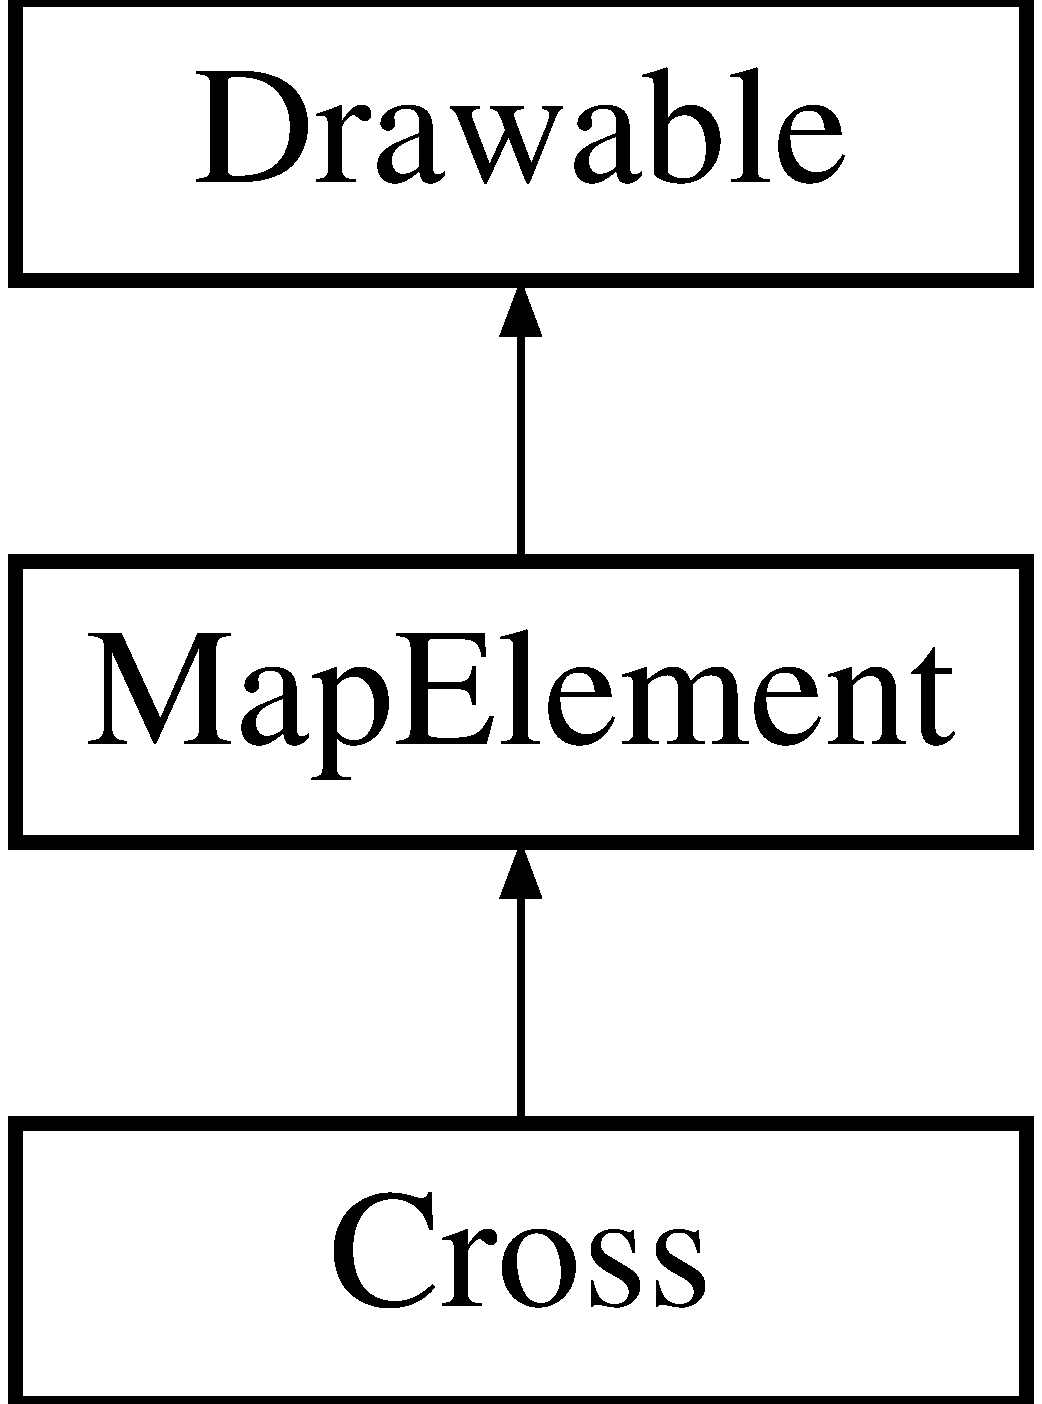
\includegraphics[height=3.000000cm]{class_cross}
\end{center}
\end{figure}
\subsection*{Metody publiczne}
\begin{DoxyCompactItemize}
\item 
\hyperlink{class_cross_ad0886f2b47a4375b7b6feedfc13c0692}{Cross} (int id\-\_\-, double x\-\_\-, double y\-\_\-, \hyperlink{class_priority_rules}{Priority\-Rules} $\ast$rules\-\_\-, map$<$ \hyperlink{_direction_8h_a224b9163917ac32fc95a60d8c1eec3aa}{Direction}, int $>$ neighbors\-\_\-)
\begin{DoxyCompactList}\small\item\em Konstruktor. \end{DoxyCompactList}\item 
\hyperlink{class_cross_afa046c5821fd92064ecfdcb2c28fae00}{Cross} (int id\-\_\-, \hyperlink{struct_position}{Position} position\-\_\-, \hyperlink{class_priority_rules}{Priority\-Rules} $\ast$rules\-\_\-, map$<$ \hyperlink{_direction_8h_a224b9163917ac32fc95a60d8c1eec3aa}{Direction}, int $>$ neighbors\-\_\-)
\begin{DoxyCompactList}\small\item\em Konstruktor. \end{DoxyCompactList}\item 
virtual \hyperlink{class_cross_a1d87d50bd56692c7ed29640b0f7d1d81}{$\sim$\-Cross} ()
\item 
virtual void \hyperlink{class_cross_a3b127c19a196ad86bbd27b513eecdf44}{draw} (\hyperlink{class_scene}{Scene} $\ast$scene)
\begin{DoxyCompactList}\small\item\em Metoda odpowiadająca za wyświetlenie skrzyżowania na scenie. \end{DoxyCompactList}\item 
void \hyperlink{class_cross_a01b9a1199aa8a1cc8f7c2a4268eb2656}{register\-Vehicle} (\hyperlink{_direction_8h_a224b9163917ac32fc95a60d8c1eec3aa}{Direction} direction\-\_\-, \hyperlink{class_vehicle}{Vehicle} $\ast$v\-\_\-)
\begin{DoxyCompactList}\small\item\em Rejestracja pojazdu w skrzyżowaniu. \end{DoxyCompactList}\item 
void \hyperlink{class_cross_a02405bee42d1e6faf6450d8198e1cb45}{unregister\-Vehicle} (\hyperlink{_direction_8h_a224b9163917ac32fc95a60d8c1eec3aa}{Direction} direction\-\_\-)
\begin{DoxyCompactList}\small\item\em Wyrejestrowanie pojazdu. \end{DoxyCompactList}\item 
bool \hyperlink{class_cross_a9c8223fd7c88d4ebfebf44eec3abfc87}{can\-Go} (\hyperlink{_direction_8h_a224b9163917ac32fc95a60d8c1eec3aa}{Direction} from\-\_\-, \hyperlink{_direction_8h_a224b9163917ac32fc95a60d8c1eec3aa}{Direction} to\-\_\-)
\begin{DoxyCompactList}\small\item\em Metoda zwraca przyzwolenie na wjazd na skrzyżowanie. \end{DoxyCompactList}\item 
\hyperlink{_direction_8h_a224b9163917ac32fc95a60d8c1eec3aa}{Direction} \hyperlink{class_cross_ac1bb07b4ecdaa59c3bc4ef1583424281}{get\-Neighbor\-Direction} (int id\-\_\-)
\begin{DoxyCompactList}\small\item\em Metoda zwraca kierunek w którym znajduje się sąsiad o danym I\-D. \end{DoxyCompactList}\item 
\hyperlink{_direction_8h_a224b9163917ac32fc95a60d8c1eec3aa}{Direction} \hyperlink{class_cross_a034afdc8547efdf62c44e05c276ed601}{get\-Random\-Direction} (int from\-\_\-)
\begin{DoxyCompactList}\small\item\em Metoda podaje losowy z dostepnych kierunków. \end{DoxyCompactList}\item 
\hyperlink{struct_position}{Position} \hyperlink{class_cross_a0e1bc9d7a602cfa4b1ffe22d9748c11c}{calculate\-Pedestrian\-Position} (\hyperlink{_direction_8h_a224b9163917ac32fc95a60d8c1eec3aa}{Direction} direction\-\_\-, int side\-\_\-)
\begin{DoxyCompactList}\small\item\em Metoda obliczająca pozycję startową dla przechodnia oraz informująca go gdzie jest chodnik. \end{DoxyCompactList}\item 
\hyperlink{_direction_8h_a224b9163917ac32fc95a60d8c1eec3aa}{Direction} \hyperlink{class_cross_a34bf1008f626560d8200a9b2b677abb3}{get\-Pedestrian\-Random\-Direction} ()
\begin{DoxyCompactList}\small\item\em Zwraca losowy z dostepnych kierunków dla ruchu pieszych. \end{DoxyCompactList}\end{DoxyCompactItemize}
\subsection*{Statyczne metody publiczne}
\begin{DoxyCompactItemize}
\item 
static bool \hyperlink{class_cross_a50997bb8f3f5fb2b850ec897b1f3912c}{is\-Cross} (const \hyperlink{_types_8h_a4260a5280323637f8a1fa28e89b6ef14}{P\-Map\-Element} el)
\begin{DoxyCompactList}\small\item\em funkcja sprawdzająca czy obiekt wskazywany przez P\-Map\-Element jest skrzyżowaniem \end{DoxyCompactList}\end{DoxyCompactItemize}
\subsection*{Atrybuty publiczne}
\begin{DoxyCompactItemize}
\item 
Q\-Graphics\-Item\-Group $\ast$ \hyperlink{class_cross_a62b3a18fc6fa317d516846efe454b8ae}{cross\-Group}
\end{DoxyCompactItemize}
\subsection*{Metody prywatne}
\begin{DoxyCompactItemize}
\item 
vector$<$ Q\-Graphics\-Ellipse\-Item $\ast$ $>$ \hyperlink{class_cross_acc4e85c6307c933995275b7c84916ca9}{draw\-Dot} (\hyperlink{class_cross_rules}{Cross\-Rules} $\ast$)
\end{DoxyCompactItemize}
\subsection*{Atrybuty prywatne}
\begin{DoxyCompactItemize}
\item 
\hyperlink{class_priority_rules}{Priority\-Rules} $\ast$ \hyperlink{class_cross_a46a8edfbb4172a050ceeba58db6c30bb}{priority\-Rules}
\item 
map$<$ \hyperlink{_direction_8h_a224b9163917ac32fc95a60d8c1eec3aa}{Direction}, int $>$ \hyperlink{class_cross_af931388763664ba4224f054b6a42fea2}{neighbors}
\item 
map$<$ \hyperlink{_direction_8h_a224b9163917ac32fc95a60d8c1eec3aa}{Direction}, vector\\*
$<$ \hyperlink{class_vehicle}{Vehicle} $\ast$ $>$ $>$ \hyperlink{class_cross_aa6994973a6c8e4d0478410dbeb47d3b4}{waiting\-Vehicles}
\end{DoxyCompactItemize}
\subsection*{Dodatkowe Dziedziczone Składowe}


\subsection{Opis szczegółowy}
Klasa reprezentujaca skrzyzowanie. 

\subsection{Dokumentacja konstruktora i destruktora}
\hypertarget{class_cross_ad0886f2b47a4375b7b6feedfc13c0692}{\index{Cross@{Cross}!Cross@{Cross}}
\index{Cross@{Cross}!Cross@{Cross}}
\subsubsection[{Cross}]{\setlength{\rightskip}{0pt plus 5cm}Cross\-::\-Cross (
\begin{DoxyParamCaption}
\item[{int}]{id\-\_\-, }
\item[{double}]{x\-\_\-, }
\item[{double}]{y\-\_\-, }
\item[{{\bf Priority\-Rules} $\ast$}]{rules\-\_\-, }
\item[{map$<$ {\bf Direction}, int $>$}]{neighbors\-\_\-}
\end{DoxyParamCaption}
)\hspace{0.3cm}{\ttfamily [inline]}}}\label{class_cross_ad0886f2b47a4375b7b6feedfc13c0692}


Konstruktor. 

\hypertarget{class_cross_afa046c5821fd92064ecfdcb2c28fae00}{\index{Cross@{Cross}!Cross@{Cross}}
\index{Cross@{Cross}!Cross@{Cross}}
\subsubsection[{Cross}]{\setlength{\rightskip}{0pt plus 5cm}Cross\-::\-Cross (
\begin{DoxyParamCaption}
\item[{int}]{id\-\_\-, }
\item[{{\bf Position}}]{position\-\_\-, }
\item[{{\bf Priority\-Rules} $\ast$}]{rules\-\_\-, }
\item[{map$<$ {\bf Direction}, int $>$}]{neighbors\-\_\-}
\end{DoxyParamCaption}
)\hspace{0.3cm}{\ttfamily [inline]}}}\label{class_cross_afa046c5821fd92064ecfdcb2c28fae00}


Konstruktor. 

\hypertarget{class_cross_a1d87d50bd56692c7ed29640b0f7d1d81}{\index{Cross@{Cross}!$\sim$\-Cross@{$\sim$\-Cross}}
\index{$\sim$\-Cross@{$\sim$\-Cross}!Cross@{Cross}}
\subsubsection[{$\sim$\-Cross}]{\setlength{\rightskip}{0pt plus 5cm}virtual Cross\-::$\sim$\-Cross (
\begin{DoxyParamCaption}
{}
\end{DoxyParamCaption}
)\hspace{0.3cm}{\ttfamily [inline]}, {\ttfamily [virtual]}}}\label{class_cross_a1d87d50bd56692c7ed29640b0f7d1d81}


\subsection{Dokumentacja funkcji składowych}
\hypertarget{class_cross_a0e1bc9d7a602cfa4b1ffe22d9748c11c}{\index{Cross@{Cross}!calculate\-Pedestrian\-Position@{calculate\-Pedestrian\-Position}}
\index{calculate\-Pedestrian\-Position@{calculate\-Pedestrian\-Position}!Cross@{Cross}}
\subsubsection[{calculate\-Pedestrian\-Position}]{\setlength{\rightskip}{0pt plus 5cm}{\bf Position} Cross\-::calculate\-Pedestrian\-Position (
\begin{DoxyParamCaption}
\item[{{\bf Direction}}]{direction\-\_\-, }
\item[{int}]{side\-\_\-}
\end{DoxyParamCaption}
)}}\label{class_cross_a0e1bc9d7a602cfa4b1ffe22d9748c11c}


Metoda obliczająca pozycję startową dla przechodnia oraz informująca go gdzie jest chodnik. 

\hypertarget{class_cross_a9c8223fd7c88d4ebfebf44eec3abfc87}{\index{Cross@{Cross}!can\-Go@{can\-Go}}
\index{can\-Go@{can\-Go}!Cross@{Cross}}
\subsubsection[{can\-Go}]{\setlength{\rightskip}{0pt plus 5cm}bool Cross\-::can\-Go (
\begin{DoxyParamCaption}
\item[{{\bf Direction}}]{from\-\_\-, }
\item[{{\bf Direction}}]{to\-\_\-}
\end{DoxyParamCaption}
)}}\label{class_cross_a9c8223fd7c88d4ebfebf44eec3abfc87}


Metoda zwraca przyzwolenie na wjazd na skrzyżowanie. 

\hypertarget{class_cross_a3b127c19a196ad86bbd27b513eecdf44}{\index{Cross@{Cross}!draw@{draw}}
\index{draw@{draw}!Cross@{Cross}}
\subsubsection[{draw}]{\setlength{\rightskip}{0pt plus 5cm}void Cross\-::draw (
\begin{DoxyParamCaption}
\item[{{\bf Scene} $\ast$}]{scene}
\end{DoxyParamCaption}
)\hspace{0.3cm}{\ttfamily [virtual]}}}\label{class_cross_a3b127c19a196ad86bbd27b513eecdf44}


Metoda odpowiadająca za wyświetlenie skrzyżowania na scenie. 



Implementuje \hyperlink{class_map_element_aa76ca7443c4f6a6683f68f44909b90d3}{Map\-Element}.

\hypertarget{class_cross_acc4e85c6307c933995275b7c84916ca9}{\index{Cross@{Cross}!draw\-Dot@{draw\-Dot}}
\index{draw\-Dot@{draw\-Dot}!Cross@{Cross}}
\subsubsection[{draw\-Dot}]{\setlength{\rightskip}{0pt plus 5cm}vector$<$ Q\-Graphics\-Ellipse\-Item $\ast$ $>$ Cross\-::draw\-Dot (
\begin{DoxyParamCaption}
\item[{{\bf Cross\-Rules} $\ast$}]{cr}
\end{DoxyParamCaption}
)\hspace{0.3cm}{\ttfamily [private]}}}\label{class_cross_acc4e85c6307c933995275b7c84916ca9}
\hypertarget{class_cross_ac1bb07b4ecdaa59c3bc4ef1583424281}{\index{Cross@{Cross}!get\-Neighbor\-Direction@{get\-Neighbor\-Direction}}
\index{get\-Neighbor\-Direction@{get\-Neighbor\-Direction}!Cross@{Cross}}
\subsubsection[{get\-Neighbor\-Direction}]{\setlength{\rightskip}{0pt plus 5cm}{\bf Direction} Cross\-::get\-Neighbor\-Direction (
\begin{DoxyParamCaption}
\item[{int}]{id\-\_\-}
\end{DoxyParamCaption}
)}}\label{class_cross_ac1bb07b4ecdaa59c3bc4ef1583424281}


Metoda zwraca kierunek w którym znajduje się sąsiad o danym I\-D. 

\hypertarget{class_cross_a34bf1008f626560d8200a9b2b677abb3}{\index{Cross@{Cross}!get\-Pedestrian\-Random\-Direction@{get\-Pedestrian\-Random\-Direction}}
\index{get\-Pedestrian\-Random\-Direction@{get\-Pedestrian\-Random\-Direction}!Cross@{Cross}}
\subsubsection[{get\-Pedestrian\-Random\-Direction}]{\setlength{\rightskip}{0pt plus 5cm}{\bf Direction} Cross\-::get\-Pedestrian\-Random\-Direction (
\begin{DoxyParamCaption}
{}
\end{DoxyParamCaption}
)}}\label{class_cross_a34bf1008f626560d8200a9b2b677abb3}


Zwraca losowy z dostepnych kierunków dla ruchu pieszych. 

\hypertarget{class_cross_a034afdc8547efdf62c44e05c276ed601}{\index{Cross@{Cross}!get\-Random\-Direction@{get\-Random\-Direction}}
\index{get\-Random\-Direction@{get\-Random\-Direction}!Cross@{Cross}}
\subsubsection[{get\-Random\-Direction}]{\setlength{\rightskip}{0pt plus 5cm}{\bf Direction} Cross\-::get\-Random\-Direction (
\begin{DoxyParamCaption}
\item[{int}]{from\-\_\-}
\end{DoxyParamCaption}
)}}\label{class_cross_a034afdc8547efdf62c44e05c276ed601}


Metoda podaje losowy z dostepnych kierunków. 

\hypertarget{class_cross_a50997bb8f3f5fb2b850ec897b1f3912c}{\index{Cross@{Cross}!is\-Cross@{is\-Cross}}
\index{is\-Cross@{is\-Cross}!Cross@{Cross}}
\subsubsection[{is\-Cross}]{\setlength{\rightskip}{0pt plus 5cm}bool Cross\-::is\-Cross (
\begin{DoxyParamCaption}
\item[{const {\bf P\-Map\-Element}}]{el}
\end{DoxyParamCaption}
)\hspace{0.3cm}{\ttfamily [static]}}}\label{class_cross_a50997bb8f3f5fb2b850ec897b1f3912c}


funkcja sprawdzająca czy obiekt wskazywany przez P\-Map\-Element jest skrzyżowaniem 

\hypertarget{class_cross_a01b9a1199aa8a1cc8f7c2a4268eb2656}{\index{Cross@{Cross}!register\-Vehicle@{register\-Vehicle}}
\index{register\-Vehicle@{register\-Vehicle}!Cross@{Cross}}
\subsubsection[{register\-Vehicle}]{\setlength{\rightskip}{0pt plus 5cm}void Cross\-::register\-Vehicle (
\begin{DoxyParamCaption}
\item[{{\bf Direction}}]{direction\-\_\-, }
\item[{{\bf Vehicle} $\ast$}]{v\-\_\-}
\end{DoxyParamCaption}
)}}\label{class_cross_a01b9a1199aa8a1cc8f7c2a4268eb2656}


Rejestracja pojazdu w skrzyżowaniu. 

\hypertarget{class_cross_a02405bee42d1e6faf6450d8198e1cb45}{\index{Cross@{Cross}!unregister\-Vehicle@{unregister\-Vehicle}}
\index{unregister\-Vehicle@{unregister\-Vehicle}!Cross@{Cross}}
\subsubsection[{unregister\-Vehicle}]{\setlength{\rightskip}{0pt plus 5cm}void Cross\-::unregister\-Vehicle (
\begin{DoxyParamCaption}
\item[{{\bf Direction}}]{direction\-\_\-}
\end{DoxyParamCaption}
)}}\label{class_cross_a02405bee42d1e6faf6450d8198e1cb45}


Wyrejestrowanie pojazdu. 



\subsection{Dokumentacja atrybutów składowych}
\hypertarget{class_cross_a62b3a18fc6fa317d516846efe454b8ae}{\index{Cross@{Cross}!cross\-Group@{cross\-Group}}
\index{cross\-Group@{cross\-Group}!Cross@{Cross}}
\subsubsection[{cross\-Group}]{\setlength{\rightskip}{0pt plus 5cm}Q\-Graphics\-Item\-Group$\ast$ Cross\-::cross\-Group}}\label{class_cross_a62b3a18fc6fa317d516846efe454b8ae}
\hypertarget{class_cross_af931388763664ba4224f054b6a42fea2}{\index{Cross@{Cross}!neighbors@{neighbors}}
\index{neighbors@{neighbors}!Cross@{Cross}}
\subsubsection[{neighbors}]{\setlength{\rightskip}{0pt plus 5cm}map$<${\bf Direction}, int$>$ Cross\-::neighbors\hspace{0.3cm}{\ttfamily [private]}}}\label{class_cross_af931388763664ba4224f054b6a42fea2}
\hypertarget{class_cross_a46a8edfbb4172a050ceeba58db6c30bb}{\index{Cross@{Cross}!priority\-Rules@{priority\-Rules}}
\index{priority\-Rules@{priority\-Rules}!Cross@{Cross}}
\subsubsection[{priority\-Rules}]{\setlength{\rightskip}{0pt plus 5cm}{\bf Priority\-Rules}$\ast$ Cross\-::priority\-Rules\hspace{0.3cm}{\ttfamily [private]}}}\label{class_cross_a46a8edfbb4172a050ceeba58db6c30bb}
\hypertarget{class_cross_aa6994973a6c8e4d0478410dbeb47d3b4}{\index{Cross@{Cross}!waiting\-Vehicles@{waiting\-Vehicles}}
\index{waiting\-Vehicles@{waiting\-Vehicles}!Cross@{Cross}}
\subsubsection[{waiting\-Vehicles}]{\setlength{\rightskip}{0pt plus 5cm}map$<${\bf Direction}, vector$<${\bf Vehicle}$\ast$$>$ $>$ Cross\-::waiting\-Vehicles\hspace{0.3cm}{\ttfamily [private]}}}\label{class_cross_aa6994973a6c8e4d0478410dbeb47d3b4}


Dokumentacja dla tej klasy została wygenerowana z plików\-:\begin{DoxyCompactItemize}
\item 
src/\hyperlink{_cross_8h}{Cross.\-h}\item 
src/\hyperlink{_cross_8cpp}{Cross.\-cpp}\end{DoxyCompactItemize}

\hypertarget{class_cross_rules}{\section{Dokumentacja klasy Cross\-Rules}
\label{class_cross_rules}\index{Cross\-Rules@{Cross\-Rules}}
}


Klasa podająca informacje o pierwszeństwie przejazdu.  




{\ttfamily \#include $<$Cross\-Rules.\-h$>$}

Diagram dziedziczenia dla Cross\-Rules\begin{figure}[H]
\begin{center}
\leavevmode
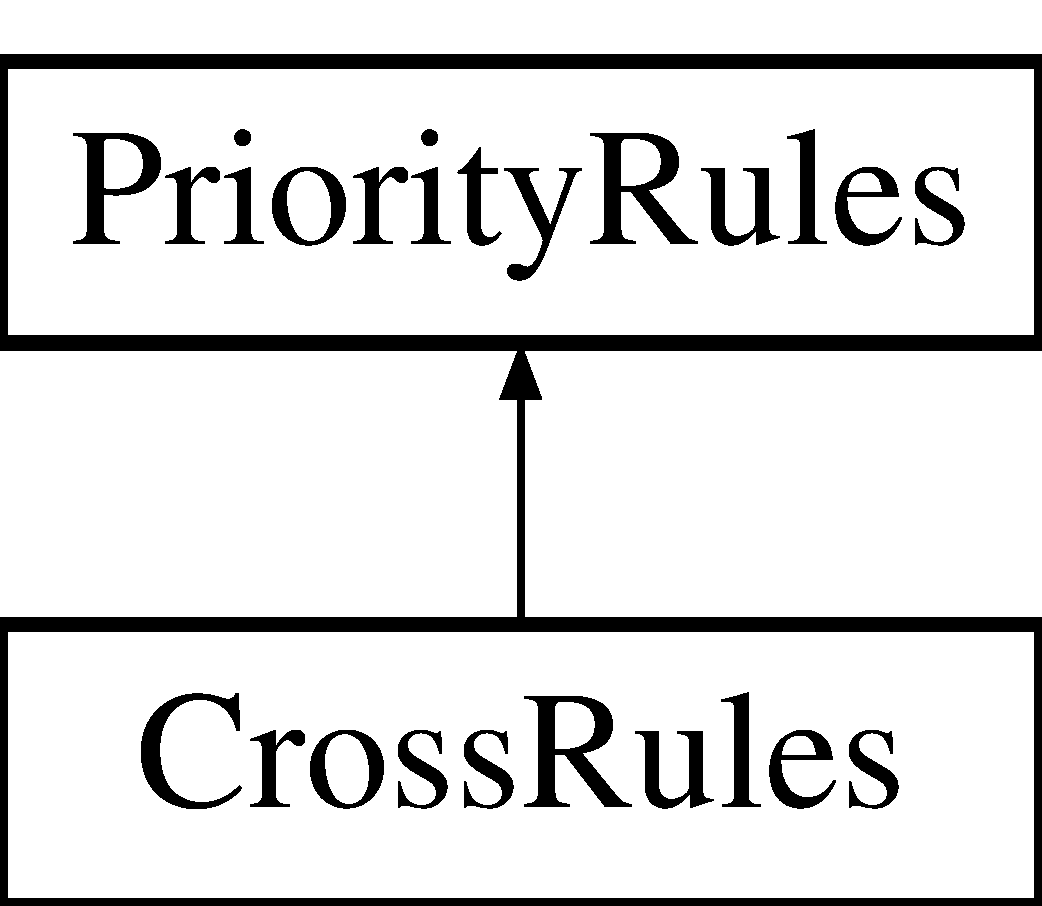
\includegraphics[height=2.000000cm]{class_cross_rules}
\end{center}
\end{figure}
\subsection*{Metody publiczne}
\begin{DoxyCompactItemize}
\item 
\hyperlink{class_cross_rules_abb95f00b153b70701e01ca5890139c01}{Cross\-Rules} (vector$<$ char $>$ subordinate\-\_\-, map$<$ \hyperlink{_direction_8h_a224b9163917ac32fc95a60d8c1eec3aa}{Direction}, int $>$ directions\-\_\-)
\begin{DoxyCompactList}\small\item\em Konstruktor. \end{DoxyCompactList}\item 
virtual set$<$ \hyperlink{_direction_8h_a224b9163917ac32fc95a60d8c1eec3aa}{Direction} $>$ \hyperlink{class_cross_rules_afc553f8d0a643382b188ebd95faca30f}{get\-Rules} (\hyperlink{_direction_8h_a224b9163917ac32fc95a60d8c1eec3aa}{Direction} from\-\_\-, \hyperlink{_direction_8h_a224b9163917ac32fc95a60d8c1eec3aa}{Direction} to\-\_\-)
\begin{DoxyCompactList}\small\item\em Metoda zwraca zasady pierwszeństwa. \end{DoxyCompactList}\item 
bool \hyperlink{class_cross_rules_aa4799b5462b003f34316a0abf7968d68}{is\-Subordinate} (\hyperlink{_direction_8h_a224b9163917ac32fc95a60d8c1eec3aa}{Direction} direction\-\_\-)
\end{DoxyCompactItemize}
\subsection*{Atrybuty prywatne}
\begin{DoxyCompactItemize}
\item 
vector$<$ int $>$ \hyperlink{class_cross_rules_a60e45af96fe44c6fa7eef1197ba621dd}{rules}
\end{DoxyCompactItemize}


\subsection{Opis szczegółowy}
Klasa podająca informacje o pierwszeństwie przejazdu. 

\subsection{Dokumentacja konstruktora i destruktora}
\hypertarget{class_cross_rules_abb95f00b153b70701e01ca5890139c01}{\index{Cross\-Rules@{Cross\-Rules}!Cross\-Rules@{Cross\-Rules}}
\index{Cross\-Rules@{Cross\-Rules}!CrossRules@{Cross\-Rules}}
\subsubsection[{Cross\-Rules}]{\setlength{\rightskip}{0pt plus 5cm}Cross\-Rules\-::\-Cross\-Rules (
\begin{DoxyParamCaption}
\item[{vector$<$ char $>$}]{subordinate\-\_\-, }
\item[{map$<$ {\bf Direction}, int $>$}]{directions\-\_\-}
\end{DoxyParamCaption}
)}}\label{class_cross_rules_abb95f00b153b70701e01ca5890139c01}


Konstruktor. 



\subsection{Dokumentacja funkcji składowych}
\hypertarget{class_cross_rules_afc553f8d0a643382b188ebd95faca30f}{\index{Cross\-Rules@{Cross\-Rules}!get\-Rules@{get\-Rules}}
\index{get\-Rules@{get\-Rules}!CrossRules@{Cross\-Rules}}
\subsubsection[{get\-Rules}]{\setlength{\rightskip}{0pt plus 5cm}set$<$ {\bf Direction} $>$ Cross\-Rules\-::get\-Rules (
\begin{DoxyParamCaption}
\item[{{\bf Direction}}]{from\-\_\-, }
\item[{{\bf Direction}}]{to\-\_\-}
\end{DoxyParamCaption}
)\hspace{0.3cm}{\ttfamily [virtual]}}}\label{class_cross_rules_afc553f8d0a643382b188ebd95faca30f}


Metoda zwraca zasady pierwszeństwa. 



Implementuje \hyperlink{class_priority_rules_a1a64b70868b8c50ebe6bbc01062da361}{Priority\-Rules}.

\hypertarget{class_cross_rules_aa4799b5462b003f34316a0abf7968d68}{\index{Cross\-Rules@{Cross\-Rules}!is\-Subordinate@{is\-Subordinate}}
\index{is\-Subordinate@{is\-Subordinate}!CrossRules@{Cross\-Rules}}
\subsubsection[{is\-Subordinate}]{\setlength{\rightskip}{0pt plus 5cm}bool Cross\-Rules\-::is\-Subordinate (
\begin{DoxyParamCaption}
\item[{{\bf Direction}}]{direction\-\_\-}
\end{DoxyParamCaption}
)}}\label{class_cross_rules_aa4799b5462b003f34316a0abf7968d68}


\subsection{Dokumentacja atrybutów składowych}
\hypertarget{class_cross_rules_a60e45af96fe44c6fa7eef1197ba621dd}{\index{Cross\-Rules@{Cross\-Rules}!rules@{rules}}
\index{rules@{rules}!CrossRules@{Cross\-Rules}}
\subsubsection[{rules}]{\setlength{\rightskip}{0pt plus 5cm}vector$<$int$>$ Cross\-Rules\-::rules\hspace{0.3cm}{\ttfamily [private]}}}\label{class_cross_rules_a60e45af96fe44c6fa7eef1197ba621dd}


Dokumentacja dla tej klasy została wygenerowana z plików\-:\begin{DoxyCompactItemize}
\item 
src/\hyperlink{_cross_rules_8h}{Cross\-Rules.\-h}\item 
src/\hyperlink{_cross_rules_8cpp}{Cross\-Rules.\-cpp}\end{DoxyCompactItemize}

\hypertarget{class_drawable}{\section{Dokumentacja klasy Drawable}
\label{class_drawable}\index{Drawable@{Drawable}}
}


Klasa bazowa dla obiektów, które będą wyświetlane na scenie.  




{\ttfamily \#include $<$Drawable.\-h$>$}

Diagram dziedziczenia dla Drawable\begin{figure}[H]
\begin{center}
\leavevmode
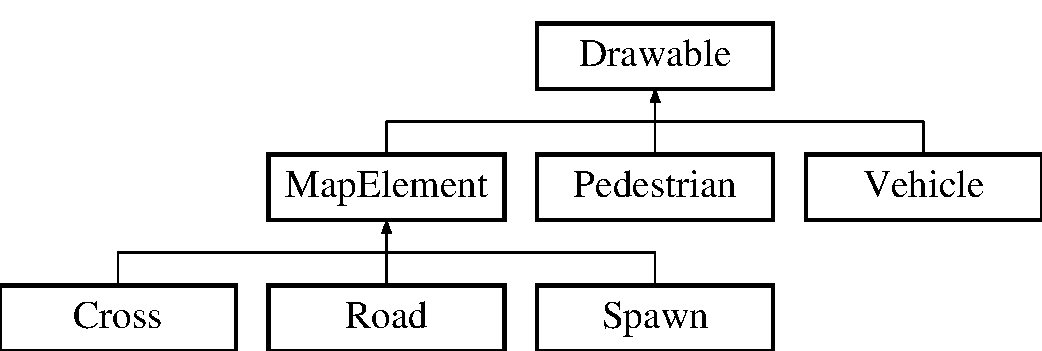
\includegraphics[height=3.000000cm]{class_drawable}
\end{center}
\end{figure}
\subsection*{Metody publiczne}
\begin{DoxyCompactItemize}
\item 
\hyperlink{class_drawable_acdf5ee89ba1c083f4162cfd892c1989c}{Drawable} (\hyperlink{struct_position}{Position} position\-\_\-)
\begin{DoxyCompactList}\small\item\em Konstruktor. \end{DoxyCompactList}\item 
\hyperlink{class_drawable_a7799a0919cf41e051ef48f2467a8686f}{Drawable} (double x\-\_\-, double y\-\_\-, double z\-\_\-=0)
\begin{DoxyCompactList}\small\item\em Konstruktor. \end{DoxyCompactList}\item 
virtual void \hyperlink{class_drawable_a1e24b799e5b5f5494b25a42e2624692c}{draw} (\hyperlink{class_scene}{Scene} $\ast$scene)=0
\item 
\hyperlink{struct_position}{Position} \hyperlink{class_drawable_ae9383e020b150097521c248763c071fa}{get\-Position} () const 
\begin{DoxyCompactList}\small\item\em Zwraca pozycję obiektu. \end{DoxyCompactList}\item 
void \hyperlink{class_drawable_ab4a98a7b3e4fd76a2d14b9f1d51c3a41}{set\-Position} (const double x\-\_\-, const double y\-\_\-)
\begin{DoxyCompactList}\small\item\em Ustawia pozycję obiektu. \end{DoxyCompactList}\item 
void \hyperlink{class_drawable_afa4dae6843185ee5a2cdaf79325099a5}{set\-Position} (const \hyperlink{struct_position}{Position} position\-\_\-)
\begin{DoxyCompactList}\small\item\em Ustawia pozycję obiektu. \end{DoxyCompactList}\end{DoxyCompactItemize}
\subsection*{Atrybuty chronione}
\begin{DoxyCompactItemize}
\item 
\hyperlink{struct_position}{Position} \hyperlink{class_drawable_aaeba34b10714af371e05d44d825af8a5}{position}
\end{DoxyCompactItemize}


\subsection{Opis szczegółowy}
Klasa bazowa dla obiektów, które będą wyświetlane na scenie. 

\subsection{Dokumentacja konstruktora i destruktora}
\hypertarget{class_drawable_acdf5ee89ba1c083f4162cfd892c1989c}{\index{Drawable@{Drawable}!Drawable@{Drawable}}
\index{Drawable@{Drawable}!Drawable@{Drawable}}
\subsubsection[{Drawable}]{\setlength{\rightskip}{0pt plus 5cm}Drawable\-::\-Drawable (
\begin{DoxyParamCaption}
\item[{{\bf Position}}]{position\-\_\-}
\end{DoxyParamCaption}
)\hspace{0.3cm}{\ttfamily [inline]}}}\label{class_drawable_acdf5ee89ba1c083f4162cfd892c1989c}


Konstruktor. 

\hypertarget{class_drawable_a7799a0919cf41e051ef48f2467a8686f}{\index{Drawable@{Drawable}!Drawable@{Drawable}}
\index{Drawable@{Drawable}!Drawable@{Drawable}}
\subsubsection[{Drawable}]{\setlength{\rightskip}{0pt plus 5cm}Drawable\-::\-Drawable (
\begin{DoxyParamCaption}
\item[{double}]{x\-\_\-, }
\item[{double}]{y\-\_\-, }
\item[{double}]{z\-\_\- = {\ttfamily 0}}
\end{DoxyParamCaption}
)\hspace{0.3cm}{\ttfamily [inline]}}}\label{class_drawable_a7799a0919cf41e051ef48f2467a8686f}


Konstruktor. 



\subsection{Dokumentacja funkcji składowych}
\hypertarget{class_drawable_a1e24b799e5b5f5494b25a42e2624692c}{\index{Drawable@{Drawable}!draw@{draw}}
\index{draw@{draw}!Drawable@{Drawable}}
\subsubsection[{draw}]{\setlength{\rightskip}{0pt plus 5cm}virtual void Drawable\-::draw (
\begin{DoxyParamCaption}
\item[{{\bf Scene} $\ast$}]{scene}
\end{DoxyParamCaption}
)\hspace{0.3cm}{\ttfamily [pure virtual]}}}\label{class_drawable_a1e24b799e5b5f5494b25a42e2624692c}


Implementowany w \hyperlink{class_vehicle_a91c55b0a0ffc22c4f759452332b9ecd0}{Vehicle}, \hyperlink{class_cross_a3b127c19a196ad86bbd27b513eecdf44}{Cross}, \hyperlink{class_pedestrian_a51d926e2af8c607afef85f5e4d169a7a}{Pedestrian}, \hyperlink{class_spawn_a725ac9cb33aff1b26b19ed3affecf692}{Spawn}, \hyperlink{class_map_element_aa76ca7443c4f6a6683f68f44909b90d3}{Map\-Element} i \hyperlink{class_road_a276332c2d6a617ca0fc665470fc49901}{Road}.

\hypertarget{class_drawable_ae9383e020b150097521c248763c071fa}{\index{Drawable@{Drawable}!get\-Position@{get\-Position}}
\index{get\-Position@{get\-Position}!Drawable@{Drawable}}
\subsubsection[{get\-Position}]{\setlength{\rightskip}{0pt plus 5cm}{\bf Position} Drawable\-::get\-Position (
\begin{DoxyParamCaption}
{}
\end{DoxyParamCaption}
) const\hspace{0.3cm}{\ttfamily [inline]}}}\label{class_drawable_ae9383e020b150097521c248763c071fa}


Zwraca pozycję obiektu. 

\hypertarget{class_drawable_ab4a98a7b3e4fd76a2d14b9f1d51c3a41}{\index{Drawable@{Drawable}!set\-Position@{set\-Position}}
\index{set\-Position@{set\-Position}!Drawable@{Drawable}}
\subsubsection[{set\-Position}]{\setlength{\rightskip}{0pt plus 5cm}void Drawable\-::set\-Position (
\begin{DoxyParamCaption}
\item[{const double}]{x\-\_\-, }
\item[{const double}]{y\-\_\-}
\end{DoxyParamCaption}
)\hspace{0.3cm}{\ttfamily [inline]}}}\label{class_drawable_ab4a98a7b3e4fd76a2d14b9f1d51c3a41}


Ustawia pozycję obiektu. 

\hypertarget{class_drawable_afa4dae6843185ee5a2cdaf79325099a5}{\index{Drawable@{Drawable}!set\-Position@{set\-Position}}
\index{set\-Position@{set\-Position}!Drawable@{Drawable}}
\subsubsection[{set\-Position}]{\setlength{\rightskip}{0pt plus 5cm}void Drawable\-::set\-Position (
\begin{DoxyParamCaption}
\item[{const {\bf Position}}]{position\-\_\-}
\end{DoxyParamCaption}
)\hspace{0.3cm}{\ttfamily [inline]}}}\label{class_drawable_afa4dae6843185ee5a2cdaf79325099a5}


Ustawia pozycję obiektu. 



\subsection{Dokumentacja atrybutów składowych}
\hypertarget{class_drawable_aaeba34b10714af371e05d44d825af8a5}{\index{Drawable@{Drawable}!position@{position}}
\index{position@{position}!Drawable@{Drawable}}
\subsubsection[{position}]{\setlength{\rightskip}{0pt plus 5cm}{\bf Position} Drawable\-::position\hspace{0.3cm}{\ttfamily [protected]}}}\label{class_drawable_aaeba34b10714af371e05d44d825af8a5}


Dokumentacja dla tej klasy została wygenerowana z pliku\-:\begin{DoxyCompactItemize}
\item 
src/\hyperlink{_drawable_8h}{Drawable.\-h}\end{DoxyCompactItemize}

\hypertarget{class_main_window}{\section{Dokumentacja klasy Main\-Window}
\label{class_main_window}\index{Main\-Window@{Main\-Window}}
}


Klasa głównego okna aplikacji.  




{\ttfamily \#include $<$Main\-Window.\-h$>$}

\subsection*{Sloty publiczne}
\begin{DoxyCompactItemize}
\item 
void \hyperlink{class_main_window_a524779fedd6fbedd87913f9e38d059aa}{start\-Button\-Clicked} ()
\begin{DoxyCompactList}\small\item\em Slot wykonujący dzialanie po naciśnięciu przycisku Start. \end{DoxyCompactList}\item 
void \hyperlink{class_main_window_ad59e90d0dd01444e222c94421dbfb1aa}{add\-Camera\-Button\-Clicked} ()
\begin{DoxyCompactList}\small\item\em Slot wykonujący dzialanie po naciśnięciu przycisku Add \hyperlink{class_camera}{Camera}. \end{DoxyCompactList}\item 
void \hyperlink{class_main_window_a391c23cbe0aea03008357c96c89d79e0}{save\-Camera\-Log\-Button\-Clicked} ()
\begin{DoxyCompactList}\small\item\em Slot wykonujący dzialanie po naciśnięciu przycisku Save Log. \end{DoxyCompactList}\item 
void \hyperlink{class_main_window_acfe9790838bda5b46ccc90c2760822ba}{camera\-Event} (Q\-String)
\begin{DoxyCompactList}\small\item\em Slot przyjmujący wiadomości od kamer. Wyświetla je w Q\-Text\-Edit. \end{DoxyCompactList}\item 
void \hyperlink{class_main_window_a52d6970c3dcddf7c1ed65ff435743bc3}{show\-Exception\-Dialog} (Q\-String)
\begin{DoxyCompactList}\small\item\em Slot wyświeltający okienko z treścią wyjątku. \end{DoxyCompactList}\end{DoxyCompactItemize}
\subsection*{Metody publiczne}
\begin{DoxyCompactItemize}
\item 
\hyperlink{class_main_window_a8b244be8b7b7db1b08de2a2acb9409db}{Main\-Window} (Q\-Widget $\ast$parent=0)
\begin{DoxyCompactList}\small\item\em Konstruktor. \end{DoxyCompactList}\item 
\hyperlink{class_main_window_ae98d00a93bc118200eeef9f9bba1dba7}{$\sim$\-Main\-Window} ()
\end{DoxyCompactItemize}
\subsection*{Atrybuty publiczne}
\begin{DoxyCompactItemize}
\item 
\hyperlink{class_scene}{Scene} $\ast$ \hyperlink{class_main_window_a5fac52928ceff08c8137f4689aee3874}{scene}
\begin{DoxyCompactList}\small\item\em Wskaźnik na obiekt \hyperlink{class_scene}{Scene}. \end{DoxyCompactList}\item 
\hyperlink{class_simulator}{Simulator} $\ast$ \hyperlink{class_main_window_a0bb9399936b67eb8dba43b80443c0469}{simulator}
\begin{DoxyCompactList}\small\item\em Wskaźnik na obiekt \hyperlink{class_simulator}{Simulator}. \end{DoxyCompactList}\item 
\hyperlink{class_camera_controller}{Camera\-Controller} $\ast$ \hyperlink{class_main_window_a5db1869c49b5f061ee85f0843ba7d6f9}{camera\-Controller}
\begin{DoxyCompactList}\small\item\em Wskaźnik na obiekt \hyperlink{class_camera_controller}{Camera\-Controller}. \end{DoxyCompactList}\end{DoxyCompactItemize}
\subsection*{Metody chronione}
\begin{DoxyCompactItemize}
\item 
void \hyperlink{class_main_window_aa353e8faed952a95e2fc62d7a5018a89}{setup\-Ui} ()
\item 
void \hyperlink{class_main_window_a8851a931482834eeec527490eedaf20e}{resize\-Event} (Q\-Resize\-Event $\ast$)
\item 
void \hyperlink{class_main_window_a38edb88d43e844aca9d2e762c8706565}{close\-Event} (Q\-Close\-Event $\ast$)
\end{DoxyCompactItemize}
\subsection*{Atrybuty chronione}
\begin{DoxyCompactItemize}
\item 
Q\-Grid\-Layout $\ast$ \hyperlink{class_main_window_a16d41d6fadc8befa5afa12460580334a}{grid\-Layout}
\item 
Q\-Push\-Button $\ast$ \hyperlink{class_main_window_a209284547cc0a28bb29f55e5fd4e570a}{start\-Button}
\item 
Q\-Push\-Button $\ast$ \hyperlink{class_main_window_a57be70fafedbc093231447e86720672f}{add\-Camera\-Button}
\item 
Q\-Push\-Button $\ast$ \hyperlink{class_main_window_aec7ac81c3d7701401f21e91b5f843dec}{save\-Camera\-Log\-Button}
\item 
Q\-Text\-Edit $\ast$ \hyperlink{class_main_window_acb3521a7e05db17e12240ed82dcaa8d0}{camera\-Events\-Edit}
\item 
Q\-Graphics\-View $\ast$ \hyperlink{class_main_window_a2ae234c8fc9c4a897231f2ead4ad6d29}{graphics\-View}
\end{DoxyCompactItemize}


\subsection{Opis szczegółowy}
Klasa głównego okna aplikacji. 

\subsection{Dokumentacja konstruktora i destruktora}
\hypertarget{class_main_window_a8b244be8b7b7db1b08de2a2acb9409db}{\index{Main\-Window@{Main\-Window}!Main\-Window@{Main\-Window}}
\index{Main\-Window@{Main\-Window}!MainWindow@{Main\-Window}}
\subsubsection[{Main\-Window}]{\setlength{\rightskip}{0pt plus 5cm}Main\-Window\-::\-Main\-Window (
\begin{DoxyParamCaption}
\item[{Q\-Widget $\ast$}]{parent = {\ttfamily 0}}
\end{DoxyParamCaption}
)}}\label{class_main_window_a8b244be8b7b7db1b08de2a2acb9409db}


Konstruktor. 

\hypertarget{class_main_window_ae98d00a93bc118200eeef9f9bba1dba7}{\index{Main\-Window@{Main\-Window}!$\sim$\-Main\-Window@{$\sim$\-Main\-Window}}
\index{$\sim$\-Main\-Window@{$\sim$\-Main\-Window}!MainWindow@{Main\-Window}}
\subsubsection[{$\sim$\-Main\-Window}]{\setlength{\rightskip}{0pt plus 5cm}Main\-Window\-::$\sim$\-Main\-Window (
\begin{DoxyParamCaption}
{}
\end{DoxyParamCaption}
)}}\label{class_main_window_ae98d00a93bc118200eeef9f9bba1dba7}


\subsection{Dokumentacja funkcji składowych}
\hypertarget{class_main_window_ad59e90d0dd01444e222c94421dbfb1aa}{\index{Main\-Window@{Main\-Window}!add\-Camera\-Button\-Clicked@{add\-Camera\-Button\-Clicked}}
\index{add\-Camera\-Button\-Clicked@{add\-Camera\-Button\-Clicked}!MainWindow@{Main\-Window}}
\subsubsection[{add\-Camera\-Button\-Clicked}]{\setlength{\rightskip}{0pt plus 5cm}void Main\-Window\-::add\-Camera\-Button\-Clicked (
\begin{DoxyParamCaption}
{}
\end{DoxyParamCaption}
)\hspace{0.3cm}{\ttfamily [slot]}}}\label{class_main_window_ad59e90d0dd01444e222c94421dbfb1aa}


Slot wykonujący dzialanie po naciśnięciu przycisku Add \hyperlink{class_camera}{Camera}. 

\hypertarget{class_main_window_acfe9790838bda5b46ccc90c2760822ba}{\index{Main\-Window@{Main\-Window}!camera\-Event@{camera\-Event}}
\index{camera\-Event@{camera\-Event}!MainWindow@{Main\-Window}}
\subsubsection[{camera\-Event}]{\setlength{\rightskip}{0pt plus 5cm}void Main\-Window\-::camera\-Event (
\begin{DoxyParamCaption}
\item[{Q\-String}]{info}
\end{DoxyParamCaption}
)\hspace{0.3cm}{\ttfamily [slot]}}}\label{class_main_window_acfe9790838bda5b46ccc90c2760822ba}


Slot przyjmujący wiadomości od kamer. Wyświetla je w Q\-Text\-Edit. 

\hypertarget{class_main_window_a38edb88d43e844aca9d2e762c8706565}{\index{Main\-Window@{Main\-Window}!close\-Event@{close\-Event}}
\index{close\-Event@{close\-Event}!MainWindow@{Main\-Window}}
\subsubsection[{close\-Event}]{\setlength{\rightskip}{0pt plus 5cm}void Main\-Window\-::close\-Event (
\begin{DoxyParamCaption}
\item[{Q\-Close\-Event $\ast$}]{}
\end{DoxyParamCaption}
)\hspace{0.3cm}{\ttfamily [protected]}}}\label{class_main_window_a38edb88d43e844aca9d2e762c8706565}
\hypertarget{class_main_window_a8851a931482834eeec527490eedaf20e}{\index{Main\-Window@{Main\-Window}!resize\-Event@{resize\-Event}}
\index{resize\-Event@{resize\-Event}!MainWindow@{Main\-Window}}
\subsubsection[{resize\-Event}]{\setlength{\rightskip}{0pt plus 5cm}void Main\-Window\-::resize\-Event (
\begin{DoxyParamCaption}
\item[{Q\-Resize\-Event $\ast$}]{}
\end{DoxyParamCaption}
)\hspace{0.3cm}{\ttfamily [protected]}}}\label{class_main_window_a8851a931482834eeec527490eedaf20e}
\hypertarget{class_main_window_a391c23cbe0aea03008357c96c89d79e0}{\index{Main\-Window@{Main\-Window}!save\-Camera\-Log\-Button\-Clicked@{save\-Camera\-Log\-Button\-Clicked}}
\index{save\-Camera\-Log\-Button\-Clicked@{save\-Camera\-Log\-Button\-Clicked}!MainWindow@{Main\-Window}}
\subsubsection[{save\-Camera\-Log\-Button\-Clicked}]{\setlength{\rightskip}{0pt plus 5cm}void Main\-Window\-::save\-Camera\-Log\-Button\-Clicked (
\begin{DoxyParamCaption}
{}
\end{DoxyParamCaption}
)\hspace{0.3cm}{\ttfamily [slot]}}}\label{class_main_window_a391c23cbe0aea03008357c96c89d79e0}


Slot wykonujący dzialanie po naciśnięciu przycisku Save Log. 

\hypertarget{class_main_window_aa353e8faed952a95e2fc62d7a5018a89}{\index{Main\-Window@{Main\-Window}!setup\-Ui@{setup\-Ui}}
\index{setup\-Ui@{setup\-Ui}!MainWindow@{Main\-Window}}
\subsubsection[{setup\-Ui}]{\setlength{\rightskip}{0pt plus 5cm}void Main\-Window\-::setup\-Ui (
\begin{DoxyParamCaption}
{}
\end{DoxyParamCaption}
)\hspace{0.3cm}{\ttfamily [protected]}}}\label{class_main_window_aa353e8faed952a95e2fc62d7a5018a89}
\hypertarget{class_main_window_a52d6970c3dcddf7c1ed65ff435743bc3}{\index{Main\-Window@{Main\-Window}!show\-Exception\-Dialog@{show\-Exception\-Dialog}}
\index{show\-Exception\-Dialog@{show\-Exception\-Dialog}!MainWindow@{Main\-Window}}
\subsubsection[{show\-Exception\-Dialog}]{\setlength{\rightskip}{0pt plus 5cm}void Main\-Window\-::show\-Exception\-Dialog (
\begin{DoxyParamCaption}
\item[{Q\-String}]{msg}
\end{DoxyParamCaption}
)\hspace{0.3cm}{\ttfamily [slot]}}}\label{class_main_window_a52d6970c3dcddf7c1ed65ff435743bc3}


Slot wyświeltający okienko z treścią wyjątku. 

\hypertarget{class_main_window_a524779fedd6fbedd87913f9e38d059aa}{\index{Main\-Window@{Main\-Window}!start\-Button\-Clicked@{start\-Button\-Clicked}}
\index{start\-Button\-Clicked@{start\-Button\-Clicked}!MainWindow@{Main\-Window}}
\subsubsection[{start\-Button\-Clicked}]{\setlength{\rightskip}{0pt plus 5cm}void Main\-Window\-::start\-Button\-Clicked (
\begin{DoxyParamCaption}
{}
\end{DoxyParamCaption}
)\hspace{0.3cm}{\ttfamily [slot]}}}\label{class_main_window_a524779fedd6fbedd87913f9e38d059aa}


Slot wykonujący dzialanie po naciśnięciu przycisku Start. 



\subsection{Dokumentacja atrybutów składowych}
\hypertarget{class_main_window_a57be70fafedbc093231447e86720672f}{\index{Main\-Window@{Main\-Window}!add\-Camera\-Button@{add\-Camera\-Button}}
\index{add\-Camera\-Button@{add\-Camera\-Button}!MainWindow@{Main\-Window}}
\subsubsection[{add\-Camera\-Button}]{\setlength{\rightskip}{0pt plus 5cm}Q\-Push\-Button$\ast$ Main\-Window\-::add\-Camera\-Button\hspace{0.3cm}{\ttfamily [protected]}}}\label{class_main_window_a57be70fafedbc093231447e86720672f}
\hypertarget{class_main_window_a5db1869c49b5f061ee85f0843ba7d6f9}{\index{Main\-Window@{Main\-Window}!camera\-Controller@{camera\-Controller}}
\index{camera\-Controller@{camera\-Controller}!MainWindow@{Main\-Window}}
\subsubsection[{camera\-Controller}]{\setlength{\rightskip}{0pt plus 5cm}{\bf Camera\-Controller}$\ast$ Main\-Window\-::camera\-Controller}}\label{class_main_window_a5db1869c49b5f061ee85f0843ba7d6f9}


Wskaźnik na obiekt \hyperlink{class_camera_controller}{Camera\-Controller}. 

\hypertarget{class_main_window_acb3521a7e05db17e12240ed82dcaa8d0}{\index{Main\-Window@{Main\-Window}!camera\-Events\-Edit@{camera\-Events\-Edit}}
\index{camera\-Events\-Edit@{camera\-Events\-Edit}!MainWindow@{Main\-Window}}
\subsubsection[{camera\-Events\-Edit}]{\setlength{\rightskip}{0pt plus 5cm}Q\-Text\-Edit$\ast$ Main\-Window\-::camera\-Events\-Edit\hspace{0.3cm}{\ttfamily [protected]}}}\label{class_main_window_acb3521a7e05db17e12240ed82dcaa8d0}
\hypertarget{class_main_window_a2ae234c8fc9c4a897231f2ead4ad6d29}{\index{Main\-Window@{Main\-Window}!graphics\-View@{graphics\-View}}
\index{graphics\-View@{graphics\-View}!MainWindow@{Main\-Window}}
\subsubsection[{graphics\-View}]{\setlength{\rightskip}{0pt plus 5cm}Q\-Graphics\-View$\ast$ Main\-Window\-::graphics\-View\hspace{0.3cm}{\ttfamily [protected]}}}\label{class_main_window_a2ae234c8fc9c4a897231f2ead4ad6d29}
\hypertarget{class_main_window_a16d41d6fadc8befa5afa12460580334a}{\index{Main\-Window@{Main\-Window}!grid\-Layout@{grid\-Layout}}
\index{grid\-Layout@{grid\-Layout}!MainWindow@{Main\-Window}}
\subsubsection[{grid\-Layout}]{\setlength{\rightskip}{0pt plus 5cm}Q\-Grid\-Layout$\ast$ Main\-Window\-::grid\-Layout\hspace{0.3cm}{\ttfamily [protected]}}}\label{class_main_window_a16d41d6fadc8befa5afa12460580334a}
\hypertarget{class_main_window_aec7ac81c3d7701401f21e91b5f843dec}{\index{Main\-Window@{Main\-Window}!save\-Camera\-Log\-Button@{save\-Camera\-Log\-Button}}
\index{save\-Camera\-Log\-Button@{save\-Camera\-Log\-Button}!MainWindow@{Main\-Window}}
\subsubsection[{save\-Camera\-Log\-Button}]{\setlength{\rightskip}{0pt plus 5cm}Q\-Push\-Button$\ast$ Main\-Window\-::save\-Camera\-Log\-Button\hspace{0.3cm}{\ttfamily [protected]}}}\label{class_main_window_aec7ac81c3d7701401f21e91b5f843dec}
\hypertarget{class_main_window_a5fac52928ceff08c8137f4689aee3874}{\index{Main\-Window@{Main\-Window}!scene@{scene}}
\index{scene@{scene}!MainWindow@{Main\-Window}}
\subsubsection[{scene}]{\setlength{\rightskip}{0pt plus 5cm}{\bf Scene}$\ast$ Main\-Window\-::scene}}\label{class_main_window_a5fac52928ceff08c8137f4689aee3874}


Wskaźnik na obiekt \hyperlink{class_scene}{Scene}. 

\hypertarget{class_main_window_a0bb9399936b67eb8dba43b80443c0469}{\index{Main\-Window@{Main\-Window}!simulator@{simulator}}
\index{simulator@{simulator}!MainWindow@{Main\-Window}}
\subsubsection[{simulator}]{\setlength{\rightskip}{0pt plus 5cm}{\bf Simulator}$\ast$ Main\-Window\-::simulator}}\label{class_main_window_a0bb9399936b67eb8dba43b80443c0469}


Wskaźnik na obiekt \hyperlink{class_simulator}{Simulator}. 

\hypertarget{class_main_window_a209284547cc0a28bb29f55e5fd4e570a}{\index{Main\-Window@{Main\-Window}!start\-Button@{start\-Button}}
\index{start\-Button@{start\-Button}!MainWindow@{Main\-Window}}
\subsubsection[{start\-Button}]{\setlength{\rightskip}{0pt plus 5cm}Q\-Push\-Button$\ast$ Main\-Window\-::start\-Button\hspace{0.3cm}{\ttfamily [protected]}}}\label{class_main_window_a209284547cc0a28bb29f55e5fd4e570a}


Dokumentacja dla tej klasy została wygenerowana z plików\-:\begin{DoxyCompactItemize}
\item 
src/\hyperlink{_main_window_8h}{Main\-Window.\-h}\item 
src/\hyperlink{_main_window_8cpp}{Main\-Window.\-cpp}\end{DoxyCompactItemize}

\hypertarget{class_map_element}{\section{Dokumentacja klasy Map\-Element}
\label{class_map_element}\index{Map\-Element@{Map\-Element}}
}


Klasa bazowa dla Drogi, Skrzyżowania i miejsc tworzenia pojazdów.  




{\ttfamily \#include $<$Map\-Element.\-h$>$}

Diagram dziedziczenia dla Map\-Element\begin{figure}[H]
\begin{center}
\leavevmode
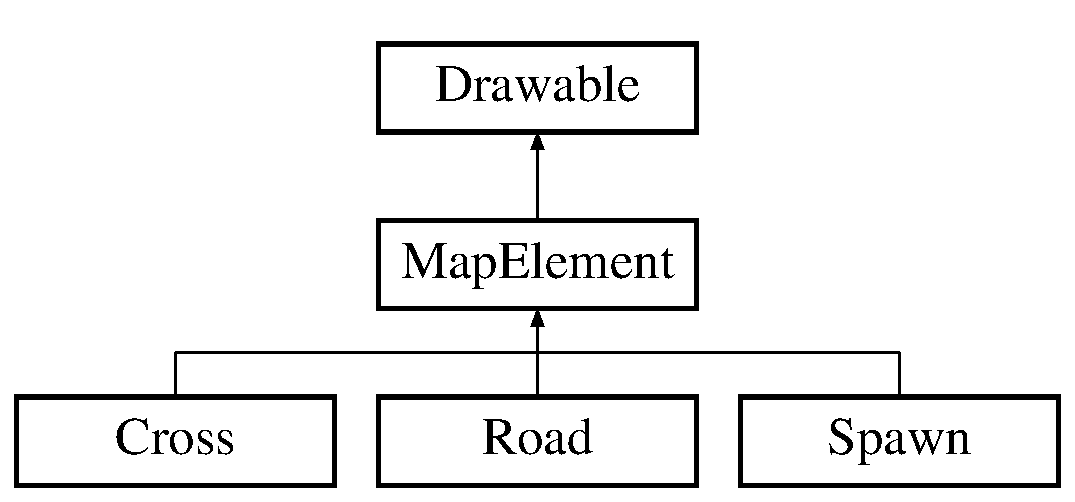
\includegraphics[height=3.000000cm]{class_map_element}
\end{center}
\end{figure}
\subsection*{Metody publiczne}
\begin{DoxyCompactItemize}
\item 
\hyperlink{class_map_element_a1e6c2dadb01e42de3980f1cb9a5e316c}{Map\-Element} ()
\begin{DoxyCompactList}\small\item\em Konstruktor. \end{DoxyCompactList}\item 
\hyperlink{class_map_element_abb9461a82f67bd340559879d305d3c43}{Map\-Element} (double x\-\_\-, double y\-\_\-, int id\-\_\-)
\begin{DoxyCompactList}\small\item\em Konstruktor. \end{DoxyCompactList}\item 
\hyperlink{class_map_element_a6eb24cff5179f6919b426ad3654545f1}{Map\-Element} (\hyperlink{struct_position}{Position} position\-\_\-, int id\-\_\-)
\begin{DoxyCompactList}\small\item\em Konstruktor. \end{DoxyCompactList}\item 
\hyperlink{class_map_element_a4e692e2575a667c25213e59d9ac893f7}{Map\-Element} (const \hyperlink{class_map_element}{Map\-Element} \&map\-Element)
\begin{DoxyCompactList}\small\item\em Konstruktor. \end{DoxyCompactList}\item 
virtual void \hyperlink{class_map_element_aa76ca7443c4f6a6683f68f44909b90d3}{draw} (\hyperlink{class_scene}{Scene} $\ast$scene)=0
\item 
int \hyperlink{class_map_element_a4b0a0465fb8859aa91ddb888857167bb}{get\-I\-D} () const 
\begin{DoxyCompactList}\small\item\em Metoda zwraca id elementu mapy. \end{DoxyCompactList}\item 
void \hyperlink{class_map_element_a616d51f35aba2279c6df5415f8ee29d9}{set\-I\-D} (const int id\-\_\-)
\begin{DoxyCompactList}\small\item\em Metoda ustawia id. \end{DoxyCompactList}\end{DoxyCompactItemize}
\subsection*{Atrybuty chronione}
\begin{DoxyCompactItemize}
\item 
int \hyperlink{class_map_element_a65ac80f170032e03dca2d2b751cbe688}{id}
\end{DoxyCompactItemize}


\subsection{Opis szczegółowy}
Klasa bazowa dla Drogi, Skrzyżowania i miejsc tworzenia pojazdów. 

\hyperlink{_map_element_8h}{Map\-Element.\-h} Klasa abstrakcyjna, bazowa dla wszystkich elementów mapy. 

\subsection{Dokumentacja konstruktora i destruktora}
\hypertarget{class_map_element_a1e6c2dadb01e42de3980f1cb9a5e316c}{\index{Map\-Element@{Map\-Element}!Map\-Element@{Map\-Element}}
\index{Map\-Element@{Map\-Element}!MapElement@{Map\-Element}}
\subsubsection[{Map\-Element}]{\setlength{\rightskip}{0pt plus 5cm}Map\-Element\-::\-Map\-Element (
\begin{DoxyParamCaption}
{}
\end{DoxyParamCaption}
)\hspace{0.3cm}{\ttfamily [inline]}}}\label{class_map_element_a1e6c2dadb01e42de3980f1cb9a5e316c}


Konstruktor. 

\hypertarget{class_map_element_abb9461a82f67bd340559879d305d3c43}{\index{Map\-Element@{Map\-Element}!Map\-Element@{Map\-Element}}
\index{Map\-Element@{Map\-Element}!MapElement@{Map\-Element}}
\subsubsection[{Map\-Element}]{\setlength{\rightskip}{0pt plus 5cm}Map\-Element\-::\-Map\-Element (
\begin{DoxyParamCaption}
\item[{double}]{x\-\_\-, }
\item[{double}]{y\-\_\-, }
\item[{int}]{id\-\_\-}
\end{DoxyParamCaption}
)\hspace{0.3cm}{\ttfamily [inline]}}}\label{class_map_element_abb9461a82f67bd340559879d305d3c43}


Konstruktor. 

\hypertarget{class_map_element_a6eb24cff5179f6919b426ad3654545f1}{\index{Map\-Element@{Map\-Element}!Map\-Element@{Map\-Element}}
\index{Map\-Element@{Map\-Element}!MapElement@{Map\-Element}}
\subsubsection[{Map\-Element}]{\setlength{\rightskip}{0pt plus 5cm}Map\-Element\-::\-Map\-Element (
\begin{DoxyParamCaption}
\item[{{\bf Position}}]{position\-\_\-, }
\item[{int}]{id\-\_\-}
\end{DoxyParamCaption}
)\hspace{0.3cm}{\ttfamily [inline]}}}\label{class_map_element_a6eb24cff5179f6919b426ad3654545f1}


Konstruktor. 

\hypertarget{class_map_element_a4e692e2575a667c25213e59d9ac893f7}{\index{Map\-Element@{Map\-Element}!Map\-Element@{Map\-Element}}
\index{Map\-Element@{Map\-Element}!MapElement@{Map\-Element}}
\subsubsection[{Map\-Element}]{\setlength{\rightskip}{0pt plus 5cm}Map\-Element\-::\-Map\-Element (
\begin{DoxyParamCaption}
\item[{const {\bf Map\-Element} \&}]{map\-Element}
\end{DoxyParamCaption}
)\hspace{0.3cm}{\ttfamily [inline]}}}\label{class_map_element_a4e692e2575a667c25213e59d9ac893f7}


Konstruktor. 



\subsection{Dokumentacja funkcji składowych}
\hypertarget{class_map_element_aa76ca7443c4f6a6683f68f44909b90d3}{\index{Map\-Element@{Map\-Element}!draw@{draw}}
\index{draw@{draw}!MapElement@{Map\-Element}}
\subsubsection[{draw}]{\setlength{\rightskip}{0pt plus 5cm}virtual void Map\-Element\-::draw (
\begin{DoxyParamCaption}
\item[{{\bf Scene} $\ast$}]{scene}
\end{DoxyParamCaption}
)\hspace{0.3cm}{\ttfamily [pure virtual]}}}\label{class_map_element_aa76ca7443c4f6a6683f68f44909b90d3}
To jest metoda przeciążona, udostępniona dla wygody. Różni się od powyższej metody tylko zestawem akceptowanych argumentów. 

Implementuje \hyperlink{class_drawable_a1e24b799e5b5f5494b25a42e2624692c}{Drawable}.



Implementowany w \hyperlink{class_cross_a3b127c19a196ad86bbd27b513eecdf44}{Cross}, \hyperlink{class_spawn_a725ac9cb33aff1b26b19ed3affecf692}{Spawn} i \hyperlink{class_road_a276332c2d6a617ca0fc665470fc49901}{Road}.

\hypertarget{class_map_element_a4b0a0465fb8859aa91ddb888857167bb}{\index{Map\-Element@{Map\-Element}!get\-I\-D@{get\-I\-D}}
\index{get\-I\-D@{get\-I\-D}!MapElement@{Map\-Element}}
\subsubsection[{get\-I\-D}]{\setlength{\rightskip}{0pt plus 5cm}int Map\-Element\-::get\-I\-D (
\begin{DoxyParamCaption}
{}
\end{DoxyParamCaption}
) const\hspace{0.3cm}{\ttfamily [inline]}}}\label{class_map_element_a4b0a0465fb8859aa91ddb888857167bb}


Metoda zwraca id elementu mapy. 

\hypertarget{class_map_element_a616d51f35aba2279c6df5415f8ee29d9}{\index{Map\-Element@{Map\-Element}!set\-I\-D@{set\-I\-D}}
\index{set\-I\-D@{set\-I\-D}!MapElement@{Map\-Element}}
\subsubsection[{set\-I\-D}]{\setlength{\rightskip}{0pt plus 5cm}void Map\-Element\-::set\-I\-D (
\begin{DoxyParamCaption}
\item[{const int}]{id\-\_\-}
\end{DoxyParamCaption}
)\hspace{0.3cm}{\ttfamily [inline]}}}\label{class_map_element_a616d51f35aba2279c6df5415f8ee29d9}


Metoda ustawia id. 



\subsection{Dokumentacja atrybutów składowych}
\hypertarget{class_map_element_a65ac80f170032e03dca2d2b751cbe688}{\index{Map\-Element@{Map\-Element}!id@{id}}
\index{id@{id}!MapElement@{Map\-Element}}
\subsubsection[{id}]{\setlength{\rightskip}{0pt plus 5cm}int Map\-Element\-::id\hspace{0.3cm}{\ttfamily [protected]}}}\label{class_map_element_a65ac80f170032e03dca2d2b751cbe688}


Dokumentacja dla tej klasy została wygenerowana z pliku\-:\begin{DoxyCompactItemize}
\item 
src/\hyperlink{_map_element_8h}{Map\-Element.\-h}\end{DoxyCompactItemize}

\hypertarget{class_map_exception}{\section{Dokumentacja klasy Map\-Exception}
\label{class_map_exception}\index{Map\-Exception@{Map\-Exception}}
}


Klasa wyjątku powstającego przy nieudanym tworzeniu mapy.  




{\ttfamily \#include $<$Exceptions.\-h$>$}

Diagram dziedziczenia dla Map\-Exception\begin{figure}[H]
\begin{center}
\leavevmode
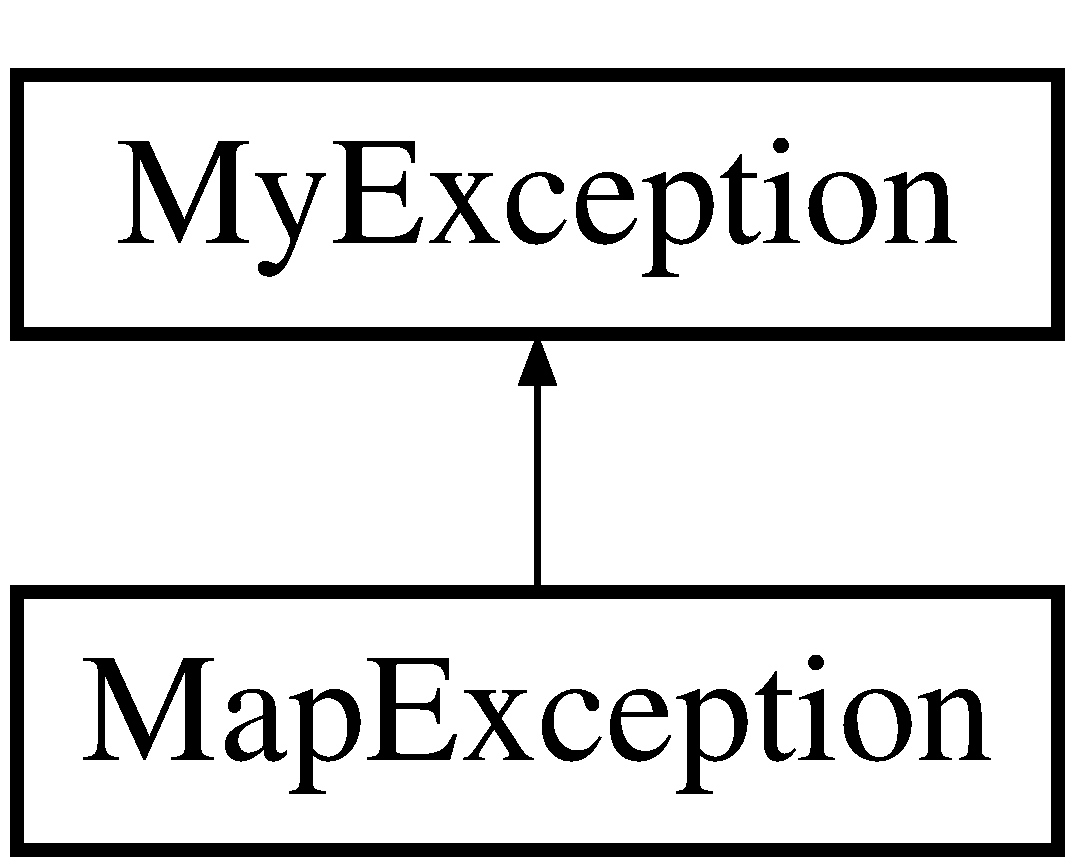
\includegraphics[height=2.000000cm]{class_map_exception}
\end{center}
\end{figure}
\subsection*{Metody publiczne}
\begin{DoxyCompactItemize}
\item 
\hyperlink{class_map_exception_a590408e1fea74604dbc156ba566a2436}{Map\-Exception} (string msg\-\_\-)
\item 
\hyperlink{class_map_exception_a98453a6aeae35b783a5f6a4ca1f6e842}{$\sim$\-Map\-Exception} ()  throw ()
\end{DoxyCompactItemize}
\subsection*{Dodatkowe Dziedziczone Składowe}


\subsection{Opis szczegółowy}
Klasa wyjątku powstającego przy nieudanym tworzeniu mapy. 

\subsection{Dokumentacja konstruktora i destruktora}
\hypertarget{class_map_exception_a590408e1fea74604dbc156ba566a2436}{\index{Map\-Exception@{Map\-Exception}!Map\-Exception@{Map\-Exception}}
\index{Map\-Exception@{Map\-Exception}!MapException@{Map\-Exception}}
\subsubsection[{Map\-Exception}]{\setlength{\rightskip}{0pt plus 5cm}Map\-Exception\-::\-Map\-Exception (
\begin{DoxyParamCaption}
\item[{string}]{msg\-\_\-}
\end{DoxyParamCaption}
)\hspace{0.3cm}{\ttfamily [inline]}}}\label{class_map_exception_a590408e1fea74604dbc156ba566a2436}
\hypertarget{class_map_exception_a98453a6aeae35b783a5f6a4ca1f6e842}{\index{Map\-Exception@{Map\-Exception}!$\sim$\-Map\-Exception@{$\sim$\-Map\-Exception}}
\index{$\sim$\-Map\-Exception@{$\sim$\-Map\-Exception}!MapException@{Map\-Exception}}
\subsubsection[{$\sim$\-Map\-Exception}]{\setlength{\rightskip}{0pt plus 5cm}Map\-Exception\-::$\sim$\-Map\-Exception (
\begin{DoxyParamCaption}
{}
\end{DoxyParamCaption}
)  throw ()\hspace{0.3cm}{\ttfamily [inline]}}}\label{class_map_exception_a98453a6aeae35b783a5f6a4ca1f6e842}


Dokumentacja dla tej klasy została wygenerowana z pliku\-:\begin{DoxyCompactItemize}
\item 
src/\hyperlink{_exceptions_8h}{Exceptions.\-h}\end{DoxyCompactItemize}

\hypertarget{class_map_factory}{\section{Dokumentacja klasy Map\-Factory}
\label{class_map_factory}\index{Map\-Factory@{Map\-Factory}}
}


Klasa odpowiada za czytanie pliku w formacie json i tworzenie na jego podstawie grafu i wszystkich elementów mapy.  




{\ttfamily \#include $<$Map\-Factory.\-h$>$}

\subsection*{Metody publiczne}
\begin{DoxyCompactItemize}
\item 
\hyperlink{class_map_factory_aad57a8dceca114847cc97579aaa6f569}{Map\-Factory} (const string \&)
\begin{DoxyCompactList}\small\item\em Konstruktor klasy \hyperlink{class_map_factory}{Map\-Factory}, parametrem jest scieżka do pliku. \end{DoxyCompactList}\item 
\hyperlink{_types_8h_adb8cbccb1bf63dda03515e30e185c388}{Graph} $\ast$ \hyperlink{class_map_factory_a22c43a80224a98a9ad11f9e38dcda29b}{create\-Map} ()
\begin{DoxyCompactList}\small\item\em Tworzy mapę i wszystkie elementy w niej zawarte. \end{DoxyCompactList}\item 
vector$<$ \hyperlink{_types_8h_a4260a5280323637f8a1fa28e89b6ef14}{P\-Map\-Element} $>$ \& \hyperlink{class_map_factory_a49c90b6c269407a3fc71d103edd6ff9e}{get\-Map\-Elements} ()
\begin{DoxyCompactList}\small\item\em Zwraca wektor zawierający elementy mapy. \end{DoxyCompactList}\item 
\hyperlink{class_map_factory_a21d7130504a10cc0886c26326b2faa9d}{$\sim$\-Map\-Factory} ()
\end{DoxyCompactItemize}
\subsection*{Metody prywatne}
\begin{DoxyCompactItemize}
\item 
void \hyperlink{class_map_factory_a64ee27fb682c6cc7b4c45dd856b8e607}{add\-Cross\-\_\-} (const ptree\-::value\-\_\-type \&)
\item 
void \hyperlink{class_map_factory_a443185cbfeddc063df6aed004d2c21fd}{add\-Spawn\-\_\-} (const ptree\-::value\-\_\-type \&)
\item 
void \hyperlink{class_map_factory_ac4bdddf0aeeaedae80a2cd8814aefd78}{add\-Edges\-\_\-} (int, map$<$ \hyperlink{_direction_8h_a224b9163917ac32fc95a60d8c1eec3aa}{Direction}, int $>$)
\item 
void \hyperlink{class_map_factory_addec2c9f5a0056a0887f09b781ffecf0}{add\-Edge\-\_\-} (int, int)
\end{DoxyCompactItemize}
\subsection*{Atrybuty prywatne}
\begin{DoxyCompactItemize}
\item 
\hyperlink{_types_8h_adb8cbccb1bf63dda03515e30e185c388}{Graph} $\ast$ \hyperlink{class_map_factory_af4450d69783b74d07d8686da50c66621}{g}
\item 
\hyperlink{_map_factory_8h_a54a98738cc1e3485f2cf5f24979317e5}{ptree} \hyperlink{class_map_factory_af0cbd48b8917121329660bd28877fcc6}{property\-Tree}
\item 
map$<$ int, \hyperlink{_types_8h_a8c93f604acf57e6a9bae1f91c379ac98}{Vertex} $>$ \hyperlink{class_map_factory_ab3f7a784d24d1cf06f03429312d030b4}{vertices}
\item 
map$<$ int, \hyperlink{_types_8h_a4260a5280323637f8a1fa28e89b6ef14}{P\-Map\-Element} $>$ \hyperlink{class_map_factory_aaf7d7680404bc0ac40766ca305f75753}{vertices\-Elements}
\item 
vector$<$ \hyperlink{_types_8h_a4260a5280323637f8a1fa28e89b6ef14}{P\-Map\-Element} $>$ \hyperlink{class_map_factory_ad4677e42d2e82c5ca31fa931fa60f9ce}{map\-Elements}
\end{DoxyCompactItemize}


\subsection{Opis szczegółowy}
Klasa odpowiada za czytanie pliku w formacie json i tworzenie na jego podstawie grafu i wszystkich elementów mapy. 

\subsection{Dokumentacja konstruktora i destruktora}
\hypertarget{class_map_factory_aad57a8dceca114847cc97579aaa6f569}{\index{Map\-Factory@{Map\-Factory}!Map\-Factory@{Map\-Factory}}
\index{Map\-Factory@{Map\-Factory}!MapFactory@{Map\-Factory}}
\subsubsection[{Map\-Factory}]{\setlength{\rightskip}{0pt plus 5cm}Map\-Factory\-::\-Map\-Factory (
\begin{DoxyParamCaption}
\item[{const string \&}]{path}
\end{DoxyParamCaption}
)}}\label{class_map_factory_aad57a8dceca114847cc97579aaa6f569}


Konstruktor klasy \hyperlink{class_map_factory}{Map\-Factory}, parametrem jest scieżka do pliku. 

\hypertarget{class_map_factory_a21d7130504a10cc0886c26326b2faa9d}{\index{Map\-Factory@{Map\-Factory}!$\sim$\-Map\-Factory@{$\sim$\-Map\-Factory}}
\index{$\sim$\-Map\-Factory@{$\sim$\-Map\-Factory}!MapFactory@{Map\-Factory}}
\subsubsection[{$\sim$\-Map\-Factory}]{\setlength{\rightskip}{0pt plus 5cm}Map\-Factory\-::$\sim$\-Map\-Factory (
\begin{DoxyParamCaption}
{}
\end{DoxyParamCaption}
)}}\label{class_map_factory_a21d7130504a10cc0886c26326b2faa9d}


\subsection{Dokumentacja funkcji składowych}
\hypertarget{class_map_factory_a64ee27fb682c6cc7b4c45dd856b8e607}{\index{Map\-Factory@{Map\-Factory}!add\-Cross\-\_\-@{add\-Cross\-\_\-}}
\index{add\-Cross\-\_\-@{add\-Cross\-\_\-}!MapFactory@{Map\-Factory}}
\subsubsection[{add\-Cross\-\_\-}]{\setlength{\rightskip}{0pt plus 5cm}void Map\-Factory\-::add\-Cross\-\_\- (
\begin{DoxyParamCaption}
\item[{const ptree\-::value\-\_\-type \&}]{v}
\end{DoxyParamCaption}
)\hspace{0.3cm}{\ttfamily [private]}}}\label{class_map_factory_a64ee27fb682c6cc7b4c45dd856b8e607}
\hypertarget{class_map_factory_addec2c9f5a0056a0887f09b781ffecf0}{\index{Map\-Factory@{Map\-Factory}!add\-Edge\-\_\-@{add\-Edge\-\_\-}}
\index{add\-Edge\-\_\-@{add\-Edge\-\_\-}!MapFactory@{Map\-Factory}}
\subsubsection[{add\-Edge\-\_\-}]{\setlength{\rightskip}{0pt plus 5cm}void Map\-Factory\-::add\-Edge\-\_\- (
\begin{DoxyParamCaption}
\item[{int}]{v1\-\_\-, }
\item[{int}]{v2\-\_\-}
\end{DoxyParamCaption}
)\hspace{0.3cm}{\ttfamily [private]}}}\label{class_map_factory_addec2c9f5a0056a0887f09b781ffecf0}
\hypertarget{class_map_factory_ac4bdddf0aeeaedae80a2cd8814aefd78}{\index{Map\-Factory@{Map\-Factory}!add\-Edges\-\_\-@{add\-Edges\-\_\-}}
\index{add\-Edges\-\_\-@{add\-Edges\-\_\-}!MapFactory@{Map\-Factory}}
\subsubsection[{add\-Edges\-\_\-}]{\setlength{\rightskip}{0pt plus 5cm}void Map\-Factory\-::add\-Edges\-\_\- (
\begin{DoxyParamCaption}
\item[{int}]{id\-\_\-, }
\item[{map$<$ {\bf Direction}, int $>$}]{neighbors\-\_\-}
\end{DoxyParamCaption}
)\hspace{0.3cm}{\ttfamily [private]}}}\label{class_map_factory_ac4bdddf0aeeaedae80a2cd8814aefd78}
\hypertarget{class_map_factory_a443185cbfeddc063df6aed004d2c21fd}{\index{Map\-Factory@{Map\-Factory}!add\-Spawn\-\_\-@{add\-Spawn\-\_\-}}
\index{add\-Spawn\-\_\-@{add\-Spawn\-\_\-}!MapFactory@{Map\-Factory}}
\subsubsection[{add\-Spawn\-\_\-}]{\setlength{\rightskip}{0pt plus 5cm}void Map\-Factory\-::add\-Spawn\-\_\- (
\begin{DoxyParamCaption}
\item[{const ptree\-::value\-\_\-type \&}]{v}
\end{DoxyParamCaption}
)\hspace{0.3cm}{\ttfamily [private]}}}\label{class_map_factory_a443185cbfeddc063df6aed004d2c21fd}
\hypertarget{class_map_factory_a22c43a80224a98a9ad11f9e38dcda29b}{\index{Map\-Factory@{Map\-Factory}!create\-Map@{create\-Map}}
\index{create\-Map@{create\-Map}!MapFactory@{Map\-Factory}}
\subsubsection[{create\-Map}]{\setlength{\rightskip}{0pt plus 5cm}{\bf Graph} $\ast$ Map\-Factory\-::create\-Map (
\begin{DoxyParamCaption}
{}
\end{DoxyParamCaption}
)}}\label{class_map_factory_a22c43a80224a98a9ad11f9e38dcda29b}


Tworzy mapę i wszystkie elementy w niej zawarte. 

\hypertarget{class_map_factory_a49c90b6c269407a3fc71d103edd6ff9e}{\index{Map\-Factory@{Map\-Factory}!get\-Map\-Elements@{get\-Map\-Elements}}
\index{get\-Map\-Elements@{get\-Map\-Elements}!MapFactory@{Map\-Factory}}
\subsubsection[{get\-Map\-Elements}]{\setlength{\rightskip}{0pt plus 5cm}vector$<$ {\bf P\-Map\-Element} $>$ \& Map\-Factory\-::get\-Map\-Elements (
\begin{DoxyParamCaption}
{}
\end{DoxyParamCaption}
)}}\label{class_map_factory_a49c90b6c269407a3fc71d103edd6ff9e}


Zwraca wektor zawierający elementy mapy. 



\subsection{Dokumentacja atrybutów składowych}
\hypertarget{class_map_factory_af4450d69783b74d07d8686da50c66621}{\index{Map\-Factory@{Map\-Factory}!g@{g}}
\index{g@{g}!MapFactory@{Map\-Factory}}
\subsubsection[{g}]{\setlength{\rightskip}{0pt plus 5cm}{\bf Graph}$\ast$ Map\-Factory\-::g\hspace{0.3cm}{\ttfamily [private]}}}\label{class_map_factory_af4450d69783b74d07d8686da50c66621}
\hypertarget{class_map_factory_ad4677e42d2e82c5ca31fa931fa60f9ce}{\index{Map\-Factory@{Map\-Factory}!map\-Elements@{map\-Elements}}
\index{map\-Elements@{map\-Elements}!MapFactory@{Map\-Factory}}
\subsubsection[{map\-Elements}]{\setlength{\rightskip}{0pt plus 5cm}vector$<${\bf P\-Map\-Element}$>$ Map\-Factory\-::map\-Elements\hspace{0.3cm}{\ttfamily [private]}}}\label{class_map_factory_ad4677e42d2e82c5ca31fa931fa60f9ce}
\hypertarget{class_map_factory_af0cbd48b8917121329660bd28877fcc6}{\index{Map\-Factory@{Map\-Factory}!property\-Tree@{property\-Tree}}
\index{property\-Tree@{property\-Tree}!MapFactory@{Map\-Factory}}
\subsubsection[{property\-Tree}]{\setlength{\rightskip}{0pt plus 5cm}{\bf ptree} Map\-Factory\-::property\-Tree\hspace{0.3cm}{\ttfamily [private]}}}\label{class_map_factory_af0cbd48b8917121329660bd28877fcc6}
\hypertarget{class_map_factory_ab3f7a784d24d1cf06f03429312d030b4}{\index{Map\-Factory@{Map\-Factory}!vertices@{vertices}}
\index{vertices@{vertices}!MapFactory@{Map\-Factory}}
\subsubsection[{vertices}]{\setlength{\rightskip}{0pt plus 5cm}map$<$int, {\bf Vertex}$>$ Map\-Factory\-::vertices\hspace{0.3cm}{\ttfamily [private]}}}\label{class_map_factory_ab3f7a784d24d1cf06f03429312d030b4}
\hypertarget{class_map_factory_aaf7d7680404bc0ac40766ca305f75753}{\index{Map\-Factory@{Map\-Factory}!vertices\-Elements@{vertices\-Elements}}
\index{vertices\-Elements@{vertices\-Elements}!MapFactory@{Map\-Factory}}
\subsubsection[{vertices\-Elements}]{\setlength{\rightskip}{0pt plus 5cm}map$<$int, {\bf P\-Map\-Element}$>$ Map\-Factory\-::vertices\-Elements\hspace{0.3cm}{\ttfamily [private]}}}\label{class_map_factory_aaf7d7680404bc0ac40766ca305f75753}


Dokumentacja dla tej klasy została wygenerowana z plików\-:\begin{DoxyCompactItemize}
\item 
src/\hyperlink{_map_factory_8h}{Map\-Factory.\-h}\item 
src/\hyperlink{_map_factory_8cpp}{Map\-Factory.\-cpp}\end{DoxyCompactItemize}

\hypertarget{class_moveable}{\section{Dokumentacja klasy Moveable}
\label{class_moveable}\index{Moveable@{Moveable}}
}


Klasa bazowa dla klas, które będą animowane.  




{\ttfamily \#include $<$Moveable.\-h$>$}

Diagram dziedziczenia dla Moveable\begin{figure}[H]
\begin{center}
\leavevmode
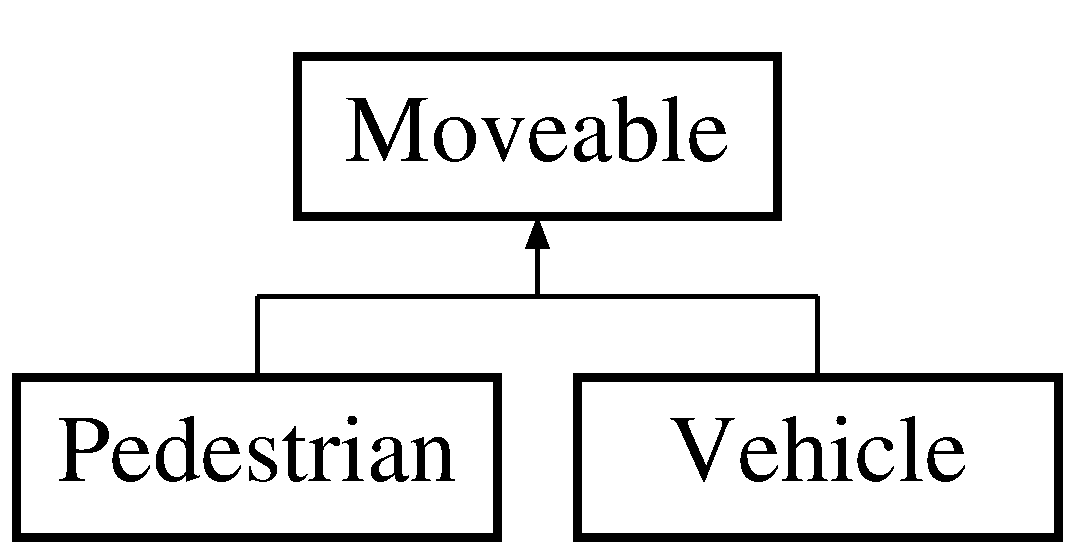
\includegraphics[height=2.000000cm]{class_moveable}
\end{center}
\end{figure}
\subsection*{Metody publiczne}
\begin{DoxyCompactItemize}
\item 
\hyperlink{class_moveable_ac76fdea840225276961ac42ba23e096e}{Moveable} (float max\-Speed\-\_\-, float acceleration\-\_\-)
\begin{DoxyCompactList}\small\item\em Konstruktor. \end{DoxyCompactList}\item 
virtual void \hyperlink{class_moveable_a3e42cec7b55d6320553b1c40e2392cb9}{calculate\-Position} ()=0
\begin{DoxyCompactList}\small\item\em Metoda obliczająca następną pozycję \end{DoxyCompactList}\item 
void \hyperlink{class_moveable_aa34a08ea960f6a48e1239861ba1442a1}{set\-Direction} (\hyperlink{_direction_8h_a224b9163917ac32fc95a60d8c1eec3aa}{Direction} d\-\_\-)
\begin{DoxyCompactList}\small\item\em Metoda ustawiająca kierunek ruchu. \end{DoxyCompactList}\end{DoxyCompactItemize}
\subsection*{Atrybuty chronione}
\begin{DoxyCompactItemize}
\item 
float \hyperlink{class_moveable_ab36dcef1bdc2dfdf662df044a61f7ba1}{max\-Speed}
\item 
float \hyperlink{class_moveable_a66d7998654c97643c5f95fdf26e886cf}{acceleration}
\item 
float \hyperlink{class_moveable_acbdd4bee0a3e3e9edffa29bb95d692fd}{current\-Speed}
\item 
double \hyperlink{class_moveable_ae84e95afddc19665f9fda53bfcd1c3a3}{dx}
\item 
double \hyperlink{class_moveable_ab110147d19762b3e03c9421a2232ae82}{dy}
\item 
\hyperlink{_direction_8h_a224b9163917ac32fc95a60d8c1eec3aa}{Direction} \hyperlink{class_moveable_a1bcc6c440945c5204b2819fe040e8396}{direction}
\item 
\hyperlink{_direction_8h_a224b9163917ac32fc95a60d8c1eec3aa}{Direction} \hyperlink{class_moveable_af654ea303b092f0e89a9bd81fd3c3ac0}{next\-Direction}
\end{DoxyCompactItemize}


\subsection{Opis szczegółowy}
Klasa bazowa dla klas, które będą animowane. 

\hyperlink{_moveable_8h}{Moveable.\-h} Author\-: Wookie 

\subsection{Dokumentacja konstruktora i destruktora}
\hypertarget{class_moveable_ac76fdea840225276961ac42ba23e096e}{\index{Moveable@{Moveable}!Moveable@{Moveable}}
\index{Moveable@{Moveable}!Moveable@{Moveable}}
\subsubsection[{Moveable}]{\setlength{\rightskip}{0pt plus 5cm}Moveable\-::\-Moveable (
\begin{DoxyParamCaption}
\item[{float}]{max\-Speed\-\_\-, }
\item[{float}]{acceleration\-\_\-}
\end{DoxyParamCaption}
)\hspace{0.3cm}{\ttfamily [inline]}}}\label{class_moveable_ac76fdea840225276961ac42ba23e096e}


Konstruktor. 



\subsection{Dokumentacja funkcji składowych}
\hypertarget{class_moveable_a3e42cec7b55d6320553b1c40e2392cb9}{\index{Moveable@{Moveable}!calculate\-Position@{calculate\-Position}}
\index{calculate\-Position@{calculate\-Position}!Moveable@{Moveable}}
\subsubsection[{calculate\-Position}]{\setlength{\rightskip}{0pt plus 5cm}virtual void Moveable\-::calculate\-Position (
\begin{DoxyParamCaption}
{}
\end{DoxyParamCaption}
)\hspace{0.3cm}{\ttfamily [pure virtual]}}}\label{class_moveable_a3e42cec7b55d6320553b1c40e2392cb9}


Metoda obliczająca następną pozycję 



Implementowany w \hyperlink{class_vehicle_ad5a55c6646313b8105b6dbb95b8eb89c}{Vehicle} i \hyperlink{class_pedestrian_aa7a2be507acde572507e185dc27eb6ec}{Pedestrian}.

\hypertarget{class_moveable_aa34a08ea960f6a48e1239861ba1442a1}{\index{Moveable@{Moveable}!set\-Direction@{set\-Direction}}
\index{set\-Direction@{set\-Direction}!Moveable@{Moveable}}
\subsubsection[{set\-Direction}]{\setlength{\rightskip}{0pt plus 5cm}void Moveable\-::set\-Direction (
\begin{DoxyParamCaption}
\item[{{\bf Direction}}]{d\-\_\-}
\end{DoxyParamCaption}
)\hspace{0.3cm}{\ttfamily [inline]}}}\label{class_moveable_aa34a08ea960f6a48e1239861ba1442a1}


Metoda ustawiająca kierunek ruchu. 



\subsection{Dokumentacja atrybutów składowych}
\hypertarget{class_moveable_a66d7998654c97643c5f95fdf26e886cf}{\index{Moveable@{Moveable}!acceleration@{acceleration}}
\index{acceleration@{acceleration}!Moveable@{Moveable}}
\subsubsection[{acceleration}]{\setlength{\rightskip}{0pt plus 5cm}float Moveable\-::acceleration\hspace{0.3cm}{\ttfamily [protected]}}}\label{class_moveable_a66d7998654c97643c5f95fdf26e886cf}
\hypertarget{class_moveable_acbdd4bee0a3e3e9edffa29bb95d692fd}{\index{Moveable@{Moveable}!current\-Speed@{current\-Speed}}
\index{current\-Speed@{current\-Speed}!Moveable@{Moveable}}
\subsubsection[{current\-Speed}]{\setlength{\rightskip}{0pt plus 5cm}float Moveable\-::current\-Speed\hspace{0.3cm}{\ttfamily [protected]}}}\label{class_moveable_acbdd4bee0a3e3e9edffa29bb95d692fd}
\hypertarget{class_moveable_a1bcc6c440945c5204b2819fe040e8396}{\index{Moveable@{Moveable}!direction@{direction}}
\index{direction@{direction}!Moveable@{Moveable}}
\subsubsection[{direction}]{\setlength{\rightskip}{0pt plus 5cm}{\bf Direction} Moveable\-::direction\hspace{0.3cm}{\ttfamily [protected]}}}\label{class_moveable_a1bcc6c440945c5204b2819fe040e8396}
\hypertarget{class_moveable_ae84e95afddc19665f9fda53bfcd1c3a3}{\index{Moveable@{Moveable}!dx@{dx}}
\index{dx@{dx}!Moveable@{Moveable}}
\subsubsection[{dx}]{\setlength{\rightskip}{0pt plus 5cm}double Moveable\-::dx\hspace{0.3cm}{\ttfamily [protected]}}}\label{class_moveable_ae84e95afddc19665f9fda53bfcd1c3a3}
\hypertarget{class_moveable_ab110147d19762b3e03c9421a2232ae82}{\index{Moveable@{Moveable}!dy@{dy}}
\index{dy@{dy}!Moveable@{Moveable}}
\subsubsection[{dy}]{\setlength{\rightskip}{0pt plus 5cm}double Moveable\-::dy\hspace{0.3cm}{\ttfamily [protected]}}}\label{class_moveable_ab110147d19762b3e03c9421a2232ae82}
\hypertarget{class_moveable_ab36dcef1bdc2dfdf662df044a61f7ba1}{\index{Moveable@{Moveable}!max\-Speed@{max\-Speed}}
\index{max\-Speed@{max\-Speed}!Moveable@{Moveable}}
\subsubsection[{max\-Speed}]{\setlength{\rightskip}{0pt plus 5cm}float Moveable\-::max\-Speed\hspace{0.3cm}{\ttfamily [protected]}}}\label{class_moveable_ab36dcef1bdc2dfdf662df044a61f7ba1}
\hypertarget{class_moveable_af654ea303b092f0e89a9bd81fd3c3ac0}{\index{Moveable@{Moveable}!next\-Direction@{next\-Direction}}
\index{next\-Direction@{next\-Direction}!Moveable@{Moveable}}
\subsubsection[{next\-Direction}]{\setlength{\rightskip}{0pt plus 5cm}{\bf Direction} Moveable\-::next\-Direction\hspace{0.3cm}{\ttfamily [protected]}}}\label{class_moveable_af654ea303b092f0e89a9bd81fd3c3ac0}


Dokumentacja dla tej klasy została wygenerowana z pliku\-:\begin{DoxyCompactItemize}
\item 
src/\hyperlink{_moveable_8h}{Moveable.\-h}\end{DoxyCompactItemize}

\hypertarget{class_my_exception}{\section{Dokumentacja klasy My\-Exception}
\label{class_my_exception}\index{My\-Exception@{My\-Exception}}
}


Klasa bazowa dla tworzonych w aplikacji wyjątków.  




{\ttfamily \#include $<$Exceptions.\-h$>$}

Diagram dziedziczenia dla My\-Exception\begin{figure}[H]
\begin{center}
\leavevmode
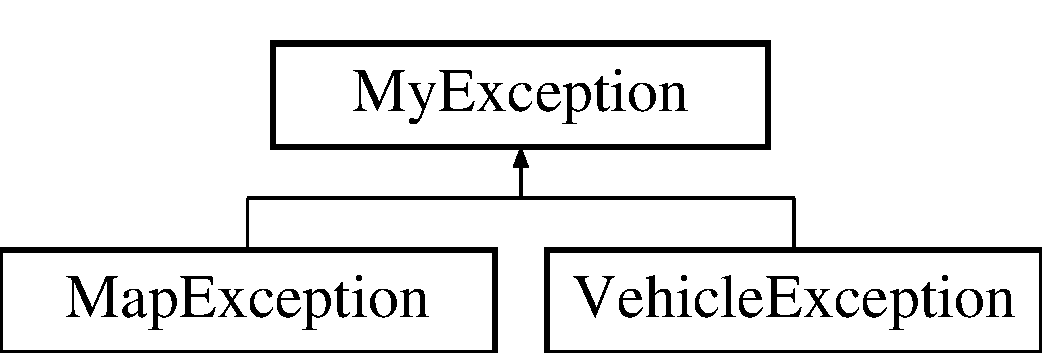
\includegraphics[height=2.000000cm]{class_my_exception}
\end{center}
\end{figure}
\subsection*{Metody publiczne}
\begin{DoxyCompactItemize}
\item 
\hyperlink{class_my_exception_abe961214430406426e1de998a7cc53e8}{My\-Exception} (string msg\-\_\-)
\begin{DoxyCompactList}\small\item\em Konstruktor. \end{DoxyCompactList}\item 
const string \& \hyperlink{class_my_exception_abba34689ff4de6027e6d9c765520ef49}{get\-Msg} ()
\begin{DoxyCompactList}\small\item\em Metoda zwraca wiadomość z wyjątku. \end{DoxyCompactList}\item 
\hyperlink{class_my_exception_aeb881435c0b8f981e04008795d4fde3b}{$\sim$\-My\-Exception} ()  throw ()
\end{DoxyCompactItemize}
\subsection*{Atrybuty chronione}
\begin{DoxyCompactItemize}
\item 
string \hyperlink{class_my_exception_ab8a915fca776573643452da65db7d3ed}{msg}
\end{DoxyCompactItemize}


\subsection{Opis szczegółowy}
Klasa bazowa dla tworzonych w aplikacji wyjątków. 

\subsection{Dokumentacja konstruktora i destruktora}
\hypertarget{class_my_exception_abe961214430406426e1de998a7cc53e8}{\index{My\-Exception@{My\-Exception}!My\-Exception@{My\-Exception}}
\index{My\-Exception@{My\-Exception}!MyException@{My\-Exception}}
\subsubsection[{My\-Exception}]{\setlength{\rightskip}{0pt plus 5cm}My\-Exception\-::\-My\-Exception (
\begin{DoxyParamCaption}
\item[{string}]{msg\-\_\-}
\end{DoxyParamCaption}
)\hspace{0.3cm}{\ttfamily [inline]}}}\label{class_my_exception_abe961214430406426e1de998a7cc53e8}


Konstruktor. 

\hypertarget{class_my_exception_aeb881435c0b8f981e04008795d4fde3b}{\index{My\-Exception@{My\-Exception}!$\sim$\-My\-Exception@{$\sim$\-My\-Exception}}
\index{$\sim$\-My\-Exception@{$\sim$\-My\-Exception}!MyException@{My\-Exception}}
\subsubsection[{$\sim$\-My\-Exception}]{\setlength{\rightskip}{0pt plus 5cm}My\-Exception\-::$\sim$\-My\-Exception (
\begin{DoxyParamCaption}
{}
\end{DoxyParamCaption}
)  throw ()\hspace{0.3cm}{\ttfamily [inline]}}}\label{class_my_exception_aeb881435c0b8f981e04008795d4fde3b}


\subsection{Dokumentacja funkcji składowych}
\hypertarget{class_my_exception_abba34689ff4de6027e6d9c765520ef49}{\index{My\-Exception@{My\-Exception}!get\-Msg@{get\-Msg}}
\index{get\-Msg@{get\-Msg}!MyException@{My\-Exception}}
\subsubsection[{get\-Msg}]{\setlength{\rightskip}{0pt plus 5cm}const string\& My\-Exception\-::get\-Msg (
\begin{DoxyParamCaption}
{}
\end{DoxyParamCaption}
)\hspace{0.3cm}{\ttfamily [inline]}}}\label{class_my_exception_abba34689ff4de6027e6d9c765520ef49}


Metoda zwraca wiadomość z wyjątku. 



\subsection{Dokumentacja atrybutów składowych}
\hypertarget{class_my_exception_ab8a915fca776573643452da65db7d3ed}{\index{My\-Exception@{My\-Exception}!msg@{msg}}
\index{msg@{msg}!MyException@{My\-Exception}}
\subsubsection[{msg}]{\setlength{\rightskip}{0pt plus 5cm}string My\-Exception\-::msg\hspace{0.3cm}{\ttfamily [protected]}}}\label{class_my_exception_ab8a915fca776573643452da65db7d3ed}


Dokumentacja dla tej klasy została wygenerowana z pliku\-:\begin{DoxyCompactItemize}
\item 
src/\hyperlink{_exceptions_8h}{Exceptions.\-h}\end{DoxyCompactItemize}

\hypertarget{class_pedestrian}{\section{Dokumentacja klasy Pedestrian}
\label{class_pedestrian}\index{Pedestrian@{Pedestrian}}
}


Klasa reprezentująca pieszego.  




{\ttfamily \#include $<$Pedestrian.\-h$>$}

Diagram dziedziczenia dla Pedestrian\begin{figure}[H]
\begin{center}
\leavevmode
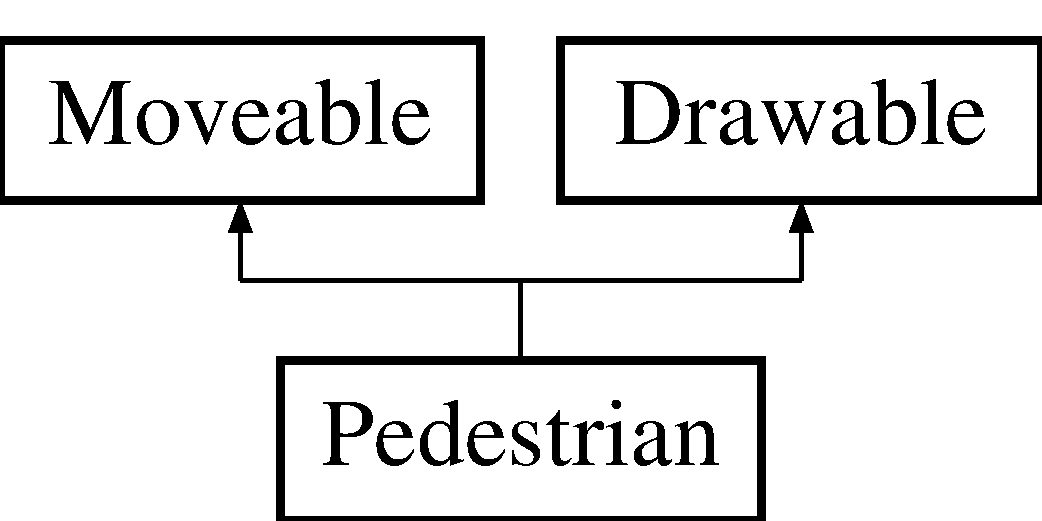
\includegraphics[height=2.000000cm]{class_pedestrian}
\end{center}
\end{figure}
\subsection*{Metody publiczne}
\begin{DoxyCompactItemize}
\item 
\hyperlink{class_pedestrian_acfccb3ad264cab78cf0efe3b2f1f9fc2}{Pedestrian} ()
\begin{DoxyCompactList}\small\item\em Konstruktor. \end{DoxyCompactList}\item 
virtual void \hyperlink{class_pedestrian_a51d926e2af8c607afef85f5e4d169a7a}{draw} (\hyperlink{class_scene}{Scene} $\ast$)
\item 
virtual void \hyperlink{class_pedestrian_aa7a2be507acde572507e185dc27eb6ec}{calculate\-Position} ()
\item 
void \hyperlink{class_pedestrian_ac53bd29d69fbe51c1d51064311ef36cc}{init} (\hyperlink{class_scene}{Scene} $\ast$)
\begin{DoxyCompactList}\small\item\em Metoda ustawia wszystkie początkowe wartości dla pieszego i dodaje Q\-Graphics\-Item do scene. \end{DoxyCompactList}\item 
void \hyperlink{class_pedestrian_a6244722d6aab61d21e2d1d9cd9152bd9}{update\-Q\-Item\-On\-Scene} ()
\begin{DoxyCompactList}\small\item\em Aktualizuje położenie q\-Item na scenie. \end{DoxyCompactList}\item 
void \hyperlink{class_pedestrian_a746a42831de03e17e5a15ab8066d14cf}{check\-Collisions} (\hyperlink{class_scene}{Scene} $\ast$)
\begin{DoxyCompactList}\small\item\em Sprawdza czy nastapiły kolizje z elementami mapy. \end{DoxyCompactList}\item 
bool \hyperlink{class_pedestrian_a74387251ec5d3eae4a14e5e87478282d}{is\-Not\-Active} () const 
\begin{DoxyCompactList}\small\item\em Zwraca true gdy pieszy jest niekatywny. \end{DoxyCompactList}\item 
virtual \hyperlink{class_pedestrian_af942446f2f37420c967fff3158e81e21}{$\sim$\-Pedestrian} ()
\end{DoxyCompactItemize}
\subsection*{Metody prywatne}
\begin{DoxyCompactItemize}
\item 
void \hyperlink{class_pedestrian_a3bdcdf87b8e1d416fbe07285a6ff3687}{check\-Collisions} ()
\item 
void \hyperlink{class_pedestrian_a3bbcc69a388edc3f89d3f4d81cde9707}{calculate\-Start\-Position} (\hyperlink{class_scene}{Scene} $\ast$)
\item 
void \hyperlink{class_pedestrian_adb3421e8cc94f890ef63d2c21f243241}{calculate\-Side} ()
\item 
bool \hyperlink{class_pedestrian_a6f9ed72743c2026b611dbdd2f9b519fb}{check\-Turn\-Position} ()
\end{DoxyCompactItemize}
\subsection*{Atrybuty prywatne}
\begin{DoxyCompactItemize}
\item 
Q\-Graphics\-Ellipse\-Item \hyperlink{class_pedestrian_a4f4897cab46bae56b3d4217167241ece}{q\-Item}
\item 
\hyperlink{class_cross}{Cross} $\ast$ \hyperlink{class_pedestrian_aaf596166aee518f9610d0b4ef724ff98}{cross}
\item 
int \hyperlink{class_pedestrian_a8b84bca49170ed2945b300e2cb430c27}{street\-Side}
\item 
Q\-Color \hyperlink{class_pedestrian_a4afcf22801bb0182dbdb30a9deb17247}{color}
\item 
vector$<$ \hyperlink{class_map_element}{Map\-Element} $\ast$ $>$ \hyperlink{class_pedestrian_a48bacc3e03bc81dde872f5673981a9cb}{collides\-Map\-Elements}
\end{DoxyCompactItemize}
\subsection*{Dodatkowe Dziedziczone Składowe}


\subsection{Opis szczegółowy}
Klasa reprezentująca pieszego. 

\subsection{Dokumentacja konstruktora i destruktora}
\hypertarget{class_pedestrian_acfccb3ad264cab78cf0efe3b2f1f9fc2}{\index{Pedestrian@{Pedestrian}!Pedestrian@{Pedestrian}}
\index{Pedestrian@{Pedestrian}!Pedestrian@{Pedestrian}}
\subsubsection[{Pedestrian}]{\setlength{\rightskip}{0pt plus 5cm}Pedestrian\-::\-Pedestrian (
\begin{DoxyParamCaption}
{}
\end{DoxyParamCaption}
)}}\label{class_pedestrian_acfccb3ad264cab78cf0efe3b2f1f9fc2}


Konstruktor. 

\hypertarget{class_pedestrian_af942446f2f37420c967fff3158e81e21}{\index{Pedestrian@{Pedestrian}!$\sim$\-Pedestrian@{$\sim$\-Pedestrian}}
\index{$\sim$\-Pedestrian@{$\sim$\-Pedestrian}!Pedestrian@{Pedestrian}}
\subsubsection[{$\sim$\-Pedestrian}]{\setlength{\rightskip}{0pt plus 5cm}Pedestrian\-::$\sim$\-Pedestrian (
\begin{DoxyParamCaption}
{}
\end{DoxyParamCaption}
)\hspace{0.3cm}{\ttfamily [virtual]}}}\label{class_pedestrian_af942446f2f37420c967fff3158e81e21}


\subsection{Dokumentacja funkcji składowych}
\hypertarget{class_pedestrian_aa7a2be507acde572507e185dc27eb6ec}{\index{Pedestrian@{Pedestrian}!calculate\-Position@{calculate\-Position}}
\index{calculate\-Position@{calculate\-Position}!Pedestrian@{Pedestrian}}
\subsubsection[{calculate\-Position}]{\setlength{\rightskip}{0pt plus 5cm}void Pedestrian\-::calculate\-Position (
\begin{DoxyParamCaption}
{}
\end{DoxyParamCaption}
)\hspace{0.3cm}{\ttfamily [virtual]}}}\label{class_pedestrian_aa7a2be507acde572507e185dc27eb6ec}
To jest metoda przeciążona, udostępniona dla wygody. Różni się od powyższej metody tylko zestawem akceptowanych argumentów. 

Implementuje \hyperlink{class_moveable_a3e42cec7b55d6320553b1c40e2392cb9}{Moveable}.

\hypertarget{class_pedestrian_adb3421e8cc94f890ef63d2c21f243241}{\index{Pedestrian@{Pedestrian}!calculate\-Side@{calculate\-Side}}
\index{calculate\-Side@{calculate\-Side}!Pedestrian@{Pedestrian}}
\subsubsection[{calculate\-Side}]{\setlength{\rightskip}{0pt plus 5cm}void Pedestrian\-::calculate\-Side (
\begin{DoxyParamCaption}
{}
\end{DoxyParamCaption}
)\hspace{0.3cm}{\ttfamily [private]}}}\label{class_pedestrian_adb3421e8cc94f890ef63d2c21f243241}
\hypertarget{class_pedestrian_a3bbcc69a388edc3f89d3f4d81cde9707}{\index{Pedestrian@{Pedestrian}!calculate\-Start\-Position@{calculate\-Start\-Position}}
\index{calculate\-Start\-Position@{calculate\-Start\-Position}!Pedestrian@{Pedestrian}}
\subsubsection[{calculate\-Start\-Position}]{\setlength{\rightskip}{0pt plus 5cm}void Pedestrian\-::calculate\-Start\-Position (
\begin{DoxyParamCaption}
\item[{{\bf Scene} $\ast$}]{scene\-\_\-}
\end{DoxyParamCaption}
)\hspace{0.3cm}{\ttfamily [private]}}}\label{class_pedestrian_a3bbcc69a388edc3f89d3f4d81cde9707}
\hypertarget{class_pedestrian_a3bdcdf87b8e1d416fbe07285a6ff3687}{\index{Pedestrian@{Pedestrian}!check\-Collisions@{check\-Collisions}}
\index{check\-Collisions@{check\-Collisions}!Pedestrian@{Pedestrian}}
\subsubsection[{check\-Collisions}]{\setlength{\rightskip}{0pt plus 5cm}void Pedestrian\-::check\-Collisions (
\begin{DoxyParamCaption}
{}
\end{DoxyParamCaption}
)\hspace{0.3cm}{\ttfamily [private]}}}\label{class_pedestrian_a3bdcdf87b8e1d416fbe07285a6ff3687}
\hypertarget{class_pedestrian_a746a42831de03e17e5a15ab8066d14cf}{\index{Pedestrian@{Pedestrian}!check\-Collisions@{check\-Collisions}}
\index{check\-Collisions@{check\-Collisions}!Pedestrian@{Pedestrian}}
\subsubsection[{check\-Collisions}]{\setlength{\rightskip}{0pt plus 5cm}void Pedestrian\-::check\-Collisions (
\begin{DoxyParamCaption}
\item[{{\bf Scene} $\ast$}]{scene\-\_\-}
\end{DoxyParamCaption}
)}}\label{class_pedestrian_a746a42831de03e17e5a15ab8066d14cf}


Sprawdza czy nastapiły kolizje z elementami mapy. 

\hypertarget{class_pedestrian_a6f9ed72743c2026b611dbdd2f9b519fb}{\index{Pedestrian@{Pedestrian}!check\-Turn\-Position@{check\-Turn\-Position}}
\index{check\-Turn\-Position@{check\-Turn\-Position}!Pedestrian@{Pedestrian}}
\subsubsection[{check\-Turn\-Position}]{\setlength{\rightskip}{0pt plus 5cm}bool Pedestrian\-::check\-Turn\-Position (
\begin{DoxyParamCaption}
{}
\end{DoxyParamCaption}
)\hspace{0.3cm}{\ttfamily [private]}}}\label{class_pedestrian_a6f9ed72743c2026b611dbdd2f9b519fb}
\hypertarget{class_pedestrian_a51d926e2af8c607afef85f5e4d169a7a}{\index{Pedestrian@{Pedestrian}!draw@{draw}}
\index{draw@{draw}!Pedestrian@{Pedestrian}}
\subsubsection[{draw}]{\setlength{\rightskip}{0pt plus 5cm}void Pedestrian\-::draw (
\begin{DoxyParamCaption}
\item[{{\bf Scene} $\ast$}]{}
\end{DoxyParamCaption}
)\hspace{0.3cm}{\ttfamily [virtual]}}}\label{class_pedestrian_a51d926e2af8c607afef85f5e4d169a7a}
To jest metoda przeciążona, udostępniona dla wygody. Różni się od powyższej metody tylko zestawem akceptowanych argumentów. 

Implementuje \hyperlink{class_drawable_a1e24b799e5b5f5494b25a42e2624692c}{Drawable}.

\hypertarget{class_pedestrian_ac53bd29d69fbe51c1d51064311ef36cc}{\index{Pedestrian@{Pedestrian}!init@{init}}
\index{init@{init}!Pedestrian@{Pedestrian}}
\subsubsection[{init}]{\setlength{\rightskip}{0pt plus 5cm}void Pedestrian\-::init (
\begin{DoxyParamCaption}
\item[{{\bf Scene} $\ast$}]{scene\-\_\-}
\end{DoxyParamCaption}
)}}\label{class_pedestrian_ac53bd29d69fbe51c1d51064311ef36cc}


Metoda ustawia wszystkie początkowe wartości dla pieszego i dodaje Q\-Graphics\-Item do scene. 

\hypertarget{class_pedestrian_a74387251ec5d3eae4a14e5e87478282d}{\index{Pedestrian@{Pedestrian}!is\-Not\-Active@{is\-Not\-Active}}
\index{is\-Not\-Active@{is\-Not\-Active}!Pedestrian@{Pedestrian}}
\subsubsection[{is\-Not\-Active}]{\setlength{\rightskip}{0pt plus 5cm}bool Pedestrian\-::is\-Not\-Active (
\begin{DoxyParamCaption}
{}
\end{DoxyParamCaption}
) const}}\label{class_pedestrian_a74387251ec5d3eae4a14e5e87478282d}


Zwraca true gdy pieszy jest niekatywny. 

\hypertarget{class_pedestrian_a6244722d6aab61d21e2d1d9cd9152bd9}{\index{Pedestrian@{Pedestrian}!update\-Q\-Item\-On\-Scene@{update\-Q\-Item\-On\-Scene}}
\index{update\-Q\-Item\-On\-Scene@{update\-Q\-Item\-On\-Scene}!Pedestrian@{Pedestrian}}
\subsubsection[{update\-Q\-Item\-On\-Scene}]{\setlength{\rightskip}{0pt plus 5cm}void Pedestrian\-::update\-Q\-Item\-On\-Scene (
\begin{DoxyParamCaption}
{}
\end{DoxyParamCaption}
)}}\label{class_pedestrian_a6244722d6aab61d21e2d1d9cd9152bd9}


Aktualizuje położenie q\-Item na scenie. 



\subsection{Dokumentacja atrybutów składowych}
\hypertarget{class_pedestrian_a48bacc3e03bc81dde872f5673981a9cb}{\index{Pedestrian@{Pedestrian}!collides\-Map\-Elements@{collides\-Map\-Elements}}
\index{collides\-Map\-Elements@{collides\-Map\-Elements}!Pedestrian@{Pedestrian}}
\subsubsection[{collides\-Map\-Elements}]{\setlength{\rightskip}{0pt plus 5cm}vector$<${\bf Map\-Element}$\ast$$>$ Pedestrian\-::collides\-Map\-Elements\hspace{0.3cm}{\ttfamily [private]}}}\label{class_pedestrian_a48bacc3e03bc81dde872f5673981a9cb}
\hypertarget{class_pedestrian_a4afcf22801bb0182dbdb30a9deb17247}{\index{Pedestrian@{Pedestrian}!color@{color}}
\index{color@{color}!Pedestrian@{Pedestrian}}
\subsubsection[{color}]{\setlength{\rightskip}{0pt plus 5cm}Q\-Color Pedestrian\-::color\hspace{0.3cm}{\ttfamily [private]}}}\label{class_pedestrian_a4afcf22801bb0182dbdb30a9deb17247}
\hypertarget{class_pedestrian_aaf596166aee518f9610d0b4ef724ff98}{\index{Pedestrian@{Pedestrian}!cross@{cross}}
\index{cross@{cross}!Pedestrian@{Pedestrian}}
\subsubsection[{cross}]{\setlength{\rightskip}{0pt plus 5cm}{\bf Cross}$\ast$ Pedestrian\-::cross\hspace{0.3cm}{\ttfamily [private]}}}\label{class_pedestrian_aaf596166aee518f9610d0b4ef724ff98}
\hypertarget{class_pedestrian_a4f4897cab46bae56b3d4217167241ece}{\index{Pedestrian@{Pedestrian}!q\-Item@{q\-Item}}
\index{q\-Item@{q\-Item}!Pedestrian@{Pedestrian}}
\subsubsection[{q\-Item}]{\setlength{\rightskip}{0pt plus 5cm}Q\-Graphics\-Ellipse\-Item Pedestrian\-::q\-Item\hspace{0.3cm}{\ttfamily [private]}}}\label{class_pedestrian_a4f4897cab46bae56b3d4217167241ece}
\hypertarget{class_pedestrian_a8b84bca49170ed2945b300e2cb430c27}{\index{Pedestrian@{Pedestrian}!street\-Side@{street\-Side}}
\index{street\-Side@{street\-Side}!Pedestrian@{Pedestrian}}
\subsubsection[{street\-Side}]{\setlength{\rightskip}{0pt plus 5cm}int Pedestrian\-::street\-Side\hspace{0.3cm}{\ttfamily [private]}}}\label{class_pedestrian_a8b84bca49170ed2945b300e2cb430c27}


Dokumentacja dla tej klasy została wygenerowana z plików\-:\begin{DoxyCompactItemize}
\item 
src/\hyperlink{_pedestrian_8h}{Pedestrian.\-h}\item 
src/\hyperlink{_pedestrian_8cpp}{Pedestrian.\-cpp}\end{DoxyCompactItemize}

\hypertarget{struct_position}{\section{Dokumentacja struktury Position}
\label{struct_position}\index{Position@{Position}}
}


Klasa reprezentuje punkt w trójwymiarowej przestrzeni.  




{\ttfamily \#include $<$Position.\-h$>$}

\subsection*{Metody publiczne}
\begin{DoxyCompactItemize}
\item 
\hyperlink{struct_position_ae4b5a0536e6c0dab44457ff34b21ac50}{Position} (double x\-\_\-, double y\-\_\-, double z\-\_\-=0)
\item 
\hyperlink{struct_position_a46126c3ef1893b4581e4726ac33b557b}{Position} (const \hyperlink{struct_position}{Position} \&position\-\_\-)
\item 
double \hyperlink{struct_position_a29f0bd21850b275c2c107e8a238979db}{abs\-X} () const 
\item 
double \hyperlink{struct_position_a7c8267cc217b805e86691556f2232619}{abs\-Y} () const 
\item 
double \hyperlink{struct_position_a0176fb7d30f2fbb8cf8d4ba1242a4610}{abs\-Z} () const 
\end{DoxyCompactItemize}
\subsection*{Atrybuty publiczne}
\begin{DoxyCompactItemize}
\item 
double \hyperlink{struct_position_a9abbe738bad177de91fe4774099c1260}{x}
\item 
double \hyperlink{struct_position_a75f48c2a1d2c7131b8be1a0687ae72c8}{y}
\item 
double \hyperlink{struct_position_ab26043bc2f8f6094818c17dd44e43228}{z}
\end{DoxyCompactItemize}


\subsection{Opis szczegółowy}
Klasa reprezentuje punkt w trójwymiarowej przestrzeni. 

\subsection{Dokumentacja konstruktora i destruktora}
\hypertarget{struct_position_ae4b5a0536e6c0dab44457ff34b21ac50}{\index{Position@{Position}!Position@{Position}}
\index{Position@{Position}!Position@{Position}}
\subsubsection[{Position}]{\setlength{\rightskip}{0pt plus 5cm}Position\-::\-Position (
\begin{DoxyParamCaption}
\item[{double}]{x\-\_\-, }
\item[{double}]{y\-\_\-, }
\item[{double}]{z\-\_\- = {\ttfamily 0}}
\end{DoxyParamCaption}
)\hspace{0.3cm}{\ttfamily [inline]}}}\label{struct_position_ae4b5a0536e6c0dab44457ff34b21ac50}
\hypertarget{struct_position_a46126c3ef1893b4581e4726ac33b557b}{\index{Position@{Position}!Position@{Position}}
\index{Position@{Position}!Position@{Position}}
\subsubsection[{Position}]{\setlength{\rightskip}{0pt plus 5cm}Position\-::\-Position (
\begin{DoxyParamCaption}
\item[{const {\bf Position} \&}]{position\-\_\-}
\end{DoxyParamCaption}
)\hspace{0.3cm}{\ttfamily [inline]}}}\label{struct_position_a46126c3ef1893b4581e4726ac33b557b}


\subsection{Dokumentacja funkcji składowych}
\hypertarget{struct_position_a29f0bd21850b275c2c107e8a238979db}{\index{Position@{Position}!abs\-X@{abs\-X}}
\index{abs\-X@{abs\-X}!Position@{Position}}
\subsubsection[{abs\-X}]{\setlength{\rightskip}{0pt plus 5cm}double Position\-::abs\-X (
\begin{DoxyParamCaption}
{}
\end{DoxyParamCaption}
) const\hspace{0.3cm}{\ttfamily [inline]}}}\label{struct_position_a29f0bd21850b275c2c107e8a238979db}
\hypertarget{struct_position_a7c8267cc217b805e86691556f2232619}{\index{Position@{Position}!abs\-Y@{abs\-Y}}
\index{abs\-Y@{abs\-Y}!Position@{Position}}
\subsubsection[{abs\-Y}]{\setlength{\rightskip}{0pt plus 5cm}double Position\-::abs\-Y (
\begin{DoxyParamCaption}
{}
\end{DoxyParamCaption}
) const\hspace{0.3cm}{\ttfamily [inline]}}}\label{struct_position_a7c8267cc217b805e86691556f2232619}
\hypertarget{struct_position_a0176fb7d30f2fbb8cf8d4ba1242a4610}{\index{Position@{Position}!abs\-Z@{abs\-Z}}
\index{abs\-Z@{abs\-Z}!Position@{Position}}
\subsubsection[{abs\-Z}]{\setlength{\rightskip}{0pt plus 5cm}double Position\-::abs\-Z (
\begin{DoxyParamCaption}
{}
\end{DoxyParamCaption}
) const\hspace{0.3cm}{\ttfamily [inline]}}}\label{struct_position_a0176fb7d30f2fbb8cf8d4ba1242a4610}


\subsection{Dokumentacja atrybutów składowych}
\hypertarget{struct_position_a9abbe738bad177de91fe4774099c1260}{\index{Position@{Position}!x@{x}}
\index{x@{x}!Position@{Position}}
\subsubsection[{x}]{\setlength{\rightskip}{0pt plus 5cm}double Position\-::x}}\label{struct_position_a9abbe738bad177de91fe4774099c1260}
\hypertarget{struct_position_a75f48c2a1d2c7131b8be1a0687ae72c8}{\index{Position@{Position}!y@{y}}
\index{y@{y}!Position@{Position}}
\subsubsection[{y}]{\setlength{\rightskip}{0pt plus 5cm}double Position\-::y}}\label{struct_position_a75f48c2a1d2c7131b8be1a0687ae72c8}
\hypertarget{struct_position_ab26043bc2f8f6094818c17dd44e43228}{\index{Position@{Position}!z@{z}}
\index{z@{z}!Position@{Position}}
\subsubsection[{z}]{\setlength{\rightskip}{0pt plus 5cm}double Position\-::z}}\label{struct_position_ab26043bc2f8f6094818c17dd44e43228}


Dokumentacja dla tej struktury została wygenerowana z pliku\-:\begin{DoxyCompactItemize}
\item 
src/\hyperlink{_position_8h}{Position.\-h}\end{DoxyCompactItemize}

\hypertarget{class_priority_rules}{\section{Dokumentacja klasy Priority\-Rules}
\label{class_priority_rules}\index{Priority\-Rules@{Priority\-Rules}}
}


Klasa bazowa dla \hyperlink{class_cross_rules}{Cross\-Rules}. Dwustopniowa herarchia klas umożliwia późniejszy rozwój. Np. dodanie sygnalizacji świetlnej.  




{\ttfamily \#include $<$Priority\-Rules.\-h$>$}

Diagram dziedziczenia dla Priority\-Rules\begin{figure}[H]
\begin{center}
\leavevmode
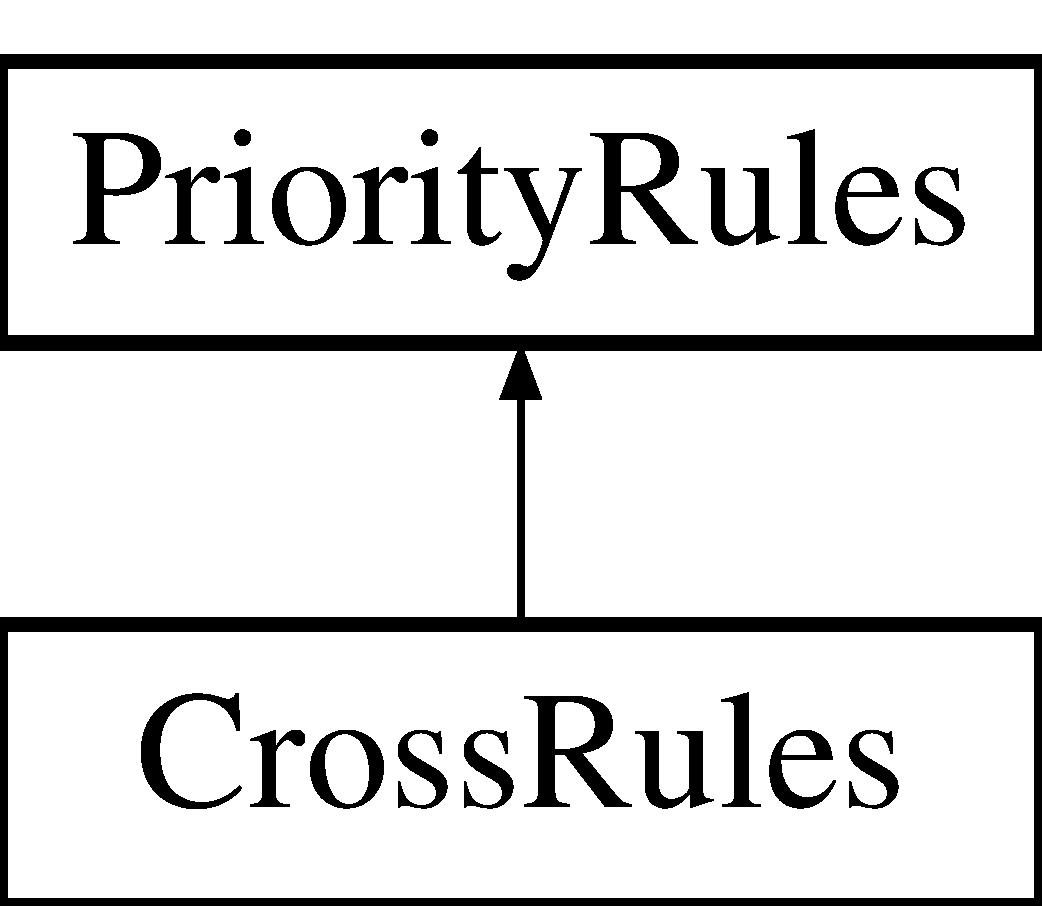
\includegraphics[height=2.000000cm]{class_priority_rules}
\end{center}
\end{figure}
\subsection*{Metody publiczne}
\begin{DoxyCompactItemize}
\item 
\hyperlink{class_priority_rules_a24de628b797363cfed852a507bb36291}{Priority\-Rules} ()
\item 
virtual std\-::set$<$ \hyperlink{_direction_8h_a224b9163917ac32fc95a60d8c1eec3aa}{Direction} $>$ \hyperlink{class_priority_rules_a1a64b70868b8c50ebe6bbc01062da361}{get\-Rules} (\hyperlink{_direction_8h_a224b9163917ac32fc95a60d8c1eec3aa}{Direction}, \hyperlink{_direction_8h_a224b9163917ac32fc95a60d8c1eec3aa}{Direction})=0
\end{DoxyCompactItemize}


\subsection{Opis szczegółowy}
Klasa bazowa dla \hyperlink{class_cross_rules}{Cross\-Rules}. Dwustopniowa herarchia klas umożliwia późniejszy rozwój. Np. dodanie sygnalizacji świetlnej. 

\hyperlink{_priority_rules_8h}{Priority\-Rules.\-h} Klasa bazowa dla wszystkich systemów obsługi pierwszeństwa przejazdu na skrzyżowaniach (np. zwykłe reguły pierwszeństwa, sygnalizacja świetlna). 

\subsection{Dokumentacja konstruktora i destruktora}
\hypertarget{class_priority_rules_a24de628b797363cfed852a507bb36291}{\index{Priority\-Rules@{Priority\-Rules}!Priority\-Rules@{Priority\-Rules}}
\index{Priority\-Rules@{Priority\-Rules}!PriorityRules@{Priority\-Rules}}
\subsubsection[{Priority\-Rules}]{\setlength{\rightskip}{0pt plus 5cm}Priority\-Rules\-::\-Priority\-Rules (
\begin{DoxyParamCaption}
{}
\end{DoxyParamCaption}
)\hspace{0.3cm}{\ttfamily [inline]}}}\label{class_priority_rules_a24de628b797363cfed852a507bb36291}


\subsection{Dokumentacja funkcji składowych}
\hypertarget{class_priority_rules_a1a64b70868b8c50ebe6bbc01062da361}{\index{Priority\-Rules@{Priority\-Rules}!get\-Rules@{get\-Rules}}
\index{get\-Rules@{get\-Rules}!PriorityRules@{Priority\-Rules}}
\subsubsection[{get\-Rules}]{\setlength{\rightskip}{0pt plus 5cm}virtual std\-::set$<${\bf Direction}$>$ Priority\-Rules\-::get\-Rules (
\begin{DoxyParamCaption}
\item[{{\bf Direction}}]{, }
\item[{{\bf Direction}}]{}
\end{DoxyParamCaption}
)\hspace{0.3cm}{\ttfamily [pure virtual]}}}\label{class_priority_rules_a1a64b70868b8c50ebe6bbc01062da361}


Implementowany w \hyperlink{class_cross_rules_afc553f8d0a643382b188ebd95faca30f}{Cross\-Rules}.



Dokumentacja dla tej klasy została wygenerowana z pliku\-:\begin{DoxyCompactItemize}
\item 
src/\hyperlink{_priority_rules_8h}{Priority\-Rules.\-h}\end{DoxyCompactItemize}

\hypertarget{class_road}{\section{Dokumentacja klasy Road}
\label{class_road}\index{Road@{Road}}
}


Klasa reprezentuje drogę na mapie.  




{\ttfamily \#include $<$Road.\-h$>$}

Diagram dziedziczenia dla Road\begin{figure}[H]
\begin{center}
\leavevmode
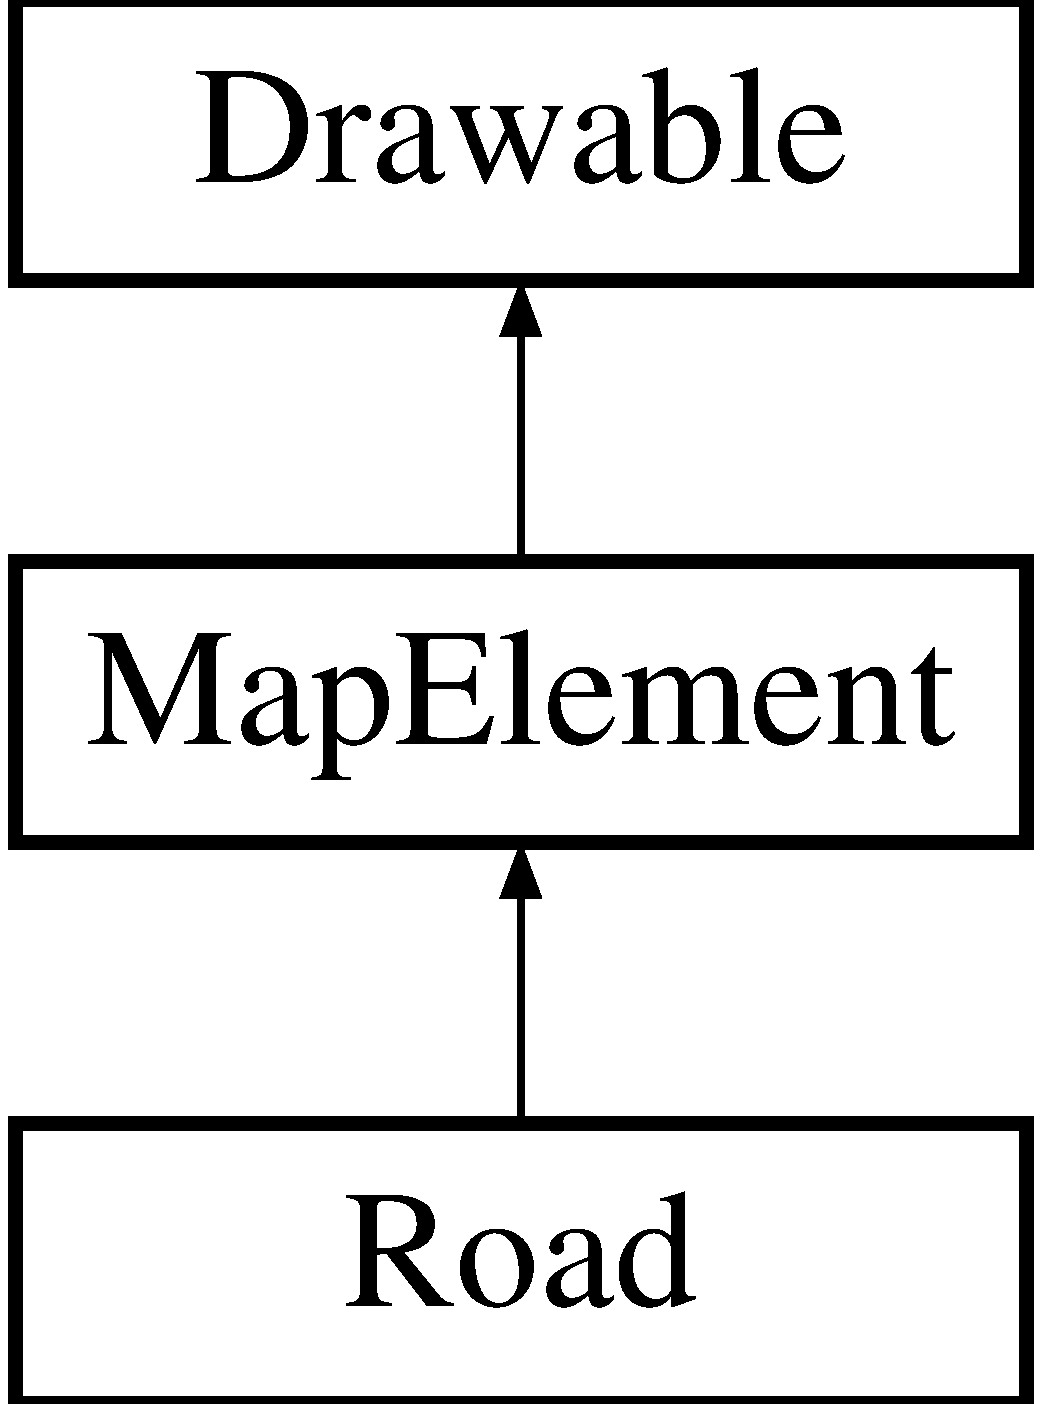
\includegraphics[height=3.000000cm]{class_road}
\end{center}
\end{figure}
\subsection*{Metody publiczne}
\begin{DoxyCompactItemize}
\item 
\hyperlink{class_road_a90bb6be2a5c3b6997849a915e2af0cf0}{Road} ()
\begin{DoxyCompactList}\small\item\em Konstruktor. \end{DoxyCompactList}\item 
\hyperlink{class_road_a65e61485d6940225dbdb9f6def8e6aa4}{Road} (\hyperlink{_types_8h_a4260a5280323637f8a1fa28e89b6ef14}{P\-Map\-Element} from\-\_\-, \hyperlink{_types_8h_a4260a5280323637f8a1fa28e89b6ef14}{P\-Map\-Element} to\-\_\-)
\item 
virtual void \hyperlink{class_road_a276332c2d6a617ca0fc665470fc49901}{draw} (\hyperlink{class_scene}{Scene} $\ast$scene)
\begin{DoxyCompactList}\small\item\em Metoda tworząca i dodająca obiekty Graphics\-Item do sceny. \end{DoxyCompactList}\item 
int \hyperlink{class_road_ac28b45b44c84944d22aa737fc53a45af}{get\-Length} () const 
\begin{DoxyCompactList}\small\item\em Zwraca długość drogi. \end{DoxyCompactList}\item 
virtual \hyperlink{class_road_ab32a196528ec20e7665a0c402a241b4e}{$\sim$\-Road} ()
\end{DoxyCompactItemize}
\subsection*{Atrybuty prywatne}
\begin{DoxyCompactItemize}
\item 
\hyperlink{_direction_8h_a224b9163917ac32fc95a60d8c1eec3aa}{Direction} \hyperlink{class_road_a751b38c96aad271b5e1ac771f82059d1}{direction}
\item 
int \hyperlink{class_road_ad255cda1be7acc3806c8946154e9f79f}{length}
\item 
\hyperlink{_types_8h_a4260a5280323637f8a1fa28e89b6ef14}{P\-Map\-Element} \hyperlink{class_road_acf1b7cd300df6c8617e6f0fe68c9f688}{from}
\item 
\hyperlink{_types_8h_a4260a5280323637f8a1fa28e89b6ef14}{P\-Map\-Element} \hyperlink{class_road_acdc9a6cb99fa3e7fb4042560d143bb53}{to}
\end{DoxyCompactItemize}
\subsection*{Dodatkowe Dziedziczone Składowe}


\subsection{Opis szczegółowy}
Klasa reprezentuje drogę na mapie. 

\subsection{Dokumentacja konstruktora i destruktora}
\hypertarget{class_road_a90bb6be2a5c3b6997849a915e2af0cf0}{\index{Road@{Road}!Road@{Road}}
\index{Road@{Road}!Road@{Road}}
\subsubsection[{Road}]{\setlength{\rightskip}{0pt plus 5cm}Road\-::\-Road (
\begin{DoxyParamCaption}
{}
\end{DoxyParamCaption}
)\hspace{0.3cm}{\ttfamily [inline]}}}\label{class_road_a90bb6be2a5c3b6997849a915e2af0cf0}


Konstruktor. 

\hypertarget{class_road_a65e61485d6940225dbdb9f6def8e6aa4}{\index{Road@{Road}!Road@{Road}}
\index{Road@{Road}!Road@{Road}}
\subsubsection[{Road}]{\setlength{\rightskip}{0pt plus 5cm}Road\-::\-Road (
\begin{DoxyParamCaption}
\item[{{\bf P\-Map\-Element}}]{from\-\_\-, }
\item[{{\bf P\-Map\-Element}}]{to\-\_\-}
\end{DoxyParamCaption}
)}}\label{class_road_a65e61485d6940225dbdb9f6def8e6aa4}
\hypertarget{class_road_ab32a196528ec20e7665a0c402a241b4e}{\index{Road@{Road}!$\sim$\-Road@{$\sim$\-Road}}
\index{$\sim$\-Road@{$\sim$\-Road}!Road@{Road}}
\subsubsection[{$\sim$\-Road}]{\setlength{\rightskip}{0pt plus 5cm}virtual Road\-::$\sim$\-Road (
\begin{DoxyParamCaption}
{}
\end{DoxyParamCaption}
)\hspace{0.3cm}{\ttfamily [inline]}, {\ttfamily [virtual]}}}\label{class_road_ab32a196528ec20e7665a0c402a241b4e}


\subsection{Dokumentacja funkcji składowych}
\hypertarget{class_road_a276332c2d6a617ca0fc665470fc49901}{\index{Road@{Road}!draw@{draw}}
\index{draw@{draw}!Road@{Road}}
\subsubsection[{draw}]{\setlength{\rightskip}{0pt plus 5cm}void Road\-::draw (
\begin{DoxyParamCaption}
\item[{{\bf Scene} $\ast$}]{scene}
\end{DoxyParamCaption}
)\hspace{0.3cm}{\ttfamily [virtual]}}}\label{class_road_a276332c2d6a617ca0fc665470fc49901}


Metoda tworząca i dodająca obiekty Graphics\-Item do sceny. 



Implementuje \hyperlink{class_map_element_aa76ca7443c4f6a6683f68f44909b90d3}{Map\-Element}.

\hypertarget{class_road_ac28b45b44c84944d22aa737fc53a45af}{\index{Road@{Road}!get\-Length@{get\-Length}}
\index{get\-Length@{get\-Length}!Road@{Road}}
\subsubsection[{get\-Length}]{\setlength{\rightskip}{0pt plus 5cm}int Road\-::get\-Length (
\begin{DoxyParamCaption}
{}
\end{DoxyParamCaption}
) const\hspace{0.3cm}{\ttfamily [inline]}}}\label{class_road_ac28b45b44c84944d22aa737fc53a45af}


Zwraca długość drogi. 



\subsection{Dokumentacja atrybutów składowych}
\hypertarget{class_road_a751b38c96aad271b5e1ac771f82059d1}{\index{Road@{Road}!direction@{direction}}
\index{direction@{direction}!Road@{Road}}
\subsubsection[{direction}]{\setlength{\rightskip}{0pt plus 5cm}{\bf Direction} Road\-::direction\hspace{0.3cm}{\ttfamily [private]}}}\label{class_road_a751b38c96aad271b5e1ac771f82059d1}
\hypertarget{class_road_acf1b7cd300df6c8617e6f0fe68c9f688}{\index{Road@{Road}!from@{from}}
\index{from@{from}!Road@{Road}}
\subsubsection[{from}]{\setlength{\rightskip}{0pt plus 5cm}{\bf P\-Map\-Element} Road\-::from\hspace{0.3cm}{\ttfamily [private]}}}\label{class_road_acf1b7cd300df6c8617e6f0fe68c9f688}
\hypertarget{class_road_ad255cda1be7acc3806c8946154e9f79f}{\index{Road@{Road}!length@{length}}
\index{length@{length}!Road@{Road}}
\subsubsection[{length}]{\setlength{\rightskip}{0pt plus 5cm}int Road\-::length\hspace{0.3cm}{\ttfamily [private]}}}\label{class_road_ad255cda1be7acc3806c8946154e9f79f}
\hypertarget{class_road_acdc9a6cb99fa3e7fb4042560d143bb53}{\index{Road@{Road}!to@{to}}
\index{to@{to}!Road@{Road}}
\subsubsection[{to}]{\setlength{\rightskip}{0pt plus 5cm}{\bf P\-Map\-Element} Road\-::to\hspace{0.3cm}{\ttfamily [private]}}}\label{class_road_acdc9a6cb99fa3e7fb4042560d143bb53}


Dokumentacja dla tej klasy została wygenerowana z plików\-:\begin{DoxyCompactItemize}
\item 
src/\hyperlink{_road_8h}{Road.\-h}\item 
src/\hyperlink{_road_8cpp}{Road.\-cpp}\end{DoxyCompactItemize}

\hypertarget{class_scene}{\section{Dokumentacja klasy Scene}
\label{class_scene}\index{Scene@{Scene}}
}


Klasa odpowiadająca za graficzną prezentację symulacji, dziedziczy po Q\-Graphics\-Scene i rysuje poszczególne elementy.  




{\ttfamily \#include $<$Scene.\-h$>$}

\subsection*{Sloty publiczne}
\begin{DoxyCompactItemize}
\item 
void \hyperlink{class_scene_a184c9be4892411819742a9fd70e8333b}{add\-Item\-Slot} (Q\-Graphics\-Item $\ast$, Q\-Wait\-Condition $\ast$)
\item 
void \hyperlink{class_scene_ad35ef97681da43e764a5303e77e3844d}{add\-Vehicle\-To\-Animation\-Slot} (\hyperlink{_types_8h_a564207d327881e8bcfa0843e1a874756}{P\-Vehicle}, \hyperlink{class_animation}{Animation} $\ast$, Q\-Mutex $\ast$)
\item 
void \hyperlink{class_scene_a8b99a0335933b1ac07b032c349952788}{add\-Pedestrian\-To\-Animation\-Slot} (\hyperlink{_types_8h_a6ca5cb67bb3df872d4650820dbc647b8}{P\-Pedestrian}, \hyperlink{class_animation}{Animation} $\ast$, Q\-Mutex $\ast$)
\end{DoxyCompactItemize}
\subsection*{Sygnały}
\begin{DoxyCompactItemize}
\item 
void \hyperlink{class_scene_a15683b9f4afcdc10bde922fab5f4a951}{mouse\-Pressed} (Q\-Graphics\-Scene\-Mouse\-Event $\ast$mouse\-Event)
\item 
void \hyperlink{class_scene_a4c6c8254c928419b74aa95fa3bb1c534}{mouse\-Moved} (Q\-Graphics\-Scene\-Mouse\-Event $\ast$mouse\-Event)
\item 
void \hyperlink{class_scene_a9d8b2c7b7d91f001421e95734934be06}{mouse\-Released} (Q\-Graphics\-Scene\-Mouse\-Event $\ast$mouse\-Event)
\item 
void \hyperlink{class_scene_a7e2a3ec20454137ea1c0512afd56a639}{add\-Item\-Signal} (Q\-Graphics\-Item $\ast$, Q\-Wait\-Condition $\ast$)
\end{DoxyCompactItemize}
\subsection*{Metody publiczne}
\begin{DoxyCompactItemize}
\item 
\hyperlink{class_scene_a4b30c21fd0065d816fdf1e51fe67a4fd}{Scene} (Q\-Object $\ast$parent=0)
\item 
\hyperlink{class_scene_a3b8cec2e32546713915f8c6303c951f1}{$\sim$\-Scene} ()
\item 
void \hyperlink{class_scene_ac0e3d2c98ba6063a086467fb2c19142f}{draw} ()
\begin{DoxyCompactList}\small\item\em Metoda rysująca wszystkie obiekty \hyperlink{class_map_element}{Map\-Element}. \end{DoxyCompactList}\item 
void \hyperlink{class_scene_a848776d5d67d321587b102c3a6f10a11}{init} (const string \&)
\begin{DoxyCompactList}\small\item\em Metoda inicjująca \hyperlink{class_scene}{Scene}. Argumentem jest ścieżka do pliku mapy (format\-: J\-S\-O\-N). \end{DoxyCompactList}\item 
vector$<$ \hyperlink{_types_8h_a4260a5280323637f8a1fa28e89b6ef14}{P\-Map\-Element} $>$ \& \hyperlink{class_scene_a00b47fa58618a2144393413935f65561}{get\-Map\-Elements} ()
\begin{DoxyCompactList}\small\item\em Metoda zwraca wszystkie obiekty Map\-Elements. \end{DoxyCompactList}\item 
vector$<$ int $>$ \hyperlink{class_scene_a14e5edf4c038b83e77f0980f0c77b849}{get\-Shortest\-Path} (int, int)
\begin{DoxyCompactList}\small\item\em Metoda służy do wyznaczenia najkrótszej ścieżki pomiędzy dwoma wierzchołkami grafu. \end{DoxyCompactList}\item 
vector$<$ \hyperlink{class_map_element}{Map\-Element} $\ast$ $>$ \hyperlink{class_scene_a4f6fb72b97821a0542e0da2f68e807b3}{colliding\-Map\-Elements} (Q\-Graphics\-Item $\ast$)
\begin{DoxyCompactList}\small\item\em Metoda zwraca elementy mapy kolidujące z podanym. \end{DoxyCompactList}\item 
vector$<$ \hyperlink{class_vehicle}{Vehicle} $\ast$ $>$ \hyperlink{class_scene_a560c19dc6d85da16487c4d60db3578e8}{colliding\-Vehicles} (Q\-Graphics\-Item $\ast$)
\begin{DoxyCompactList}\small\item\em Metoda zwraca pojazdy kolidujące z podanym. \end{DoxyCompactList}\item 
bool \hyperlink{class_scene_abd71e84fa122bce0104dbcf701b9edd8}{colliding\-Vehicles} (Q\-Graphics\-Item $\ast$, \hyperlink{class_vehicle}{Vehicle} $\ast$)
\begin{DoxyCompactList}\small\item\em Metoda określa czy podany element koliduje z innymi pojazdami. \end{DoxyCompactList}\item 
void \hyperlink{class_scene_a82b551d4fd83aaeb36ba341365963105}{update\-View\-Port} ()
\begin{DoxyCompactList}\small\item\em Metoda służąca do odświeżania widoku. \end{DoxyCompactList}\end{DoxyCompactItemize}
\subsection*{Metody chronione}
\begin{DoxyCompactItemize}
\item 
virtual void \hyperlink{class_scene_a6ad4dcff66d55c4f1a7cd2c5364459ef}{mouse\-Press\-Event} (Q\-Graphics\-Scene\-Mouse\-Event $\ast$)
\item 
virtual void \hyperlink{class_scene_ae046b7a5d0dc99d01c059961fff16d95}{mouse\-Move\-Event} (Q\-Graphics\-Scene\-Mouse\-Event $\ast$)
\item 
virtual void \hyperlink{class_scene_adffea18c1ebe0abd3291ac48b0f83211}{mouse\-Release\-Event} (Q\-Graphics\-Scene\-Mouse\-Event $\ast$)
\end{DoxyCompactItemize}
\subsection*{Atrybuty chronione}
\begin{DoxyCompactItemize}
\item 
vector$<$ \hyperlink{_types_8h_a4260a5280323637f8a1fa28e89b6ef14}{P\-Map\-Element} $>$ \hyperlink{class_scene_a209cfc1d4f90fb58093a3db2fad23e08}{map\-Elements}
\item 
\hyperlink{class_shortest_path}{Shortest\-Path} $\ast$ \hyperlink{class_scene_a279299a043594536431e538c2bdd76e7}{shortest\-Path}
\item 
const Q\-Brush \hyperlink{class_scene_a61809011ee96172d42280dd9aa1c0846}{asphalt\-Brush}
\item 
const Q\-Brush \hyperlink{class_scene_a3cc532bd0e9e328041509d829d58f50d}{lanes\-Brush}
\item 
const Q\-Brush \hyperlink{class_scene_aa07495f36b834636c73de85b6f8143f9}{pavement\-Brush}
\item 
const Q\-Pen \hyperlink{class_scene_a310ffbaf94652c71e44c3576caa2bd99}{no\-Pen}
\end{DoxyCompactItemize}
\subsection*{Przyjaciele}
\begin{DoxyCompactItemize}
\item 
class \hyperlink{class_scene_a1fbbe65f53589c2d26f43a3635f2f8a3}{Road}
\item 
class \hyperlink{class_scene_ace3ec366f47be67a97ce4c94dfa569fd}{Cross}
\item 
class \hyperlink{class_scene_a6c5d0923647f9e8875e27eb17f8ea8a5}{Spawn}
\end{DoxyCompactItemize}


\subsection{Opis szczegółowy}
Klasa odpowiadająca za graficzną prezentację symulacji, dziedziczy po Q\-Graphics\-Scene i rysuje poszczególne elementy. 

\subsection{Dokumentacja konstruktora i destruktora}
\hypertarget{class_scene_a4b30c21fd0065d816fdf1e51fe67a4fd}{\index{Scene@{Scene}!Scene@{Scene}}
\index{Scene@{Scene}!Scene@{Scene}}
\subsubsection[{Scene}]{\setlength{\rightskip}{0pt plus 5cm}Scene\-::\-Scene (
\begin{DoxyParamCaption}
\item[{Q\-Object $\ast$}]{parent = {\ttfamily 0}}
\end{DoxyParamCaption}
)}}\label{class_scene_a4b30c21fd0065d816fdf1e51fe67a4fd}
\hypertarget{class_scene_a3b8cec2e32546713915f8c6303c951f1}{\index{Scene@{Scene}!$\sim$\-Scene@{$\sim$\-Scene}}
\index{$\sim$\-Scene@{$\sim$\-Scene}!Scene@{Scene}}
\subsubsection[{$\sim$\-Scene}]{\setlength{\rightskip}{0pt plus 5cm}Scene\-::$\sim$\-Scene (
\begin{DoxyParamCaption}
{}
\end{DoxyParamCaption}
)}}\label{class_scene_a3b8cec2e32546713915f8c6303c951f1}


\subsection{Dokumentacja funkcji składowych}
\hypertarget{class_scene_a7e2a3ec20454137ea1c0512afd56a639}{\index{Scene@{Scene}!add\-Item\-Signal@{add\-Item\-Signal}}
\index{add\-Item\-Signal@{add\-Item\-Signal}!Scene@{Scene}}
\subsubsection[{add\-Item\-Signal}]{\setlength{\rightskip}{0pt plus 5cm}void Scene\-::add\-Item\-Signal (
\begin{DoxyParamCaption}
\item[{Q\-Graphics\-Item $\ast$}]{, }
\item[{Q\-Wait\-Condition $\ast$}]{}
\end{DoxyParamCaption}
)\hspace{0.3cm}{\ttfamily [signal]}}}\label{class_scene_a7e2a3ec20454137ea1c0512afd56a639}
\hypertarget{class_scene_a184c9be4892411819742a9fd70e8333b}{\index{Scene@{Scene}!add\-Item\-Slot@{add\-Item\-Slot}}
\index{add\-Item\-Slot@{add\-Item\-Slot}!Scene@{Scene}}
\subsubsection[{add\-Item\-Slot}]{\setlength{\rightskip}{0pt plus 5cm}void Scene\-::add\-Item\-Slot (
\begin{DoxyParamCaption}
\item[{Q\-Graphics\-Item $\ast$}]{item, }
\item[{Q\-Wait\-Condition $\ast$}]{}
\end{DoxyParamCaption}
)\hspace{0.3cm}{\ttfamily [slot]}}}\label{class_scene_a184c9be4892411819742a9fd70e8333b}
\hypertarget{class_scene_a8b99a0335933b1ac07b032c349952788}{\index{Scene@{Scene}!add\-Pedestrian\-To\-Animation\-Slot@{add\-Pedestrian\-To\-Animation\-Slot}}
\index{add\-Pedestrian\-To\-Animation\-Slot@{add\-Pedestrian\-To\-Animation\-Slot}!Scene@{Scene}}
\subsubsection[{add\-Pedestrian\-To\-Animation\-Slot}]{\setlength{\rightskip}{0pt plus 5cm}void Scene\-::add\-Pedestrian\-To\-Animation\-Slot (
\begin{DoxyParamCaption}
\item[{{\bf P\-Pedestrian}}]{p\-\_\-, }
\item[{{\bf Animation} $\ast$}]{animation\-\_\-, }
\item[{Q\-Mutex $\ast$}]{mutex\-\_\-}
\end{DoxyParamCaption}
)\hspace{0.3cm}{\ttfamily [slot]}}}\label{class_scene_a8b99a0335933b1ac07b032c349952788}
\hypertarget{class_scene_ad35ef97681da43e764a5303e77e3844d}{\index{Scene@{Scene}!add\-Vehicle\-To\-Animation\-Slot@{add\-Vehicle\-To\-Animation\-Slot}}
\index{add\-Vehicle\-To\-Animation\-Slot@{add\-Vehicle\-To\-Animation\-Slot}!Scene@{Scene}}
\subsubsection[{add\-Vehicle\-To\-Animation\-Slot}]{\setlength{\rightskip}{0pt plus 5cm}void Scene\-::add\-Vehicle\-To\-Animation\-Slot (
\begin{DoxyParamCaption}
\item[{{\bf P\-Vehicle}}]{v\-\_\-, }
\item[{{\bf Animation} $\ast$}]{animation\-\_\-, }
\item[{Q\-Mutex $\ast$}]{mutex\-\_\-}
\end{DoxyParamCaption}
)\hspace{0.3cm}{\ttfamily [slot]}}}\label{class_scene_ad35ef97681da43e764a5303e77e3844d}
\hypertarget{class_scene_a4f6fb72b97821a0542e0da2f68e807b3}{\index{Scene@{Scene}!colliding\-Map\-Elements@{colliding\-Map\-Elements}}
\index{colliding\-Map\-Elements@{colliding\-Map\-Elements}!Scene@{Scene}}
\subsubsection[{colliding\-Map\-Elements}]{\setlength{\rightskip}{0pt plus 5cm}vector$<$ {\bf Map\-Element} $\ast$ $>$ Scene\-::colliding\-Map\-Elements (
\begin{DoxyParamCaption}
\item[{Q\-Graphics\-Item $\ast$}]{item\-\_\-}
\end{DoxyParamCaption}
)}}\label{class_scene_a4f6fb72b97821a0542e0da2f68e807b3}


Metoda zwraca elementy mapy kolidujące z podanym. 

\hypertarget{class_scene_a560c19dc6d85da16487c4d60db3578e8}{\index{Scene@{Scene}!colliding\-Vehicles@{colliding\-Vehicles}}
\index{colliding\-Vehicles@{colliding\-Vehicles}!Scene@{Scene}}
\subsubsection[{colliding\-Vehicles}]{\setlength{\rightskip}{0pt plus 5cm}vector$<$ {\bf Vehicle} $\ast$ $>$ Scene\-::colliding\-Vehicles (
\begin{DoxyParamCaption}
\item[{Q\-Graphics\-Item $\ast$}]{item\-\_\-}
\end{DoxyParamCaption}
)}}\label{class_scene_a560c19dc6d85da16487c4d60db3578e8}


Metoda zwraca pojazdy kolidujące z podanym. 

\hypertarget{class_scene_abd71e84fa122bce0104dbcf701b9edd8}{\index{Scene@{Scene}!colliding\-Vehicles@{colliding\-Vehicles}}
\index{colliding\-Vehicles@{colliding\-Vehicles}!Scene@{Scene}}
\subsubsection[{colliding\-Vehicles}]{\setlength{\rightskip}{0pt plus 5cm}bool Scene\-::colliding\-Vehicles (
\begin{DoxyParamCaption}
\item[{Q\-Graphics\-Item $\ast$}]{item\-\_\-, }
\item[{{\bf Vehicle} $\ast$}]{v\-\_\-}
\end{DoxyParamCaption}
)}}\label{class_scene_abd71e84fa122bce0104dbcf701b9edd8}


Metoda określa czy podany element koliduje z innymi pojazdami. 

\hypertarget{class_scene_ac0e3d2c98ba6063a086467fb2c19142f}{\index{Scene@{Scene}!draw@{draw}}
\index{draw@{draw}!Scene@{Scene}}
\subsubsection[{draw}]{\setlength{\rightskip}{0pt plus 5cm}void Scene\-::draw (
\begin{DoxyParamCaption}
{}
\end{DoxyParamCaption}
)}}\label{class_scene_ac0e3d2c98ba6063a086467fb2c19142f}


Metoda rysująca wszystkie obiekty \hyperlink{class_map_element}{Map\-Element}. 

\hypertarget{class_scene_a00b47fa58618a2144393413935f65561}{\index{Scene@{Scene}!get\-Map\-Elements@{get\-Map\-Elements}}
\index{get\-Map\-Elements@{get\-Map\-Elements}!Scene@{Scene}}
\subsubsection[{get\-Map\-Elements}]{\setlength{\rightskip}{0pt plus 5cm}vector$<$ {\bf P\-Map\-Element} $>$ \& Scene\-::get\-Map\-Elements (
\begin{DoxyParamCaption}
{}
\end{DoxyParamCaption}
)}}\label{class_scene_a00b47fa58618a2144393413935f65561}


Metoda zwraca wszystkie obiekty Map\-Elements. 

\hypertarget{class_scene_a14e5edf4c038b83e77f0980f0c77b849}{\index{Scene@{Scene}!get\-Shortest\-Path@{get\-Shortest\-Path}}
\index{get\-Shortest\-Path@{get\-Shortest\-Path}!Scene@{Scene}}
\subsubsection[{get\-Shortest\-Path}]{\setlength{\rightskip}{0pt plus 5cm}vector$<$ int $>$ Scene\-::get\-Shortest\-Path (
\begin{DoxyParamCaption}
\item[{int}]{from\-\_\-, }
\item[{int}]{to\-\_\-}
\end{DoxyParamCaption}
)}}\label{class_scene_a14e5edf4c038b83e77f0980f0c77b849}


Metoda służy do wyznaczenia najkrótszej ścieżki pomiędzy dwoma wierzchołkami grafu. 

\hypertarget{class_scene_a848776d5d67d321587b102c3a6f10a11}{\index{Scene@{Scene}!init@{init}}
\index{init@{init}!Scene@{Scene}}
\subsubsection[{init}]{\setlength{\rightskip}{0pt plus 5cm}void Scene\-::init (
\begin{DoxyParamCaption}
\item[{const string \&}]{path}
\end{DoxyParamCaption}
)}}\label{class_scene_a848776d5d67d321587b102c3a6f10a11}


Metoda inicjująca \hyperlink{class_scene}{Scene}. Argumentem jest ścieżka do pliku mapy (format\-: J\-S\-O\-N). 

\hypertarget{class_scene_a4c6c8254c928419b74aa95fa3bb1c534}{\index{Scene@{Scene}!mouse\-Moved@{mouse\-Moved}}
\index{mouse\-Moved@{mouse\-Moved}!Scene@{Scene}}
\subsubsection[{mouse\-Moved}]{\setlength{\rightskip}{0pt plus 5cm}void Scene\-::mouse\-Moved (
\begin{DoxyParamCaption}
\item[{Q\-Graphics\-Scene\-Mouse\-Event $\ast$}]{mouse\-Event}
\end{DoxyParamCaption}
)\hspace{0.3cm}{\ttfamily [signal]}}}\label{class_scene_a4c6c8254c928419b74aa95fa3bb1c534}
\hypertarget{class_scene_ae046b7a5d0dc99d01c059961fff16d95}{\index{Scene@{Scene}!mouse\-Move\-Event@{mouse\-Move\-Event}}
\index{mouse\-Move\-Event@{mouse\-Move\-Event}!Scene@{Scene}}
\subsubsection[{mouse\-Move\-Event}]{\setlength{\rightskip}{0pt plus 5cm}void Scene\-::mouse\-Move\-Event (
\begin{DoxyParamCaption}
\item[{Q\-Graphics\-Scene\-Mouse\-Event $\ast$}]{event}
\end{DoxyParamCaption}
)\hspace{0.3cm}{\ttfamily [protected]}, {\ttfamily [virtual]}}}\label{class_scene_ae046b7a5d0dc99d01c059961fff16d95}
\hypertarget{class_scene_a15683b9f4afcdc10bde922fab5f4a951}{\index{Scene@{Scene}!mouse\-Pressed@{mouse\-Pressed}}
\index{mouse\-Pressed@{mouse\-Pressed}!Scene@{Scene}}
\subsubsection[{mouse\-Pressed}]{\setlength{\rightskip}{0pt plus 5cm}void Scene\-::mouse\-Pressed (
\begin{DoxyParamCaption}
\item[{Q\-Graphics\-Scene\-Mouse\-Event $\ast$}]{mouse\-Event}
\end{DoxyParamCaption}
)\hspace{0.3cm}{\ttfamily [signal]}}}\label{class_scene_a15683b9f4afcdc10bde922fab5f4a951}
\hypertarget{class_scene_a6ad4dcff66d55c4f1a7cd2c5364459ef}{\index{Scene@{Scene}!mouse\-Press\-Event@{mouse\-Press\-Event}}
\index{mouse\-Press\-Event@{mouse\-Press\-Event}!Scene@{Scene}}
\subsubsection[{mouse\-Press\-Event}]{\setlength{\rightskip}{0pt plus 5cm}void Scene\-::mouse\-Press\-Event (
\begin{DoxyParamCaption}
\item[{Q\-Graphics\-Scene\-Mouse\-Event $\ast$}]{event}
\end{DoxyParamCaption}
)\hspace{0.3cm}{\ttfamily [protected]}, {\ttfamily [virtual]}}}\label{class_scene_a6ad4dcff66d55c4f1a7cd2c5364459ef}
\hypertarget{class_scene_a9d8b2c7b7d91f001421e95734934be06}{\index{Scene@{Scene}!mouse\-Released@{mouse\-Released}}
\index{mouse\-Released@{mouse\-Released}!Scene@{Scene}}
\subsubsection[{mouse\-Released}]{\setlength{\rightskip}{0pt plus 5cm}void Scene\-::mouse\-Released (
\begin{DoxyParamCaption}
\item[{Q\-Graphics\-Scene\-Mouse\-Event $\ast$}]{mouse\-Event}
\end{DoxyParamCaption}
)\hspace{0.3cm}{\ttfamily [signal]}}}\label{class_scene_a9d8b2c7b7d91f001421e95734934be06}
\hypertarget{class_scene_adffea18c1ebe0abd3291ac48b0f83211}{\index{Scene@{Scene}!mouse\-Release\-Event@{mouse\-Release\-Event}}
\index{mouse\-Release\-Event@{mouse\-Release\-Event}!Scene@{Scene}}
\subsubsection[{mouse\-Release\-Event}]{\setlength{\rightskip}{0pt plus 5cm}void Scene\-::mouse\-Release\-Event (
\begin{DoxyParamCaption}
\item[{Q\-Graphics\-Scene\-Mouse\-Event $\ast$}]{event}
\end{DoxyParamCaption}
)\hspace{0.3cm}{\ttfamily [protected]}, {\ttfamily [virtual]}}}\label{class_scene_adffea18c1ebe0abd3291ac48b0f83211}
\hypertarget{class_scene_a82b551d4fd83aaeb36ba341365963105}{\index{Scene@{Scene}!update\-View\-Port@{update\-View\-Port}}
\index{update\-View\-Port@{update\-View\-Port}!Scene@{Scene}}
\subsubsection[{update\-View\-Port}]{\setlength{\rightskip}{0pt plus 5cm}void Scene\-::update\-View\-Port (
\begin{DoxyParamCaption}
{}
\end{DoxyParamCaption}
)}}\label{class_scene_a82b551d4fd83aaeb36ba341365963105}


Metoda służąca do odświeżania widoku. 



\subsection{Dokumentacja przyjaciół i funkcji związanych}
\hypertarget{class_scene_ace3ec366f47be67a97ce4c94dfa569fd}{\index{Scene@{Scene}!Cross@{Cross}}
\index{Cross@{Cross}!Scene@{Scene}}
\subsubsection[{Cross}]{\setlength{\rightskip}{0pt plus 5cm}friend class {\bf Cross}\hspace{0.3cm}{\ttfamily [friend]}}}\label{class_scene_ace3ec366f47be67a97ce4c94dfa569fd}
\hypertarget{class_scene_a1fbbe65f53589c2d26f43a3635f2f8a3}{\index{Scene@{Scene}!Road@{Road}}
\index{Road@{Road}!Scene@{Scene}}
\subsubsection[{Road}]{\setlength{\rightskip}{0pt plus 5cm}friend class {\bf Road}\hspace{0.3cm}{\ttfamily [friend]}}}\label{class_scene_a1fbbe65f53589c2d26f43a3635f2f8a3}
\hypertarget{class_scene_a6c5d0923647f9e8875e27eb17f8ea8a5}{\index{Scene@{Scene}!Spawn@{Spawn}}
\index{Spawn@{Spawn}!Scene@{Scene}}
\subsubsection[{Spawn}]{\setlength{\rightskip}{0pt plus 5cm}friend class {\bf Spawn}\hspace{0.3cm}{\ttfamily [friend]}}}\label{class_scene_a6c5d0923647f9e8875e27eb17f8ea8a5}


\subsection{Dokumentacja atrybutów składowych}
\hypertarget{class_scene_a61809011ee96172d42280dd9aa1c0846}{\index{Scene@{Scene}!asphalt\-Brush@{asphalt\-Brush}}
\index{asphalt\-Brush@{asphalt\-Brush}!Scene@{Scene}}
\subsubsection[{asphalt\-Brush}]{\setlength{\rightskip}{0pt plus 5cm}const Q\-Brush Scene\-::asphalt\-Brush\hspace{0.3cm}{\ttfamily [protected]}}}\label{class_scene_a61809011ee96172d42280dd9aa1c0846}
\hypertarget{class_scene_a3cc532bd0e9e328041509d829d58f50d}{\index{Scene@{Scene}!lanes\-Brush@{lanes\-Brush}}
\index{lanes\-Brush@{lanes\-Brush}!Scene@{Scene}}
\subsubsection[{lanes\-Brush}]{\setlength{\rightskip}{0pt plus 5cm}const Q\-Brush Scene\-::lanes\-Brush\hspace{0.3cm}{\ttfamily [protected]}}}\label{class_scene_a3cc532bd0e9e328041509d829d58f50d}
\hypertarget{class_scene_a209cfc1d4f90fb58093a3db2fad23e08}{\index{Scene@{Scene}!map\-Elements@{map\-Elements}}
\index{map\-Elements@{map\-Elements}!Scene@{Scene}}
\subsubsection[{map\-Elements}]{\setlength{\rightskip}{0pt plus 5cm}vector$<${\bf P\-Map\-Element}$>$ Scene\-::map\-Elements\hspace{0.3cm}{\ttfamily [protected]}}}\label{class_scene_a209cfc1d4f90fb58093a3db2fad23e08}
\hypertarget{class_scene_a310ffbaf94652c71e44c3576caa2bd99}{\index{Scene@{Scene}!no\-Pen@{no\-Pen}}
\index{no\-Pen@{no\-Pen}!Scene@{Scene}}
\subsubsection[{no\-Pen}]{\setlength{\rightskip}{0pt plus 5cm}const Q\-Pen Scene\-::no\-Pen\hspace{0.3cm}{\ttfamily [protected]}}}\label{class_scene_a310ffbaf94652c71e44c3576caa2bd99}
\hypertarget{class_scene_aa07495f36b834636c73de85b6f8143f9}{\index{Scene@{Scene}!pavement\-Brush@{pavement\-Brush}}
\index{pavement\-Brush@{pavement\-Brush}!Scene@{Scene}}
\subsubsection[{pavement\-Brush}]{\setlength{\rightskip}{0pt plus 5cm}const Q\-Brush Scene\-::pavement\-Brush\hspace{0.3cm}{\ttfamily [protected]}}}\label{class_scene_aa07495f36b834636c73de85b6f8143f9}
\hypertarget{class_scene_a279299a043594536431e538c2bdd76e7}{\index{Scene@{Scene}!shortest\-Path@{shortest\-Path}}
\index{shortest\-Path@{shortest\-Path}!Scene@{Scene}}
\subsubsection[{shortest\-Path}]{\setlength{\rightskip}{0pt plus 5cm}{\bf Shortest\-Path}$\ast$ Scene\-::shortest\-Path\hspace{0.3cm}{\ttfamily [protected]}}}\label{class_scene_a279299a043594536431e538c2bdd76e7}


Dokumentacja dla tej klasy została wygenerowana z plików\-:\begin{DoxyCompactItemize}
\item 
src/\hyperlink{_scene_8h}{Scene.\-h}\item 
src/\hyperlink{_scene_8cpp}{Scene.\-cpp}\end{DoxyCompactItemize}

\hypertarget{class_shortest_path}{\section{Dokumentacja klasy Shortest\-Path}
\label{class_shortest_path}\index{Shortest\-Path@{Shortest\-Path}}
}


Klasa odpowiadająca za wyznaczanie najkrótszej ścieżki pomiędzy elementami o podanych I\-D.  




{\ttfamily \#include $<$Shortest\-Path.\-h$>$}

\subsection*{Metody publiczne}
\begin{DoxyCompactItemize}
\item 
\hyperlink{class_shortest_path_a25347cb0bbdb5caaad9f3ca9e0ef0d25}{Shortest\-Path} (\hyperlink{_types_8h_adb8cbccb1bf63dda03515e30e185c388}{Graph} $\ast$)
\item 
vector$<$ int $>$ \hyperlink{class_shortest_path_ad9c6dccde6b27fa1d7c1db57d9e67bfd}{get\-Path} (int from\-\_\-, int to\-\_\-)
\begin{DoxyCompactList}\small\item\em Zwraca wektor z numerami I\-D kolejnych skrzyżowań na najkrótszej ścieżce. \end{DoxyCompactList}\item 
\hyperlink{class_shortest_path_a5538d38c856b9836b4ab6b6881b2fca7}{$\sim$\-Shortest\-Path} ()
\end{DoxyCompactItemize}
\subsection*{Metody prywatne}
\begin{DoxyCompactItemize}
\item 
int \hyperlink{class_shortest_path_a4b137fbbd761ff28873a1b00c6b5055e}{get\-Id} (\hyperlink{_map_factory_8cpp_ae6603b1d73e6c4cf70f33b356e8d591c}{Vertex\-Iterator})
\item 
int \hyperlink{class_shortest_path_af25f1dff91ed0fa22e5d6c3cd4653085}{get\-Id} (\hyperlink{_types_8h_a8c93f604acf57e6a9bae1f91c379ac98}{Vertex})
\item 
\hyperlink{_types_8h_a8c93f604acf57e6a9bae1f91c379ac98}{Vertex} \hyperlink{class_shortest_path_a80f9815e7c4e13f7b125d93955c0538c}{find\-Vertex} (int)
\end{DoxyCompactItemize}
\subsection*{Atrybuty prywatne}
\begin{DoxyCompactItemize}
\item 
\hyperlink{_types_8h_adb8cbccb1bf63dda03515e30e185c388}{Graph} $\ast$ \hyperlink{class_shortest_path_a368d0008b535477ef2831958c8338bf1}{g}
\end{DoxyCompactItemize}


\subsection{Opis szczegółowy}
Klasa odpowiadająca za wyznaczanie najkrótszej ścieżki pomiędzy elementami o podanych I\-D. 

\subsection{Dokumentacja konstruktora i destruktora}
\hypertarget{class_shortest_path_a25347cb0bbdb5caaad9f3ca9e0ef0d25}{\index{Shortest\-Path@{Shortest\-Path}!Shortest\-Path@{Shortest\-Path}}
\index{Shortest\-Path@{Shortest\-Path}!ShortestPath@{Shortest\-Path}}
\subsubsection[{Shortest\-Path}]{\setlength{\rightskip}{0pt plus 5cm}Shortest\-Path\-::\-Shortest\-Path (
\begin{DoxyParamCaption}
\item[{{\bf Graph} $\ast$}]{g\-\_\-}
\end{DoxyParamCaption}
)}}\label{class_shortest_path_a25347cb0bbdb5caaad9f3ca9e0ef0d25}
\hypertarget{class_shortest_path_a5538d38c856b9836b4ab6b6881b2fca7}{\index{Shortest\-Path@{Shortest\-Path}!$\sim$\-Shortest\-Path@{$\sim$\-Shortest\-Path}}
\index{$\sim$\-Shortest\-Path@{$\sim$\-Shortest\-Path}!ShortestPath@{Shortest\-Path}}
\subsubsection[{$\sim$\-Shortest\-Path}]{\setlength{\rightskip}{0pt plus 5cm}Shortest\-Path\-::$\sim$\-Shortest\-Path (
\begin{DoxyParamCaption}
{}
\end{DoxyParamCaption}
)}}\label{class_shortest_path_a5538d38c856b9836b4ab6b6881b2fca7}


\subsection{Dokumentacja funkcji składowych}
\hypertarget{class_shortest_path_a80f9815e7c4e13f7b125d93955c0538c}{\index{Shortest\-Path@{Shortest\-Path}!find\-Vertex@{find\-Vertex}}
\index{find\-Vertex@{find\-Vertex}!ShortestPath@{Shortest\-Path}}
\subsubsection[{find\-Vertex}]{\setlength{\rightskip}{0pt plus 5cm}{\bf Vertex} Shortest\-Path\-::find\-Vertex (
\begin{DoxyParamCaption}
\item[{int}]{id\-\_\-}
\end{DoxyParamCaption}
)\hspace{0.3cm}{\ttfamily [private]}}}\label{class_shortest_path_a80f9815e7c4e13f7b125d93955c0538c}
\hypertarget{class_shortest_path_a4b137fbbd761ff28873a1b00c6b5055e}{\index{Shortest\-Path@{Shortest\-Path}!get\-Id@{get\-Id}}
\index{get\-Id@{get\-Id}!ShortestPath@{Shortest\-Path}}
\subsubsection[{get\-Id}]{\setlength{\rightskip}{0pt plus 5cm}int Shortest\-Path\-::get\-Id (
\begin{DoxyParamCaption}
\item[{{\bf Vertex\-Iterator}}]{it}
\end{DoxyParamCaption}
)\hspace{0.3cm}{\ttfamily [private]}}}\label{class_shortest_path_a4b137fbbd761ff28873a1b00c6b5055e}
\hypertarget{class_shortest_path_af25f1dff91ed0fa22e5d6c3cd4653085}{\index{Shortest\-Path@{Shortest\-Path}!get\-Id@{get\-Id}}
\index{get\-Id@{get\-Id}!ShortestPath@{Shortest\-Path}}
\subsubsection[{get\-Id}]{\setlength{\rightskip}{0pt plus 5cm}int Shortest\-Path\-::get\-Id (
\begin{DoxyParamCaption}
\item[{{\bf Vertex}}]{v}
\end{DoxyParamCaption}
)\hspace{0.3cm}{\ttfamily [private]}}}\label{class_shortest_path_af25f1dff91ed0fa22e5d6c3cd4653085}
\hypertarget{class_shortest_path_ad9c6dccde6b27fa1d7c1db57d9e67bfd}{\index{Shortest\-Path@{Shortest\-Path}!get\-Path@{get\-Path}}
\index{get\-Path@{get\-Path}!ShortestPath@{Shortest\-Path}}
\subsubsection[{get\-Path}]{\setlength{\rightskip}{0pt plus 5cm}vector$<$ int $>$ Shortest\-Path\-::get\-Path (
\begin{DoxyParamCaption}
\item[{int}]{from\-\_\-, }
\item[{int}]{to\-\_\-}
\end{DoxyParamCaption}
)}}\label{class_shortest_path_ad9c6dccde6b27fa1d7c1db57d9e67bfd}


Zwraca wektor z numerami I\-D kolejnych skrzyżowań na najkrótszej ścieżce. 



\subsection{Dokumentacja atrybutów składowych}
\hypertarget{class_shortest_path_a368d0008b535477ef2831958c8338bf1}{\index{Shortest\-Path@{Shortest\-Path}!g@{g}}
\index{g@{g}!ShortestPath@{Shortest\-Path}}
\subsubsection[{g}]{\setlength{\rightskip}{0pt plus 5cm}{\bf Graph}$\ast$ Shortest\-Path\-::g\hspace{0.3cm}{\ttfamily [private]}}}\label{class_shortest_path_a368d0008b535477ef2831958c8338bf1}


Dokumentacja dla tej klasy została wygenerowana z plików\-:\begin{DoxyCompactItemize}
\item 
src/\hyperlink{_shortest_path_8h}{Shortest\-Path.\-h}\item 
src/\hyperlink{_shortest_path_8cpp}{Shortest\-Path.\-cpp}\end{DoxyCompactItemize}

\hypertarget{class_simulator}{\section{Dokumentacja klasy Simulator}
\label{class_simulator}\index{Simulator@{Simulator}}
}


Jedna z głównych klas aplikacji, odpowiada za zarządzanie wątkami oraz sterowanie animacją.  




{\ttfamily \#include $<$Simulator.\-h$>$}

\subsection*{Sygnały}
\begin{DoxyCompactItemize}
\item 
void \hyperlink{class_simulator_a4c5b5d48f4f40984cdd5e540ade4d776}{add\-Vehicle\-To\-Animate} (\hyperlink{_types_8h_a564207d327881e8bcfa0843e1a874756}{P\-Vehicle}, \hyperlink{class_animation}{Animation} $\ast$, Q\-Mutex $\ast$)
\begin{DoxyCompactList}\small\item\em Sygnał potrzebny do dodawania pojazdu do animacji (ponieważ jest to oddzielny wątek) \end{DoxyCompactList}\item 
void \hyperlink{class_simulator_a2553d83940167fe5ecc36fb19e382126}{add\-Pedestrian\-To\-Animate} (\hyperlink{_types_8h_a6ca5cb67bb3df872d4650820dbc647b8}{P\-Pedestrian}, \hyperlink{class_animation}{Animation} $\ast$, Q\-Mutex $\ast$)
\begin{DoxyCompactList}\small\item\em Analogicznie jak add\-Vehicle\-To\-Animate, ale dla pieszego. \end{DoxyCompactList}\end{DoxyCompactItemize}
\subsection*{Metody publiczne}
\begin{DoxyCompactItemize}
\item 
\hyperlink{class_simulator_a777790f7422ca543634ed4ac80862f6a}{Simulator} (\hyperlink{class_scene}{Scene} $\ast$, Q\-Object $\ast$=0)
\begin{DoxyCompactList}\small\item\em Konstruktor. \end{DoxyCompactList}\item 
\hyperlink{class_simulator_a0f49aa04f42060a785adf77346b9de9f}{$\sim$\-Simulator} ()
\item 
void \hyperlink{class_simulator_a7c1fedfeee2955be5805acb2f9ad74a4}{start\-Simulation} ()
\begin{DoxyCompactList}\small\item\em Rozpoczynanie symulacji. \end{DoxyCompactList}\item 
void \hyperlink{class_simulator_a2a296c0672d3093a491fd0c399fa1e44}{stop\-Simulation} ()
\begin{DoxyCompactList}\small\item\em Zatrzymywanie symulacji. \end{DoxyCompactList}\item 
void \hyperlink{class_simulator_ac3c8dfab9bf1ccbc61bad82e369851bc}{add\-Vehicle} (\hyperlink{_types_8h_a564207d327881e8bcfa0843e1a874756}{P\-Vehicle})
\begin{DoxyCompactList}\small\item\em Dodawanie pojazdu do symulacji. \end{DoxyCompactList}\item 
void \hyperlink{class_simulator_a63e6b1e0b6cde8d6430fa4a4c1c35308}{add\-Pedestrian} (\hyperlink{_types_8h_a6ca5cb67bb3df872d4650820dbc647b8}{P\-Pedestrian})
\begin{DoxyCompactList}\small\item\em Dodawanie pieszego do symulacji. \end{DoxyCompactList}\end{DoxyCompactItemize}
\subsection*{Atrybuty publiczne}
\begin{DoxyCompactItemize}
\item 
\hyperlink{class_animation}{Animation} $\ast$ \hyperlink{class_simulator_afa279a763fb0f744606c7d343ee9843d}{animation}
\end{DoxyCompactItemize}
\subsection*{Atrybuty prywatne}
\begin{DoxyCompactItemize}
\item 
\hyperlink{class_scene}{Scene} $\ast$ \hyperlink{class_simulator_abdd826ea1db1c69cc087d24fe69ca272}{scene}
\item 
\hyperlink{class_spawning_vehicles_runnable}{Spawning\-Vehicles\-Runnable} $\ast$ \hyperlink{class_simulator_a131c2140d1870c403c4b9618ee376007}{v\-Runnable}
\item 
\hyperlink{class_spawning_pedestrians_runnable}{Spawning\-Pedestrians\-Runnable} $\ast$ \hyperlink{class_simulator_a81dbad2542cad2e24995c90e01df4563}{p\-Runnable}
\item 
Q\-Mutex \hyperlink{class_simulator_adc7182b7aa6d573820b41cebab938518}{v\-Mutex}
\item 
Q\-Mutex \hyperlink{class_simulator_a9b12b4ecb21b9fa0a6e8b43de0683b6c}{p\-Mutex}
\end{DoxyCompactItemize}


\subsection{Opis szczegółowy}
Jedna z głównych klas aplikacji, odpowiada za zarządzanie wątkami oraz sterowanie animacją. 

\subsection{Dokumentacja konstruktora i destruktora}
\hypertarget{class_simulator_a777790f7422ca543634ed4ac80862f6a}{\index{Simulator@{Simulator}!Simulator@{Simulator}}
\index{Simulator@{Simulator}!Simulator@{Simulator}}
\subsubsection[{Simulator}]{\setlength{\rightskip}{0pt plus 5cm}Simulator\-::\-Simulator (
\begin{DoxyParamCaption}
\item[{{\bf Scene} $\ast$}]{scene\-\_\-, }
\item[{Q\-Object $\ast$}]{parent\-\_\- = {\ttfamily 0}}
\end{DoxyParamCaption}
)}}\label{class_simulator_a777790f7422ca543634ed4ac80862f6a}


Konstruktor. 

\hypertarget{class_simulator_a0f49aa04f42060a785adf77346b9de9f}{\index{Simulator@{Simulator}!$\sim$\-Simulator@{$\sim$\-Simulator}}
\index{$\sim$\-Simulator@{$\sim$\-Simulator}!Simulator@{Simulator}}
\subsubsection[{$\sim$\-Simulator}]{\setlength{\rightskip}{0pt plus 5cm}Simulator\-::$\sim$\-Simulator (
\begin{DoxyParamCaption}
{}
\end{DoxyParamCaption}
)}}\label{class_simulator_a0f49aa04f42060a785adf77346b9de9f}


\subsection{Dokumentacja funkcji składowych}
\hypertarget{class_simulator_a63e6b1e0b6cde8d6430fa4a4c1c35308}{\index{Simulator@{Simulator}!add\-Pedestrian@{add\-Pedestrian}}
\index{add\-Pedestrian@{add\-Pedestrian}!Simulator@{Simulator}}
\subsubsection[{add\-Pedestrian}]{\setlength{\rightskip}{0pt plus 5cm}void Simulator\-::add\-Pedestrian (
\begin{DoxyParamCaption}
\item[{{\bf P\-Pedestrian}}]{p\-\_\-}
\end{DoxyParamCaption}
)}}\label{class_simulator_a63e6b1e0b6cde8d6430fa4a4c1c35308}


Dodawanie pieszego do symulacji. 

\hypertarget{class_simulator_a2553d83940167fe5ecc36fb19e382126}{\index{Simulator@{Simulator}!add\-Pedestrian\-To\-Animate@{add\-Pedestrian\-To\-Animate}}
\index{add\-Pedestrian\-To\-Animate@{add\-Pedestrian\-To\-Animate}!Simulator@{Simulator}}
\subsubsection[{add\-Pedestrian\-To\-Animate}]{\setlength{\rightskip}{0pt plus 5cm}void Simulator\-::add\-Pedestrian\-To\-Animate (
\begin{DoxyParamCaption}
\item[{{\bf P\-Pedestrian}}]{, }
\item[{{\bf Animation} $\ast$}]{, }
\item[{Q\-Mutex $\ast$}]{}
\end{DoxyParamCaption}
)\hspace{0.3cm}{\ttfamily [signal]}}}\label{class_simulator_a2553d83940167fe5ecc36fb19e382126}


Analogicznie jak add\-Vehicle\-To\-Animate, ale dla pieszego. 

\hypertarget{class_simulator_ac3c8dfab9bf1ccbc61bad82e369851bc}{\index{Simulator@{Simulator}!add\-Vehicle@{add\-Vehicle}}
\index{add\-Vehicle@{add\-Vehicle}!Simulator@{Simulator}}
\subsubsection[{add\-Vehicle}]{\setlength{\rightskip}{0pt plus 5cm}void Simulator\-::add\-Vehicle (
\begin{DoxyParamCaption}
\item[{{\bf P\-Vehicle}}]{v\-\_\-}
\end{DoxyParamCaption}
)}}\label{class_simulator_ac3c8dfab9bf1ccbc61bad82e369851bc}


Dodawanie pojazdu do symulacji. 

\hypertarget{class_simulator_a4c5b5d48f4f40984cdd5e540ade4d776}{\index{Simulator@{Simulator}!add\-Vehicle\-To\-Animate@{add\-Vehicle\-To\-Animate}}
\index{add\-Vehicle\-To\-Animate@{add\-Vehicle\-To\-Animate}!Simulator@{Simulator}}
\subsubsection[{add\-Vehicle\-To\-Animate}]{\setlength{\rightskip}{0pt plus 5cm}void Simulator\-::add\-Vehicle\-To\-Animate (
\begin{DoxyParamCaption}
\item[{{\bf P\-Vehicle}}]{, }
\item[{{\bf Animation} $\ast$}]{, }
\item[{Q\-Mutex $\ast$}]{}
\end{DoxyParamCaption}
)\hspace{0.3cm}{\ttfamily [signal]}}}\label{class_simulator_a4c5b5d48f4f40984cdd5e540ade4d776}


Sygnał potrzebny do dodawania pojazdu do animacji (ponieważ jest to oddzielny wątek) 

\hypertarget{class_simulator_a7c1fedfeee2955be5805acb2f9ad74a4}{\index{Simulator@{Simulator}!start\-Simulation@{start\-Simulation}}
\index{start\-Simulation@{start\-Simulation}!Simulator@{Simulator}}
\subsubsection[{start\-Simulation}]{\setlength{\rightskip}{0pt plus 5cm}void Simulator\-::start\-Simulation (
\begin{DoxyParamCaption}
{}
\end{DoxyParamCaption}
)}}\label{class_simulator_a7c1fedfeee2955be5805acb2f9ad74a4}


Rozpoczynanie symulacji. 

\hypertarget{class_simulator_a2a296c0672d3093a491fd0c399fa1e44}{\index{Simulator@{Simulator}!stop\-Simulation@{stop\-Simulation}}
\index{stop\-Simulation@{stop\-Simulation}!Simulator@{Simulator}}
\subsubsection[{stop\-Simulation}]{\setlength{\rightskip}{0pt plus 5cm}void Simulator\-::stop\-Simulation (
\begin{DoxyParamCaption}
{}
\end{DoxyParamCaption}
)}}\label{class_simulator_a2a296c0672d3093a491fd0c399fa1e44}


Zatrzymywanie symulacji. 



\subsection{Dokumentacja atrybutów składowych}
\hypertarget{class_simulator_afa279a763fb0f744606c7d343ee9843d}{\index{Simulator@{Simulator}!animation@{animation}}
\index{animation@{animation}!Simulator@{Simulator}}
\subsubsection[{animation}]{\setlength{\rightskip}{0pt plus 5cm}{\bf Animation}$\ast$ Simulator\-::animation}}\label{class_simulator_afa279a763fb0f744606c7d343ee9843d}
\hypertarget{class_simulator_a9b12b4ecb21b9fa0a6e8b43de0683b6c}{\index{Simulator@{Simulator}!p\-Mutex@{p\-Mutex}}
\index{p\-Mutex@{p\-Mutex}!Simulator@{Simulator}}
\subsubsection[{p\-Mutex}]{\setlength{\rightskip}{0pt plus 5cm}Q\-Mutex Simulator\-::p\-Mutex\hspace{0.3cm}{\ttfamily [private]}}}\label{class_simulator_a9b12b4ecb21b9fa0a6e8b43de0683b6c}
\hypertarget{class_simulator_a81dbad2542cad2e24995c90e01df4563}{\index{Simulator@{Simulator}!p\-Runnable@{p\-Runnable}}
\index{p\-Runnable@{p\-Runnable}!Simulator@{Simulator}}
\subsubsection[{p\-Runnable}]{\setlength{\rightskip}{0pt plus 5cm}{\bf Spawning\-Pedestrians\-Runnable}$\ast$ Simulator\-::p\-Runnable\hspace{0.3cm}{\ttfamily [private]}}}\label{class_simulator_a81dbad2542cad2e24995c90e01df4563}
\hypertarget{class_simulator_abdd826ea1db1c69cc087d24fe69ca272}{\index{Simulator@{Simulator}!scene@{scene}}
\index{scene@{scene}!Simulator@{Simulator}}
\subsubsection[{scene}]{\setlength{\rightskip}{0pt plus 5cm}{\bf Scene}$\ast$ Simulator\-::scene\hspace{0.3cm}{\ttfamily [private]}}}\label{class_simulator_abdd826ea1db1c69cc087d24fe69ca272}
\hypertarget{class_simulator_adc7182b7aa6d573820b41cebab938518}{\index{Simulator@{Simulator}!v\-Mutex@{v\-Mutex}}
\index{v\-Mutex@{v\-Mutex}!Simulator@{Simulator}}
\subsubsection[{v\-Mutex}]{\setlength{\rightskip}{0pt plus 5cm}Q\-Mutex Simulator\-::v\-Mutex\hspace{0.3cm}{\ttfamily [private]}}}\label{class_simulator_adc7182b7aa6d573820b41cebab938518}
\hypertarget{class_simulator_a131c2140d1870c403c4b9618ee376007}{\index{Simulator@{Simulator}!v\-Runnable@{v\-Runnable}}
\index{v\-Runnable@{v\-Runnable}!Simulator@{Simulator}}
\subsubsection[{v\-Runnable}]{\setlength{\rightskip}{0pt plus 5cm}{\bf Spawning\-Vehicles\-Runnable}$\ast$ Simulator\-::v\-Runnable\hspace{0.3cm}{\ttfamily [private]}}}\label{class_simulator_a131c2140d1870c403c4b9618ee376007}


Dokumentacja dla tej klasy została wygenerowana z plików\-:\begin{DoxyCompactItemize}
\item 
src/\hyperlink{_simulator_8h}{Simulator.\-h}\item 
src/\hyperlink{_simulator_8cpp}{Simulator.\-cpp}\end{DoxyCompactItemize}

\hypertarget{class_spawn}{\section{Dokumentacja klasy Spawn}
\label{class_spawn}\index{Spawn@{Spawn}}
}


Klasa reprezentująca pojedynczy element służący jak punkt początkowy i końcowy dla pojazdów i pieszych.  




{\ttfamily \#include $<$Spawn.\-h$>$}

Diagram dziedziczenia dla Spawn\begin{figure}[H]
\begin{center}
\leavevmode
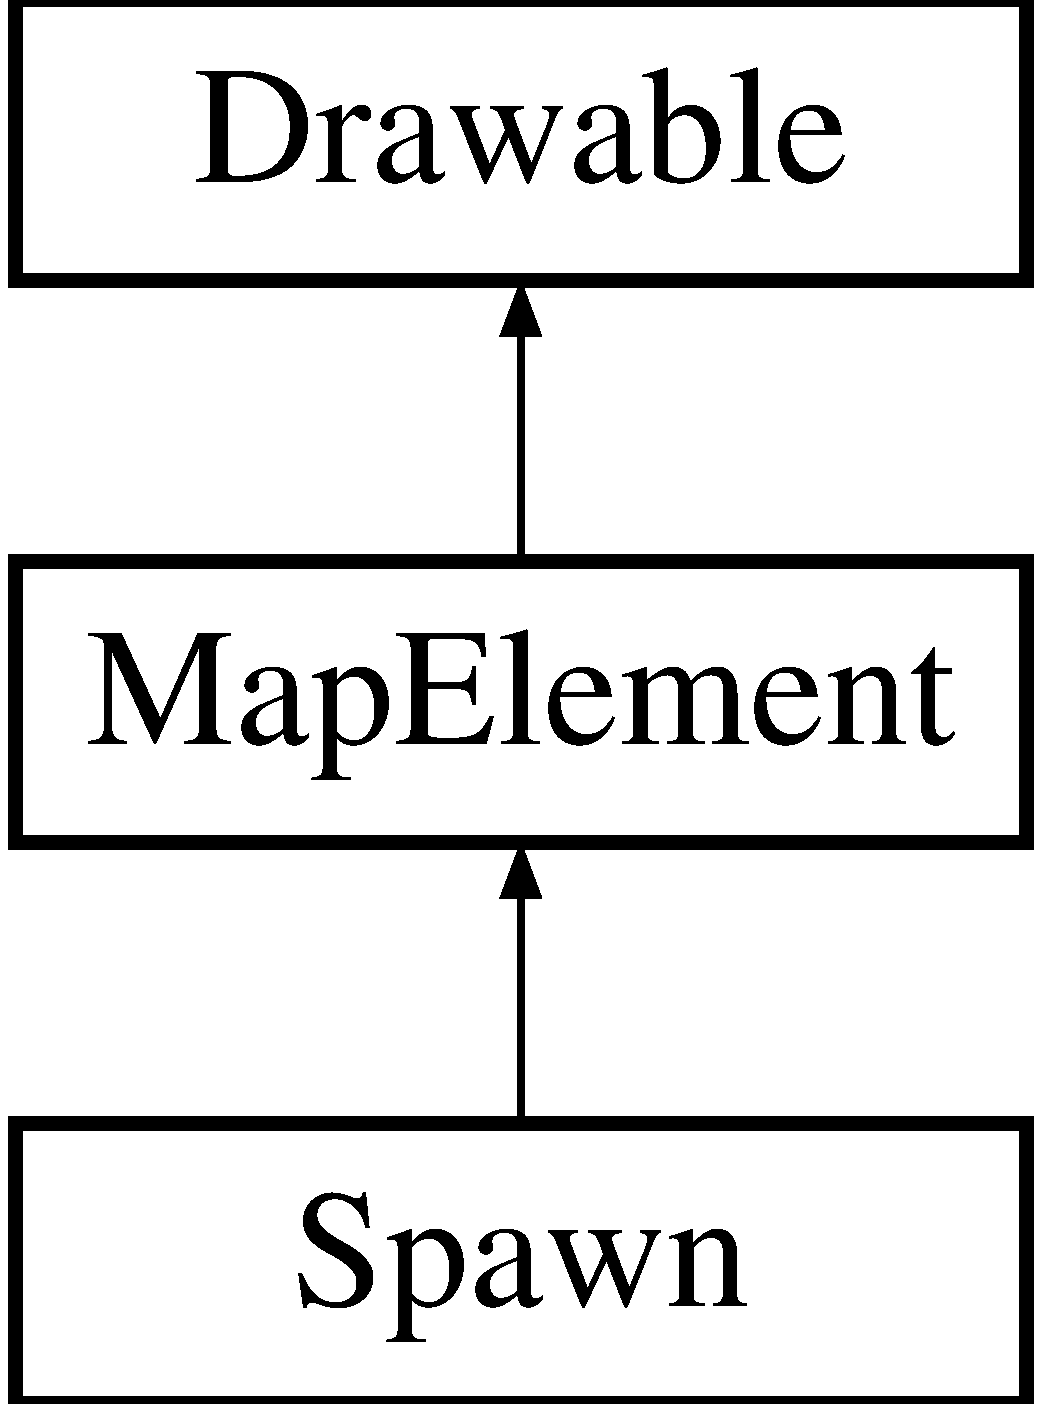
\includegraphics[height=3.000000cm]{class_spawn}
\end{center}
\end{figure}
\subsection*{Metody publiczne}
\begin{DoxyCompactItemize}
\item 
\hyperlink{class_spawn_a972290baedf94f776541be6039ee7d75}{Spawn} (int, \hyperlink{struct_position}{Position}, \hyperlink{struct_position}{Position})
\begin{DoxyCompactList}\small\item\em Konstruktor. \end{DoxyCompactList}\item 
\hyperlink{class_spawn_a54ab1e49c79ee947204f920046164829}{Spawn} (int, double, double, \hyperlink{struct_position}{Position})
\begin{DoxyCompactList}\small\item\em Konstruktor. \end{DoxyCompactList}\item 
void \hyperlink{class_spawn_afce802a99344be2869d5723f930cb3f4}{add\-Vehicle} (\hyperlink{_types_8h_a564207d327881e8bcfa0843e1a874756}{P\-Vehicle})
\begin{DoxyCompactList}\small\item\em Dodawanie pojazdu do kolejki oczekujących na start. \end{DoxyCompactList}\item 
\hyperlink{_types_8h_a564207d327881e8bcfa0843e1a874756}{P\-Vehicle} \hyperlink{class_spawn_af9f3e004e311973f4c8983aa586869f4}{start\-Vehicle} ()
\begin{DoxyCompactList}\small\item\em Wyświetla pojazdy na mapie. \end{DoxyCompactList}\item 
bool \hyperlink{class_spawn_a343f21c11732fad395e1b9f5bf1a227e}{has\-Vehicles\-To\-Start} ()
\begin{DoxyCompactList}\small\item\em Zwraca informację, czy \hyperlink{class_spawn}{Spawn} posiada jeszcze elementy do wystartowania. \end{DoxyCompactList}\item 
virtual void \hyperlink{class_spawn_a725ac9cb33aff1b26b19ed3affecf692}{draw} (\hyperlink{class_scene}{Scene} $\ast$)
\begin{DoxyCompactList}\small\item\em Metoda odpowiadająca za rysowanie elementu. \end{DoxyCompactList}\item 
\hyperlink{_direction_8h_a224b9163917ac32fc95a60d8c1eec3aa}{Direction} \hyperlink{class_spawn_a4a8907eb45fc0a0168d75063b51456a1}{get\-Direction} () const 
\begin{DoxyCompactList}\small\item\em Pobieranie kierunku, w którym skierowany jest \hyperlink{class_spawn}{Spawn}. \end{DoxyCompactList}\item 
virtual \hyperlink{class_spawn_aea08036b23acdb06fd47eba35dc2a8cf}{$\sim$\-Spawn} ()
\end{DoxyCompactItemize}
\subsection*{Statyczne metody publiczne}
\begin{DoxyCompactItemize}
\item 
static bool \hyperlink{class_spawn_abe804575f38e55324e413283898b5d57}{is\-Not\-Spawn} (const \hyperlink{_types_8h_a4260a5280323637f8a1fa28e89b6ef14}{P\-Map\-Element} el)
\item 
static bool \hyperlink{class_spawn_a488b20e9deeebe095670804599a3ddc9}{spawn\-Has\-Vehicles\-To\-Start} (const \hyperlink{_types_8h_a4260a5280323637f8a1fa28e89b6ef14}{P\-Map\-Element} el)
\begin{DoxyCompactList}\small\item\em Metoda sprawdza czy dany \hyperlink{class_spawn}{Spawn} ma jeszcze pojazdy do wystartowania. \end{DoxyCompactList}\end{DoxyCompactItemize}
\subsection*{Metody prywatne}
\begin{DoxyCompactItemize}
\item 
void \hyperlink{class_spawn_aece1dda8039ac307dd9bfdf9c47fb1c0}{calculate\-Direction} (\hyperlink{struct_position}{Position})
\item 
\hyperlink{struct_position}{Position} \hyperlink{class_spawn_a9dd0bae055d82dba2d95c0fab52d14f7}{calculate\-Start\-Position} (int)
\end{DoxyCompactItemize}
\subsection*{Atrybuty prywatne}
\begin{DoxyCompactItemize}
\item 
vector$<$ \hyperlink{_types_8h_a564207d327881e8bcfa0843e1a874756}{P\-Vehicle} $>$ \hyperlink{class_spawn_a9796373f175f911096daa7ffda1186ea}{vehicles\-To\-Start}
\item 
\hyperlink{_direction_8h_a224b9163917ac32fc95a60d8c1eec3aa}{Direction} \hyperlink{class_spawn_a593c6fb8ae012980751c4364b8ebb5b5}{direction}
\end{DoxyCompactItemize}
\subsection*{Dodatkowe Dziedziczone Składowe}


\subsection{Opis szczegółowy}
Klasa reprezentująca pojedynczy element służący jak punkt początkowy i końcowy dla pojazdów i pieszych. 

\subsection{Dokumentacja konstruktora i destruktora}
\hypertarget{class_spawn_a972290baedf94f776541be6039ee7d75}{\index{Spawn@{Spawn}!Spawn@{Spawn}}
\index{Spawn@{Spawn}!Spawn@{Spawn}}
\subsubsection[{Spawn}]{\setlength{\rightskip}{0pt plus 5cm}Spawn\-::\-Spawn (
\begin{DoxyParamCaption}
\item[{int}]{id\-\_\-, }
\item[{{\bf Position}}]{position\-\_\-, }
\item[{{\bf Position}}]{neighbor\-Pos\-\_\-}
\end{DoxyParamCaption}
)}}\label{class_spawn_a972290baedf94f776541be6039ee7d75}


Konstruktor. 

\hypertarget{class_spawn_a54ab1e49c79ee947204f920046164829}{\index{Spawn@{Spawn}!Spawn@{Spawn}}
\index{Spawn@{Spawn}!Spawn@{Spawn}}
\subsubsection[{Spawn}]{\setlength{\rightskip}{0pt plus 5cm}Spawn\-::\-Spawn (
\begin{DoxyParamCaption}
\item[{int}]{id\-\_\-, }
\item[{double}]{x\-\_\-, }
\item[{double}]{y\-\_\-, }
\item[{{\bf Position}}]{neighbor\-Pos\-\_\-}
\end{DoxyParamCaption}
)}}\label{class_spawn_a54ab1e49c79ee947204f920046164829}


Konstruktor. 

\hypertarget{class_spawn_aea08036b23acdb06fd47eba35dc2a8cf}{\index{Spawn@{Spawn}!$\sim$\-Spawn@{$\sim$\-Spawn}}
\index{$\sim$\-Spawn@{$\sim$\-Spawn}!Spawn@{Spawn}}
\subsubsection[{$\sim$\-Spawn}]{\setlength{\rightskip}{0pt plus 5cm}Spawn\-::$\sim$\-Spawn (
\begin{DoxyParamCaption}
{}
\end{DoxyParamCaption}
)\hspace{0.3cm}{\ttfamily [virtual]}}}\label{class_spawn_aea08036b23acdb06fd47eba35dc2a8cf}


\subsection{Dokumentacja funkcji składowych}
\hypertarget{class_spawn_afce802a99344be2869d5723f930cb3f4}{\index{Spawn@{Spawn}!add\-Vehicle@{add\-Vehicle}}
\index{add\-Vehicle@{add\-Vehicle}!Spawn@{Spawn}}
\subsubsection[{add\-Vehicle}]{\setlength{\rightskip}{0pt plus 5cm}void Spawn\-::add\-Vehicle (
\begin{DoxyParamCaption}
\item[{{\bf P\-Vehicle}}]{v\-\_\-}
\end{DoxyParamCaption}
)}}\label{class_spawn_afce802a99344be2869d5723f930cb3f4}


Dodawanie pojazdu do kolejki oczekujących na start. 

\hypertarget{class_spawn_aece1dda8039ac307dd9bfdf9c47fb1c0}{\index{Spawn@{Spawn}!calculate\-Direction@{calculate\-Direction}}
\index{calculate\-Direction@{calculate\-Direction}!Spawn@{Spawn}}
\subsubsection[{calculate\-Direction}]{\setlength{\rightskip}{0pt plus 5cm}void Spawn\-::calculate\-Direction (
\begin{DoxyParamCaption}
\item[{{\bf Position}}]{neighbor\-Pos\-\_\-}
\end{DoxyParamCaption}
)\hspace{0.3cm}{\ttfamily [private]}}}\label{class_spawn_aece1dda8039ac307dd9bfdf9c47fb1c0}
\hypertarget{class_spawn_a9dd0bae055d82dba2d95c0fab52d14f7}{\index{Spawn@{Spawn}!calculate\-Start\-Position@{calculate\-Start\-Position}}
\index{calculate\-Start\-Position@{calculate\-Start\-Position}!Spawn@{Spawn}}
\subsubsection[{calculate\-Start\-Position}]{\setlength{\rightskip}{0pt plus 5cm}{\bf Position} Spawn\-::calculate\-Start\-Position (
\begin{DoxyParamCaption}
\item[{int}]{lane\-\_\-}
\end{DoxyParamCaption}
)\hspace{0.3cm}{\ttfamily [private]}}}\label{class_spawn_a9dd0bae055d82dba2d95c0fab52d14f7}
\hypertarget{class_spawn_a725ac9cb33aff1b26b19ed3affecf692}{\index{Spawn@{Spawn}!draw@{draw}}
\index{draw@{draw}!Spawn@{Spawn}}
\subsubsection[{draw}]{\setlength{\rightskip}{0pt plus 5cm}void Spawn\-::draw (
\begin{DoxyParamCaption}
\item[{{\bf Scene} $\ast$}]{scene}
\end{DoxyParamCaption}
)\hspace{0.3cm}{\ttfamily [virtual]}}}\label{class_spawn_a725ac9cb33aff1b26b19ed3affecf692}


Metoda odpowiadająca za rysowanie elementu. 



Implementuje \hyperlink{class_map_element_aa76ca7443c4f6a6683f68f44909b90d3}{Map\-Element}.

\hypertarget{class_spawn_a4a8907eb45fc0a0168d75063b51456a1}{\index{Spawn@{Spawn}!get\-Direction@{get\-Direction}}
\index{get\-Direction@{get\-Direction}!Spawn@{Spawn}}
\subsubsection[{get\-Direction}]{\setlength{\rightskip}{0pt plus 5cm}{\bf Direction} Spawn\-::get\-Direction (
\begin{DoxyParamCaption}
{}
\end{DoxyParamCaption}
) const\hspace{0.3cm}{\ttfamily [inline]}}}\label{class_spawn_a4a8907eb45fc0a0168d75063b51456a1}


Pobieranie kierunku, w którym skierowany jest \hyperlink{class_spawn}{Spawn}. 

\hypertarget{class_spawn_a343f21c11732fad395e1b9f5bf1a227e}{\index{Spawn@{Spawn}!has\-Vehicles\-To\-Start@{has\-Vehicles\-To\-Start}}
\index{has\-Vehicles\-To\-Start@{has\-Vehicles\-To\-Start}!Spawn@{Spawn}}
\subsubsection[{has\-Vehicles\-To\-Start}]{\setlength{\rightskip}{0pt plus 5cm}bool Spawn\-::has\-Vehicles\-To\-Start (
\begin{DoxyParamCaption}
{}
\end{DoxyParamCaption}
)}}\label{class_spawn_a343f21c11732fad395e1b9f5bf1a227e}


Zwraca informację, czy \hyperlink{class_spawn}{Spawn} posiada jeszcze elementy do wystartowania. 

\hypertarget{class_spawn_abe804575f38e55324e413283898b5d57}{\index{Spawn@{Spawn}!is\-Not\-Spawn@{is\-Not\-Spawn}}
\index{is\-Not\-Spawn@{is\-Not\-Spawn}!Spawn@{Spawn}}
\subsubsection[{is\-Not\-Spawn}]{\setlength{\rightskip}{0pt plus 5cm}static bool Spawn\-::is\-Not\-Spawn (
\begin{DoxyParamCaption}
\item[{const {\bf P\-Map\-Element}}]{el}
\end{DoxyParamCaption}
)\hspace{0.3cm}{\ttfamily [inline]}, {\ttfamily [static]}}}\label{class_spawn_abe804575f38e55324e413283898b5d57}
\hypertarget{class_spawn_a488b20e9deeebe095670804599a3ddc9}{\index{Spawn@{Spawn}!spawn\-Has\-Vehicles\-To\-Start@{spawn\-Has\-Vehicles\-To\-Start}}
\index{spawn\-Has\-Vehicles\-To\-Start@{spawn\-Has\-Vehicles\-To\-Start}!Spawn@{Spawn}}
\subsubsection[{spawn\-Has\-Vehicles\-To\-Start}]{\setlength{\rightskip}{0pt plus 5cm}static bool Spawn\-::spawn\-Has\-Vehicles\-To\-Start (
\begin{DoxyParamCaption}
\item[{const {\bf P\-Map\-Element}}]{el}
\end{DoxyParamCaption}
)\hspace{0.3cm}{\ttfamily [inline]}, {\ttfamily [static]}}}\label{class_spawn_a488b20e9deeebe095670804599a3ddc9}


Metoda sprawdza czy dany \hyperlink{class_spawn}{Spawn} ma jeszcze pojazdy do wystartowania. 

\hypertarget{class_spawn_af9f3e004e311973f4c8983aa586869f4}{\index{Spawn@{Spawn}!start\-Vehicle@{start\-Vehicle}}
\index{start\-Vehicle@{start\-Vehicle}!Spawn@{Spawn}}
\subsubsection[{start\-Vehicle}]{\setlength{\rightskip}{0pt plus 5cm}{\bf P\-Vehicle} Spawn\-::start\-Vehicle (
\begin{DoxyParamCaption}
{}
\end{DoxyParamCaption}
)}}\label{class_spawn_af9f3e004e311973f4c8983aa586869f4}


Wyświetla pojazdy na mapie. 



\subsection{Dokumentacja atrybutów składowych}
\hypertarget{class_spawn_a593c6fb8ae012980751c4364b8ebb5b5}{\index{Spawn@{Spawn}!direction@{direction}}
\index{direction@{direction}!Spawn@{Spawn}}
\subsubsection[{direction}]{\setlength{\rightskip}{0pt plus 5cm}{\bf Direction} Spawn\-::direction\hspace{0.3cm}{\ttfamily [private]}}}\label{class_spawn_a593c6fb8ae012980751c4364b8ebb5b5}
\hypertarget{class_spawn_a9796373f175f911096daa7ffda1186ea}{\index{Spawn@{Spawn}!vehicles\-To\-Start@{vehicles\-To\-Start}}
\index{vehicles\-To\-Start@{vehicles\-To\-Start}!Spawn@{Spawn}}
\subsubsection[{vehicles\-To\-Start}]{\setlength{\rightskip}{0pt plus 5cm}vector$<${\bf P\-Vehicle}$>$ Spawn\-::vehicles\-To\-Start\hspace{0.3cm}{\ttfamily [private]}}}\label{class_spawn_a9796373f175f911096daa7ffda1186ea}


Dokumentacja dla tej klasy została wygenerowana z plików\-:\begin{DoxyCompactItemize}
\item 
src/\hyperlink{_spawn_8h}{Spawn.\-h}\item 
src/\hyperlink{_spawn_8cpp}{Spawn.\-cpp}\end{DoxyCompactItemize}

\hypertarget{class_spawning_pedestrians_runnable}{\section{Dokumentacja klasy Spawning\-Pedestrians\-Runnable}
\label{class_spawning_pedestrians_runnable}\index{Spawning\-Pedestrians\-Runnable@{Spawning\-Pedestrians\-Runnable}}
}


Klasa obsługująca powstawanie pieszych na planszy.  




{\ttfamily \#include $<$Spawning\-Pedestrians\-Runnable.\-h$>$}

\subsection*{Metody publiczne}
\begin{DoxyCompactItemize}
\item 
\hyperlink{class_spawning_pedestrians_runnable_a9d38055720541b747af740af852461bf}{Spawning\-Pedestrians\-Runnable} (\hyperlink{class_scene}{Scene} $\ast$, \hyperlink{class_simulator}{Simulator} $\ast$)
\begin{DoxyCompactList}\small\item\em Konstruktor. \end{DoxyCompactList}\item 
void \hyperlink{class_spawning_pedestrians_runnable_acba967ae5ead3b5ceab0e620417f98c4}{run} ()
\item 
void \hyperlink{class_spawning_pedestrians_runnable_aeac5a206439673b58551a247ab2c270d}{stop\-Thread} ()
\begin{DoxyCompactList}\small\item\em Metoda służąca do zatrzymywania działania wątku. \end{DoxyCompactList}\end{DoxyCompactItemize}
\subsection*{Atrybuty prywatne}
\begin{DoxyCompactItemize}
\item 
\hyperlink{class_scene}{Scene} $\ast$ \hyperlink{class_spawning_pedestrians_runnable_af9ce8e24f1f5f6ce1800192f75592023}{scene}
\item 
\hyperlink{class_simulator}{Simulator} $\ast$ \hyperlink{class_spawning_pedestrians_runnable_a5eeaca249d8d0b3ec9d263f172eee0dc}{simulator}
\item 
volatile bool \hyperlink{class_spawning_pedestrians_runnable_ad58c1c726a1f411f958d09ddab29325b}{go}
\end{DoxyCompactItemize}


\subsection{Opis szczegółowy}
Klasa obsługująca powstawanie pieszych na planszy. 

\subsection{Dokumentacja konstruktora i destruktora}
\hypertarget{class_spawning_pedestrians_runnable_a9d38055720541b747af740af852461bf}{\index{Spawning\-Pedestrians\-Runnable@{Spawning\-Pedestrians\-Runnable}!Spawning\-Pedestrians\-Runnable@{Spawning\-Pedestrians\-Runnable}}
\index{Spawning\-Pedestrians\-Runnable@{Spawning\-Pedestrians\-Runnable}!SpawningPedestriansRunnable@{Spawning\-Pedestrians\-Runnable}}
\subsubsection[{Spawning\-Pedestrians\-Runnable}]{\setlength{\rightskip}{0pt plus 5cm}Spawning\-Pedestrians\-Runnable\-::\-Spawning\-Pedestrians\-Runnable (
\begin{DoxyParamCaption}
\item[{{\bf Scene} $\ast$}]{scene\-\_\-, }
\item[{{\bf Simulator} $\ast$}]{simulator\-\_\-}
\end{DoxyParamCaption}
)}}\label{class_spawning_pedestrians_runnable_a9d38055720541b747af740af852461bf}


Konstruktor. 



\subsection{Dokumentacja funkcji składowych}
\hypertarget{class_spawning_pedestrians_runnable_acba967ae5ead3b5ceab0e620417f98c4}{\index{Spawning\-Pedestrians\-Runnable@{Spawning\-Pedestrians\-Runnable}!run@{run}}
\index{run@{run}!SpawningPedestriansRunnable@{Spawning\-Pedestrians\-Runnable}}
\subsubsection[{run}]{\setlength{\rightskip}{0pt plus 5cm}void Spawning\-Pedestrians\-Runnable\-::run (
\begin{DoxyParamCaption}
{}
\end{DoxyParamCaption}
)}}\label{class_spawning_pedestrians_runnable_acba967ae5ead3b5ceab0e620417f98c4}
To jest metoda przeciążona, udostępniona dla wygody. Różni się od powyższej metody tylko zestawem akceptowanych argumentów. \hypertarget{class_spawning_pedestrians_runnable_aeac5a206439673b58551a247ab2c270d}{\index{Spawning\-Pedestrians\-Runnable@{Spawning\-Pedestrians\-Runnable}!stop\-Thread@{stop\-Thread}}
\index{stop\-Thread@{stop\-Thread}!SpawningPedestriansRunnable@{Spawning\-Pedestrians\-Runnable}}
\subsubsection[{stop\-Thread}]{\setlength{\rightskip}{0pt plus 5cm}void Spawning\-Pedestrians\-Runnable\-::stop\-Thread (
\begin{DoxyParamCaption}
{}
\end{DoxyParamCaption}
)}}\label{class_spawning_pedestrians_runnable_aeac5a206439673b58551a247ab2c270d}


Metoda służąca do zatrzymywania działania wątku. 



\subsection{Dokumentacja atrybutów składowych}
\hypertarget{class_spawning_pedestrians_runnable_ad58c1c726a1f411f958d09ddab29325b}{\index{Spawning\-Pedestrians\-Runnable@{Spawning\-Pedestrians\-Runnable}!go@{go}}
\index{go@{go}!SpawningPedestriansRunnable@{Spawning\-Pedestrians\-Runnable}}
\subsubsection[{go}]{\setlength{\rightskip}{0pt plus 5cm}volatile bool Spawning\-Pedestrians\-Runnable\-::go\hspace{0.3cm}{\ttfamily [private]}}}\label{class_spawning_pedestrians_runnable_ad58c1c726a1f411f958d09ddab29325b}
\hypertarget{class_spawning_pedestrians_runnable_af9ce8e24f1f5f6ce1800192f75592023}{\index{Spawning\-Pedestrians\-Runnable@{Spawning\-Pedestrians\-Runnable}!scene@{scene}}
\index{scene@{scene}!SpawningPedestriansRunnable@{Spawning\-Pedestrians\-Runnable}}
\subsubsection[{scene}]{\setlength{\rightskip}{0pt plus 5cm}{\bf Scene}$\ast$ Spawning\-Pedestrians\-Runnable\-::scene\hspace{0.3cm}{\ttfamily [private]}}}\label{class_spawning_pedestrians_runnable_af9ce8e24f1f5f6ce1800192f75592023}
\hypertarget{class_spawning_pedestrians_runnable_a5eeaca249d8d0b3ec9d263f172eee0dc}{\index{Spawning\-Pedestrians\-Runnable@{Spawning\-Pedestrians\-Runnable}!simulator@{simulator}}
\index{simulator@{simulator}!SpawningPedestriansRunnable@{Spawning\-Pedestrians\-Runnable}}
\subsubsection[{simulator}]{\setlength{\rightskip}{0pt plus 5cm}{\bf Simulator}$\ast$ Spawning\-Pedestrians\-Runnable\-::simulator\hspace{0.3cm}{\ttfamily [private]}}}\label{class_spawning_pedestrians_runnable_a5eeaca249d8d0b3ec9d263f172eee0dc}


Dokumentacja dla tej klasy została wygenerowana z plików\-:\begin{DoxyCompactItemize}
\item 
src/\hyperlink{_spawning_pedestrians_runnable_8h}{Spawning\-Pedestrians\-Runnable.\-h}\item 
src/\hyperlink{_spawning_pedestrians_runnable_8cpp}{Spawning\-Pedestrians\-Runnable.\-cpp}\end{DoxyCompactItemize}

\hypertarget{class_spawning_vehicles_runnable}{\section{Dokumentacja klasy Spawning\-Vehicles\-Runnable}
\label{class_spawning_vehicles_runnable}\index{Spawning\-Vehicles\-Runnable@{Spawning\-Vehicles\-Runnable}}
}


Klasa obsługujaca powstawanie pojazdów na planszy w odpowiednich punktach \hyperlink{class_spawn}{Spawn}.  




{\ttfamily \#include $<$Spawning\-Vehicles\-Runnable.\-h$>$}

\subsection*{Metody publiczne}
\begin{DoxyCompactItemize}
\item 
\hyperlink{class_spawning_vehicles_runnable_a368400e286ab2536c4fd5a27251d8d2d}{Spawning\-Vehicles\-Runnable} (std\-::vector$<$ \hyperlink{_types_8h_a4260a5280323637f8a1fa28e89b6ef14}{P\-Map\-Element} $>$, \hyperlink{class_simulator}{Simulator} $\ast$)
\begin{DoxyCompactList}\small\item\em Konstruktor. \end{DoxyCompactList}\item 
void \hyperlink{class_spawning_vehicles_runnable_a3987c607c9c315ec9e66552d1cb0f799}{run} ()
\item 
void \hyperlink{class_spawning_vehicles_runnable_aa50e5fafaf1050a72658b0364c0bf88a}{stop\-Thread} ()
\begin{DoxyCompactList}\small\item\em Metoda służąca do zatrzymywania wątku. \end{DoxyCompactList}\end{DoxyCompactItemize}
\subsection*{Atrybuty prywatne}
\begin{DoxyCompactItemize}
\item 
std\-::vector$<$ \hyperlink{_types_8h_a4260a5280323637f8a1fa28e89b6ef14}{P\-Map\-Element} $>$ \hyperlink{class_spawning_vehicles_runnable_a1a9c575abd9e800d8b95a429b70be951}{spawns}
\item 
\hyperlink{class_simulator}{Simulator} $\ast$ \hyperlink{class_spawning_vehicles_runnable_a42bd4b9c441492b4206941856e140e3f}{simulator}
\item 
volatile bool \hyperlink{class_spawning_vehicles_runnable_ab868348a67a2995fc163b2155bfccb66}{go}
\end{DoxyCompactItemize}


\subsection{Opis szczegółowy}
Klasa obsługujaca powstawanie pojazdów na planszy w odpowiednich punktach \hyperlink{class_spawn}{Spawn}. 

\subsection{Dokumentacja konstruktora i destruktora}
\hypertarget{class_spawning_vehicles_runnable_a368400e286ab2536c4fd5a27251d8d2d}{\index{Spawning\-Vehicles\-Runnable@{Spawning\-Vehicles\-Runnable}!Spawning\-Vehicles\-Runnable@{Spawning\-Vehicles\-Runnable}}
\index{Spawning\-Vehicles\-Runnable@{Spawning\-Vehicles\-Runnable}!SpawningVehiclesRunnable@{Spawning\-Vehicles\-Runnable}}
\subsubsection[{Spawning\-Vehicles\-Runnable}]{\setlength{\rightskip}{0pt plus 5cm}Spawning\-Vehicles\-Runnable\-::\-Spawning\-Vehicles\-Runnable (
\begin{DoxyParamCaption}
\item[{std\-::vector$<$ {\bf P\-Map\-Element} $>$}]{spawns\-\_\-, }
\item[{{\bf Simulator} $\ast$}]{simulator\-\_\-}
\end{DoxyParamCaption}
)}}\label{class_spawning_vehicles_runnable_a368400e286ab2536c4fd5a27251d8d2d}


Konstruktor. 



\subsection{Dokumentacja funkcji składowych}
\hypertarget{class_spawning_vehicles_runnable_a3987c607c9c315ec9e66552d1cb0f799}{\index{Spawning\-Vehicles\-Runnable@{Spawning\-Vehicles\-Runnable}!run@{run}}
\index{run@{run}!SpawningVehiclesRunnable@{Spawning\-Vehicles\-Runnable}}
\subsubsection[{run}]{\setlength{\rightskip}{0pt plus 5cm}void Spawning\-Vehicles\-Runnable\-::run (
\begin{DoxyParamCaption}
{}
\end{DoxyParamCaption}
)}}\label{class_spawning_vehicles_runnable_a3987c607c9c315ec9e66552d1cb0f799}
To jest metoda przeciążona, udostępniona dla wygody. Różni się od powyższej metody tylko zestawem akceptowanych argumentów. \hypertarget{class_spawning_vehicles_runnable_aa50e5fafaf1050a72658b0364c0bf88a}{\index{Spawning\-Vehicles\-Runnable@{Spawning\-Vehicles\-Runnable}!stop\-Thread@{stop\-Thread}}
\index{stop\-Thread@{stop\-Thread}!SpawningVehiclesRunnable@{Spawning\-Vehicles\-Runnable}}
\subsubsection[{stop\-Thread}]{\setlength{\rightskip}{0pt plus 5cm}void Spawning\-Vehicles\-Runnable\-::stop\-Thread (
\begin{DoxyParamCaption}
{}
\end{DoxyParamCaption}
)}}\label{class_spawning_vehicles_runnable_aa50e5fafaf1050a72658b0364c0bf88a}


Metoda służąca do zatrzymywania wątku. 



\subsection{Dokumentacja atrybutów składowych}
\hypertarget{class_spawning_vehicles_runnable_ab868348a67a2995fc163b2155bfccb66}{\index{Spawning\-Vehicles\-Runnable@{Spawning\-Vehicles\-Runnable}!go@{go}}
\index{go@{go}!SpawningVehiclesRunnable@{Spawning\-Vehicles\-Runnable}}
\subsubsection[{go}]{\setlength{\rightskip}{0pt plus 5cm}volatile bool Spawning\-Vehicles\-Runnable\-::go\hspace{0.3cm}{\ttfamily [private]}}}\label{class_spawning_vehicles_runnable_ab868348a67a2995fc163b2155bfccb66}
\hypertarget{class_spawning_vehicles_runnable_a42bd4b9c441492b4206941856e140e3f}{\index{Spawning\-Vehicles\-Runnable@{Spawning\-Vehicles\-Runnable}!simulator@{simulator}}
\index{simulator@{simulator}!SpawningVehiclesRunnable@{Spawning\-Vehicles\-Runnable}}
\subsubsection[{simulator}]{\setlength{\rightskip}{0pt plus 5cm}{\bf Simulator}$\ast$ Spawning\-Vehicles\-Runnable\-::simulator\hspace{0.3cm}{\ttfamily [private]}}}\label{class_spawning_vehicles_runnable_a42bd4b9c441492b4206941856e140e3f}
\hypertarget{class_spawning_vehicles_runnable_a1a9c575abd9e800d8b95a429b70be951}{\index{Spawning\-Vehicles\-Runnable@{Spawning\-Vehicles\-Runnable}!spawns@{spawns}}
\index{spawns@{spawns}!SpawningVehiclesRunnable@{Spawning\-Vehicles\-Runnable}}
\subsubsection[{spawns}]{\setlength{\rightskip}{0pt plus 5cm}std\-::vector$<${\bf P\-Map\-Element}$>$ Spawning\-Vehicles\-Runnable\-::spawns\hspace{0.3cm}{\ttfamily [private]}}}\label{class_spawning_vehicles_runnable_a1a9c575abd9e800d8b95a429b70be951}


Dokumentacja dla tej klasy została wygenerowana z plików\-:\begin{DoxyCompactItemize}
\item 
src/\hyperlink{_spawning_vehicles_runnable_8h}{Spawning\-Vehicles\-Runnable.\-h}\item 
src/\hyperlink{_spawning_vehicles_runnable_8cpp}{Spawning\-Vehicles\-Runnable.\-cpp}\end{DoxyCompactItemize}

\hypertarget{class_vehicle}{\section{Dokumentacja klasy Vehicle}
\label{class_vehicle}\index{Vehicle@{Vehicle}}
}


Klasa odpowiadająca za pojazdy, ich poruszanie się po planszy, komunikację ze skrzyżowaniami, Spawnami, trasę przejazdu.  




{\ttfamily \#include $<$Vehicle.\-h$>$}

Diagram dziedziczenia dla Vehicle\begin{figure}[H]
\begin{center}
\leavevmode
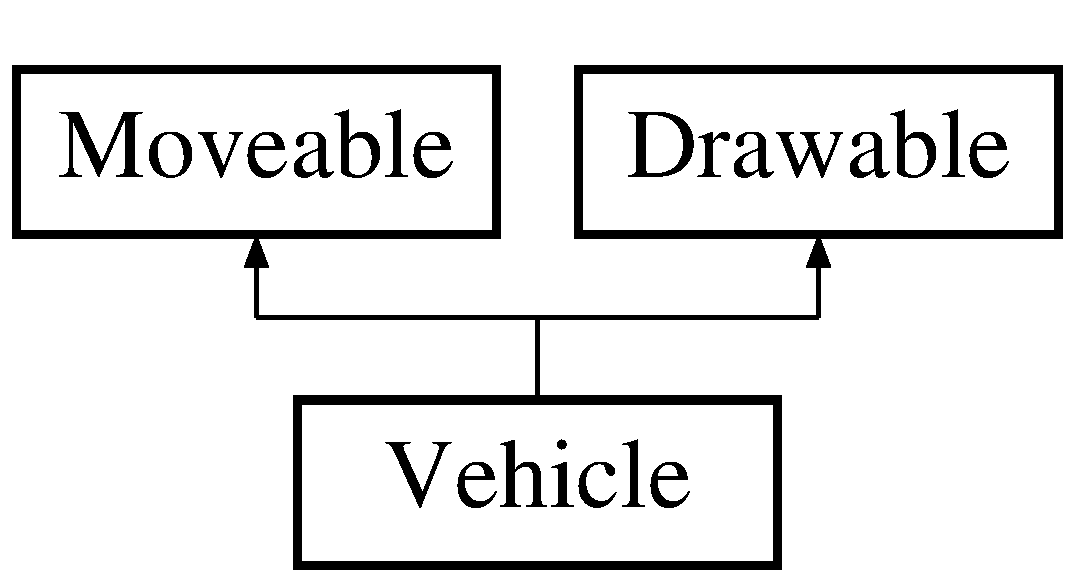
\includegraphics[height=2.000000cm]{class_vehicle}
\end{center}
\end{figure}
\subsection*{Metody publiczne}
\begin{DoxyCompactItemize}
\item 
\hyperlink{class_vehicle_acf02f2a9fb11d57389e3cc9f799293f7}{Vehicle} (int, string, int, string, float, float, float, int destination\-I\-D\-\_\-=-\/1)
\begin{DoxyCompactList}\small\item\em Konstruktor. \end{DoxyCompactList}\item 
virtual void \hyperlink{class_vehicle_a91c55b0a0ffc22c4f759452332b9ecd0}{draw} (\hyperlink{class_scene}{Scene} $\ast$)
\item 
virtual void \hyperlink{class_vehicle_ad5a55c6646313b8105b6dbb95b8eb89c}{calculate\-Position} ()
\begin{DoxyCompactList}\small\item\em Obliczanie kolejnej pozycji pojazdu. \end{DoxyCompactList}\item 
void \hyperlink{class_vehicle_a3e1a25a1506590ff2eaafdf6a7c85b65}{init} (\hyperlink{class_scene}{Scene} $\ast$)
\begin{DoxyCompactList}\small\item\em Inicjowanie pojazdu, ustawianie pozycji i kierunku początkowego. \end{DoxyCompactList}\item 
void \hyperlink{class_vehicle_a9ebd11c19fb0db693d4e3d6f5b45b5c2}{update\-Q\-Item\-On\-Scene} ()
\begin{DoxyCompactList}\small\item\em Odświeża obiekt q\-Item na scenie. \end{DoxyCompactList}\item 
void \hyperlink{class_vehicle_aa73d614ac4d0e4cf44aa0168cb89fb50}{check\-Collisions} (\hyperlink{class_scene}{Scene} $\ast$)
\begin{DoxyCompactList}\small\item\em Sprawdzanie kolizji i zapisywanie ich do wektora. \end{DoxyCompactList}\item 
bool \hyperlink{class_vehicle_aa0bcf3409ace641a42c87609a83e0ad8}{is\-Not\-Active} () const 
\begin{DoxyCompactList}\small\item\em Sprawdzanie czy obiekt jest aktywny, czy też powinniśmy go usunąć. \end{DoxyCompactList}\item 
double \hyperlink{class_vehicle_adf0dea6131864a4c28bb6bc79f78e44b}{get\-Length} () const 
\begin{DoxyCompactList}\small\item\em Pobieranie długości pojazdu. \end{DoxyCompactList}\item 
void \hyperlink{class_vehicle_ac880cb0a7eb1dac30267341e8034a86a}{set\-Lane} (int lane\-\_\-)
\begin{DoxyCompactList}\small\item\em Ustawianie pasa, po którym będzie się przemieszczał pojazd. \end{DoxyCompactList}\item 
void \hyperlink{class_vehicle_a90d48dc21a8c5d82149b35bed4caf84d}{set\-Path} (vector$<$ int $>$)
\begin{DoxyCompactList}\small\item\em Ustawianie drogi, po której pojazd będzie się poruszał. \end{DoxyCompactList}\item 
virtual \hyperlink{class_vehicle_a61ab140c755b8e0e824d54117cf4546f}{$\sim$\-Vehicle} ()
\end{DoxyCompactItemize}
\subsection*{Metody prywatne}
\begin{DoxyCompactItemize}
\item 
double \hyperlink{class_vehicle_aac21c89accf234d2c1c0229ff559dc25}{calculate\-Braking} () const 
\begin{DoxyCompactList}\small\item\em Oblicza drogę hamowania. \end{DoxyCompactList}\item 
void \hyperlink{class_vehicle_a518c4f4a17509fdb6e2031657894c346}{set\-Collision\-Item} ()
\begin{DoxyCompactList}\small\item\em Ustawia niewidoczny prostokąt służący do detekcji kolizji. \end{DoxyCompactList}\item 
void \hyperlink{class_vehicle_a8097bb51ec44c96d946a8cd1b963ab16}{check\-Collisions} ()
\begin{DoxyCompactList}\small\item\em Detekuje kolizje i zapewnia ich obsługę. \end{DoxyCompactList}\item 
void \hyperlink{class_vehicle_afb293273961ddcaa3367a9c4c1de4972}{check\-Collisions\-Vehicles} ()
\begin{DoxyCompactList}\small\item\em Detekuje kolizje z innymi pojazdami i zapewnia ich obsługę. \end{DoxyCompactList}\item 
void \hyperlink{class_vehicle_a3acdb31110e94042a96763100dccca2b}{calculate\-State} ()
\begin{DoxyCompactList}\small\item\em Ustawia kolejny stan pojazdu. \end{DoxyCompactList}\item 
bool \hyperlink{class_vehicle_a5944e3c99e136e780b488c8247c45554}{check\-Out\-Of\-Cross} ()
\begin{DoxyCompactList}\small\item\em Sprawdzanie czy pojazd jest już za skrzyżowaniem. \end{DoxyCompactList}\item 
bool \hyperlink{class_vehicle_a5702d5eba1fae66c11d744f1d7bfc71d}{check\-On\-Cross} ()
\begin{DoxyCompactList}\small\item\em Sprawdzanie czy pojazd wjechał na skrzyżowanie. \end{DoxyCompactList}\item 
bool \hyperlink{class_vehicle_af82b6feefaf07705011aca15835c940f}{check\-On\-Spawn} (\hyperlink{class_spawn}{Spawn} $\ast$s)
\begin{DoxyCompactList}\small\item\em Sprawdzanie czy pojazd przejechał przez \hyperlink{class_spawn}{Spawn}. \end{DoxyCompactList}\item 
void \hyperlink{class_vehicle_a3baf18e6b6b8f3c9a16a4d93ea16c46c}{position\-After\-Turn} ()
\begin{DoxyCompactList}\small\item\em Ustawianie odpowiedniej pozycji po wyjściu z zakrętu. \end{DoxyCompactList}\item 
void \hyperlink{class_vehicle_a85071a892f7e2b731e40d159897e21ec}{get\-Off\-Cross} ()
\begin{DoxyCompactList}\small\item\em Instrukcje wykonywane po wyjechaniu ze skrzyżowania. \end{DoxyCompactList}\item 
void \hyperlink{class_vehicle_af2e6c030a5be66b6fd669216fdb76b74}{move\-Forward} ()
\item 
void \hyperlink{class_vehicle_a862a647913e72fdfcbc5698486d4674d}{turn\-Left} ()
\item 
void \hyperlink{class_vehicle_a5a0f5be9d10f110b69d4f9680610403a}{turn\-Right} ()
\end{DoxyCompactItemize}
\subsection*{Atrybuty prywatne}
\begin{DoxyCompactItemize}
\item 
Q\-Graphics\-Rect\-Item $\ast$ \hyperlink{class_vehicle_a6de375e22bd723ba487c50489e569548}{q\-Item}
\item 
Q\-Graphics\-Rect\-Item $\ast$ \hyperlink{class_vehicle_a9bf00c3b511e214ab95d5da12e49633c}{q\-Collision\-Item}
\item 
double \hyperlink{class_vehicle_a675a8ef19fd15e2753bd963c19a4904c}{length}
\item 
int \hyperlink{class_vehicle_a7421a7a2d98b4ec6dfabd1041261aa03}{id}
\item 
int \hyperlink{class_vehicle_a4b941cb02036dc75ae4ad733e3493119}{start\-I\-D}
\item 
Q\-Color \hyperlink{class_vehicle_a290ebfd05412ee45125dbc282f724488}{color}
\item 
float \hyperlink{class_vehicle_a2742f50ec74d5b8ac0f81d3222842110}{reflex}
\item 
int \hyperlink{class_vehicle_a75d0148cd658133b6d6a550c27bfb936}{destination\-I\-D}
\item 
\hyperlink{_vehicle_state_8h_a75c52206c3c79acb62c0fddc66df3676}{Vehicle\-State} \hyperlink{class_vehicle_ab3541bd459598db80bb2748db1452feb}{state}
\item 
\hyperlink{class_cross}{Cross} $\ast$ \hyperlink{class_vehicle_a32fb5373b1808c23c25124ea2ce66b8c}{next\-Cross}
\item 
\hyperlink{class_cross}{Cross} $\ast$ \hyperlink{class_vehicle_af0dd745daa5f73c8e4b2f687effca686}{last\-Cross}
\item 
bool \hyperlink{class_vehicle_a7a5fe72aaf4d2f119a4dc58c4b35e36e}{on\-Cross}
\item 
vector$<$ int $>$ \hyperlink{class_vehicle_a8379932487731fc05e7c88bd0609c802}{path}
\item 
string \hyperlink{class_vehicle_a0aaf8072804d5034c24dc35772551b20}{driving\-Mode}
\item 
int \hyperlink{class_vehicle_a838acb6c559579924c5738e921886214}{lane}
\item 
double \hyperlink{class_vehicle_a4a1cd6d5bc788fa5e99ed463e6d104de}{dl}
\item 
vector$<$ \hyperlink{class_map_element}{Map\-Element} $\ast$ $>$ \hyperlink{class_vehicle_ade840ce20f05a39006a8a44a26ac42bf}{collides\-Map\-Elements}
\item 
bool \hyperlink{class_vehicle_a28f41cf00d7689c39e29bc951e3e0472}{collided\-Vehicles}
\item 
Q\-Point\-F \hyperlink{class_vehicle_ad04fb4832c299dd0508e3b335fa5ce20}{transform\-Origin\-Point\-To\-Set}
\item 
double \hyperlink{class_vehicle_a15bac66c5ee90f81529c9eb5ba2d7b3c}{rotation\-To\-Set}
\end{DoxyCompactItemize}
\subsection*{Dodatkowe Dziedziczone Składowe}


\subsection{Opis szczegółowy}
Klasa odpowiadająca za pojazdy, ich poruszanie się po planszy, komunikację ze skrzyżowaniami, Spawnami, trasę przejazdu. 

\subsection{Dokumentacja konstruktora i destruktora}
\hypertarget{class_vehicle_acf02f2a9fb11d57389e3cc9f799293f7}{\index{Vehicle@{Vehicle}!Vehicle@{Vehicle}}
\index{Vehicle@{Vehicle}!Vehicle@{Vehicle}}
\subsubsection[{Vehicle}]{\setlength{\rightskip}{0pt plus 5cm}Vehicle\-::\-Vehicle (
\begin{DoxyParamCaption}
\item[{int}]{id\-\_\-, }
\item[{string}]{type\-\_\-, }
\item[{int}]{start\-I\-D\-\_\-, }
\item[{string}]{color\-\_\-, }
\item[{float}]{max\-Speed\-\_\-, }
\item[{float}]{acceleration\-\_\-, }
\item[{float}]{reflex\-\_\-, }
\item[{int}]{destination\-I\-D\-\_\- = {\ttfamily -\/1}}
\end{DoxyParamCaption}
)}}\label{class_vehicle_acf02f2a9fb11d57389e3cc9f799293f7}


Konstruktor. 

\hypertarget{class_vehicle_a61ab140c755b8e0e824d54117cf4546f}{\index{Vehicle@{Vehicle}!$\sim$\-Vehicle@{$\sim$\-Vehicle}}
\index{$\sim$\-Vehicle@{$\sim$\-Vehicle}!Vehicle@{Vehicle}}
\subsubsection[{$\sim$\-Vehicle}]{\setlength{\rightskip}{0pt plus 5cm}Vehicle\-::$\sim$\-Vehicle (
\begin{DoxyParamCaption}
{}
\end{DoxyParamCaption}
)\hspace{0.3cm}{\ttfamily [virtual]}}}\label{class_vehicle_a61ab140c755b8e0e824d54117cf4546f}


\subsection{Dokumentacja funkcji składowych}
\hypertarget{class_vehicle_aac21c89accf234d2c1c0229ff559dc25}{\index{Vehicle@{Vehicle}!calculate\-Braking@{calculate\-Braking}}
\index{calculate\-Braking@{calculate\-Braking}!Vehicle@{Vehicle}}
\subsubsection[{calculate\-Braking}]{\setlength{\rightskip}{0pt plus 5cm}double Vehicle\-::calculate\-Braking (
\begin{DoxyParamCaption}
{}
\end{DoxyParamCaption}
) const\hspace{0.3cm}{\ttfamily [private]}}}\label{class_vehicle_aac21c89accf234d2c1c0229ff559dc25}


Oblicza drogę hamowania. 

\hypertarget{class_vehicle_ad5a55c6646313b8105b6dbb95b8eb89c}{\index{Vehicle@{Vehicle}!calculate\-Position@{calculate\-Position}}
\index{calculate\-Position@{calculate\-Position}!Vehicle@{Vehicle}}
\subsubsection[{calculate\-Position}]{\setlength{\rightskip}{0pt plus 5cm}void Vehicle\-::calculate\-Position (
\begin{DoxyParamCaption}
{}
\end{DoxyParamCaption}
)\hspace{0.3cm}{\ttfamily [virtual]}}}\label{class_vehicle_ad5a55c6646313b8105b6dbb95b8eb89c}


Obliczanie kolejnej pozycji pojazdu. 



Implementuje \hyperlink{class_moveable_a3e42cec7b55d6320553b1c40e2392cb9}{Moveable}.

\hypertarget{class_vehicle_a3acdb31110e94042a96763100dccca2b}{\index{Vehicle@{Vehicle}!calculate\-State@{calculate\-State}}
\index{calculate\-State@{calculate\-State}!Vehicle@{Vehicle}}
\subsubsection[{calculate\-State}]{\setlength{\rightskip}{0pt plus 5cm}void Vehicle\-::calculate\-State (
\begin{DoxyParamCaption}
{}
\end{DoxyParamCaption}
)\hspace{0.3cm}{\ttfamily [private]}}}\label{class_vehicle_a3acdb31110e94042a96763100dccca2b}


Ustawia kolejny stan pojazdu. 

\hypertarget{class_vehicle_a8097bb51ec44c96d946a8cd1b963ab16}{\index{Vehicle@{Vehicle}!check\-Collisions@{check\-Collisions}}
\index{check\-Collisions@{check\-Collisions}!Vehicle@{Vehicle}}
\subsubsection[{check\-Collisions}]{\setlength{\rightskip}{0pt plus 5cm}void Vehicle\-::check\-Collisions (
\begin{DoxyParamCaption}
{}
\end{DoxyParamCaption}
)\hspace{0.3cm}{\ttfamily [private]}}}\label{class_vehicle_a8097bb51ec44c96d946a8cd1b963ab16}


Detekuje kolizje i zapewnia ich obsługę. 

\hypertarget{class_vehicle_aa73d614ac4d0e4cf44aa0168cb89fb50}{\index{Vehicle@{Vehicle}!check\-Collisions@{check\-Collisions}}
\index{check\-Collisions@{check\-Collisions}!Vehicle@{Vehicle}}
\subsubsection[{check\-Collisions}]{\setlength{\rightskip}{0pt plus 5cm}void Vehicle\-::check\-Collisions (
\begin{DoxyParamCaption}
\item[{{\bf Scene} $\ast$}]{scene\-\_\-}
\end{DoxyParamCaption}
)}}\label{class_vehicle_aa73d614ac4d0e4cf44aa0168cb89fb50}


Sprawdzanie kolizji i zapisywanie ich do wektora. 

\hypertarget{class_vehicle_afb293273961ddcaa3367a9c4c1de4972}{\index{Vehicle@{Vehicle}!check\-Collisions\-Vehicles@{check\-Collisions\-Vehicles}}
\index{check\-Collisions\-Vehicles@{check\-Collisions\-Vehicles}!Vehicle@{Vehicle}}
\subsubsection[{check\-Collisions\-Vehicles}]{\setlength{\rightskip}{0pt plus 5cm}void Vehicle\-::check\-Collisions\-Vehicles (
\begin{DoxyParamCaption}
{}
\end{DoxyParamCaption}
)\hspace{0.3cm}{\ttfamily [private]}}}\label{class_vehicle_afb293273961ddcaa3367a9c4c1de4972}


Detekuje kolizje z innymi pojazdami i zapewnia ich obsługę. 

\hypertarget{class_vehicle_a5702d5eba1fae66c11d744f1d7bfc71d}{\index{Vehicle@{Vehicle}!check\-On\-Cross@{check\-On\-Cross}}
\index{check\-On\-Cross@{check\-On\-Cross}!Vehicle@{Vehicle}}
\subsubsection[{check\-On\-Cross}]{\setlength{\rightskip}{0pt plus 5cm}bool Vehicle\-::check\-On\-Cross (
\begin{DoxyParamCaption}
{}
\end{DoxyParamCaption}
)\hspace{0.3cm}{\ttfamily [private]}}}\label{class_vehicle_a5702d5eba1fae66c11d744f1d7bfc71d}


Sprawdzanie czy pojazd wjechał na skrzyżowanie. 

\hypertarget{class_vehicle_af82b6feefaf07705011aca15835c940f}{\index{Vehicle@{Vehicle}!check\-On\-Spawn@{check\-On\-Spawn}}
\index{check\-On\-Spawn@{check\-On\-Spawn}!Vehicle@{Vehicle}}
\subsubsection[{check\-On\-Spawn}]{\setlength{\rightskip}{0pt plus 5cm}bool Vehicle\-::check\-On\-Spawn (
\begin{DoxyParamCaption}
\item[{{\bf Spawn} $\ast$}]{s}
\end{DoxyParamCaption}
)\hspace{0.3cm}{\ttfamily [private]}}}\label{class_vehicle_af82b6feefaf07705011aca15835c940f}


Sprawdzanie czy pojazd przejechał przez \hyperlink{class_spawn}{Spawn}. 

\hypertarget{class_vehicle_a5944e3c99e136e780b488c8247c45554}{\index{Vehicle@{Vehicle}!check\-Out\-Of\-Cross@{check\-Out\-Of\-Cross}}
\index{check\-Out\-Of\-Cross@{check\-Out\-Of\-Cross}!Vehicle@{Vehicle}}
\subsubsection[{check\-Out\-Of\-Cross}]{\setlength{\rightskip}{0pt plus 5cm}bool Vehicle\-::check\-Out\-Of\-Cross (
\begin{DoxyParamCaption}
{}
\end{DoxyParamCaption}
)\hspace{0.3cm}{\ttfamily [private]}}}\label{class_vehicle_a5944e3c99e136e780b488c8247c45554}


Sprawdzanie czy pojazd jest już za skrzyżowaniem. 

\hypertarget{class_vehicle_a91c55b0a0ffc22c4f759452332b9ecd0}{\index{Vehicle@{Vehicle}!draw@{draw}}
\index{draw@{draw}!Vehicle@{Vehicle}}
\subsubsection[{draw}]{\setlength{\rightskip}{0pt plus 5cm}void Vehicle\-::draw (
\begin{DoxyParamCaption}
\item[{{\bf Scene} $\ast$}]{}
\end{DoxyParamCaption}
)\hspace{0.3cm}{\ttfamily [virtual]}}}\label{class_vehicle_a91c55b0a0ffc22c4f759452332b9ecd0}


Implementuje \hyperlink{class_drawable_a1e24b799e5b5f5494b25a42e2624692c}{Drawable}.

\hypertarget{class_vehicle_adf0dea6131864a4c28bb6bc79f78e44b}{\index{Vehicle@{Vehicle}!get\-Length@{get\-Length}}
\index{get\-Length@{get\-Length}!Vehicle@{Vehicle}}
\subsubsection[{get\-Length}]{\setlength{\rightskip}{0pt plus 5cm}double Vehicle\-::get\-Length (
\begin{DoxyParamCaption}
{}
\end{DoxyParamCaption}
) const\hspace{0.3cm}{\ttfamily [inline]}}}\label{class_vehicle_adf0dea6131864a4c28bb6bc79f78e44b}


Pobieranie długości pojazdu. 

\hypertarget{class_vehicle_a85071a892f7e2b731e40d159897e21ec}{\index{Vehicle@{Vehicle}!get\-Off\-Cross@{get\-Off\-Cross}}
\index{get\-Off\-Cross@{get\-Off\-Cross}!Vehicle@{Vehicle}}
\subsubsection[{get\-Off\-Cross}]{\setlength{\rightskip}{0pt plus 5cm}void Vehicle\-::get\-Off\-Cross (
\begin{DoxyParamCaption}
{}
\end{DoxyParamCaption}
)\hspace{0.3cm}{\ttfamily [private]}}}\label{class_vehicle_a85071a892f7e2b731e40d159897e21ec}


Instrukcje wykonywane po wyjechaniu ze skrzyżowania. 

\hypertarget{class_vehicle_a3e1a25a1506590ff2eaafdf6a7c85b65}{\index{Vehicle@{Vehicle}!init@{init}}
\index{init@{init}!Vehicle@{Vehicle}}
\subsubsection[{init}]{\setlength{\rightskip}{0pt plus 5cm}void Vehicle\-::init (
\begin{DoxyParamCaption}
\item[{{\bf Scene} $\ast$}]{scene\-\_\-}
\end{DoxyParamCaption}
)}}\label{class_vehicle_a3e1a25a1506590ff2eaafdf6a7c85b65}


Inicjowanie pojazdu, ustawianie pozycji i kierunku początkowego. 

\hypertarget{class_vehicle_aa0bcf3409ace641a42c87609a83e0ad8}{\index{Vehicle@{Vehicle}!is\-Not\-Active@{is\-Not\-Active}}
\index{is\-Not\-Active@{is\-Not\-Active}!Vehicle@{Vehicle}}
\subsubsection[{is\-Not\-Active}]{\setlength{\rightskip}{0pt plus 5cm}bool Vehicle\-::is\-Not\-Active (
\begin{DoxyParamCaption}
{}
\end{DoxyParamCaption}
) const\hspace{0.3cm}{\ttfamily [inline]}}}\label{class_vehicle_aa0bcf3409ace641a42c87609a83e0ad8}


Sprawdzanie czy obiekt jest aktywny, czy też powinniśmy go usunąć. 

\hypertarget{class_vehicle_af2e6c030a5be66b6fd669216fdb76b74}{\index{Vehicle@{Vehicle}!move\-Forward@{move\-Forward}}
\index{move\-Forward@{move\-Forward}!Vehicle@{Vehicle}}
\subsubsection[{move\-Forward}]{\setlength{\rightskip}{0pt plus 5cm}void Vehicle\-::move\-Forward (
\begin{DoxyParamCaption}
{}
\end{DoxyParamCaption}
)\hspace{0.3cm}{\ttfamily [private]}}}\label{class_vehicle_af2e6c030a5be66b6fd669216fdb76b74}
\hypertarget{class_vehicle_a3baf18e6b6b8f3c9a16a4d93ea16c46c}{\index{Vehicle@{Vehicle}!position\-After\-Turn@{position\-After\-Turn}}
\index{position\-After\-Turn@{position\-After\-Turn}!Vehicle@{Vehicle}}
\subsubsection[{position\-After\-Turn}]{\setlength{\rightskip}{0pt plus 5cm}void Vehicle\-::position\-After\-Turn (
\begin{DoxyParamCaption}
{}
\end{DoxyParamCaption}
)\hspace{0.3cm}{\ttfamily [private]}}}\label{class_vehicle_a3baf18e6b6b8f3c9a16a4d93ea16c46c}


Ustawianie odpowiedniej pozycji po wyjściu z zakrętu. 

\hypertarget{class_vehicle_a518c4f4a17509fdb6e2031657894c346}{\index{Vehicle@{Vehicle}!set\-Collision\-Item@{set\-Collision\-Item}}
\index{set\-Collision\-Item@{set\-Collision\-Item}!Vehicle@{Vehicle}}
\subsubsection[{set\-Collision\-Item}]{\setlength{\rightskip}{0pt plus 5cm}void Vehicle\-::set\-Collision\-Item (
\begin{DoxyParamCaption}
{}
\end{DoxyParamCaption}
)\hspace{0.3cm}{\ttfamily [private]}}}\label{class_vehicle_a518c4f4a17509fdb6e2031657894c346}


Ustawia niewidoczny prostokąt służący do detekcji kolizji. 

\hypertarget{class_vehicle_ac880cb0a7eb1dac30267341e8034a86a}{\index{Vehicle@{Vehicle}!set\-Lane@{set\-Lane}}
\index{set\-Lane@{set\-Lane}!Vehicle@{Vehicle}}
\subsubsection[{set\-Lane}]{\setlength{\rightskip}{0pt plus 5cm}void Vehicle\-::set\-Lane (
\begin{DoxyParamCaption}
\item[{int}]{lane\-\_\-}
\end{DoxyParamCaption}
)\hspace{0.3cm}{\ttfamily [inline]}}}\label{class_vehicle_ac880cb0a7eb1dac30267341e8034a86a}


Ustawianie pasa, po którym będzie się przemieszczał pojazd. 

\hypertarget{class_vehicle_a90d48dc21a8c5d82149b35bed4caf84d}{\index{Vehicle@{Vehicle}!set\-Path@{set\-Path}}
\index{set\-Path@{set\-Path}!Vehicle@{Vehicle}}
\subsubsection[{set\-Path}]{\setlength{\rightskip}{0pt plus 5cm}void Vehicle\-::set\-Path (
\begin{DoxyParamCaption}
\item[{vector$<$ int $>$}]{path\-\_\-}
\end{DoxyParamCaption}
)}}\label{class_vehicle_a90d48dc21a8c5d82149b35bed4caf84d}


Ustawianie drogi, po której pojazd będzie się poruszał. 

\hypertarget{class_vehicle_a862a647913e72fdfcbc5698486d4674d}{\index{Vehicle@{Vehicle}!turn\-Left@{turn\-Left}}
\index{turn\-Left@{turn\-Left}!Vehicle@{Vehicle}}
\subsubsection[{turn\-Left}]{\setlength{\rightskip}{0pt plus 5cm}void Vehicle\-::turn\-Left (
\begin{DoxyParamCaption}
{}
\end{DoxyParamCaption}
)\hspace{0.3cm}{\ttfamily [private]}}}\label{class_vehicle_a862a647913e72fdfcbc5698486d4674d}
\hypertarget{class_vehicle_a5a0f5be9d10f110b69d4f9680610403a}{\index{Vehicle@{Vehicle}!turn\-Right@{turn\-Right}}
\index{turn\-Right@{turn\-Right}!Vehicle@{Vehicle}}
\subsubsection[{turn\-Right}]{\setlength{\rightskip}{0pt plus 5cm}void Vehicle\-::turn\-Right (
\begin{DoxyParamCaption}
{}
\end{DoxyParamCaption}
)\hspace{0.3cm}{\ttfamily [private]}}}\label{class_vehicle_a5a0f5be9d10f110b69d4f9680610403a}
\hypertarget{class_vehicle_a9ebd11c19fb0db693d4e3d6f5b45b5c2}{\index{Vehicle@{Vehicle}!update\-Q\-Item\-On\-Scene@{update\-Q\-Item\-On\-Scene}}
\index{update\-Q\-Item\-On\-Scene@{update\-Q\-Item\-On\-Scene}!Vehicle@{Vehicle}}
\subsubsection[{update\-Q\-Item\-On\-Scene}]{\setlength{\rightskip}{0pt plus 5cm}void Vehicle\-::update\-Q\-Item\-On\-Scene (
\begin{DoxyParamCaption}
{}
\end{DoxyParamCaption}
)}}\label{class_vehicle_a9ebd11c19fb0db693d4e3d6f5b45b5c2}


Odświeża obiekt q\-Item na scenie. 



\subsection{Dokumentacja atrybutów składowych}
\hypertarget{class_vehicle_a28f41cf00d7689c39e29bc951e3e0472}{\index{Vehicle@{Vehicle}!collided\-Vehicles@{collided\-Vehicles}}
\index{collided\-Vehicles@{collided\-Vehicles}!Vehicle@{Vehicle}}
\subsubsection[{collided\-Vehicles}]{\setlength{\rightskip}{0pt plus 5cm}bool Vehicle\-::collided\-Vehicles\hspace{0.3cm}{\ttfamily [private]}}}\label{class_vehicle_a28f41cf00d7689c39e29bc951e3e0472}
\hypertarget{class_vehicle_ade840ce20f05a39006a8a44a26ac42bf}{\index{Vehicle@{Vehicle}!collides\-Map\-Elements@{collides\-Map\-Elements}}
\index{collides\-Map\-Elements@{collides\-Map\-Elements}!Vehicle@{Vehicle}}
\subsubsection[{collides\-Map\-Elements}]{\setlength{\rightskip}{0pt plus 5cm}vector$<${\bf Map\-Element}$\ast$$>$ Vehicle\-::collides\-Map\-Elements\hspace{0.3cm}{\ttfamily [private]}}}\label{class_vehicle_ade840ce20f05a39006a8a44a26ac42bf}
\hypertarget{class_vehicle_a290ebfd05412ee45125dbc282f724488}{\index{Vehicle@{Vehicle}!color@{color}}
\index{color@{color}!Vehicle@{Vehicle}}
\subsubsection[{color}]{\setlength{\rightskip}{0pt plus 5cm}Q\-Color Vehicle\-::color\hspace{0.3cm}{\ttfamily [private]}}}\label{class_vehicle_a290ebfd05412ee45125dbc282f724488}
\hypertarget{class_vehicle_a75d0148cd658133b6d6a550c27bfb936}{\index{Vehicle@{Vehicle}!destination\-I\-D@{destination\-I\-D}}
\index{destination\-I\-D@{destination\-I\-D}!Vehicle@{Vehicle}}
\subsubsection[{destination\-I\-D}]{\setlength{\rightskip}{0pt plus 5cm}int Vehicle\-::destination\-I\-D\hspace{0.3cm}{\ttfamily [private]}}}\label{class_vehicle_a75d0148cd658133b6d6a550c27bfb936}
\hypertarget{class_vehicle_a4a1cd6d5bc788fa5e99ed463e6d104de}{\index{Vehicle@{Vehicle}!dl@{dl}}
\index{dl@{dl}!Vehicle@{Vehicle}}
\subsubsection[{dl}]{\setlength{\rightskip}{0pt plus 5cm}double Vehicle\-::dl\hspace{0.3cm}{\ttfamily [private]}}}\label{class_vehicle_a4a1cd6d5bc788fa5e99ed463e6d104de}
\hypertarget{class_vehicle_a0aaf8072804d5034c24dc35772551b20}{\index{Vehicle@{Vehicle}!driving\-Mode@{driving\-Mode}}
\index{driving\-Mode@{driving\-Mode}!Vehicle@{Vehicle}}
\subsubsection[{driving\-Mode}]{\setlength{\rightskip}{0pt plus 5cm}string Vehicle\-::driving\-Mode\hspace{0.3cm}{\ttfamily [private]}}}\label{class_vehicle_a0aaf8072804d5034c24dc35772551b20}
\hypertarget{class_vehicle_a7421a7a2d98b4ec6dfabd1041261aa03}{\index{Vehicle@{Vehicle}!id@{id}}
\index{id@{id}!Vehicle@{Vehicle}}
\subsubsection[{id}]{\setlength{\rightskip}{0pt plus 5cm}int Vehicle\-::id\hspace{0.3cm}{\ttfamily [private]}}}\label{class_vehicle_a7421a7a2d98b4ec6dfabd1041261aa03}
\hypertarget{class_vehicle_a838acb6c559579924c5738e921886214}{\index{Vehicle@{Vehicle}!lane@{lane}}
\index{lane@{lane}!Vehicle@{Vehicle}}
\subsubsection[{lane}]{\setlength{\rightskip}{0pt plus 5cm}int Vehicle\-::lane\hspace{0.3cm}{\ttfamily [private]}}}\label{class_vehicle_a838acb6c559579924c5738e921886214}
\hypertarget{class_vehicle_af0dd745daa5f73c8e4b2f687effca686}{\index{Vehicle@{Vehicle}!last\-Cross@{last\-Cross}}
\index{last\-Cross@{last\-Cross}!Vehicle@{Vehicle}}
\subsubsection[{last\-Cross}]{\setlength{\rightskip}{0pt plus 5cm}{\bf Cross}$\ast$ Vehicle\-::last\-Cross\hspace{0.3cm}{\ttfamily [private]}}}\label{class_vehicle_af0dd745daa5f73c8e4b2f687effca686}
\hypertarget{class_vehicle_a675a8ef19fd15e2753bd963c19a4904c}{\index{Vehicle@{Vehicle}!length@{length}}
\index{length@{length}!Vehicle@{Vehicle}}
\subsubsection[{length}]{\setlength{\rightskip}{0pt plus 5cm}double Vehicle\-::length\hspace{0.3cm}{\ttfamily [private]}}}\label{class_vehicle_a675a8ef19fd15e2753bd963c19a4904c}
\hypertarget{class_vehicle_a32fb5373b1808c23c25124ea2ce66b8c}{\index{Vehicle@{Vehicle}!next\-Cross@{next\-Cross}}
\index{next\-Cross@{next\-Cross}!Vehicle@{Vehicle}}
\subsubsection[{next\-Cross}]{\setlength{\rightskip}{0pt plus 5cm}{\bf Cross}$\ast$ Vehicle\-::next\-Cross\hspace{0.3cm}{\ttfamily [private]}}}\label{class_vehicle_a32fb5373b1808c23c25124ea2ce66b8c}
\hypertarget{class_vehicle_a7a5fe72aaf4d2f119a4dc58c4b35e36e}{\index{Vehicle@{Vehicle}!on\-Cross@{on\-Cross}}
\index{on\-Cross@{on\-Cross}!Vehicle@{Vehicle}}
\subsubsection[{on\-Cross}]{\setlength{\rightskip}{0pt plus 5cm}bool Vehicle\-::on\-Cross\hspace{0.3cm}{\ttfamily [private]}}}\label{class_vehicle_a7a5fe72aaf4d2f119a4dc58c4b35e36e}
\hypertarget{class_vehicle_a8379932487731fc05e7c88bd0609c802}{\index{Vehicle@{Vehicle}!path@{path}}
\index{path@{path}!Vehicle@{Vehicle}}
\subsubsection[{path}]{\setlength{\rightskip}{0pt plus 5cm}vector$<$int$>$ Vehicle\-::path\hspace{0.3cm}{\ttfamily [private]}}}\label{class_vehicle_a8379932487731fc05e7c88bd0609c802}
\hypertarget{class_vehicle_a9bf00c3b511e214ab95d5da12e49633c}{\index{Vehicle@{Vehicle}!q\-Collision\-Item@{q\-Collision\-Item}}
\index{q\-Collision\-Item@{q\-Collision\-Item}!Vehicle@{Vehicle}}
\subsubsection[{q\-Collision\-Item}]{\setlength{\rightskip}{0pt plus 5cm}Q\-Graphics\-Rect\-Item$\ast$ Vehicle\-::q\-Collision\-Item\hspace{0.3cm}{\ttfamily [private]}}}\label{class_vehicle_a9bf00c3b511e214ab95d5da12e49633c}
\hypertarget{class_vehicle_a6de375e22bd723ba487c50489e569548}{\index{Vehicle@{Vehicle}!q\-Item@{q\-Item}}
\index{q\-Item@{q\-Item}!Vehicle@{Vehicle}}
\subsubsection[{q\-Item}]{\setlength{\rightskip}{0pt plus 5cm}Q\-Graphics\-Rect\-Item$\ast$ Vehicle\-::q\-Item\hspace{0.3cm}{\ttfamily [private]}}}\label{class_vehicle_a6de375e22bd723ba487c50489e569548}
\hypertarget{class_vehicle_a2742f50ec74d5b8ac0f81d3222842110}{\index{Vehicle@{Vehicle}!reflex@{reflex}}
\index{reflex@{reflex}!Vehicle@{Vehicle}}
\subsubsection[{reflex}]{\setlength{\rightskip}{0pt plus 5cm}float Vehicle\-::reflex\hspace{0.3cm}{\ttfamily [private]}}}\label{class_vehicle_a2742f50ec74d5b8ac0f81d3222842110}
\hypertarget{class_vehicle_a15bac66c5ee90f81529c9eb5ba2d7b3c}{\index{Vehicle@{Vehicle}!rotation\-To\-Set@{rotation\-To\-Set}}
\index{rotation\-To\-Set@{rotation\-To\-Set}!Vehicle@{Vehicle}}
\subsubsection[{rotation\-To\-Set}]{\setlength{\rightskip}{0pt plus 5cm}double Vehicle\-::rotation\-To\-Set\hspace{0.3cm}{\ttfamily [private]}}}\label{class_vehicle_a15bac66c5ee90f81529c9eb5ba2d7b3c}
\hypertarget{class_vehicle_a4b941cb02036dc75ae4ad733e3493119}{\index{Vehicle@{Vehicle}!start\-I\-D@{start\-I\-D}}
\index{start\-I\-D@{start\-I\-D}!Vehicle@{Vehicle}}
\subsubsection[{start\-I\-D}]{\setlength{\rightskip}{0pt plus 5cm}int Vehicle\-::start\-I\-D\hspace{0.3cm}{\ttfamily [private]}}}\label{class_vehicle_a4b941cb02036dc75ae4ad733e3493119}
\hypertarget{class_vehicle_ab3541bd459598db80bb2748db1452feb}{\index{Vehicle@{Vehicle}!state@{state}}
\index{state@{state}!Vehicle@{Vehicle}}
\subsubsection[{state}]{\setlength{\rightskip}{0pt plus 5cm}{\bf Vehicle\-State} Vehicle\-::state\hspace{0.3cm}{\ttfamily [private]}}}\label{class_vehicle_ab3541bd459598db80bb2748db1452feb}
\hypertarget{class_vehicle_ad04fb4832c299dd0508e3b335fa5ce20}{\index{Vehicle@{Vehicle}!transform\-Origin\-Point\-To\-Set@{transform\-Origin\-Point\-To\-Set}}
\index{transform\-Origin\-Point\-To\-Set@{transform\-Origin\-Point\-To\-Set}!Vehicle@{Vehicle}}
\subsubsection[{transform\-Origin\-Point\-To\-Set}]{\setlength{\rightskip}{0pt plus 5cm}Q\-Point\-F Vehicle\-::transform\-Origin\-Point\-To\-Set\hspace{0.3cm}{\ttfamily [private]}}}\label{class_vehicle_ad04fb4832c299dd0508e3b335fa5ce20}


Dokumentacja dla tej klasy została wygenerowana z plików\-:\begin{DoxyCompactItemize}
\item 
src/\hyperlink{_vehicle_8h}{Vehicle.\-h}\item 
src/\hyperlink{_vehicle_8cpp}{Vehicle.\-cpp}\end{DoxyCompactItemize}

\hypertarget{class_vehicle_creator}{\section{Dokumentacja klasy Vehicle\-Creator}
\label{class_vehicle_creator}\index{Vehicle\-Creator@{Vehicle\-Creator}}
}


Klasa odpowiadająca za odczytanie z pliku konfiguracji pojazdów oraz stworzenie ich i dostarczenie do odpowiedniego elementu \hyperlink{class_spawn}{Spawn}.  




{\ttfamily \#include $<$Vehicle\-Creator.\-h$>$}

\subsection*{Metody publiczne}
\begin{DoxyCompactItemize}
\item 
\hyperlink{class_vehicle_creator_a174fc1d2c051f86582ea84f8fc7acebb}{Vehicle\-Creator} (\hyperlink{class_scene}{Scene} $\ast$, const string \&)
\begin{DoxyCompactList}\small\item\em Konstruktor klasy, drugim argumentem jest ścieżka do pliku konfiguracyjnego. \end{DoxyCompactList}\end{DoxyCompactItemize}
\subsection*{Metody prywatne}
\begin{DoxyCompactItemize}
\item 
void \hyperlink{class_vehicle_creator_ab8145c81021566539a6ae95dc717e415}{add\-Vehicles} (const \hyperlink{_map_factory_8h_a54a98738cc1e3485f2cf5f24979317e5}{ptree} \&)
\item 
void \hyperlink{class_vehicle_creator_a420358012f0f6c22893cf8ee5adee14d}{add\-To\-Spawn} (int, \hyperlink{_types_8h_a564207d327881e8bcfa0843e1a874756}{P\-Vehicle})
\end{DoxyCompactItemize}
\subsection*{Atrybuty prywatne}
\begin{DoxyCompactItemize}
\item 
\hyperlink{class_scene}{Scene} $\ast$ \hyperlink{class_vehicle_creator_a53e33d385593f7473da5afa14715e569}{scene}
\item 
\hyperlink{_map_factory_8h_a54a98738cc1e3485f2cf5f24979317e5}{ptree} \hyperlink{class_vehicle_creator_aa9ad6fb2dc9ff1b715196ae914c6925e}{property\-Tree}
\item 
vector$<$ \hyperlink{_types_8h_a564207d327881e8bcfa0843e1a874756}{P\-Vehicle} $>$ \hyperlink{class_vehicle_creator_a7cd2f07f6b6d9a8299bd2c6b5657f292}{vehicles}
\end{DoxyCompactItemize}


\subsection{Opis szczegółowy}
Klasa odpowiadająca za odczytanie z pliku konfiguracji pojazdów oraz stworzenie ich i dostarczenie do odpowiedniego elementu \hyperlink{class_spawn}{Spawn}. 

\subsection{Dokumentacja konstruktora i destruktora}
\hypertarget{class_vehicle_creator_a174fc1d2c051f86582ea84f8fc7acebb}{\index{Vehicle\-Creator@{Vehicle\-Creator}!Vehicle\-Creator@{Vehicle\-Creator}}
\index{Vehicle\-Creator@{Vehicle\-Creator}!VehicleCreator@{Vehicle\-Creator}}
\subsubsection[{Vehicle\-Creator}]{\setlength{\rightskip}{0pt plus 5cm}Vehicle\-Creator\-::\-Vehicle\-Creator (
\begin{DoxyParamCaption}
\item[{{\bf Scene} $\ast$}]{scene\-\_\-, }
\item[{const string \&}]{path}
\end{DoxyParamCaption}
)}}\label{class_vehicle_creator_a174fc1d2c051f86582ea84f8fc7acebb}


Konstruktor klasy, drugim argumentem jest ścieżka do pliku konfiguracyjnego. 



\subsection{Dokumentacja funkcji składowych}
\hypertarget{class_vehicle_creator_a420358012f0f6c22893cf8ee5adee14d}{\index{Vehicle\-Creator@{Vehicle\-Creator}!add\-To\-Spawn@{add\-To\-Spawn}}
\index{add\-To\-Spawn@{add\-To\-Spawn}!VehicleCreator@{Vehicle\-Creator}}
\subsubsection[{add\-To\-Spawn}]{\setlength{\rightskip}{0pt plus 5cm}void Vehicle\-Creator\-::add\-To\-Spawn (
\begin{DoxyParamCaption}
\item[{int}]{spawn\-I\-D\-\_\-, }
\item[{{\bf P\-Vehicle}}]{v\-\_\-}
\end{DoxyParamCaption}
)\hspace{0.3cm}{\ttfamily [private]}}}\label{class_vehicle_creator_a420358012f0f6c22893cf8ee5adee14d}
\hypertarget{class_vehicle_creator_ab8145c81021566539a6ae95dc717e415}{\index{Vehicle\-Creator@{Vehicle\-Creator}!add\-Vehicles@{add\-Vehicles}}
\index{add\-Vehicles@{add\-Vehicles}!VehicleCreator@{Vehicle\-Creator}}
\subsubsection[{add\-Vehicles}]{\setlength{\rightskip}{0pt plus 5cm}void Vehicle\-Creator\-::add\-Vehicles (
\begin{DoxyParamCaption}
\item[{const {\bf ptree} \&}]{v\-\_\-}
\end{DoxyParamCaption}
)\hspace{0.3cm}{\ttfamily [private]}}}\label{class_vehicle_creator_ab8145c81021566539a6ae95dc717e415}


\subsection{Dokumentacja atrybutów składowych}
\hypertarget{class_vehicle_creator_aa9ad6fb2dc9ff1b715196ae914c6925e}{\index{Vehicle\-Creator@{Vehicle\-Creator}!property\-Tree@{property\-Tree}}
\index{property\-Tree@{property\-Tree}!VehicleCreator@{Vehicle\-Creator}}
\subsubsection[{property\-Tree}]{\setlength{\rightskip}{0pt plus 5cm}{\bf ptree} Vehicle\-Creator\-::property\-Tree\hspace{0.3cm}{\ttfamily [private]}}}\label{class_vehicle_creator_aa9ad6fb2dc9ff1b715196ae914c6925e}
\hypertarget{class_vehicle_creator_a53e33d385593f7473da5afa14715e569}{\index{Vehicle\-Creator@{Vehicle\-Creator}!scene@{scene}}
\index{scene@{scene}!VehicleCreator@{Vehicle\-Creator}}
\subsubsection[{scene}]{\setlength{\rightskip}{0pt plus 5cm}{\bf Scene}$\ast$ Vehicle\-Creator\-::scene\hspace{0.3cm}{\ttfamily [private]}}}\label{class_vehicle_creator_a53e33d385593f7473da5afa14715e569}
\hypertarget{class_vehicle_creator_a7cd2f07f6b6d9a8299bd2c6b5657f292}{\index{Vehicle\-Creator@{Vehicle\-Creator}!vehicles@{vehicles}}
\index{vehicles@{vehicles}!VehicleCreator@{Vehicle\-Creator}}
\subsubsection[{vehicles}]{\setlength{\rightskip}{0pt plus 5cm}vector$<${\bf P\-Vehicle}$>$ Vehicle\-Creator\-::vehicles\hspace{0.3cm}{\ttfamily [private]}}}\label{class_vehicle_creator_a7cd2f07f6b6d9a8299bd2c6b5657f292}


Dokumentacja dla tej klasy została wygenerowana z plików\-:\begin{DoxyCompactItemize}
\item 
src/\hyperlink{_vehicle_creator_8h}{Vehicle\-Creator.\-h}\item 
src/\hyperlink{_vehicle_creator_8cpp}{Vehicle\-Creator.\-cpp}\end{DoxyCompactItemize}

\hypertarget{class_vehicle_exception}{\section{Dokumentacja klasy Vehicle\-Exception}
\label{class_vehicle_exception}\index{Vehicle\-Exception@{Vehicle\-Exception}}
}


Klasa wyjątku powstającego przy nieudanych operacjach na pojazdach.  




{\ttfamily \#include $<$Exceptions.\-h$>$}

Diagram dziedziczenia dla Vehicle\-Exception\begin{figure}[H]
\begin{center}
\leavevmode
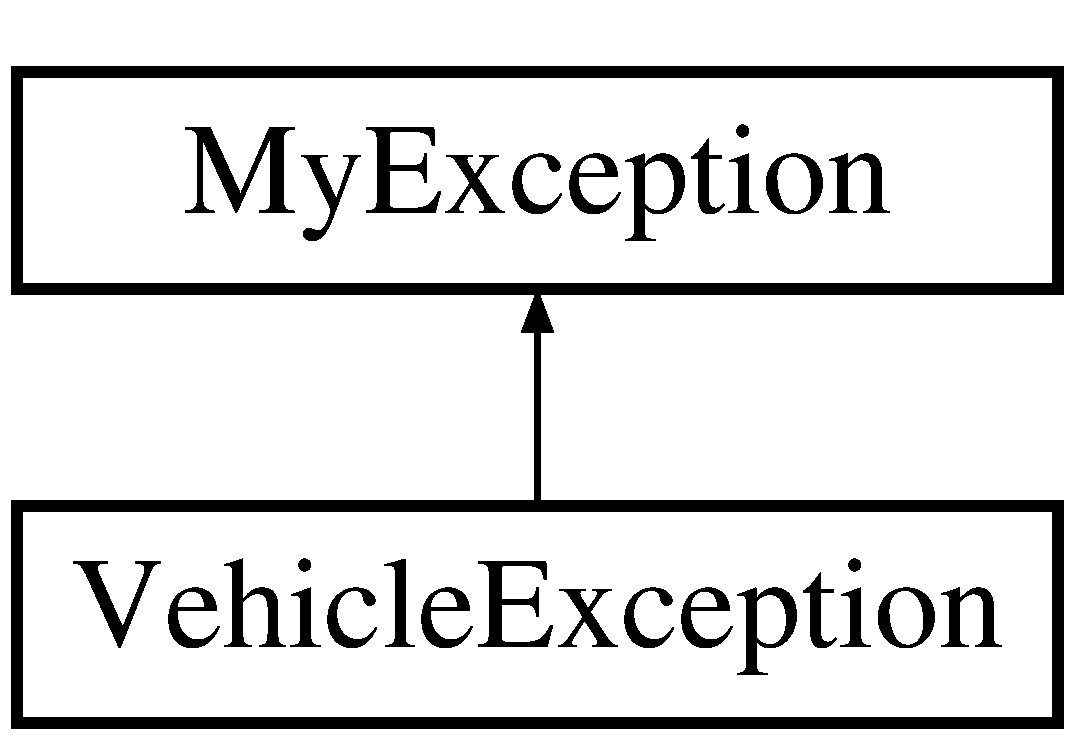
\includegraphics[height=2.000000cm]{class_vehicle_exception}
\end{center}
\end{figure}
\subsection*{Metody publiczne}
\begin{DoxyCompactItemize}
\item 
\hyperlink{class_vehicle_exception_a59ee8125aa8f15cc97951620c0c0b3b1}{Vehicle\-Exception} (string msg\-\_\-)
\end{DoxyCompactItemize}
\subsection*{Dodatkowe Dziedziczone Składowe}


\subsection{Opis szczegółowy}
Klasa wyjątku powstającego przy nieudanych operacjach na pojazdach. 

\subsection{Dokumentacja konstruktora i destruktora}
\hypertarget{class_vehicle_exception_a59ee8125aa8f15cc97951620c0c0b3b1}{\index{Vehicle\-Exception@{Vehicle\-Exception}!Vehicle\-Exception@{Vehicle\-Exception}}
\index{Vehicle\-Exception@{Vehicle\-Exception}!VehicleException@{Vehicle\-Exception}}
\subsubsection[{Vehicle\-Exception}]{\setlength{\rightskip}{0pt plus 5cm}Vehicle\-Exception\-::\-Vehicle\-Exception (
\begin{DoxyParamCaption}
\item[{string}]{msg\-\_\-}
\end{DoxyParamCaption}
)\hspace{0.3cm}{\ttfamily [inline]}}}\label{class_vehicle_exception_a59ee8125aa8f15cc97951620c0c0b3b1}


Dokumentacja dla tej klasy została wygenerowana z pliku\-:\begin{DoxyCompactItemize}
\item 
src/\hyperlink{_exceptions_8h}{Exceptions.\-h}\end{DoxyCompactItemize}

\hypertarget{struct_vertex_info}{\section{Dokumentacja struktury Vertex\-Info}
\label{struct_vertex_info}\index{Vertex\-Info@{Vertex\-Info}}
}


{\ttfamily \#include $<$Types.\-h$>$}

\subsection*{Atrybuty publiczne}
\begin{DoxyCompactItemize}
\item 
int \hyperlink{struct_vertex_info_a9592379da7b30ae95cdc1f587bccd420}{id}
\end{DoxyCompactItemize}


\subsection{Dokumentacja atrybutów składowych}
\hypertarget{struct_vertex_info_a9592379da7b30ae95cdc1f587bccd420}{\index{Vertex\-Info@{Vertex\-Info}!id@{id}}
\index{id@{id}!VertexInfo@{Vertex\-Info}}
\subsubsection[{id}]{\setlength{\rightskip}{0pt plus 5cm}int Vertex\-Info\-::id}}\label{struct_vertex_info_a9592379da7b30ae95cdc1f587bccd420}


Dokumentacja dla tej struktury została wygenerowana z pliku\-:\begin{DoxyCompactItemize}
\item 
src/\hyperlink{_types_8h}{Types.\-h}\end{DoxyCompactItemize}

\chapter{Dokumentacja plików}
\hypertarget{_animation_8cpp}{\section{Dokumentacja pliku src/\-Animation.cpp}
\label{_animation_8cpp}\index{src/\-Animation.\-cpp@{src/\-Animation.\-cpp}}
}
{\ttfamily \#include \char`\"{}Animation.\-h\char`\"{}}\\*
{\ttfamily \#include \char`\"{}Vehicle.\-h\char`\"{}}\\*
{\ttfamily \#include \char`\"{}Scene.\-h\char`\"{}}\\*
{\ttfamily \#include \char`\"{}Constants.\-h\char`\"{}}\\*
{\ttfamily \#include \char`\"{}Pedestrian.\-h\char`\"{}}\\*
{\ttfamily \#include \char`\"{}Animation\-Waiting\-Thread.\-h\char`\"{}}\\*
{\ttfamily \#include \char`\"{}Animation\-Timer\-Thread.\-h\char`\"{}}\\*
{\ttfamily \#include $<$Q\-Graphics\-View$>$}\\*
{\ttfamily \#include $<$Q\-Mutex$>$}\\*
{\ttfamily \#include $<$Q\-Mutex\-Locker$>$}\\*
{\ttfamily \#include $<$boost/function.\-hpp$>$}\\*
{\ttfamily \#include $<$boost/bind.\-hpp$>$}\\*
{\ttfamily \#include $<$algorithm$>$}\\*

\hypertarget{_animation_8h}{\section{Dokumentacja pliku src/\-Animation.h}
\label{_animation_8h}\index{src/\-Animation.\-h@{src/\-Animation.\-h}}
}
{\ttfamily \#include \char`\"{}Types.\-h\char`\"{}}\\*
{\ttfamily \#include $<$Q\-Wait\-Condition$>$}\\*
{\ttfamily \#include $<$vector$>$}\\*
\subsection*{Komponenty}
\begin{DoxyCompactItemize}
\item 
class \hyperlink{class_animation}{Animation}
\begin{DoxyCompactList}\small\item\em Klasa odpowiadająca za trzy podstawowe wątki animacji\-: aktualizacja położenia pojazdów i pieszych, oraz wątek timera. \end{DoxyCompactList}\end{DoxyCompactItemize}

\hypertarget{_animation_timer_thread_8cpp}{\section{Dokumentacja pliku src/\-Animation\-Timer\-Thread.cpp}
\label{_animation_timer_thread_8cpp}\index{src/\-Animation\-Timer\-Thread.\-cpp@{src/\-Animation\-Timer\-Thread.\-cpp}}
}
{\ttfamily \#include \char`\"{}Animation\-Timer\-Thread.\-h\char`\"{}}\\*
{\ttfamily \#include \char`\"{}Scene.\-h\char`\"{}}\\*
{\ttfamily \#include \char`\"{}Animation.\-h\char`\"{}}\\*
{\ttfamily \#include $<$Q\-Wait\-Condition$>$}\\*
{\ttfamily \#include $<$Q\-Timer$>$}\\*
{\ttfamily \#include $<$Q\-Mutex$>$}\\*
{\ttfamily \#include $<$Q\-Mutex\-Locker$>$}\\*

\hypertarget{_animation_timer_thread_8h}{\section{Dokumentacja pliku src/\-Animation\-Timer\-Thread.h}
\label{_animation_timer_thread_8h}\index{src/\-Animation\-Timer\-Thread.\-h@{src/\-Animation\-Timer\-Thread.\-h}}
}
{\ttfamily \#include $<$Q\-Thread$>$}\\*
\subsection*{Komponenty}
\begin{DoxyCompactItemize}
\item 
class \hyperlink{class_animation_timer_thread}{Animation\-Timer\-Thread}
\begin{DoxyCompactList}\small\item\em Klasa wątku animacji. Uruchamiająca timer i wybudzająca w odpowiednich momentach wątki obliczające. \end{DoxyCompactList}\end{DoxyCompactItemize}

\hypertarget{_animation_waiting_thread_8cpp}{\section{Dokumentacja pliku src/\-Animation\-Waiting\-Thread.cpp}
\label{_animation_waiting_thread_8cpp}\index{src/\-Animation\-Waiting\-Thread.\-cpp@{src/\-Animation\-Waiting\-Thread.\-cpp}}
}
{\ttfamily \#include \char`\"{}Animation\-Waiting\-Thread.\-h\char`\"{}}\\*
{\ttfamily \#include $<$Q\-Wait\-Condition$>$}\\*
{\ttfamily \#include $<$Q\-Mutex$>$}\\*
{\ttfamily \#include $<$Q\-Mutex\-Locker$>$}\\*
{\ttfamily \#include $<$Q\-Time$>$}\\*

\hypertarget{_animation_waiting_thread_8h}{\section{Dokumentacja pliku src/\-Animation\-Waiting\-Thread.h}
\label{_animation_waiting_thread_8h}\index{src/\-Animation\-Waiting\-Thread.\-h@{src/\-Animation\-Waiting\-Thread.\-h}}
}
{\ttfamily \#include \char`\"{}Types.\-h\char`\"{}}\\*
{\ttfamily \#include $<$Q\-Thread$>$}\\*
\subsection*{Komponenty}
\begin{DoxyCompactItemize}
\item 
class \hyperlink{class_animation_waiting_thread}{Animation\-Waiting\-Thread}
\begin{DoxyCompactList}\small\item\em Klasa wątków obliczeniowych (dla Pojazdów i Pieszych). Po każdym cyklu run czeka na wybudzenie po odświerzeniu widoku. \end{DoxyCompactList}\end{DoxyCompactItemize}

\hypertarget{_camera_8cpp}{\section{Dokumentacja pliku src/\-Camera.cpp}
\label{_camera_8cpp}\index{src/\-Camera.\-cpp@{src/\-Camera.\-cpp}}
}
{\ttfamily \#include \char`\"{}Camera.\-h\char`\"{}}\\*
{\ttfamily \#include \char`\"{}Vehicle.\-h\char`\"{}}\\*
{\ttfamily \#include \char`\"{}Position.\-h\char`\"{}}\\*
{\ttfamily \#include \char`\"{}Scene.\-h\char`\"{}}\\*
{\ttfamily \#include $<$Q\-Graphics\-Ellipse\-Item$>$}\\*
{\ttfamily \#include $<$Q\-Font$>$}\\*
{\ttfamily \#include $<$cmath$>$}\\*
{\ttfamily \#include $<$vector$>$}\\*

\hypertarget{_camera_8h}{\section{Dokumentacja pliku src/\-Camera.h}
\label{_camera_8h}\index{src/\-Camera.\-h@{src/\-Camera.\-h}}
}
{\ttfamily \#include $<$Q\-Object$>$}\\*
{\ttfamily \#include $<$Q\-Time$>$}\\*
{\ttfamily \#include $<$Q\-Brush$>$}\\*
{\ttfamily \#include $<$Q\-Point\-F$>$}\\*
{\ttfamily \#include $<$Q\-Pen$>$}\\*
{\ttfamily \#include $<$Q\-String$>$}\\*
{\ttfamily \#include $<$Q\-List$>$}\\*
{\ttfamily \#include $<$Q\-Rect\-F$>$}\\*
\subsection*{Komponenty}
\begin{DoxyCompactItemize}
\item 
class \hyperlink{class_camera}{Camera}
\begin{DoxyCompactList}\small\item\em Klasa reprezentująca pojedyńczą kamerę. Odpowiada za jej rysowanie i wykrywanie obiektów. \end{DoxyCompactList}\end{DoxyCompactItemize}

\hypertarget{_camera_controller_8cpp}{\section{Dokumentacja pliku src/\-Camera\-Controller.cpp}
\label{_camera_controller_8cpp}\index{src/\-Camera\-Controller.\-cpp@{src/\-Camera\-Controller.\-cpp}}
}
{\ttfamily \#include \char`\"{}Camera\-Controller.\-h\char`\"{}}\\*
{\ttfamily \#include \char`\"{}Camera.\-h\char`\"{}}\\*
{\ttfamily \#include \char`\"{}Scene.\-h\char`\"{}}\\*
{\ttfamily \#include $<$Qt\-Core$>$}\\*
{\ttfamily \#include $<$Q\-Graphics\-Scene\-Mouse\-Event$>$}\\*
{\ttfamily \#include $<$Q\-Input\-Dialog$>$}\\*
{\ttfamily \#include $<$Q\-Point\-F$>$}\\*
{\ttfamily \#include $<$algorithm$>$}\\*

\hypertarget{_camera_controller_8h}{\section{Dokumentacja pliku src/\-Camera\-Controller.h}
\label{_camera_controller_8h}\index{src/\-Camera\-Controller.\-h@{src/\-Camera\-Controller.\-h}}
}
{\ttfamily \#include $<$Q\-Object$>$}\\*
{\ttfamily \#include $<$Q\-Point\-F$>$}\\*
{\ttfamily \#include $<$Q\-Mutex$>$}\\*
{\ttfamily \#include \char`\"{}Types.\-h\char`\"{}}\\*
{\ttfamily \#include $<$vector$>$}\\*
\subsection*{Komponenty}
\begin{DoxyCompactItemize}
\item 
class \hyperlink{class_camera_controller}{Camera\-Controller}
\begin{DoxyCompactList}\small\item\em Klasa odpowiadająca za tworzenie kamer. \end{DoxyCompactList}\end{DoxyCompactItemize}

\hypertarget{_constants_8h}{\section{Dokumentacja pliku src/\-Constants.h}
\label{_constants_8h}\index{src/\-Constants.\-h@{src/\-Constants.\-h}}
}
{\ttfamily \#include $<$string$>$}\\*
\subsection*{Zmienne}
\begin{DoxyCompactItemize}
\item 
const double \hyperlink{_constants_8h_af5b8fcdbe5830cbae5d7dfabd3322114}{E\-L\-E\-M\-E\-N\-T\-A\-L\-\_\-\-W\-I\-D\-T\-H} = 20
\item 
const double \hyperlink{_constants_8h_a4b8621202e2322adb71f953eff587d3b}{C\-R\-O\-S\-S\-\_\-\-S\-I\-Z\-E} = 6
\item 
const double \hyperlink{_constants_8h_ac4a7ae3609a77ec3f01ceae9a17f386b}{P\-A\-V\-E\-M\-E\-N\-T\-\_\-\-W\-I\-D\-T\-H} = \hyperlink{_constants_8h_af5b8fcdbe5830cbae5d7dfabd3322114}{E\-L\-E\-M\-E\-N\-T\-A\-L\-\_\-\-W\-I\-D\-T\-H} $\ast$ 0.\-75
\item 
const double \hyperlink{_constants_8h_a61fbba14300f7d98cf0631b33555d6c6}{L\-A\-N\-E\-\_\-\-W\-I\-D\-T\-H} = \hyperlink{_constants_8h_af5b8fcdbe5830cbae5d7dfabd3322114}{E\-L\-E\-M\-E\-N\-T\-A\-L\-\_\-\-W\-I\-D\-T\-H} $\ast$ 0.\-15
\item 
const double \hyperlink{_constants_8h_a3c94c6998a4f3fe4998a83518095ad9e}{S\-P\-A\-W\-N\-\_\-\-L\-E\-N\-G\-T\-H} = \hyperlink{_constants_8h_af5b8fcdbe5830cbae5d7dfabd3322114}{E\-L\-E\-M\-E\-N\-T\-A\-L\-\_\-\-W\-I\-D\-T\-H} $\ast$ 6
\item 
const double \hyperlink{_constants_8h_af04082ae5253f51f70b14fbc5eb5b964}{V\-E\-H\-I\-C\-L\-E\-\_\-\-W\-I\-D\-T\-H} = 0.\-8
\item 
const double \hyperlink{_constants_8h_aa7d3cbe5b516db9a254d2392bce746b8}{V\-E\-H\-I\-C\-L\-E\-\_\-\-C\-A\-R\-\_\-\-L\-E\-N\-G\-T\-H} = \hyperlink{_constants_8h_af5b8fcdbe5830cbae5d7dfabd3322114}{E\-L\-E\-M\-E\-N\-T\-A\-L\-\_\-\-W\-I\-D\-T\-H} $\ast$ 1.\-5
\item 
const double \hyperlink{_constants_8h_a7b2ba97d26bd8ca140652468b995c42f}{V\-E\-H\-I\-C\-L\-E\-\_\-\-T\-R\-U\-C\-K\-\_\-\-L\-E\-N\-G\-T\-H} = \hyperlink{_constants_8h_af5b8fcdbe5830cbae5d7dfabd3322114}{E\-L\-E\-M\-E\-N\-T\-A\-L\-\_\-\-W\-I\-D\-T\-H} $\ast$ 2.\-5
\item 
const double \hyperlink{_constants_8h_a38605068ea7cd138cf408305b8ceb960}{V\-E\-H\-I\-C\-L\-E\-\_\-\-L\-A\-N\-E\-\_\-\-W\-I\-D\-T\-H} = (\hyperlink{_constants_8h_af5b8fcdbe5830cbae5d7dfabd3322114}{E\-L\-E\-M\-E\-N\-T\-A\-L\-\_\-\-W\-I\-D\-T\-H} $\ast$ \hyperlink{_constants_8h_a4b8621202e2322adb71f953eff587d3b}{C\-R\-O\-S\-S\-\_\-\-S\-I\-Z\-E} / 2 -\/ \hyperlink{_constants_8h_ac4a7ae3609a77ec3f01ceae9a17f386b}{P\-A\-V\-E\-M\-E\-N\-T\-\_\-\-W\-I\-D\-T\-H} -\/ \hyperlink{_constants_8h_a61fbba14300f7d98cf0631b33555d6c6}{L\-A\-N\-E\-\_\-\-W\-I\-D\-T\-H}) / 2
\item 
const int \hyperlink{_constants_8h_a04e4c5f6da15927e0c44cdb33bea2368}{V\-E\-H\-I\-C\-L\-E\-\_\-\-S\-P\-A\-W\-N\-\_\-\-I\-N\-T\-E\-R\-V\-A\-L} = 2
\item 
const double \hyperlink{_constants_8h_abaac756647b6b3e4799830825620bfbe}{P\-E\-D\-E\-S\-T\-R\-I\-A\-N\-\_\-\-R\-A\-D\-I\-U\-S} = 0.\-5 $\ast$ \hyperlink{_constants_8h_ac4a7ae3609a77ec3f01ceae9a17f386b}{P\-A\-V\-E\-M\-E\-N\-T\-\_\-\-W\-I\-D\-T\-H}
\item 
const double \hyperlink{_constants_8h_a8698aba6d49f669bea7ff13735409c16}{P\-E\-D\-E\-S\-T\-R\-I\-A\-N\-\_\-\-O\-F\-F\-S\-E\-T} = (\hyperlink{_constants_8h_ac4a7ae3609a77ec3f01ceae9a17f386b}{P\-A\-V\-E\-M\-E\-N\-T\-\_\-\-W\-I\-D\-T\-H} -\/ 2 $\ast$ \hyperlink{_constants_8h_abaac756647b6b3e4799830825620bfbe}{P\-E\-D\-E\-S\-T\-R\-I\-A\-N\-\_\-\-R\-A\-D\-I\-U\-S}) / 2
\item 
const double \hyperlink{_constants_8h_a836231bc36f1a5ad8fb66bbbf0e62c79}{P\-E\-D\-E\-S\-T\-R\-I\-A\-N\-\_\-\-S\-P\-E\-E\-D} = 20
\item 
const int \hyperlink{_constants_8h_a685dcdd84bfda84ba68dfdf78a7417b4}{N\-U\-M\-B\-E\-R\-\_\-\-O\-F\-\_\-\-P\-E\-D\-E\-S\-T\-R\-I\-A\-N\-S} = 15
\item 
const double \hyperlink{_constants_8h_a7b6696f0fad2a41a00894c598c9fb63f}{R\-O\-A\-D\-W\-A\-Y\-\_\-\-W\-I\-D\-T\-H} = (\hyperlink{_constants_8h_a4b8621202e2322adb71f953eff587d3b}{C\-R\-O\-S\-S\-\_\-\-S\-I\-Z\-E} $\ast$ \hyperlink{_constants_8h_af5b8fcdbe5830cbae5d7dfabd3322114}{E\-L\-E\-M\-E\-N\-T\-A\-L\-\_\-\-W\-I\-D\-T\-H} -\/ \hyperlink{_constants_8h_ac4a7ae3609a77ec3f01ceae9a17f386b}{P\-A\-V\-E\-M\-E\-N\-T\-\_\-\-W\-I\-D\-T\-H} $\ast$ 2)
\item 
const double \hyperlink{_constants_8h_a7c5c50f69f40c74b7b45c67aa3cd6c0a}{C\-O\-N\-S\-T\-\_\-\-D\-T} = 40
\item 
const std\-::string \hyperlink{_constants_8h_ab6d905e683157bbaadbde64a191fe341}{P\-R\-I\-O\-R\-I\-T\-Y\-\_\-\-C\-O\-L\-O\-R} = \char`\"{}white\char`\"{}
\end{DoxyCompactItemize}


\subsection{Dokumentacja zmiennych}
\hypertarget{_constants_8h_a7c5c50f69f40c74b7b45c67aa3cd6c0a}{\index{Constants.\-h@{Constants.\-h}!C\-O\-N\-S\-T\-\_\-\-D\-T@{C\-O\-N\-S\-T\-\_\-\-D\-T}}
\index{C\-O\-N\-S\-T\-\_\-\-D\-T@{C\-O\-N\-S\-T\-\_\-\-D\-T}!Constants.h@{Constants.\-h}}
\subsubsection[{C\-O\-N\-S\-T\-\_\-\-D\-T}]{\setlength{\rightskip}{0pt plus 5cm}const double C\-O\-N\-S\-T\-\_\-\-D\-T = 40}}\label{_constants_8h_a7c5c50f69f40c74b7b45c67aa3cd6c0a}
\hypertarget{_constants_8h_a4b8621202e2322adb71f953eff587d3b}{\index{Constants.\-h@{Constants.\-h}!C\-R\-O\-S\-S\-\_\-\-S\-I\-Z\-E@{C\-R\-O\-S\-S\-\_\-\-S\-I\-Z\-E}}
\index{C\-R\-O\-S\-S\-\_\-\-S\-I\-Z\-E@{C\-R\-O\-S\-S\-\_\-\-S\-I\-Z\-E}!Constants.h@{Constants.\-h}}
\subsubsection[{C\-R\-O\-S\-S\-\_\-\-S\-I\-Z\-E}]{\setlength{\rightskip}{0pt plus 5cm}const double C\-R\-O\-S\-S\-\_\-\-S\-I\-Z\-E = 6}}\label{_constants_8h_a4b8621202e2322adb71f953eff587d3b}
\hypertarget{_constants_8h_af5b8fcdbe5830cbae5d7dfabd3322114}{\index{Constants.\-h@{Constants.\-h}!E\-L\-E\-M\-E\-N\-T\-A\-L\-\_\-\-W\-I\-D\-T\-H@{E\-L\-E\-M\-E\-N\-T\-A\-L\-\_\-\-W\-I\-D\-T\-H}}
\index{E\-L\-E\-M\-E\-N\-T\-A\-L\-\_\-\-W\-I\-D\-T\-H@{E\-L\-E\-M\-E\-N\-T\-A\-L\-\_\-\-W\-I\-D\-T\-H}!Constants.h@{Constants.\-h}}
\subsubsection[{E\-L\-E\-M\-E\-N\-T\-A\-L\-\_\-\-W\-I\-D\-T\-H}]{\setlength{\rightskip}{0pt plus 5cm}const double E\-L\-E\-M\-E\-N\-T\-A\-L\-\_\-\-W\-I\-D\-T\-H = 20}}\label{_constants_8h_af5b8fcdbe5830cbae5d7dfabd3322114}
\hypertarget{_constants_8h_a61fbba14300f7d98cf0631b33555d6c6}{\index{Constants.\-h@{Constants.\-h}!L\-A\-N\-E\-\_\-\-W\-I\-D\-T\-H@{L\-A\-N\-E\-\_\-\-W\-I\-D\-T\-H}}
\index{L\-A\-N\-E\-\_\-\-W\-I\-D\-T\-H@{L\-A\-N\-E\-\_\-\-W\-I\-D\-T\-H}!Constants.h@{Constants.\-h}}
\subsubsection[{L\-A\-N\-E\-\_\-\-W\-I\-D\-T\-H}]{\setlength{\rightskip}{0pt plus 5cm}const double L\-A\-N\-E\-\_\-\-W\-I\-D\-T\-H = {\bf E\-L\-E\-M\-E\-N\-T\-A\-L\-\_\-\-W\-I\-D\-T\-H} $\ast$ 0.\-15}}\label{_constants_8h_a61fbba14300f7d98cf0631b33555d6c6}
\hypertarget{_constants_8h_a685dcdd84bfda84ba68dfdf78a7417b4}{\index{Constants.\-h@{Constants.\-h}!N\-U\-M\-B\-E\-R\-\_\-\-O\-F\-\_\-\-P\-E\-D\-E\-S\-T\-R\-I\-A\-N\-S@{N\-U\-M\-B\-E\-R\-\_\-\-O\-F\-\_\-\-P\-E\-D\-E\-S\-T\-R\-I\-A\-N\-S}}
\index{N\-U\-M\-B\-E\-R\-\_\-\-O\-F\-\_\-\-P\-E\-D\-E\-S\-T\-R\-I\-A\-N\-S@{N\-U\-M\-B\-E\-R\-\_\-\-O\-F\-\_\-\-P\-E\-D\-E\-S\-T\-R\-I\-A\-N\-S}!Constants.h@{Constants.\-h}}
\subsubsection[{N\-U\-M\-B\-E\-R\-\_\-\-O\-F\-\_\-\-P\-E\-D\-E\-S\-T\-R\-I\-A\-N\-S}]{\setlength{\rightskip}{0pt plus 5cm}const int N\-U\-M\-B\-E\-R\-\_\-\-O\-F\-\_\-\-P\-E\-D\-E\-S\-T\-R\-I\-A\-N\-S = 15}}\label{_constants_8h_a685dcdd84bfda84ba68dfdf78a7417b4}
\hypertarget{_constants_8h_ac4a7ae3609a77ec3f01ceae9a17f386b}{\index{Constants.\-h@{Constants.\-h}!P\-A\-V\-E\-M\-E\-N\-T\-\_\-\-W\-I\-D\-T\-H@{P\-A\-V\-E\-M\-E\-N\-T\-\_\-\-W\-I\-D\-T\-H}}
\index{P\-A\-V\-E\-M\-E\-N\-T\-\_\-\-W\-I\-D\-T\-H@{P\-A\-V\-E\-M\-E\-N\-T\-\_\-\-W\-I\-D\-T\-H}!Constants.h@{Constants.\-h}}
\subsubsection[{P\-A\-V\-E\-M\-E\-N\-T\-\_\-\-W\-I\-D\-T\-H}]{\setlength{\rightskip}{0pt plus 5cm}const double P\-A\-V\-E\-M\-E\-N\-T\-\_\-\-W\-I\-D\-T\-H = {\bf E\-L\-E\-M\-E\-N\-T\-A\-L\-\_\-\-W\-I\-D\-T\-H} $\ast$ 0.\-75}}\label{_constants_8h_ac4a7ae3609a77ec3f01ceae9a17f386b}
\hypertarget{_constants_8h_a8698aba6d49f669bea7ff13735409c16}{\index{Constants.\-h@{Constants.\-h}!P\-E\-D\-E\-S\-T\-R\-I\-A\-N\-\_\-\-O\-F\-F\-S\-E\-T@{P\-E\-D\-E\-S\-T\-R\-I\-A\-N\-\_\-\-O\-F\-F\-S\-E\-T}}
\index{P\-E\-D\-E\-S\-T\-R\-I\-A\-N\-\_\-\-O\-F\-F\-S\-E\-T@{P\-E\-D\-E\-S\-T\-R\-I\-A\-N\-\_\-\-O\-F\-F\-S\-E\-T}!Constants.h@{Constants.\-h}}
\subsubsection[{P\-E\-D\-E\-S\-T\-R\-I\-A\-N\-\_\-\-O\-F\-F\-S\-E\-T}]{\setlength{\rightskip}{0pt plus 5cm}const double P\-E\-D\-E\-S\-T\-R\-I\-A\-N\-\_\-\-O\-F\-F\-S\-E\-T = ({\bf P\-A\-V\-E\-M\-E\-N\-T\-\_\-\-W\-I\-D\-T\-H} -\/ 2 $\ast$ {\bf P\-E\-D\-E\-S\-T\-R\-I\-A\-N\-\_\-\-R\-A\-D\-I\-U\-S}) / 2}}\label{_constants_8h_a8698aba6d49f669bea7ff13735409c16}
\hypertarget{_constants_8h_abaac756647b6b3e4799830825620bfbe}{\index{Constants.\-h@{Constants.\-h}!P\-E\-D\-E\-S\-T\-R\-I\-A\-N\-\_\-\-R\-A\-D\-I\-U\-S@{P\-E\-D\-E\-S\-T\-R\-I\-A\-N\-\_\-\-R\-A\-D\-I\-U\-S}}
\index{P\-E\-D\-E\-S\-T\-R\-I\-A\-N\-\_\-\-R\-A\-D\-I\-U\-S@{P\-E\-D\-E\-S\-T\-R\-I\-A\-N\-\_\-\-R\-A\-D\-I\-U\-S}!Constants.h@{Constants.\-h}}
\subsubsection[{P\-E\-D\-E\-S\-T\-R\-I\-A\-N\-\_\-\-R\-A\-D\-I\-U\-S}]{\setlength{\rightskip}{0pt plus 5cm}const double P\-E\-D\-E\-S\-T\-R\-I\-A\-N\-\_\-\-R\-A\-D\-I\-U\-S = 0.\-5 $\ast$ {\bf P\-A\-V\-E\-M\-E\-N\-T\-\_\-\-W\-I\-D\-T\-H}}}\label{_constants_8h_abaac756647b6b3e4799830825620bfbe}
\hypertarget{_constants_8h_a836231bc36f1a5ad8fb66bbbf0e62c79}{\index{Constants.\-h@{Constants.\-h}!P\-E\-D\-E\-S\-T\-R\-I\-A\-N\-\_\-\-S\-P\-E\-E\-D@{P\-E\-D\-E\-S\-T\-R\-I\-A\-N\-\_\-\-S\-P\-E\-E\-D}}
\index{P\-E\-D\-E\-S\-T\-R\-I\-A\-N\-\_\-\-S\-P\-E\-E\-D@{P\-E\-D\-E\-S\-T\-R\-I\-A\-N\-\_\-\-S\-P\-E\-E\-D}!Constants.h@{Constants.\-h}}
\subsubsection[{P\-E\-D\-E\-S\-T\-R\-I\-A\-N\-\_\-\-S\-P\-E\-E\-D}]{\setlength{\rightskip}{0pt plus 5cm}const double P\-E\-D\-E\-S\-T\-R\-I\-A\-N\-\_\-\-S\-P\-E\-E\-D = 20}}\label{_constants_8h_a836231bc36f1a5ad8fb66bbbf0e62c79}
\hypertarget{_constants_8h_ab6d905e683157bbaadbde64a191fe341}{\index{Constants.\-h@{Constants.\-h}!P\-R\-I\-O\-R\-I\-T\-Y\-\_\-\-C\-O\-L\-O\-R@{P\-R\-I\-O\-R\-I\-T\-Y\-\_\-\-C\-O\-L\-O\-R}}
\index{P\-R\-I\-O\-R\-I\-T\-Y\-\_\-\-C\-O\-L\-O\-R@{P\-R\-I\-O\-R\-I\-T\-Y\-\_\-\-C\-O\-L\-O\-R}!Constants.h@{Constants.\-h}}
\subsubsection[{P\-R\-I\-O\-R\-I\-T\-Y\-\_\-\-C\-O\-L\-O\-R}]{\setlength{\rightskip}{0pt plus 5cm}const std\-::string P\-R\-I\-O\-R\-I\-T\-Y\-\_\-\-C\-O\-L\-O\-R = \char`\"{}white\char`\"{}}}\label{_constants_8h_ab6d905e683157bbaadbde64a191fe341}
\hypertarget{_constants_8h_a7b6696f0fad2a41a00894c598c9fb63f}{\index{Constants.\-h@{Constants.\-h}!R\-O\-A\-D\-W\-A\-Y\-\_\-\-W\-I\-D\-T\-H@{R\-O\-A\-D\-W\-A\-Y\-\_\-\-W\-I\-D\-T\-H}}
\index{R\-O\-A\-D\-W\-A\-Y\-\_\-\-W\-I\-D\-T\-H@{R\-O\-A\-D\-W\-A\-Y\-\_\-\-W\-I\-D\-T\-H}!Constants.h@{Constants.\-h}}
\subsubsection[{R\-O\-A\-D\-W\-A\-Y\-\_\-\-W\-I\-D\-T\-H}]{\setlength{\rightskip}{0pt plus 5cm}const double R\-O\-A\-D\-W\-A\-Y\-\_\-\-W\-I\-D\-T\-H = ({\bf C\-R\-O\-S\-S\-\_\-\-S\-I\-Z\-E} $\ast$ {\bf E\-L\-E\-M\-E\-N\-T\-A\-L\-\_\-\-W\-I\-D\-T\-H} -\/ {\bf P\-A\-V\-E\-M\-E\-N\-T\-\_\-\-W\-I\-D\-T\-H} $\ast$ 2)}}\label{_constants_8h_a7b6696f0fad2a41a00894c598c9fb63f}
\hypertarget{_constants_8h_a3c94c6998a4f3fe4998a83518095ad9e}{\index{Constants.\-h@{Constants.\-h}!S\-P\-A\-W\-N\-\_\-\-L\-E\-N\-G\-T\-H@{S\-P\-A\-W\-N\-\_\-\-L\-E\-N\-G\-T\-H}}
\index{S\-P\-A\-W\-N\-\_\-\-L\-E\-N\-G\-T\-H@{S\-P\-A\-W\-N\-\_\-\-L\-E\-N\-G\-T\-H}!Constants.h@{Constants.\-h}}
\subsubsection[{S\-P\-A\-W\-N\-\_\-\-L\-E\-N\-G\-T\-H}]{\setlength{\rightskip}{0pt plus 5cm}const double S\-P\-A\-W\-N\-\_\-\-L\-E\-N\-G\-T\-H = {\bf E\-L\-E\-M\-E\-N\-T\-A\-L\-\_\-\-W\-I\-D\-T\-H} $\ast$ 6}}\label{_constants_8h_a3c94c6998a4f3fe4998a83518095ad9e}
\hypertarget{_constants_8h_aa7d3cbe5b516db9a254d2392bce746b8}{\index{Constants.\-h@{Constants.\-h}!V\-E\-H\-I\-C\-L\-E\-\_\-\-C\-A\-R\-\_\-\-L\-E\-N\-G\-T\-H@{V\-E\-H\-I\-C\-L\-E\-\_\-\-C\-A\-R\-\_\-\-L\-E\-N\-G\-T\-H}}
\index{V\-E\-H\-I\-C\-L\-E\-\_\-\-C\-A\-R\-\_\-\-L\-E\-N\-G\-T\-H@{V\-E\-H\-I\-C\-L\-E\-\_\-\-C\-A\-R\-\_\-\-L\-E\-N\-G\-T\-H}!Constants.h@{Constants.\-h}}
\subsubsection[{V\-E\-H\-I\-C\-L\-E\-\_\-\-C\-A\-R\-\_\-\-L\-E\-N\-G\-T\-H}]{\setlength{\rightskip}{0pt plus 5cm}const double V\-E\-H\-I\-C\-L\-E\-\_\-\-C\-A\-R\-\_\-\-L\-E\-N\-G\-T\-H = {\bf E\-L\-E\-M\-E\-N\-T\-A\-L\-\_\-\-W\-I\-D\-T\-H} $\ast$ 1.\-5}}\label{_constants_8h_aa7d3cbe5b516db9a254d2392bce746b8}
\hypertarget{_constants_8h_a38605068ea7cd138cf408305b8ceb960}{\index{Constants.\-h@{Constants.\-h}!V\-E\-H\-I\-C\-L\-E\-\_\-\-L\-A\-N\-E\-\_\-\-W\-I\-D\-T\-H@{V\-E\-H\-I\-C\-L\-E\-\_\-\-L\-A\-N\-E\-\_\-\-W\-I\-D\-T\-H}}
\index{V\-E\-H\-I\-C\-L\-E\-\_\-\-L\-A\-N\-E\-\_\-\-W\-I\-D\-T\-H@{V\-E\-H\-I\-C\-L\-E\-\_\-\-L\-A\-N\-E\-\_\-\-W\-I\-D\-T\-H}!Constants.h@{Constants.\-h}}
\subsubsection[{V\-E\-H\-I\-C\-L\-E\-\_\-\-L\-A\-N\-E\-\_\-\-W\-I\-D\-T\-H}]{\setlength{\rightskip}{0pt plus 5cm}const double V\-E\-H\-I\-C\-L\-E\-\_\-\-L\-A\-N\-E\-\_\-\-W\-I\-D\-T\-H = ({\bf E\-L\-E\-M\-E\-N\-T\-A\-L\-\_\-\-W\-I\-D\-T\-H} $\ast$ {\bf C\-R\-O\-S\-S\-\_\-\-S\-I\-Z\-E} / 2 -\/ {\bf P\-A\-V\-E\-M\-E\-N\-T\-\_\-\-W\-I\-D\-T\-H} -\/ {\bf L\-A\-N\-E\-\_\-\-W\-I\-D\-T\-H}) / 2}}\label{_constants_8h_a38605068ea7cd138cf408305b8ceb960}
\hypertarget{_constants_8h_a04e4c5f6da15927e0c44cdb33bea2368}{\index{Constants.\-h@{Constants.\-h}!V\-E\-H\-I\-C\-L\-E\-\_\-\-S\-P\-A\-W\-N\-\_\-\-I\-N\-T\-E\-R\-V\-A\-L@{V\-E\-H\-I\-C\-L\-E\-\_\-\-S\-P\-A\-W\-N\-\_\-\-I\-N\-T\-E\-R\-V\-A\-L}}
\index{V\-E\-H\-I\-C\-L\-E\-\_\-\-S\-P\-A\-W\-N\-\_\-\-I\-N\-T\-E\-R\-V\-A\-L@{V\-E\-H\-I\-C\-L\-E\-\_\-\-S\-P\-A\-W\-N\-\_\-\-I\-N\-T\-E\-R\-V\-A\-L}!Constants.h@{Constants.\-h}}
\subsubsection[{V\-E\-H\-I\-C\-L\-E\-\_\-\-S\-P\-A\-W\-N\-\_\-\-I\-N\-T\-E\-R\-V\-A\-L}]{\setlength{\rightskip}{0pt plus 5cm}const int V\-E\-H\-I\-C\-L\-E\-\_\-\-S\-P\-A\-W\-N\-\_\-\-I\-N\-T\-E\-R\-V\-A\-L = 2}}\label{_constants_8h_a04e4c5f6da15927e0c44cdb33bea2368}
\hypertarget{_constants_8h_a7b2ba97d26bd8ca140652468b995c42f}{\index{Constants.\-h@{Constants.\-h}!V\-E\-H\-I\-C\-L\-E\-\_\-\-T\-R\-U\-C\-K\-\_\-\-L\-E\-N\-G\-T\-H@{V\-E\-H\-I\-C\-L\-E\-\_\-\-T\-R\-U\-C\-K\-\_\-\-L\-E\-N\-G\-T\-H}}
\index{V\-E\-H\-I\-C\-L\-E\-\_\-\-T\-R\-U\-C\-K\-\_\-\-L\-E\-N\-G\-T\-H@{V\-E\-H\-I\-C\-L\-E\-\_\-\-T\-R\-U\-C\-K\-\_\-\-L\-E\-N\-G\-T\-H}!Constants.h@{Constants.\-h}}
\subsubsection[{V\-E\-H\-I\-C\-L\-E\-\_\-\-T\-R\-U\-C\-K\-\_\-\-L\-E\-N\-G\-T\-H}]{\setlength{\rightskip}{0pt plus 5cm}const double V\-E\-H\-I\-C\-L\-E\-\_\-\-T\-R\-U\-C\-K\-\_\-\-L\-E\-N\-G\-T\-H = {\bf E\-L\-E\-M\-E\-N\-T\-A\-L\-\_\-\-W\-I\-D\-T\-H} $\ast$ 2.\-5}}\label{_constants_8h_a7b2ba97d26bd8ca140652468b995c42f}
\hypertarget{_constants_8h_af04082ae5253f51f70b14fbc5eb5b964}{\index{Constants.\-h@{Constants.\-h}!V\-E\-H\-I\-C\-L\-E\-\_\-\-W\-I\-D\-T\-H@{V\-E\-H\-I\-C\-L\-E\-\_\-\-W\-I\-D\-T\-H}}
\index{V\-E\-H\-I\-C\-L\-E\-\_\-\-W\-I\-D\-T\-H@{V\-E\-H\-I\-C\-L\-E\-\_\-\-W\-I\-D\-T\-H}!Constants.h@{Constants.\-h}}
\subsubsection[{V\-E\-H\-I\-C\-L\-E\-\_\-\-W\-I\-D\-T\-H}]{\setlength{\rightskip}{0pt plus 5cm}const double V\-E\-H\-I\-C\-L\-E\-\_\-\-W\-I\-D\-T\-H = 0.\-8}}\label{_constants_8h_af04082ae5253f51f70b14fbc5eb5b964}

\hypertarget{_cross_8cpp}{\section{Dokumentacja pliku src/\-Cross.cpp}
\label{_cross_8cpp}\index{src/\-Cross.\-cpp@{src/\-Cross.\-cpp}}
}
{\ttfamily \#include \char`\"{}Cross.\-h\char`\"{}}\\*
{\ttfamily \#include \char`\"{}Scene.\-h\char`\"{}}\\*
{\ttfamily \#include \char`\"{}Priority\-Rules.\-h\char`\"{}}\\*
{\ttfamily \#include \char`\"{}Cross\-Rules.\-h\char`\"{}}\\*
{\ttfamily \#include \char`\"{}Exceptions.\-h\char`\"{}}\\*
{\ttfamily \#include \char`\"{}Position.\-h\char`\"{}}\\*
{\ttfamily \#include $<$Q\-Brush$>$}\\*
{\ttfamily \#include $<$Q\-Pen$>$}\\*
{\ttfamily \#include $<$Q\-Time$>$}\\*
{\ttfamily \#include $<$Q\-Graphics\-Item\-Group$>$}\\*
{\ttfamily \#include $<$Q\-Graphics\-Ellipse\-Item$>$}\\*
{\ttfamily \#include $<$Q\-String$>$}\\*
{\ttfamily \#include $<$boost/bind.\-hpp$>$}\\*
{\ttfamily \#include $<$algorithm$>$}\\*
{\ttfamily \#include $<$set$>$}\\*

\hypertarget{_cross_8h}{\section{Dokumentacja pliku src/\-Cross.h}
\label{_cross_8h}\index{src/\-Cross.\-h@{src/\-Cross.\-h}}
}
{\ttfamily \#include \char`\"{}Map\-Element.\-h\char`\"{}}\\*
{\ttfamily \#include \char`\"{}Types.\-h\char`\"{}}\\*
{\ttfamily \#include \char`\"{}Constants.\-h\char`\"{}}\\*
{\ttfamily \#include \char`\"{}Direction.\-h\char`\"{}}\\*
{\ttfamily \#include $<$map$>$}\\*
{\ttfamily \#include $<$vector$>$}\\*
\subsection*{Komponenty}
\begin{DoxyCompactItemize}
\item 
class \hyperlink{class_cross}{Cross}
\begin{DoxyCompactList}\small\item\em Klasa reprezentujaca skrzyzowanie. \end{DoxyCompactList}\end{DoxyCompactItemize}

\hypertarget{_cross_rules_8cpp}{\section{Dokumentacja pliku src/\-Cross\-Rules.cpp}
\label{_cross_rules_8cpp}\index{src/\-Cross\-Rules.\-cpp@{src/\-Cross\-Rules.\-cpp}}
}
{\ttfamily \#include \char`\"{}Cross\-Rules.\-h\char`\"{}}\\*
{\ttfamily \#include \char`\"{}Exceptions.\-h\char`\"{}}\\*
{\ttfamily \#include $<$algorithm$>$}\\*
{\ttfamily \#include $<$boost/lambda/lambda.\-hpp$>$}\\*
{\ttfamily \#include $<$boost/bind.\-hpp$>$}\\*

\hypertarget{_cross_rules_8h}{\section{Dokumentacja pliku src/\-Cross\-Rules.h}
\label{_cross_rules_8h}\index{src/\-Cross\-Rules.\-h@{src/\-Cross\-Rules.\-h}}
}
{\ttfamily \#include \char`\"{}Priority\-Rules.\-h\char`\"{}}\\*
{\ttfamily \#include \char`\"{}Direction.\-h\char`\"{}}\\*
{\ttfamily \#include $<$map$>$}\\*
{\ttfamily \#include $<$vector$>$}\\*
{\ttfamily \#include $<$set$>$}\\*
\subsection*{Komponenty}
\begin{DoxyCompactItemize}
\item 
class \hyperlink{class_cross_rules}{Cross\-Rules}
\begin{DoxyCompactList}\small\item\em Klasa podająca informacje o pierwszeństwie przejazdu. \end{DoxyCompactList}\end{DoxyCompactItemize}

\hypertarget{_direction_8h}{\section{Dokumentacja pliku src/\-Direction.h}
\label{_direction_8h}\index{src/\-Direction.\-h@{src/\-Direction.\-h}}
}
\subsection*{Wyliczenia}
\begin{DoxyCompactItemize}
\item 
enum \hyperlink{_direction_8h_a224b9163917ac32fc95a60d8c1eec3aa}{Direction} \{ \hyperlink{_direction_8h_a224b9163917ac32fc95a60d8c1eec3aaa2c63acbe79d9f41ba6bb7766e9c37702}{N} =  0, 
\hyperlink{_direction_8h_a224b9163917ac32fc95a60d8c1eec3aaab199e021998d49b1f09338d8b9b18ecb}{E} =  1, 
\hyperlink{_direction_8h_a224b9163917ac32fc95a60d8c1eec3aaaf1ce01387d2348f8b858721a7db81670}{S} =  2, 
\hyperlink{_direction_8h_a224b9163917ac32fc95a60d8c1eec3aaab722ceeb601c72cd78fbd35f3581fdf7}{W} =  3
 \}
\begin{DoxyCompactList}\small\item\em Typ wyliczeniowy do określania kierunków. \end{DoxyCompactList}\end{DoxyCompactItemize}


\subsection{Dokumentacja typów wyliczanych}
\hypertarget{_direction_8h_a224b9163917ac32fc95a60d8c1eec3aa}{\index{Direction.\-h@{Direction.\-h}!Direction@{Direction}}
\index{Direction@{Direction}!Direction.h@{Direction.\-h}}
\subsubsection[{Direction}]{\setlength{\rightskip}{0pt plus 5cm}enum {\bf Direction}}}\label{_direction_8h_a224b9163917ac32fc95a60d8c1eec3aa}


Typ wyliczeniowy do określania kierunków. 

\hyperlink{_direction_8h}{Direction.\-h} Wyliczenie możliwych kierunków przemieszczania się elementów animacji. Możliwie kierunki to odpowiednio\-: północ, wschód, południe , zachód. \begin{Desc}
\item[Wartości wyliczeń\-: ]\par
\begin{description}
\index{N@{N}!Direction.\-h@{Direction.\-h}}\index{Direction.\-h@{Direction.\-h}!N@{N}}\item[{\em 
\hypertarget{_direction_8h_a224b9163917ac32fc95a60d8c1eec3aaa2c63acbe79d9f41ba6bb7766e9c37702}{N}\label{_direction_8h_a224b9163917ac32fc95a60d8c1eec3aaa2c63acbe79d9f41ba6bb7766e9c37702}
}]\index{E@{E}!Direction.\-h@{Direction.\-h}}\index{Direction.\-h@{Direction.\-h}!E@{E}}\item[{\em 
\hypertarget{_direction_8h_a224b9163917ac32fc95a60d8c1eec3aaab199e021998d49b1f09338d8b9b18ecb}{E}\label{_direction_8h_a224b9163917ac32fc95a60d8c1eec3aaab199e021998d49b1f09338d8b9b18ecb}
}]\index{S@{S}!Direction.\-h@{Direction.\-h}}\index{Direction.\-h@{Direction.\-h}!S@{S}}\item[{\em 
\hypertarget{_direction_8h_a224b9163917ac32fc95a60d8c1eec3aaaf1ce01387d2348f8b858721a7db81670}{S}\label{_direction_8h_a224b9163917ac32fc95a60d8c1eec3aaaf1ce01387d2348f8b858721a7db81670}
}]\index{W@{W}!Direction.\-h@{Direction.\-h}}\index{Direction.\-h@{Direction.\-h}!W@{W}}\item[{\em 
\hypertarget{_direction_8h_a224b9163917ac32fc95a60d8c1eec3aaab722ceeb601c72cd78fbd35f3581fdf7}{W}\label{_direction_8h_a224b9163917ac32fc95a60d8c1eec3aaab722ceeb601c72cd78fbd35f3581fdf7}
}]\end{description}
\end{Desc}


\hypertarget{_drawable_8h}{\section{Dokumentacja pliku src/\-Drawable.h}
\label{_drawable_8h}\index{src/\-Drawable.\-h@{src/\-Drawable.\-h}}
}
{\ttfamily \#include \char`\"{}Position.\-h\char`\"{}}\\*
\subsection*{Komponenty}
\begin{DoxyCompactItemize}
\item 
class \hyperlink{class_drawable}{Drawable}
\begin{DoxyCompactList}\small\item\em Klasa bazowa dla obiektów, które będą wyświetlane na scenie. \end{DoxyCompactList}\end{DoxyCompactItemize}

\hypertarget{_exceptions_8h}{\section{Dokumentacja pliku src/\-Exceptions.h}
\label{_exceptions_8h}\index{src/\-Exceptions.\-h@{src/\-Exceptions.\-h}}
}
{\ttfamily \#include $<$exception$>$}\\*
{\ttfamily \#include $<$string$>$}\\*
\subsection*{Komponenty}
\begin{DoxyCompactItemize}
\item 
class \hyperlink{class_my_exception}{My\-Exception}
\begin{DoxyCompactList}\small\item\em Klasa bazowa dla tworzonych w aplikacji wyjątków. \end{DoxyCompactList}\item 
class \hyperlink{class_map_exception}{Map\-Exception}
\begin{DoxyCompactList}\small\item\em Klasa wyjątku powstającego przy nieudanym tworzeniu mapy. \end{DoxyCompactList}\item 
class \hyperlink{class_vehicle_exception}{Vehicle\-Exception}
\begin{DoxyCompactList}\small\item\em Klasa wyjątku powstającego przy nieudanych operacjach na pojazdach. \end{DoxyCompactList}\end{DoxyCompactItemize}

\hypertarget{main_8cpp}{\section{Dokumentacja pliku src/main.cpp}
\label{main_8cpp}\index{src/main.\-cpp@{src/main.\-cpp}}
}
{\ttfamily \#include \char`\"{}Main\-Window.\-h\char`\"{}}\\*
{\ttfamily \#include $<$Q\-Application$>$}\\*
{\ttfamily \#include \char`\"{}Exceptions.\-h\char`\"{}}\\*
\subsection*{Funkcje}
\begin{DoxyCompactItemize}
\item 
int \hyperlink{main_8cpp_a0ddf1224851353fc92bfbff6f499fa97}{main} (int argc, char $\ast$argv\mbox{[}$\,$\mbox{]})
\end{DoxyCompactItemize}


\subsection{Dokumentacja funkcji}
\hypertarget{main_8cpp_a0ddf1224851353fc92bfbff6f499fa97}{\index{main.\-cpp@{main.\-cpp}!main@{main}}
\index{main@{main}!main.cpp@{main.\-cpp}}
\subsubsection[{main}]{\setlength{\rightskip}{0pt plus 5cm}int main (
\begin{DoxyParamCaption}
\item[{int}]{argc, }
\item[{char $\ast$}]{argv\mbox{[}$\,$\mbox{]}}
\end{DoxyParamCaption}
)}}\label{main_8cpp_a0ddf1224851353fc92bfbff6f499fa97}

\hypertarget{_main_window_8cpp}{\section{Dokumentacja pliku src/\-Main\-Window.cpp}
\label{_main_window_8cpp}\index{src/\-Main\-Window.\-cpp@{src/\-Main\-Window.\-cpp}}
}
{\ttfamily \#include \char`\"{}Main\-Window.\-h\char`\"{}}\\*
{\ttfamily \#include \char`\"{}Scene.\-h\char`\"{}}\\*
{\ttfamily \#include \char`\"{}Simulator.\-h\char`\"{}}\\*
{\ttfamily \#include \char`\"{}Camera\-Controller.\-h\char`\"{}}\\*
{\ttfamily \#include \char`\"{}Exceptions.\-h\char`\"{}}\\*
{\ttfamily \#include $<$Q\-Time$>$}\\*
{\ttfamily \#include $<$Q\-Grid\-Layout$>$}\\*
{\ttfamily \#include $<$Q\-Push\-Button$>$}\\*
{\ttfamily \#include $<$Q\-Graphics\-View$>$}\\*
{\ttfamily \#include $<$Q\-Text\-Edit$>$}\\*
{\ttfamily \#include $<$Q\-Message\-Box$>$}\\*
{\ttfamily \#include $<$Q\-File\-Dialog$>$}\\*
{\ttfamily \#include $<$fstream$>$}\\*

\hypertarget{_main_window_8h}{\section{Dokumentacja pliku src/\-Main\-Window.h}
\label{_main_window_8h}\index{src/\-Main\-Window.\-h@{src/\-Main\-Window.\-h}}
}
{\ttfamily \#include $<$Q\-Widget$>$}\\*
\subsection*{Komponenty}
\begin{DoxyCompactItemize}
\item 
class \hyperlink{class_main_window}{Main\-Window}
\begin{DoxyCompactList}\small\item\em Klasa głównego okna aplikacji. \end{DoxyCompactList}\end{DoxyCompactItemize}

\hypertarget{_map_element_8h}{\section{Dokumentacja pliku src/\-Map\-Element.h}
\label{_map_element_8h}\index{src/\-Map\-Element.\-h@{src/\-Map\-Element.\-h}}
}
{\ttfamily \#include \char`\"{}Drawable.\-h\char`\"{}}\\*
\subsection*{Komponenty}
\begin{DoxyCompactItemize}
\item 
class \hyperlink{class_map_element}{Map\-Element}
\begin{DoxyCompactList}\small\item\em Klasa bazowa dla Drogi, Skrzyżowania i miejsc tworzenia pojazdów. \end{DoxyCompactList}\end{DoxyCompactItemize}

\hypertarget{_map_factory_8cpp}{\section{Dokumentacja pliku src/\-Map\-Factory.cpp}
\label{_map_factory_8cpp}\index{src/\-Map\-Factory.\-cpp@{src/\-Map\-Factory.\-cpp}}
}
{\ttfamily \#include \char`\"{}Map\-Factory.\-h\char`\"{}}\\*
{\ttfamily \#include \char`\"{}Scene.\-h\char`\"{}}\\*
{\ttfamily \#include \char`\"{}Spawn.\-h\char`\"{}}\\*
{\ttfamily \#include \char`\"{}Cross.\-h\char`\"{}}\\*
{\ttfamily \#include \char`\"{}Cross\-Rules.\-h\char`\"{}}\\*
{\ttfamily \#include \char`\"{}Exceptions.\-h\char`\"{}}\\*
{\ttfamily \#include \char`\"{}Constants.\-h\char`\"{}}\\*
{\ttfamily \#include $<$exception$>$}\\*
{\ttfamily \#include $<$boost/property\-\_\-tree/json\-\_\-parser.\-hpp$>$}\\*
{\ttfamily \#include $<$boost/property\-\_\-tree/detail/json\-\_\-parser\-\_\-error.\-hpp$>$}\\*
{\ttfamily \#include $<$boost/foreach.\-hpp$>$}\\*
{\ttfamily \#include $<$sstream$>$}\\*
\subsection*{Definicje typów}
\begin{DoxyCompactItemize}
\item 
typedef boost\-::graph\-\_\-traits\\*
$<$ \hyperlink{_types_8h_adb8cbccb1bf63dda03515e30e185c388}{Graph} $>$\-::vertex\-\_\-iterator \hyperlink{_map_factory_8cpp_ae6603b1d73e6c4cf70f33b356e8d591c}{Vertex\-Iterator}
\item 
typedef boost\-::property\-\_\-map\\*
$<$ \hyperlink{_types_8h_adb8cbccb1bf63dda03515e30e185c388}{Graph}, boost\-::vertex\-\_\-index\-\_\-t $>$\\*
\-::type \hyperlink{_map_factory_8cpp_a60e573ea64bc6383ce20314f49c90c8c}{Index\-Map}
\end{DoxyCompactItemize}


\subsection{Dokumentacja definicji typów}
\hypertarget{_map_factory_8cpp_a60e573ea64bc6383ce20314f49c90c8c}{\index{Map\-Factory.\-cpp@{Map\-Factory.\-cpp}!Index\-Map@{Index\-Map}}
\index{Index\-Map@{Index\-Map}!MapFactory.cpp@{Map\-Factory.\-cpp}}
\subsubsection[{Index\-Map}]{\setlength{\rightskip}{0pt plus 5cm}typedef boost\-::property\-\_\-map$<${\bf Graph}, boost\-::vertex\-\_\-index\-\_\-t $>$\-::type {\bf Index\-Map}}}\label{_map_factory_8cpp_a60e573ea64bc6383ce20314f49c90c8c}
\hypertarget{_map_factory_8cpp_ae6603b1d73e6c4cf70f33b356e8d591c}{\index{Map\-Factory.\-cpp@{Map\-Factory.\-cpp}!Vertex\-Iterator@{Vertex\-Iterator}}
\index{Vertex\-Iterator@{Vertex\-Iterator}!MapFactory.cpp@{Map\-Factory.\-cpp}}
\subsubsection[{Vertex\-Iterator}]{\setlength{\rightskip}{0pt plus 5cm}typedef boost\-::graph\-\_\-traits$<${\bf Graph}$>$\-::vertex\-\_\-iterator {\bf Vertex\-Iterator}}}\label{_map_factory_8cpp_ae6603b1d73e6c4cf70f33b356e8d591c}

\hypertarget{_map_factory_8h}{\section{Dokumentacja pliku src/\-Map\-Factory.h}
\label{_map_factory_8h}\index{src/\-Map\-Factory.\-h@{src/\-Map\-Factory.\-h}}
}
{\ttfamily \#include \char`\"{}Direction.\-h\char`\"{}}\\*
{\ttfamily \#include \char`\"{}Map\-Element.\-h\char`\"{}}\\*
{\ttfamily \#include \char`\"{}Types.\-h\char`\"{}}\\*
{\ttfamily \#include $<$boost/property\-\_\-tree/ptree.\-hpp$>$}\\*
{\ttfamily \#include $<$map$>$}\\*
{\ttfamily \#include $<$vector$>$}\\*
{\ttfamily \#include $<$string$>$}\\*
\subsection*{Komponenty}
\begin{DoxyCompactItemize}
\item 
class \hyperlink{class_map_factory}{Map\-Factory}
\begin{DoxyCompactList}\small\item\em Klasa odpowiada za czytanie pliku w formacie json i tworzenie na jego podstawie grafu i wszystkich elementów mapy. \end{DoxyCompactList}\end{DoxyCompactItemize}
\subsection*{Definicje typów}
\begin{DoxyCompactItemize}
\item 
typedef boost\-::property\-\_\-tree\-::ptree \hyperlink{_map_factory_8h_a54a98738cc1e3485f2cf5f24979317e5}{ptree}
\end{DoxyCompactItemize}


\subsection{Dokumentacja definicji typów}
\hypertarget{_map_factory_8h_a54a98738cc1e3485f2cf5f24979317e5}{\index{Map\-Factory.\-h@{Map\-Factory.\-h}!ptree@{ptree}}
\index{ptree@{ptree}!MapFactory.h@{Map\-Factory.\-h}}
\subsubsection[{ptree}]{\setlength{\rightskip}{0pt plus 5cm}typedef boost\-::property\-\_\-tree\-::ptree {\bf ptree}}}\label{_map_factory_8h_a54a98738cc1e3485f2cf5f24979317e5}

\hypertarget{_moveable_8h}{\section{Dokumentacja pliku src/\-Moveable.h}
\label{_moveable_8h}\index{src/\-Moveable.\-h@{src/\-Moveable.\-h}}
}
{\ttfamily \#include \char`\"{}Direction.\-h\char`\"{}}\\*
\subsection*{Komponenty}
\begin{DoxyCompactItemize}
\item 
class \hyperlink{class_moveable}{Moveable}
\begin{DoxyCompactList}\small\item\em Klasa bazowa dla klas, które będą animowane. \end{DoxyCompactList}\end{DoxyCompactItemize}

\hypertarget{_pedestrian_8cpp}{\section{Dokumentacja pliku src/\-Pedestrian.cpp}
\label{_pedestrian_8cpp}\index{src/\-Pedestrian.\-cpp@{src/\-Pedestrian.\-cpp}}
}
{\ttfamily \#include \char`\"{}Pedestrian.\-h\char`\"{}}\\*
{\ttfamily \#include \char`\"{}Constants.\-h\char`\"{}}\\*
{\ttfamily \#include \char`\"{}Scene.\-h\char`\"{}}\\*
{\ttfamily \#include \char`\"{}Cross.\-h\char`\"{}}\\*
{\ttfamily \#include \char`\"{}Spawn.\-h\char`\"{}}\\*
{\ttfamily \#include \char`\"{}Position.\-h\char`\"{}}\\*
{\ttfamily \#include $<$cmath$>$}\\*

\hypertarget{_pedestrian_8h}{\section{Dokumentacja pliku src/\-Pedestrian.h}
\label{_pedestrian_8h}\index{src/\-Pedestrian.\-h@{src/\-Pedestrian.\-h}}
}
{\ttfamily \#include \char`\"{}Moveable.\-h\char`\"{}}\\*
{\ttfamily \#include \char`\"{}Drawable.\-h\char`\"{}}\\*
{\ttfamily \#include $<$Q\-Color$>$}\\*
{\ttfamily \#include $<$Q\-Graphics\-Ellipse\-Item$>$}\\*
{\ttfamily \#include $<$vector$>$}\\*
\subsection*{Komponenty}
\begin{DoxyCompactItemize}
\item 
class \hyperlink{class_pedestrian}{Pedestrian}
\begin{DoxyCompactList}\small\item\em Klasa reprezentująca pieszego. \end{DoxyCompactList}\end{DoxyCompactItemize}

\hypertarget{_position_8h}{\section{Dokumentacja pliku src/\-Position.h}
\label{_position_8h}\index{src/\-Position.\-h@{src/\-Position.\-h}}
}
{\ttfamily \#include \char`\"{}Constants.\-h\char`\"{}}\\*
\subsection*{Komponenty}
\begin{DoxyCompactItemize}
\item 
struct \hyperlink{struct_position}{Position}
\begin{DoxyCompactList}\small\item\em Klasa reprezentuje punkt w trójwymiarowej przestrzeni. \end{DoxyCompactList}\end{DoxyCompactItemize}

\hypertarget{_priority_rules_8h}{\section{Dokumentacja pliku src/\-Priority\-Rules.h}
\label{_priority_rules_8h}\index{src/\-Priority\-Rules.\-h@{src/\-Priority\-Rules.\-h}}
}
{\ttfamily \#include \char`\"{}Direction.\-h\char`\"{}}\\*
{\ttfamily \#include $<$set$>$}\\*
\subsection*{Komponenty}
\begin{DoxyCompactItemize}
\item 
class \hyperlink{class_priority_rules}{Priority\-Rules}
\begin{DoxyCompactList}\small\item\em Klasa bazowa dla \hyperlink{class_cross_rules}{Cross\-Rules}. Dwustopniowa herarchia klas umożliwia późniejszy rozwój. Np. dodanie sygnalizacji świetlnej. \end{DoxyCompactList}\end{DoxyCompactItemize}

\hypertarget{_road_8cpp}{\section{Dokumentacja pliku src/\-Road.cpp}
\label{_road_8cpp}\index{src/\-Road.\-cpp@{src/\-Road.\-cpp}}
}
{\ttfamily \#include \char`\"{}Road.\-h\char`\"{}}\\*
{\ttfamily \#include \char`\"{}Scene.\-h\char`\"{}}\\*
{\ttfamily \#include \char`\"{}Constants.\-h\char`\"{}}\\*
{\ttfamily \#include \char`\"{}Exceptions.\-h\char`\"{}}\\*
{\ttfamily \#include $<$Q\-Graphics\-Item\-Group$>$}\\*
{\ttfamily \#include $<$Q\-Brush$>$}\\*
{\ttfamily \#include $<$Q\-Pen$>$}\\*
{\ttfamily \#include $<$Q\-Graphics\-Rect\-Item$>$}\\*
{\ttfamily \#include $<$Q\-Graphics\-Line\-Item$>$}\\*

\hypertarget{_road_8h}{\section{Dokumentacja pliku src/\-Road.h}
\label{_road_8h}\index{src/\-Road.\-h@{src/\-Road.\-h}}
}
{\ttfamily \#include \char`\"{}Map\-Element.\-h\char`\"{}}\\*
{\ttfamily \#include \char`\"{}Direction.\-h\char`\"{}}\\*
{\ttfamily \#include \char`\"{}Types.\-h\char`\"{}}\\*
\subsection*{Komponenty}
\begin{DoxyCompactItemize}
\item 
class \hyperlink{class_road}{Road}
\begin{DoxyCompactList}\small\item\em Klasa reprezentuje drogę na mapie. \end{DoxyCompactList}\end{DoxyCompactItemize}

\hypertarget{_scene_8cpp}{\section{Dokumentacja pliku src/\-Scene.cpp}
\label{_scene_8cpp}\index{src/\-Scene.\-cpp@{src/\-Scene.\-cpp}}
}
{\ttfamily \#include \char`\"{}Scene.\-h\char`\"{}}\\*
{\ttfamily \#include \char`\"{}Main\-Window.\-h\char`\"{}}\\*
{\ttfamily \#include \char`\"{}Constants.\-h\char`\"{}}\\*
{\ttfamily \#include \char`\"{}Camera\-Controller.\-h\char`\"{}}\\*
{\ttfamily \#include \char`\"{}Vehicle.\-h\char`\"{}}\\*
{\ttfamily \#include \char`\"{}Pedestrian.\-h\char`\"{}}\\*
{\ttfamily \#include \char`\"{}Map\-Factory.\-h\char`\"{}}\\*
{\ttfamily \#include $<$Q\-List$>$}\\*
{\ttfamily \#include $<$Q\-List\-Iterator$>$}\\*
{\ttfamily \#include $<$Q\-Graphics\-Item$>$}\\*
{\ttfamily \#include $<$Q\-Variant$>$}\\*
{\ttfamily \#include $<$Q\-Mutex\-Locker$>$}\\*

\hypertarget{_scene_8h}{\section{Dokumentacja pliku src/\-Scene.h}
\label{_scene_8h}\index{src/\-Scene.\-h@{src/\-Scene.\-h}}
}
{\ttfamily \#include \char`\"{}Types.\-h\char`\"{}}\\*
{\ttfamily \#include \char`\"{}Animation.\-h\char`\"{}}\\*
{\ttfamily \#include \char`\"{}Shortest\-Path.\-h\char`\"{}}\\*
{\ttfamily \#include \char`\"{}Cross.\-h\char`\"{}}\\*
{\ttfamily \#include \char`\"{}Road.\-h\char`\"{}}\\*
{\ttfamily \#include \char`\"{}Spawn.\-h\char`\"{}}\\*
{\ttfamily \#include $<$Qt\-Core$>$}\\*
{\ttfamily \#include $<$Q\-Graphics\-View$>$}\\*
{\ttfamily \#include $<$Q\-Graphics\-Scene$>$}\\*
{\ttfamily \#include $<$Q\-Widget$>$}\\*
{\ttfamily \#include $<$Q\-Brush$>$}\\*
{\ttfamily \#include $<$Q\-Pen$>$}\\*
{\ttfamily \#include $<$Q\-Wait\-Condition$>$}\\*
{\ttfamily \#include $<$vector$>$}\\*
{\ttfamily \#include $<$string$>$}\\*
\subsection*{Komponenty}
\begin{DoxyCompactItemize}
\item 
class \hyperlink{class_scene}{Scene}
\begin{DoxyCompactList}\small\item\em Klasa odpowiadająca za graficzną prezentację symulacji, dziedziczy po Q\-Graphics\-Scene i rysuje poszczególne elementy. \end{DoxyCompactList}\end{DoxyCompactItemize}

\hypertarget{_shortest_path_8cpp}{\section{Dokumentacja pliku src/\-Shortest\-Path.cpp}
\label{_shortest_path_8cpp}\index{src/\-Shortest\-Path.\-cpp@{src/\-Shortest\-Path.\-cpp}}
}
{\ttfamily \#include \char`\"{}Shortest\-Path.\-h\char`\"{}}\\*
{\ttfamily \#include \char`\"{}Exceptions.\-h\char`\"{}}\\*
{\ttfamily \#include $<$boost/graph/dijkstra\-\_\-shortest\-\_\-paths.\-hpp$>$}\\*
{\ttfamily \#include $<$utility$>$}\\*

\hypertarget{_shortest_path_8h}{\section{Dokumentacja pliku src/\-Shortest\-Path.h}
\label{_shortest_path_8h}\index{src/\-Shortest\-Path.\-h@{src/\-Shortest\-Path.\-h}}
}
{\ttfamily \#include \char`\"{}Types.\-h\char`\"{}}\\*
{\ttfamily \#include $<$vector$>$}\\*
\subsection*{Komponenty}
\begin{DoxyCompactItemize}
\item 
class \hyperlink{class_shortest_path}{Shortest\-Path}
\begin{DoxyCompactList}\small\item\em Klasa odpowiadająca za wyznaczanie najkrótszej ścieżki pomiędzy elementami o podanych I\-D. \end{DoxyCompactList}\end{DoxyCompactItemize}
\subsection*{Definicje typów}
\begin{DoxyCompactItemize}
\item 
typedef boost\-::graph\-\_\-traits\\*
$<$ \hyperlink{_types_8h_adb8cbccb1bf63dda03515e30e185c388}{Graph} $>$\-::vertex\-\_\-iterator \hyperlink{_shortest_path_8h_ae6603b1d73e6c4cf70f33b356e8d591c}{Vertex\-Iterator}
\item 
typedef boost\-::property\-\_\-map\\*
$<$ \hyperlink{_types_8h_adb8cbccb1bf63dda03515e30e185c388}{Graph}, boost\-::vertex\-\_\-index\-\_\-t $>$\\*
\-::type \hyperlink{_shortest_path_8h_a60e573ea64bc6383ce20314f49c90c8c}{Index\-Map}
\item 
typedef \\*
boost\-::iterator\-\_\-property\-\_\-map\\*
$<$ \hyperlink{_types_8h_a8c93f604acf57e6a9bae1f91c379ac98}{Vertex} $\ast$, \hyperlink{_map_factory_8cpp_a60e573ea64bc6383ce20314f49c90c8c}{Index\-Map}, \hyperlink{_types_8h_a8c93f604acf57e6a9bae1f91c379ac98}{Vertex}, \\*
\hyperlink{_types_8h_a8c93f604acf57e6a9bae1f91c379ac98}{Vertex} \& $>$ \hyperlink{_shortest_path_8h_ae20d582e38f0013afe10a82c1a12cb4f}{Predecessor\-Map}
\item 
typedef \\*
boost\-::iterator\-\_\-property\-\_\-map\\*
$<$ \hyperlink{_types_8h_aa4dd30204ac53d8c88cfd0cab7b81789}{Weight} $\ast$, \hyperlink{_map_factory_8cpp_a60e573ea64bc6383ce20314f49c90c8c}{Index\-Map}, \hyperlink{_types_8h_aa4dd30204ac53d8c88cfd0cab7b81789}{Weight}, \\*
\hyperlink{_types_8h_aa4dd30204ac53d8c88cfd0cab7b81789}{Weight} \& $>$ \hyperlink{_shortest_path_8h_acab893c91ba1c4e4415b652ccebeea6a}{Distance\-Map}
\end{DoxyCompactItemize}


\subsection{Dokumentacja definicji typów}
\hypertarget{_shortest_path_8h_acab893c91ba1c4e4415b652ccebeea6a}{\index{Shortest\-Path.\-h@{Shortest\-Path.\-h}!Distance\-Map@{Distance\-Map}}
\index{Distance\-Map@{Distance\-Map}!ShortestPath.h@{Shortest\-Path.\-h}}
\subsubsection[{Distance\-Map}]{\setlength{\rightskip}{0pt plus 5cm}typedef boost\-::iterator\-\_\-property\-\_\-map$<$ {\bf Weight}$\ast$, {\bf Index\-Map}, {\bf Weight}, {\bf Weight}\& $>$ {\bf Distance\-Map}}}\label{_shortest_path_8h_acab893c91ba1c4e4415b652ccebeea6a}
\hypertarget{_shortest_path_8h_a60e573ea64bc6383ce20314f49c90c8c}{\index{Shortest\-Path.\-h@{Shortest\-Path.\-h}!Index\-Map@{Index\-Map}}
\index{Index\-Map@{Index\-Map}!ShortestPath.h@{Shortest\-Path.\-h}}
\subsubsection[{Index\-Map}]{\setlength{\rightskip}{0pt plus 5cm}typedef boost\-::property\-\_\-map$<${\bf Graph}, boost\-::vertex\-\_\-index\-\_\-t $>$\-::type {\bf Index\-Map}}}\label{_shortest_path_8h_a60e573ea64bc6383ce20314f49c90c8c}
\hypertarget{_shortest_path_8h_ae20d582e38f0013afe10a82c1a12cb4f}{\index{Shortest\-Path.\-h@{Shortest\-Path.\-h}!Predecessor\-Map@{Predecessor\-Map}}
\index{Predecessor\-Map@{Predecessor\-Map}!ShortestPath.h@{Shortest\-Path.\-h}}
\subsubsection[{Predecessor\-Map}]{\setlength{\rightskip}{0pt plus 5cm}typedef boost\-::iterator\-\_\-property\-\_\-map$<$ {\bf Vertex}$\ast$, {\bf Index\-Map}, {\bf Vertex}, {\bf Vertex}\& $>$ {\bf Predecessor\-Map}}}\label{_shortest_path_8h_ae20d582e38f0013afe10a82c1a12cb4f}
\hypertarget{_shortest_path_8h_ae6603b1d73e6c4cf70f33b356e8d591c}{\index{Shortest\-Path.\-h@{Shortest\-Path.\-h}!Vertex\-Iterator@{Vertex\-Iterator}}
\index{Vertex\-Iterator@{Vertex\-Iterator}!ShortestPath.h@{Shortest\-Path.\-h}}
\subsubsection[{Vertex\-Iterator}]{\setlength{\rightskip}{0pt plus 5cm}typedef boost\-::graph\-\_\-traits$<${\bf Graph}$>$\-::vertex\-\_\-iterator {\bf Vertex\-Iterator}}}\label{_shortest_path_8h_ae6603b1d73e6c4cf70f33b356e8d591c}

\hypertarget{_simulator_8cpp}{\section{Dokumentacja pliku src/\-Simulator.cpp}
\label{_simulator_8cpp}\index{src/\-Simulator.\-cpp@{src/\-Simulator.\-cpp}}
}
{\ttfamily \#include \char`\"{}Simulator.\-h\char`\"{}}\\*
{\ttfamily \#include \char`\"{}Scene.\-h\char`\"{}}\\*
{\ttfamily \#include \char`\"{}Vehicle\-Creator.\-h\char`\"{}}\\*
{\ttfamily \#include \char`\"{}Vehicle.\-h\char`\"{}}\\*
{\ttfamily \#include \char`\"{}Pedestrian.\-h\char`\"{}}\\*
{\ttfamily \#include \char`\"{}Spawn.\-h\char`\"{}}\\*
{\ttfamily \#include \char`\"{}Constants.\-h\char`\"{}}\\*
{\ttfamily \#include \char`\"{}Animation.\-h\char`\"{}}\\*
{\ttfamily \#include \char`\"{}Spawning\-Vehicles\-Runnable.\-h\char`\"{}}\\*
{\ttfamily \#include \char`\"{}Spawning\-Pedestrians\-Runnable.\-h\char`\"{}}\\*
{\ttfamily \#include \char`\"{}Exceptions.\-h\char`\"{}}\\*
{\ttfamily \#include $<$Q\-Mutex$>$}\\*
{\ttfamily \#include $<$Q\-Thread\-Pool$>$}\\*
{\ttfamily \#include $<$algorithm$>$}\\*
{\ttfamily \#include $<$string$>$}\\*
{\ttfamily \#include $<$vector$>$}\\*
{\ttfamily \#include $<$iostream$>$}\\*

\hypertarget{_simulator_8h}{\section{Dokumentacja pliku src/\-Simulator.h}
\label{_simulator_8h}\index{src/\-Simulator.\-h@{src/\-Simulator.\-h}}
}
{\ttfamily \#include \char`\"{}Types.\-h\char`\"{}}\\*
{\ttfamily \#include $<$Q\-Widget$>$}\\*
{\ttfamily \#include $<$Qt\-Core$>$}\\*
{\ttfamily \#include $<$Q\-Thread$>$}\\*
\subsection*{Komponenty}
\begin{DoxyCompactItemize}
\item 
class \hyperlink{class_simulator}{Simulator}
\begin{DoxyCompactList}\small\item\em Jedna z głównych klas aplikacji, odpowiada za zarządzanie wątkami oraz sterowanie animacją. \end{DoxyCompactList}\end{DoxyCompactItemize}

\hypertarget{_spawn_8cpp}{\section{Dokumentacja pliku src/\-Spawn.cpp}
\label{_spawn_8cpp}\index{src/\-Spawn.\-cpp@{src/\-Spawn.\-cpp}}
}
{\ttfamily \#include \char`\"{}Spawn.\-h\char`\"{}}\\*
{\ttfamily \#include \char`\"{}Scene.\-h\char`\"{}}\\*
{\ttfamily \#include \char`\"{}Direction.\-h\char`\"{}}\\*
{\ttfamily \#include \char`\"{}Exceptions.\-h\char`\"{}}\\*
{\ttfamily \#include \char`\"{}Vehicle.\-h\char`\"{}}\\*
{\ttfamily \#include $<$Q\-Brush$>$}\\*
{\ttfamily \#include $<$Q\-Pen$>$}\\*
{\ttfamily \#include $<$Q\-Graphics\-Item\-Group$>$}\\*
{\ttfamily \#include $<$Q\-Mutex$>$}\\*
{\ttfamily \#include $<$Q\-Data\-Stream$>$}\\*

\hypertarget{_spawn_8h}{\section{Dokumentacja pliku src/\-Spawn.h}
\label{_spawn_8h}\index{src/\-Spawn.\-h@{src/\-Spawn.\-h}}
}
{\ttfamily \#include \char`\"{}Map\-Element.\-h\char`\"{}}\\*
{\ttfamily \#include \char`\"{}Direction.\-h\char`\"{}}\\*
{\ttfamily \#include \char`\"{}Types.\-h\char`\"{}}\\*
{\ttfamily \#include $<$vector$>$}\\*
\subsection*{Komponenty}
\begin{DoxyCompactItemize}
\item 
class \hyperlink{class_spawn}{Spawn}
\begin{DoxyCompactList}\small\item\em Klasa reprezentująca pojedynczy element służący jak punkt początkowy i końcowy dla pojazdów i pieszych. \end{DoxyCompactList}\end{DoxyCompactItemize}

\hypertarget{_spawning_pedestrians_runnable_8cpp}{\section{Dokumentacja pliku src/\-Spawning\-Pedestrians\-Runnable.cpp}
\label{_spawning_pedestrians_runnable_8cpp}\index{src/\-Spawning\-Pedestrians\-Runnable.\-cpp@{src/\-Spawning\-Pedestrians\-Runnable.\-cpp}}
}
{\ttfamily \#include \char`\"{}Spawning\-Pedestrians\-Runnable.\-h\char`\"{}}\\*
{\ttfamily \#include \char`\"{}Simulator.\-h\char`\"{}}\\*
{\ttfamily \#include \char`\"{}Constants.\-h\char`\"{}}\\*
{\ttfamily \#include \char`\"{}Pedestrian.\-h\char`\"{}}\\*
{\ttfamily \#include $<$Q\-Thread$>$}\\*

\hypertarget{_spawning_pedestrians_runnable_8h}{\section{Dokumentacja pliku src/\-Spawning\-Pedestrians\-Runnable.h}
\label{_spawning_pedestrians_runnable_8h}\index{src/\-Spawning\-Pedestrians\-Runnable.\-h@{src/\-Spawning\-Pedestrians\-Runnable.\-h}}
}
{\ttfamily \#include $<$Qt\-Core$>$}\\*
{\ttfamily \#include $<$Q\-Runnable$>$}\\*
\subsection*{Komponenty}
\begin{DoxyCompactItemize}
\item 
class \hyperlink{class_spawning_pedestrians_runnable}{Spawning\-Pedestrians\-Runnable}
\begin{DoxyCompactList}\small\item\em Klasa obsługująca powstawanie pieszych na planszy. \end{DoxyCompactList}\end{DoxyCompactItemize}

\hypertarget{_spawning_vehicles_runnable_8cpp}{\section{Dokumentacja pliku src/\-Spawning\-Vehicles\-Runnable.cpp}
\label{_spawning_vehicles_runnable_8cpp}\index{src/\-Spawning\-Vehicles\-Runnable.\-cpp@{src/\-Spawning\-Vehicles\-Runnable.\-cpp}}
}
{\ttfamily \#include \char`\"{}Spawning\-Vehicles\-Runnable.\-h\char`\"{}}\\*
{\ttfamily \#include \char`\"{}Simulator.\-h\char`\"{}}\\*
{\ttfamily \#include \char`\"{}Spawn.\-h\char`\"{}}\\*
{\ttfamily \#include $<$Q\-Thread$>$}\\*
{\ttfamily \#include $<$algorithm$>$}\\*

\hypertarget{_spawning_vehicles_runnable_8h}{\section{Dokumentacja pliku src/\-Spawning\-Vehicles\-Runnable.h}
\label{_spawning_vehicles_runnable_8h}\index{src/\-Spawning\-Vehicles\-Runnable.\-h@{src/\-Spawning\-Vehicles\-Runnable.\-h}}
}
{\ttfamily \#include \char`\"{}Types.\-h\char`\"{}}\\*
{\ttfamily \#include $<$Qt\-Core$>$}\\*
{\ttfamily \#include $<$Q\-Runnable$>$}\\*
{\ttfamily \#include $<$vector$>$}\\*
\subsection*{Komponenty}
\begin{DoxyCompactItemize}
\item 
class \hyperlink{class_spawning_vehicles_runnable}{Spawning\-Vehicles\-Runnable}
\begin{DoxyCompactList}\small\item\em Klasa obsługujaca powstawanie pojazdów na planszy w odpowiednich punktach \hyperlink{class_spawn}{Spawn}. \end{DoxyCompactList}\end{DoxyCompactItemize}

\hypertarget{test_8cpp}{\section{Dokumentacja pliku src/test.cpp}
\label{test_8cpp}\index{src/test.\-cpp@{src/test.\-cpp}}
}
{\ttfamily \#include \char`\"{}Map\-Factory.\-h\char`\"{}}\\*
{\ttfamily \#include \char`\"{}Cross.\-h\char`\"{}}\\*
{\ttfamily \#include \char`\"{}Road.\-h\char`\"{}}\\*
{\ttfamily \#include \char`\"{}Spawn.\-h\char`\"{}}\\*
{\ttfamily \#include \char`\"{}Exceptions.\-h\char`\"{}}\\*
{\ttfamily \#include \char`\"{}Cross\-Rules.\-h\char`\"{}}\\*
{\ttfamily \#include \char`\"{}Shortest\-Path.\-h\char`\"{}}\\*
{\ttfamily \#include \char`\"{}Types.\-h\char`\"{}}\\*
{\ttfamily \#include $<$boost/test/unit\-\_\-test.\-hpp$>$}\\*
\subsection*{Definicje}
\begin{DoxyCompactItemize}
\item 
\#define \hyperlink{test_8cpp_ab340a5e76af466a5f20ec5500d30a80b}{B\-O\-O\-S\-T\-\_\-\-T\-E\-S\-T\-\_\-\-M\-A\-I\-N}
\item 
\#define \hyperlink{test_8cpp_a139f00d2466d591f60b8d6a73c8273f1}{B\-O\-O\-S\-T\-\_\-\-T\-E\-S\-T\-\_\-\-D\-Y\-N\-\_\-\-L\-I\-N\-K}
\end{DoxyCompactItemize}
\subsection*{Funkcje}
\begin{DoxyCompactItemize}
\item 
\hyperlink{test_8cpp_a5ad1c08ae515ec0ec1764b3d16d196ce}{B\-O\-O\-S\-T\-\_\-\-A\-U\-T\-O\-\_\-\-T\-E\-S\-T\-\_\-\-C\-A\-S\-E} (test\-\_\-load\-Files)
\item 
\hyperlink{test_8cpp_ab7c1456537f60510f8cbfc454d9c0526}{B\-O\-O\-S\-T\-\_\-\-A\-U\-T\-O\-\_\-\-T\-E\-S\-T\-\_\-\-C\-A\-S\-E} (test\-\_\-map\-Elements)
\item 
\hyperlink{test_8cpp_af103bd1b972aef3b69a1c173bb1682b3}{B\-O\-O\-S\-T\-\_\-\-A\-U\-T\-O\-\_\-\-T\-E\-S\-T\-\_\-\-C\-A\-S\-E} (test\-\_\-cross)
\item 
\hyperlink{test_8cpp_a6146b2ffa6dd8ffe2b8a5e11a2f267e9}{B\-O\-O\-S\-T\-\_\-\-A\-U\-T\-O\-\_\-\-T\-E\-S\-T\-\_\-\-C\-A\-S\-E} (test\-\_\-graph)
\item 
\hyperlink{test_8cpp_abcb0564ad8a0de080dceb7d7cbafacfd}{B\-O\-O\-S\-T\-\_\-\-A\-U\-T\-O\-\_\-\-T\-E\-S\-T\-\_\-\-C\-A\-S\-E} (test\-\_\-animation)
\end{DoxyCompactItemize}


\subsection{Dokumentacja definicji}
\hypertarget{test_8cpp_a139f00d2466d591f60b8d6a73c8273f1}{\index{test.\-cpp@{test.\-cpp}!B\-O\-O\-S\-T\-\_\-\-T\-E\-S\-T\-\_\-\-D\-Y\-N\-\_\-\-L\-I\-N\-K@{B\-O\-O\-S\-T\-\_\-\-T\-E\-S\-T\-\_\-\-D\-Y\-N\-\_\-\-L\-I\-N\-K}}
\index{B\-O\-O\-S\-T\-\_\-\-T\-E\-S\-T\-\_\-\-D\-Y\-N\-\_\-\-L\-I\-N\-K@{B\-O\-O\-S\-T\-\_\-\-T\-E\-S\-T\-\_\-\-D\-Y\-N\-\_\-\-L\-I\-N\-K}!test.cpp@{test.\-cpp}}
\subsubsection[{B\-O\-O\-S\-T\-\_\-\-T\-E\-S\-T\-\_\-\-D\-Y\-N\-\_\-\-L\-I\-N\-K}]{\setlength{\rightskip}{0pt plus 5cm}\#define B\-O\-O\-S\-T\-\_\-\-T\-E\-S\-T\-\_\-\-D\-Y\-N\-\_\-\-L\-I\-N\-K}}\label{test_8cpp_a139f00d2466d591f60b8d6a73c8273f1}
\hypertarget{test_8cpp_ab340a5e76af466a5f20ec5500d30a80b}{\index{test.\-cpp@{test.\-cpp}!B\-O\-O\-S\-T\-\_\-\-T\-E\-S\-T\-\_\-\-M\-A\-I\-N@{B\-O\-O\-S\-T\-\_\-\-T\-E\-S\-T\-\_\-\-M\-A\-I\-N}}
\index{B\-O\-O\-S\-T\-\_\-\-T\-E\-S\-T\-\_\-\-M\-A\-I\-N@{B\-O\-O\-S\-T\-\_\-\-T\-E\-S\-T\-\_\-\-M\-A\-I\-N}!test.cpp@{test.\-cpp}}
\subsubsection[{B\-O\-O\-S\-T\-\_\-\-T\-E\-S\-T\-\_\-\-M\-A\-I\-N}]{\setlength{\rightskip}{0pt plus 5cm}\#define B\-O\-O\-S\-T\-\_\-\-T\-E\-S\-T\-\_\-\-M\-A\-I\-N}}\label{test_8cpp_ab340a5e76af466a5f20ec5500d30a80b}


\subsection{Dokumentacja funkcji}
\hypertarget{test_8cpp_a5ad1c08ae515ec0ec1764b3d16d196ce}{\index{test.\-cpp@{test.\-cpp}!B\-O\-O\-S\-T\-\_\-\-A\-U\-T\-O\-\_\-\-T\-E\-S\-T\-\_\-\-C\-A\-S\-E@{B\-O\-O\-S\-T\-\_\-\-A\-U\-T\-O\-\_\-\-T\-E\-S\-T\-\_\-\-C\-A\-S\-E}}
\index{B\-O\-O\-S\-T\-\_\-\-A\-U\-T\-O\-\_\-\-T\-E\-S\-T\-\_\-\-C\-A\-S\-E@{B\-O\-O\-S\-T\-\_\-\-A\-U\-T\-O\-\_\-\-T\-E\-S\-T\-\_\-\-C\-A\-S\-E}!test.cpp@{test.\-cpp}}
\subsubsection[{B\-O\-O\-S\-T\-\_\-\-A\-U\-T\-O\-\_\-\-T\-E\-S\-T\-\_\-\-C\-A\-S\-E}]{\setlength{\rightskip}{0pt plus 5cm}B\-O\-O\-S\-T\-\_\-\-A\-U\-T\-O\-\_\-\-T\-E\-S\-T\-\_\-\-C\-A\-S\-E (
\begin{DoxyParamCaption}
\item[{test\-\_\-load\-Files}]{}
\end{DoxyParamCaption}
)}}\label{test_8cpp_a5ad1c08ae515ec0ec1764b3d16d196ce}
\hypertarget{test_8cpp_ab7c1456537f60510f8cbfc454d9c0526}{\index{test.\-cpp@{test.\-cpp}!B\-O\-O\-S\-T\-\_\-\-A\-U\-T\-O\-\_\-\-T\-E\-S\-T\-\_\-\-C\-A\-S\-E@{B\-O\-O\-S\-T\-\_\-\-A\-U\-T\-O\-\_\-\-T\-E\-S\-T\-\_\-\-C\-A\-S\-E}}
\index{B\-O\-O\-S\-T\-\_\-\-A\-U\-T\-O\-\_\-\-T\-E\-S\-T\-\_\-\-C\-A\-S\-E@{B\-O\-O\-S\-T\-\_\-\-A\-U\-T\-O\-\_\-\-T\-E\-S\-T\-\_\-\-C\-A\-S\-E}!test.cpp@{test.\-cpp}}
\subsubsection[{B\-O\-O\-S\-T\-\_\-\-A\-U\-T\-O\-\_\-\-T\-E\-S\-T\-\_\-\-C\-A\-S\-E}]{\setlength{\rightskip}{0pt plus 5cm}B\-O\-O\-S\-T\-\_\-\-A\-U\-T\-O\-\_\-\-T\-E\-S\-T\-\_\-\-C\-A\-S\-E (
\begin{DoxyParamCaption}
\item[{test\-\_\-map\-Elements}]{}
\end{DoxyParamCaption}
)}}\label{test_8cpp_ab7c1456537f60510f8cbfc454d9c0526}
\hypertarget{test_8cpp_af103bd1b972aef3b69a1c173bb1682b3}{\index{test.\-cpp@{test.\-cpp}!B\-O\-O\-S\-T\-\_\-\-A\-U\-T\-O\-\_\-\-T\-E\-S\-T\-\_\-\-C\-A\-S\-E@{B\-O\-O\-S\-T\-\_\-\-A\-U\-T\-O\-\_\-\-T\-E\-S\-T\-\_\-\-C\-A\-S\-E}}
\index{B\-O\-O\-S\-T\-\_\-\-A\-U\-T\-O\-\_\-\-T\-E\-S\-T\-\_\-\-C\-A\-S\-E@{B\-O\-O\-S\-T\-\_\-\-A\-U\-T\-O\-\_\-\-T\-E\-S\-T\-\_\-\-C\-A\-S\-E}!test.cpp@{test.\-cpp}}
\subsubsection[{B\-O\-O\-S\-T\-\_\-\-A\-U\-T\-O\-\_\-\-T\-E\-S\-T\-\_\-\-C\-A\-S\-E}]{\setlength{\rightskip}{0pt plus 5cm}B\-O\-O\-S\-T\-\_\-\-A\-U\-T\-O\-\_\-\-T\-E\-S\-T\-\_\-\-C\-A\-S\-E (
\begin{DoxyParamCaption}
\item[{test\-\_\-cross}]{}
\end{DoxyParamCaption}
)}}\label{test_8cpp_af103bd1b972aef3b69a1c173bb1682b3}
\hypertarget{test_8cpp_a6146b2ffa6dd8ffe2b8a5e11a2f267e9}{\index{test.\-cpp@{test.\-cpp}!B\-O\-O\-S\-T\-\_\-\-A\-U\-T\-O\-\_\-\-T\-E\-S\-T\-\_\-\-C\-A\-S\-E@{B\-O\-O\-S\-T\-\_\-\-A\-U\-T\-O\-\_\-\-T\-E\-S\-T\-\_\-\-C\-A\-S\-E}}
\index{B\-O\-O\-S\-T\-\_\-\-A\-U\-T\-O\-\_\-\-T\-E\-S\-T\-\_\-\-C\-A\-S\-E@{B\-O\-O\-S\-T\-\_\-\-A\-U\-T\-O\-\_\-\-T\-E\-S\-T\-\_\-\-C\-A\-S\-E}!test.cpp@{test.\-cpp}}
\subsubsection[{B\-O\-O\-S\-T\-\_\-\-A\-U\-T\-O\-\_\-\-T\-E\-S\-T\-\_\-\-C\-A\-S\-E}]{\setlength{\rightskip}{0pt plus 5cm}B\-O\-O\-S\-T\-\_\-\-A\-U\-T\-O\-\_\-\-T\-E\-S\-T\-\_\-\-C\-A\-S\-E (
\begin{DoxyParamCaption}
\item[{test\-\_\-graph}]{}
\end{DoxyParamCaption}
)}}\label{test_8cpp_a6146b2ffa6dd8ffe2b8a5e11a2f267e9}
\hypertarget{test_8cpp_abcb0564ad8a0de080dceb7d7cbafacfd}{\index{test.\-cpp@{test.\-cpp}!B\-O\-O\-S\-T\-\_\-\-A\-U\-T\-O\-\_\-\-T\-E\-S\-T\-\_\-\-C\-A\-S\-E@{B\-O\-O\-S\-T\-\_\-\-A\-U\-T\-O\-\_\-\-T\-E\-S\-T\-\_\-\-C\-A\-S\-E}}
\index{B\-O\-O\-S\-T\-\_\-\-A\-U\-T\-O\-\_\-\-T\-E\-S\-T\-\_\-\-C\-A\-S\-E@{B\-O\-O\-S\-T\-\_\-\-A\-U\-T\-O\-\_\-\-T\-E\-S\-T\-\_\-\-C\-A\-S\-E}!test.cpp@{test.\-cpp}}
\subsubsection[{B\-O\-O\-S\-T\-\_\-\-A\-U\-T\-O\-\_\-\-T\-E\-S\-T\-\_\-\-C\-A\-S\-E}]{\setlength{\rightskip}{0pt plus 5cm}B\-O\-O\-S\-T\-\_\-\-A\-U\-T\-O\-\_\-\-T\-E\-S\-T\-\_\-\-C\-A\-S\-E (
\begin{DoxyParamCaption}
\item[{test\-\_\-animation}]{}
\end{DoxyParamCaption}
)}}\label{test_8cpp_abcb0564ad8a0de080dceb7d7cbafacfd}

\hypertarget{_types_8h}{\section{Dokumentacja pliku src/\-Types.h}
\label{_types_8h}\index{src/\-Types.\-h@{src/\-Types.\-h}}
}
{\ttfamily \#include $<$boost/smart\-\_\-ptr/shared\-\_\-ptr.\-hpp$>$}\\*
{\ttfamily \#include $<$boost/graph/adjacency\-\_\-list.\-hpp$>$}\\*
{\ttfamily \#include $<$boost/graph/graph\-\_\-traits.\-hpp$>$}\\*
{\ttfamily \#include $<$boost/function.\-hpp$>$}\\*
\subsection*{Komponenty}
\begin{DoxyCompactItemize}
\item 
struct \hyperlink{struct_vertex_info}{Vertex\-Info}
\end{DoxyCompactItemize}
\subsection*{Definicje typów}
\begin{DoxyCompactItemize}
\item 
typedef boost\-::shared\-\_\-ptr\\*
$<$ \hyperlink{class_map_element}{Map\-Element} $>$ \hyperlink{_types_8h_a4260a5280323637f8a1fa28e89b6ef14}{P\-Map\-Element}
\item 
typedef boost\-::shared\-\_\-ptr\\*
$<$ \hyperlink{class_vehicle}{Vehicle} $>$ \hyperlink{_types_8h_a564207d327881e8bcfa0843e1a874756}{P\-Vehicle}
\item 
typedef boost\-::shared\-\_\-ptr$<$ \hyperlink{class_camera}{Camera} $>$ \hyperlink{_types_8h_afe843f318b77c769d92d3858a28dfd9f}{P\-Camera}
\item 
typedef boost\-::shared\-\_\-ptr\\*
$<$ \hyperlink{class_pedestrian}{Pedestrian} $>$ \hyperlink{_types_8h_a6ca5cb67bb3df872d4650820dbc647b8}{P\-Pedestrian}
\item 
typedef int \hyperlink{_types_8h_aa4dd30204ac53d8c88cfd0cab7b81789}{Weight}
\item 
typedef boost\-::property\\*
$<$ boost\-::edge\-\_\-weight\-\_\-t, \hyperlink{_types_8h_aa4dd30204ac53d8c88cfd0cab7b81789}{Weight} $>$ \hyperlink{_types_8h_adafd959ae5e10fee25f0d54353dc5714}{Weight\-Property}
\item 
typedef boost\-::adjacency\-\_\-list\\*
$<$ boost\-::list\-S, boost\-::vec\-S, \\*
boost\-::undirected\-S, \hyperlink{struct_vertex_info}{Vertex\-Info}, \\*
\hyperlink{_types_8h_adafd959ae5e10fee25f0d54353dc5714}{Weight\-Property} $>$ \hyperlink{_types_8h_adb8cbccb1bf63dda03515e30e185c388}{Graph}
\item 
typedef boost\-::graph\-\_\-traits\\*
$<$ \hyperlink{_types_8h_adb8cbccb1bf63dda03515e30e185c388}{Graph} $>$\-::vertex\-\_\-descriptor \hyperlink{_types_8h_a8c93f604acf57e6a9bae1f91c379ac98}{Vertex}
\item 
typedef boost\-::graph\-\_\-traits\\*
$<$ \hyperlink{_types_8h_adb8cbccb1bf63dda03515e30e185c388}{Graph} $>$\-::edge\-\_\-descriptor \hyperlink{_types_8h_a937736e62dd4d4c5fe8bc7b9de4c8833}{Edge}
\item 
typedef boost\-::function$<$ void(void)$>$ \hyperlink{_types_8h_afaef7be4497cef01f6bda50ac57e44cb}{function\-Ptr}
\end{DoxyCompactItemize}


\subsection{Dokumentacja definicji typów}
\hypertarget{_types_8h_a937736e62dd4d4c5fe8bc7b9de4c8833}{\index{Types.\-h@{Types.\-h}!Edge@{Edge}}
\index{Edge@{Edge}!Types.h@{Types.\-h}}
\subsubsection[{Edge}]{\setlength{\rightskip}{0pt plus 5cm}typedef boost\-::graph\-\_\-traits$<${\bf Graph}$>$\-::edge\-\_\-descriptor {\bf Edge}}}\label{_types_8h_a937736e62dd4d4c5fe8bc7b9de4c8833}
\hypertarget{_types_8h_afaef7be4497cef01f6bda50ac57e44cb}{\index{Types.\-h@{Types.\-h}!function\-Ptr@{function\-Ptr}}
\index{function\-Ptr@{function\-Ptr}!Types.h@{Types.\-h}}
\subsubsection[{function\-Ptr}]{\setlength{\rightskip}{0pt plus 5cm}typedef boost\-::function$<$void(void)$>$ {\bf function\-Ptr}}}\label{_types_8h_afaef7be4497cef01f6bda50ac57e44cb}
\hypertarget{_types_8h_adb8cbccb1bf63dda03515e30e185c388}{\index{Types.\-h@{Types.\-h}!Graph@{Graph}}
\index{Graph@{Graph}!Types.h@{Types.\-h}}
\subsubsection[{Graph}]{\setlength{\rightskip}{0pt plus 5cm}typedef boost\-::adjacency\-\_\-list$<$boost\-::list\-S, boost\-::vec\-S, boost\-::undirected\-S, {\bf Vertex\-Info}, {\bf Weight\-Property}$>$ {\bf Graph}}}\label{_types_8h_adb8cbccb1bf63dda03515e30e185c388}
\hypertarget{_types_8h_afe843f318b77c769d92d3858a28dfd9f}{\index{Types.\-h@{Types.\-h}!P\-Camera@{P\-Camera}}
\index{P\-Camera@{P\-Camera}!Types.h@{Types.\-h}}
\subsubsection[{P\-Camera}]{\setlength{\rightskip}{0pt plus 5cm}typedef boost\-::shared\-\_\-ptr$<${\bf Camera}$>$ {\bf P\-Camera}}}\label{_types_8h_afe843f318b77c769d92d3858a28dfd9f}
\hypertarget{_types_8h_a4260a5280323637f8a1fa28e89b6ef14}{\index{Types.\-h@{Types.\-h}!P\-Map\-Element@{P\-Map\-Element}}
\index{P\-Map\-Element@{P\-Map\-Element}!Types.h@{Types.\-h}}
\subsubsection[{P\-Map\-Element}]{\setlength{\rightskip}{0pt plus 5cm}typedef boost\-::shared\-\_\-ptr$<${\bf Map\-Element}$>$ {\bf P\-Map\-Element}}}\label{_types_8h_a4260a5280323637f8a1fa28e89b6ef14}
\hypertarget{_types_8h_a6ca5cb67bb3df872d4650820dbc647b8}{\index{Types.\-h@{Types.\-h}!P\-Pedestrian@{P\-Pedestrian}}
\index{P\-Pedestrian@{P\-Pedestrian}!Types.h@{Types.\-h}}
\subsubsection[{P\-Pedestrian}]{\setlength{\rightskip}{0pt plus 5cm}typedef boost\-::shared\-\_\-ptr$<${\bf Pedestrian}$>$ {\bf P\-Pedestrian}}}\label{_types_8h_a6ca5cb67bb3df872d4650820dbc647b8}
\hypertarget{_types_8h_a564207d327881e8bcfa0843e1a874756}{\index{Types.\-h@{Types.\-h}!P\-Vehicle@{P\-Vehicle}}
\index{P\-Vehicle@{P\-Vehicle}!Types.h@{Types.\-h}}
\subsubsection[{P\-Vehicle}]{\setlength{\rightskip}{0pt plus 5cm}typedef boost\-::shared\-\_\-ptr$<${\bf Vehicle}$>$ {\bf P\-Vehicle}}}\label{_types_8h_a564207d327881e8bcfa0843e1a874756}
\hypertarget{_types_8h_a8c93f604acf57e6a9bae1f91c379ac98}{\index{Types.\-h@{Types.\-h}!Vertex@{Vertex}}
\index{Vertex@{Vertex}!Types.h@{Types.\-h}}
\subsubsection[{Vertex}]{\setlength{\rightskip}{0pt plus 5cm}typedef boost\-::graph\-\_\-traits$<${\bf Graph}$>$\-::vertex\-\_\-descriptor {\bf Vertex}}}\label{_types_8h_a8c93f604acf57e6a9bae1f91c379ac98}
\hypertarget{_types_8h_aa4dd30204ac53d8c88cfd0cab7b81789}{\index{Types.\-h@{Types.\-h}!Weight@{Weight}}
\index{Weight@{Weight}!Types.h@{Types.\-h}}
\subsubsection[{Weight}]{\setlength{\rightskip}{0pt plus 5cm}typedef int {\bf Weight}}}\label{_types_8h_aa4dd30204ac53d8c88cfd0cab7b81789}
\hypertarget{_types_8h_adafd959ae5e10fee25f0d54353dc5714}{\index{Types.\-h@{Types.\-h}!Weight\-Property@{Weight\-Property}}
\index{Weight\-Property@{Weight\-Property}!Types.h@{Types.\-h}}
\subsubsection[{Weight\-Property}]{\setlength{\rightskip}{0pt plus 5cm}typedef boost\-::property$<$boost\-::edge\-\_\-weight\-\_\-t, {\bf Weight}$>$ {\bf Weight\-Property}}}\label{_types_8h_adafd959ae5e10fee25f0d54353dc5714}

\hypertarget{_vehicle_8cpp}{\section{Dokumentacja pliku src/\-Vehicle.cpp}
\label{_vehicle_8cpp}\index{src/\-Vehicle.\-cpp@{src/\-Vehicle.\-cpp}}
}
{\ttfamily \#include \char`\"{}Vehicle.\-h\char`\"{}}\\*
{\ttfamily \#include \char`\"{}Scene.\-h\char`\"{}}\\*
{\ttfamily \#include \char`\"{}Constants.\-h\char`\"{}}\\*
{\ttfamily \#include \char`\"{}Map\-Element.\-h\char`\"{}}\\*
{\ttfamily \#include \char`\"{}Spawn.\-h\char`\"{}}\\*
{\ttfamily \#include \char`\"{}Cross.\-h\char`\"{}}\\*
{\ttfamily \#include $<$Q\-Brush$>$}\\*
{\ttfamily \#include $<$Q\-Pen$>$}\\*
{\ttfamily \#include $<$Q\-Graphics\-Item\-Animation$>$}\\*
{\ttfamily \#include $<$Q\-Graphics\-Rect\-Item$>$}\\*
{\ttfamily \#include $<$cmath$>$}\\*

\hypertarget{_vehicle_8h}{\section{Dokumentacja pliku src/\-Vehicle.h}
\label{_vehicle_8h}\index{src/\-Vehicle.\-h@{src/\-Vehicle.\-h}}
}
{\ttfamily \#include \char`\"{}Moveable.\-h\char`\"{}}\\*
{\ttfamily \#include \char`\"{}Drawable.\-h\char`\"{}}\\*
{\ttfamily \#include \char`\"{}Vehicle\-State.\-h\char`\"{}}\\*
{\ttfamily \#include $<$Q\-Color$>$}\\*
{\ttfamily \#include $<$Q\-Graphics\-Rect\-Item$>$}\\*
{\ttfamily \#include $<$Q\-Wait\-Condition$>$}\\*
{\ttfamily \#include $<$vector$>$}\\*
{\ttfamily \#include $<$string$>$}\\*
\subsection*{Komponenty}
\begin{DoxyCompactItemize}
\item 
class \hyperlink{class_vehicle}{Vehicle}
\begin{DoxyCompactList}\small\item\em Klasa odpowiadająca za pojazdy, ich poruszanie się po planszy, komunikację ze skrzyżowaniami, Spawnami, trasę przejazdu. \end{DoxyCompactList}\end{DoxyCompactItemize}

\hypertarget{_vehicle_creator_8cpp}{\section{Dokumentacja pliku src/\-Vehicle\-Creator.cpp}
\label{_vehicle_creator_8cpp}\index{src/\-Vehicle\-Creator.\-cpp@{src/\-Vehicle\-Creator.\-cpp}}
}
{\ttfamily \#include \char`\"{}Vehicle\-Creator.\-h\char`\"{}}\\*
{\ttfamily \#include \char`\"{}Vehicle.\-h\char`\"{}}\\*
{\ttfamily \#include \char`\"{}Scene.\-h\char`\"{}}\\*
{\ttfamily \#include \char`\"{}Spawn.\-h\char`\"{}}\\*
{\ttfamily \#include \char`\"{}Exceptions.\-h\char`\"{}}\\*
{\ttfamily \#include $<$exception$>$}\\*

\hypertarget{_vehicle_creator_8h}{\section{Dokumentacja pliku src/\-Vehicle\-Creator.h}
\label{_vehicle_creator_8h}\index{src/\-Vehicle\-Creator.\-h@{src/\-Vehicle\-Creator.\-h}}
}
{\ttfamily \#include \char`\"{}Types.\-h\char`\"{}}\\*
{\ttfamily \#include $<$boost/property\-\_\-tree/ptree.\-hpp$>$}\\*
{\ttfamily \#include $<$boost/property\-\_\-tree/json\-\_\-parser.\-hpp$>$}\\*
{\ttfamily \#include $<$boost/foreach.\-hpp$>$}\\*
{\ttfamily \#include $<$vector$>$}\\*
{\ttfamily \#include $<$string$>$}\\*
\subsection*{Komponenty}
\begin{DoxyCompactItemize}
\item 
class \hyperlink{class_vehicle_creator}{Vehicle\-Creator}
\begin{DoxyCompactList}\small\item\em Klasa odpowiadająca za odczytanie z pliku konfiguracji pojazdów oraz stworzenie ich i dostarczenie do odpowiedniego elementu \hyperlink{class_spawn}{Spawn}. \end{DoxyCompactList}\end{DoxyCompactItemize}
\subsection*{Definicje typów}
\begin{DoxyCompactItemize}
\item 
typedef boost\-::property\-\_\-tree\-::ptree \hyperlink{_vehicle_creator_8h_a54a98738cc1e3485f2cf5f24979317e5}{ptree}
\end{DoxyCompactItemize}


\subsection{Dokumentacja definicji typów}
\hypertarget{_vehicle_creator_8h_a54a98738cc1e3485f2cf5f24979317e5}{\index{Vehicle\-Creator.\-h@{Vehicle\-Creator.\-h}!ptree@{ptree}}
\index{ptree@{ptree}!VehicleCreator.h@{Vehicle\-Creator.\-h}}
\subsubsection[{ptree}]{\setlength{\rightskip}{0pt plus 5cm}typedef boost\-::property\-\_\-tree\-::ptree {\bf ptree}}}\label{_vehicle_creator_8h_a54a98738cc1e3485f2cf5f24979317e5}

\hypertarget{_vehicle_state_8h}{\section{Dokumentacja pliku src/\-Vehicle\-State.h}
\label{_vehicle_state_8h}\index{src/\-Vehicle\-State.\-h@{src/\-Vehicle\-State.\-h}}
}
\subsection*{Wyliczenia}
\begin{DoxyCompactItemize}
\item 
enum \hyperlink{_vehicle_state_8h_a75c52206c3c79acb62c0fddc66df3676}{Vehicle\-State} \{ \\*
\hyperlink{_vehicle_state_8h_a75c52206c3c79acb62c0fddc66df3676a6c3b7e604342e50d869bcfbdc63b6413}{A\-C\-C\-E\-L\-E\-R\-A\-T\-E}, 
\hyperlink{_vehicle_state_8h_a75c52206c3c79acb62c0fddc66df3676a8b23c50cc938e0b366df8d8eeeb1bf9f}{B\-R\-A\-K\-E}, 
\hyperlink{_vehicle_state_8h_a75c52206c3c79acb62c0fddc66df3676a83972670b57415508523b5641bb46116}{C\-O\-N\-S\-T\-A\-N\-T}, 
\hyperlink{_vehicle_state_8h_a75c52206c3c79acb62c0fddc66df3676aa680fb2367a2e11042d902b7d6320f12}{T\-U\-R\-N\-\_\-\-L\-E\-F\-T}, 
\\*
\hyperlink{_vehicle_state_8h_a75c52206c3c79acb62c0fddc66df3676a5867af0449808578577a55aad42450ed}{T\-U\-R\-N\-\_\-\-R\-I\-G\-H\-T}
 \}
\begin{DoxyCompactList}\small\item\em Typ opisujący stany pojazdu. \end{DoxyCompactList}\end{DoxyCompactItemize}


\subsection{Dokumentacja typów wyliczanych}
\hypertarget{_vehicle_state_8h_a75c52206c3c79acb62c0fddc66df3676}{\index{Vehicle\-State.\-h@{Vehicle\-State.\-h}!Vehicle\-State@{Vehicle\-State}}
\index{Vehicle\-State@{Vehicle\-State}!VehicleState.h@{Vehicle\-State.\-h}}
\subsubsection[{Vehicle\-State}]{\setlength{\rightskip}{0pt plus 5cm}enum {\bf Vehicle\-State}}}\label{_vehicle_state_8h_a75c52206c3c79acb62c0fddc66df3676}


Typ opisujący stany pojazdu. 

\begin{Desc}
\item[Wartości wyliczeń\-: ]\par
\begin{description}
\index{A\-C\-C\-E\-L\-E\-R\-A\-T\-E@{A\-C\-C\-E\-L\-E\-R\-A\-T\-E}!Vehicle\-State.\-h@{Vehicle\-State.\-h}}\index{Vehicle\-State.\-h@{Vehicle\-State.\-h}!A\-C\-C\-E\-L\-E\-R\-A\-T\-E@{A\-C\-C\-E\-L\-E\-R\-A\-T\-E}}\item[{\em 
\hypertarget{_vehicle_state_8h_a75c52206c3c79acb62c0fddc66df3676a6c3b7e604342e50d869bcfbdc63b6413}{A\-C\-C\-E\-L\-E\-R\-A\-T\-E}\label{_vehicle_state_8h_a75c52206c3c79acb62c0fddc66df3676a6c3b7e604342e50d869bcfbdc63b6413}
}]\index{B\-R\-A\-K\-E@{B\-R\-A\-K\-E}!Vehicle\-State.\-h@{Vehicle\-State.\-h}}\index{Vehicle\-State.\-h@{Vehicle\-State.\-h}!B\-R\-A\-K\-E@{B\-R\-A\-K\-E}}\item[{\em 
\hypertarget{_vehicle_state_8h_a75c52206c3c79acb62c0fddc66df3676a8b23c50cc938e0b366df8d8eeeb1bf9f}{B\-R\-A\-K\-E}\label{_vehicle_state_8h_a75c52206c3c79acb62c0fddc66df3676a8b23c50cc938e0b366df8d8eeeb1bf9f}
}]\index{C\-O\-N\-S\-T\-A\-N\-T@{C\-O\-N\-S\-T\-A\-N\-T}!Vehicle\-State.\-h@{Vehicle\-State.\-h}}\index{Vehicle\-State.\-h@{Vehicle\-State.\-h}!C\-O\-N\-S\-T\-A\-N\-T@{C\-O\-N\-S\-T\-A\-N\-T}}\item[{\em 
\hypertarget{_vehicle_state_8h_a75c52206c3c79acb62c0fddc66df3676a83972670b57415508523b5641bb46116}{C\-O\-N\-S\-T\-A\-N\-T}\label{_vehicle_state_8h_a75c52206c3c79acb62c0fddc66df3676a83972670b57415508523b5641bb46116}
}]\index{T\-U\-R\-N\-\_\-\-L\-E\-F\-T@{T\-U\-R\-N\-\_\-\-L\-E\-F\-T}!Vehicle\-State.\-h@{Vehicle\-State.\-h}}\index{Vehicle\-State.\-h@{Vehicle\-State.\-h}!T\-U\-R\-N\-\_\-\-L\-E\-F\-T@{T\-U\-R\-N\-\_\-\-L\-E\-F\-T}}\item[{\em 
\hypertarget{_vehicle_state_8h_a75c52206c3c79acb62c0fddc66df3676aa680fb2367a2e11042d902b7d6320f12}{T\-U\-R\-N\-\_\-\-L\-E\-F\-T}\label{_vehicle_state_8h_a75c52206c3c79acb62c0fddc66df3676aa680fb2367a2e11042d902b7d6320f12}
}]\index{T\-U\-R\-N\-\_\-\-R\-I\-G\-H\-T@{T\-U\-R\-N\-\_\-\-R\-I\-G\-H\-T}!Vehicle\-State.\-h@{Vehicle\-State.\-h}}\index{Vehicle\-State.\-h@{Vehicle\-State.\-h}!T\-U\-R\-N\-\_\-\-R\-I\-G\-H\-T@{T\-U\-R\-N\-\_\-\-R\-I\-G\-H\-T}}\item[{\em 
\hypertarget{_vehicle_state_8h_a75c52206c3c79acb62c0fddc66df3676a5867af0449808578577a55aad42450ed}{T\-U\-R\-N\-\_\-\-R\-I\-G\-H\-T}\label{_vehicle_state_8h_a75c52206c3c79acb62c0fddc66df3676a5867af0449808578577a55aad42450ed}
}]\end{description}
\end{Desc}


\printindex
\end{document}
